\documentclass[twoside]{book}

% Packages required by doxygen
\usepackage{fixltx2e}
\usepackage{calc}
\usepackage{doxygen}
\usepackage[export]{adjustbox} % also loads graphicx
\usepackage{graphicx}
\usepackage[utf8]{inputenc}
\usepackage{makeidx}
\usepackage{multicol}
\usepackage{multirow}
\PassOptionsToPackage{warn}{textcomp}
\usepackage{textcomp}
\usepackage[nointegrals]{wasysym}
\usepackage[table]{xcolor}

% Font selection
\usepackage[T1]{fontenc}
\usepackage[scaled=.90]{helvet}
\usepackage{courier}
\usepackage{amssymb}
\usepackage{sectsty}
\renewcommand{\familydefault}{\sfdefault}
\allsectionsfont{%
  \fontseries{bc}\selectfont%
  \color{darkgray}%
}
\renewcommand{\DoxyLabelFont}{%
  \fontseries{bc}\selectfont%
  \color{darkgray}%
}
\newcommand{\+}{\discretionary{\mbox{\scriptsize$\hookleftarrow$}}{}{}}

% Page & text layout
\usepackage{geometry}
\geometry{%
  a4paper,%
  top=2.5cm,%
  bottom=2.5cm,%
  left=2.5cm,%
  right=2.5cm%
}
\tolerance=750
\hfuzz=15pt
\hbadness=750
\setlength{\emergencystretch}{15pt}
\setlength{\parindent}{0cm}
\setlength{\parskip}{3ex plus 2ex minus 2ex}
\makeatletter
\renewcommand{\paragraph}{%
  \@startsection{paragraph}{4}{0ex}{-1.0ex}{1.0ex}{%
    \normalfont\normalsize\bfseries\SS@parafont%
  }%
}
\renewcommand{\subparagraph}{%
  \@startsection{subparagraph}{5}{0ex}{-1.0ex}{1.0ex}{%
    \normalfont\normalsize\bfseries\SS@subparafont%
  }%
}
\makeatother

% Headers & footers
\usepackage{fancyhdr}
\pagestyle{fancyplain}
\fancyhead[LE]{\fancyplain{}{\bfseries\thepage}}
\fancyhead[CE]{\fancyplain{}{}}
\fancyhead[RE]{\fancyplain{}{\bfseries\leftmark}}
\fancyhead[LO]{\fancyplain{}{\bfseries\rightmark}}
\fancyhead[CO]{\fancyplain{}{}}
\fancyhead[RO]{\fancyplain{}{\bfseries\thepage}}
\fancyfoot[LE]{\fancyplain{}{}}
\fancyfoot[CE]{\fancyplain{}{}}
\fancyfoot[RE]{\fancyplain{}{\bfseries\scriptsize Generated by Doxygen }}
\fancyfoot[LO]{\fancyplain{}{\bfseries\scriptsize Generated by Doxygen }}
\fancyfoot[CO]{\fancyplain{}{}}
\fancyfoot[RO]{\fancyplain{}{}}
\renewcommand{\footrulewidth}{0.4pt}
\renewcommand{\chaptermark}[1]{%
  \markboth{#1}{}%
}
\renewcommand{\sectionmark}[1]{%
  \markright{\thesection\ #1}%
}

% Indices & bibliography
\usepackage{natbib}
\usepackage[titles]{tocloft}
\setcounter{tocdepth}{3}
\setcounter{secnumdepth}{5}
\makeindex

% Hyperlinks (required, but should be loaded last)
\usepackage{ifpdf}
\ifpdf
  \usepackage[pdftex,pagebackref=true]{hyperref}
\else
  \usepackage[ps2pdf,pagebackref=true]{hyperref}
\fi
\hypersetup{%
  colorlinks=true,%
  linkcolor=blue,%
  citecolor=blue,%
  unicode%
}

% Custom commands
\newcommand{\clearemptydoublepage}{%
  \newpage{\pagestyle{empty}\cleardoublepage}%
}

\usepackage{caption}
\captionsetup{labelsep=space,justification=centering,font={bf},singlelinecheck=off,skip=4pt,position=top}

%===== C O N T E N T S =====

\begin{document}

% Titlepage & ToC
\hypersetup{pageanchor=false,
             bookmarksnumbered=true,
             pdfencoding=unicode
            }
\pagenumbering{alph}
\begin{titlepage}
\vspace*{7cm}
\begin{center}%
{\Large D\+O\+X\+\_\+\+A\+R\+S\+A\+L\+\_\+\+T\+H\+R\+E\+AD }\\
\vspace*{1cm}
{\large Generated by Doxygen 1.8.12}\\
\end{center}
\end{titlepage}
\clearemptydoublepage
\pagenumbering{roman}
\tableofcontents
\clearemptydoublepage
\pagenumbering{arabic}
\hypersetup{pageanchor=true}

%--- Begin generated contents ---
\chapter{Hierarchical Index}
\section{Class Hierarchy}
This inheritance list is sorted roughly, but not completely, alphabetically\+:\begin{DoxyCompactList}
\item \contentsline{section}{\+\_\+\+A\+R\+S\+A\+L\+\_\+\+F\+T\+W\+\_\+t}{\pageref{struct__ARSAL__FTW__t}}{}
\item \contentsline{section}{\+\_\+\+A\+R\+S\+A\+L\+\_\+\+M\+D5\+\_\+\+Manager\+\_\+t}{\pageref{struct__ARSAL__MD5__Manager__t}}{}
\item $<$C\+B\+Central\+Manager\+Delegate$>$\begin{DoxyCompactList}
\item \contentsline{section}{A\+R\+S\+A\+L\+\_\+\+B\+L\+E\+Manager}{\pageref{interfaceARSAL__BLEManager}}{}
\end{DoxyCompactList}
\item $<$C\+B\+Peripheral\+Delegate$>$\begin{DoxyCompactList}
\item \contentsline{section}{A\+R\+S\+A\+L\+\_\+\+B\+L\+E\+Manager}{\pageref{interfaceARSAL__BLEManager}}{}
\end{DoxyCompactList}
\item \contentsline{section}{C\+B\+U\+U\+ID(String\+Extraction)}{\pageref{categoryCBUUID_07StringExtraction_08}}{}
\item N\+S\+Object\begin{DoxyCompactList}
\item \contentsline{section}{A\+R\+S\+A\+L\+\_\+\+B\+L\+E\+Manager}{\pageref{interfaceARSAL__BLEManager}}{}
\item \contentsline{section}{A\+R\+S\+A\+L\+\_\+\+Central\+Manager}{\pageref{interfaceARSAL__CentralManager}}{}
\item \contentsline{section}{A\+R\+S\+A\+L\+B\+L\+E\+Manager\+Notification}{\pageref{interfaceARSALBLEManagerNotification}}{}
\item \contentsline{section}{A\+R\+S\+A\+L\+B\+L\+E\+Manager\+Notification\+Data}{\pageref{interfaceARSALBLEManagerNotificationData}}{}
\end{DoxyCompactList}
\item $<$N\+S\+Object\+N\+S\+Object$>$\begin{DoxyCompactList}
\item \contentsline{section}{$<$A\+R\+S\+A\+L\+B\+L\+E\+Manager\+Delegate $>$}{\pageref{protocolARSALBLEManagerDelegate_01-p}}{}
\end{DoxyCompactList}
\end{DoxyCompactList}

\chapter{Class Index}
\section{Class List}
Here are the classes, structs, unions and interfaces with brief descriptions\+:\begin{DoxyCompactList}
\item\contentsline{section}{\hyperlink{struct__ARSAL__FTW__t}{\+\_\+\+A\+R\+S\+A\+L\+\_\+\+F\+T\+W\+\_\+t} \\*A\+R\+S\+A\+L\+\_\+\+F\+T\+W\+\_\+t structure equal to \char`\"{}struct F\+T\+W\char`\"{} }{\pageref{struct__ARSAL__FTW__t}}{}
\item\contentsline{section}{\hyperlink{struct__ARSAL__MD5__Manager__t}{\+\_\+\+A\+R\+S\+A\+L\+\_\+\+M\+D5\+\_\+\+Manager\+\_\+t} \\*M\+D5 Manager structure }{\pageref{struct__ARSAL__MD5__Manager__t}}{}
\item\contentsline{section}{\hyperlink{interfaceARSAL__BLEManager}{A\+R\+S\+A\+L\+\_\+\+B\+L\+E\+Manager} }{\pageref{interfaceARSAL__BLEManager}}{}
\item\contentsline{section}{\hyperlink{interfaceARSAL__CentralManager}{A\+R\+S\+A\+L\+\_\+\+Central\+Manager} }{\pageref{interfaceARSAL__CentralManager}}{}
\item\contentsline{section}{\hyperlink{protocolARSALBLEManagerDelegate_01-p}{$<$\+A\+R\+S\+A\+L\+B\+L\+E\+Manager\+Delegate $>$} }{\pageref{protocolARSALBLEManagerDelegate_01-p}}{}
\item\contentsline{section}{\hyperlink{interfaceARSALBLEManagerNotification}{A\+R\+S\+A\+L\+B\+L\+E\+Manager\+Notification} }{\pageref{interfaceARSALBLEManagerNotification}}{}
\item\contentsline{section}{\hyperlink{interfaceARSALBLEManagerNotificationData}{A\+R\+S\+A\+L\+B\+L\+E\+Manager\+Notification\+Data} }{\pageref{interfaceARSALBLEManagerNotificationData}}{}
\item\contentsline{section}{\hyperlink{categoryCBUUID_07StringExtraction_08}{C\+B\+U\+U\+I\+D(\+String\+Extraction)} }{\pageref{categoryCBUUID_07StringExtraction_08}}{}
\end{DoxyCompactList}

\chapter{File Index}
\section{File List}
Here is a list of all files with brief descriptions\+:\begin{DoxyCompactList}
\item\contentsline{section}{\hyperlink{ARSAL_8h}{A\+R\+S\+A\+L.\+h} \\*Library global header for lib\+A\+R\+S\+AL }{\pageref{ARSAL_8h}}{}
\item\contentsline{section}{\hyperlink{ARSAL__BLEManager_8h}{A\+R\+S\+A\+L\+\_\+\+B\+L\+E\+Manager.\+h} \\*Private headers of B\+LE manager allow to use Bluetooth low energy api\textquotesingle{}s }{\pageref{ARSAL__BLEManager_8h}}{}
\item\contentsline{section}{\hyperlink{ARSAL__CentralManager_8h}{A\+R\+S\+A\+L\+\_\+\+Central\+Manager.\+h} }{\pageref{ARSAL__CentralManager_8h}}{}
\item\contentsline{section}{\hyperlink{ARSAL__Endianness_8h}{A\+R\+S\+A\+L\+\_\+\+Endianness.\+h} \\*This file contains headers about endianness abstraction layer }{\pageref{ARSAL__Endianness_8h}}{}
\item\contentsline{section}{\hyperlink{ARSAL__Error_8h}{A\+R\+S\+A\+L\+\_\+\+Error.\+h} }{\pageref{ARSAL__Error_8h}}{}
\item\contentsline{section}{\hyperlink{ARSAL__Ftw_8h}{A\+R\+S\+A\+L\+\_\+\+Ftw.\+h} \\*Lib\+A\+R\+S\+AL Ftw header file }{\pageref{ARSAL__Ftw_8h}}{}
\item\contentsline{section}{\hyperlink{ARSAL__MD5__Manager_8h}{A\+R\+S\+A\+L\+\_\+\+M\+D5\+\_\+\+Manager.\+h} }{\pageref{ARSAL__MD5__Manager_8h}}{}
\item\contentsline{section}{\hyperlink{ARSAL__Mutex_8h}{A\+R\+S\+A\+L\+\_\+\+Mutex.\+h} \\*This file contains headers about mutex abstraction layer }{\pageref{ARSAL__Mutex_8h}}{}
\item\contentsline{section}{\hyperlink{ARSAL__Print_8h}{A\+R\+S\+A\+L\+\_\+\+Print.\+h} \\*This file contains headers about debug print abstraction layer }{\pageref{ARSAL__Print_8h}}{}
\item\contentsline{section}{\hyperlink{ARSAL__Sem_8h}{A\+R\+S\+A\+L\+\_\+\+Sem.\+h} \\*This file contains headers about semaphore abstraction layer }{\pageref{ARSAL__Sem_8h}}{}
\item\contentsline{section}{\hyperlink{ARSAL__Singleton_8h}{A\+R\+S\+A\+L\+\_\+\+Singleton.\+h} \\*Headers to define singletons }{\pageref{ARSAL__Singleton_8h}}{}
\item\contentsline{section}{\hyperlink{ARSAL__Socket_8h}{A\+R\+S\+A\+L\+\_\+\+Socket.\+h} \\*This file contains headers about socket abstraction layer }{\pageref{ARSAL__Socket_8h}}{}
\item\contentsline{section}{\hyperlink{ARSAL__Thread_8h}{A\+R\+S\+A\+L\+\_\+\+Thread.\+h} \\*This file contains headers about thread abstraction layer }{\pageref{ARSAL__Thread_8h}}{}
\item\contentsline{section}{\hyperlink{ARSAL__Time_8h}{A\+R\+S\+A\+L\+\_\+\+Time.\+h} \\*This file contains headers about time abstraction layer }{\pageref{ARSAL__Time_8h}}{}
\end{DoxyCompactList}

\chapter{Class Documentation}
\hypertarget{struct__ARSAL__FTW__t}{}\section{\+\_\+\+A\+R\+S\+A\+L\+\_\+\+F\+T\+W\+\_\+t Struct Reference}
\label{struct__ARSAL__FTW__t}\index{\+\_\+\+A\+R\+S\+A\+L\+\_\+\+F\+T\+W\+\_\+t@{\+\_\+\+A\+R\+S\+A\+L\+\_\+\+F\+T\+W\+\_\+t}}


A\+R\+S\+A\+L\+\_\+\+F\+T\+W\+\_\+t structure equal to \char`\"{}struct F\+T\+W\char`\"{}.  




{\ttfamily \#include $<$A\+R\+S\+A\+L\+\_\+\+Ftw.\+h$>$}

\subsection*{Public Attributes}
\begin{DoxyCompactItemize}
\item 
int \hyperlink{struct__ARSAL__FTW__t_a0e6a78ca7030bbaa0e5a057381a6cc7c}{base}
\item 
int \hyperlink{struct__ARSAL__FTW__t_a0c7104a8384913f3cf57ed9abb1e70a6}{level}
\end{DoxyCompactItemize}


\subsection{Detailed Description}
A\+R\+S\+A\+L\+\_\+\+F\+T\+W\+\_\+t structure equal to \char`\"{}struct F\+T\+W\char`\"{}. 


\begin{DoxyParams}{Parameters}
{\em base} & The base is the offset of the filename \\
\hline
{\em level} & The level of the file \\
\hline
\end{DoxyParams}
\begin{DoxySeeAlso}{See also}
\hyperlink{ARSAL__Ftw_8h_ac655e97ab59baa526ce37336fa5d47c7}{A\+R\+S\+A\+L\+\_\+\+Nftw} (), struct F\+TW 
\end{DoxySeeAlso}


\subsection{Member Data Documentation}
\hypertarget{struct__ARSAL__FTW__t_a0e6a78ca7030bbaa0e5a057381a6cc7c}{}\label{struct__ARSAL__FTW__t_a0e6a78ca7030bbaa0e5a057381a6cc7c} 
\index{\+\_\+\+A\+R\+S\+A\+L\+\_\+\+F\+T\+W\+\_\+t@{\+\_\+\+A\+R\+S\+A\+L\+\_\+\+F\+T\+W\+\_\+t}!base@{base}}
\index{base@{base}!\+\_\+\+A\+R\+S\+A\+L\+\_\+\+F\+T\+W\+\_\+t@{\+\_\+\+A\+R\+S\+A\+L\+\_\+\+F\+T\+W\+\_\+t}}
\subsubsection{\texorpdfstring{base}{base}}
{\footnotesize\ttfamily int \+\_\+\+A\+R\+S\+A\+L\+\_\+\+F\+T\+W\+\_\+t\+::base}

\hypertarget{struct__ARSAL__FTW__t_a0c7104a8384913f3cf57ed9abb1e70a6}{}\label{struct__ARSAL__FTW__t_a0c7104a8384913f3cf57ed9abb1e70a6} 
\index{\+\_\+\+A\+R\+S\+A\+L\+\_\+\+F\+T\+W\+\_\+t@{\+\_\+\+A\+R\+S\+A\+L\+\_\+\+F\+T\+W\+\_\+t}!level@{level}}
\index{level@{level}!\+\_\+\+A\+R\+S\+A\+L\+\_\+\+F\+T\+W\+\_\+t@{\+\_\+\+A\+R\+S\+A\+L\+\_\+\+F\+T\+W\+\_\+t}}
\subsubsection{\texorpdfstring{level}{level}}
{\footnotesize\ttfamily int \+\_\+\+A\+R\+S\+A\+L\+\_\+\+F\+T\+W\+\_\+t\+::level}



The documentation for this struct was generated from the following file\+:\begin{DoxyCompactItemize}
\item 
\hyperlink{ARSAL__Ftw_8h}{A\+R\+S\+A\+L\+\_\+\+Ftw.\+h}\end{DoxyCompactItemize}

\hypertarget{struct__ARSAL__MD5__Manager__t}{}\section{\+\_\+\+A\+R\+S\+A\+L\+\_\+\+M\+D5\+\_\+\+Manager\+\_\+t Struct Reference}
\label{struct__ARSAL__MD5__Manager__t}\index{\+\_\+\+A\+R\+S\+A\+L\+\_\+\+M\+D5\+\_\+\+Manager\+\_\+t@{\+\_\+\+A\+R\+S\+A\+L\+\_\+\+M\+D5\+\_\+\+Manager\+\_\+t}}


M\+D5 Manager structure.  




{\ttfamily \#include $<$A\+R\+S\+A\+L\+\_\+\+M\+D5\+\_\+\+Manager.\+h$>$}

\subsection*{Public Attributes}
\begin{DoxyCompactItemize}
\item 
\hyperlink{ARSAL__MD5__Manager_8h_a9d339be5253d570951ae10577a025ffb}{A\+R\+S\+A\+L\+\_\+\+M\+D5\+\_\+\+Check\+\_\+t} \hyperlink{struct__ARSAL__MD5__Manager__t_a99d59e83379a594ae29d6791a87cf663}{md5\+Check}
\item 
\hyperlink{ARSAL__MD5__Manager_8h_a00c03c049421c441ea68281f98638c15}{A\+R\+S\+A\+L\+\_\+\+M\+D5\+\_\+\+Compute\+\_\+t} \hyperlink{struct__ARSAL__MD5__Manager__t_a11253beda827f985183c1b9bb2cd8cd1}{md5\+Compute}
\item 
void $\ast$ \hyperlink{struct__ARSAL__MD5__Manager__t_ac5435ad98781372d4501125712cad2ef}{md5\+Object}
\end{DoxyCompactItemize}


\subsection{Detailed Description}
M\+D5 Manager structure. 


\begin{DoxyRetVals}{Return values}
{\em md5\+Check} & The Check function \\
\hline
{\em md5\+Compute} & The Compute function \\
\hline
{\em md5\+Object} & The md5 object \\
\hline
\end{DoxyRetVals}
\begin{DoxySeeAlso}{See also}
\hyperlink{ARSAL__MD5__Manager_8h_a0655574844475019002ec7a10c0d68be}{A\+R\+S\+A\+L\+\_\+\+M\+D5\+\_\+\+Manager\+\_\+\+New} 
\end{DoxySeeAlso}


\subsection{Member Data Documentation}
\hypertarget{struct__ARSAL__MD5__Manager__t_a99d59e83379a594ae29d6791a87cf663}{}\label{struct__ARSAL__MD5__Manager__t_a99d59e83379a594ae29d6791a87cf663} 
\index{\+\_\+\+A\+R\+S\+A\+L\+\_\+\+M\+D5\+\_\+\+Manager\+\_\+t@{\+\_\+\+A\+R\+S\+A\+L\+\_\+\+M\+D5\+\_\+\+Manager\+\_\+t}!md5\+Check@{md5\+Check}}
\index{md5\+Check@{md5\+Check}!\+\_\+\+A\+R\+S\+A\+L\+\_\+\+M\+D5\+\_\+\+Manager\+\_\+t@{\+\_\+\+A\+R\+S\+A\+L\+\_\+\+M\+D5\+\_\+\+Manager\+\_\+t}}
\subsubsection{\texorpdfstring{md5\+Check}{md5Check}}
{\footnotesize\ttfamily \hyperlink{ARSAL__MD5__Manager_8h_a9d339be5253d570951ae10577a025ffb}{A\+R\+S\+A\+L\+\_\+\+M\+D5\+\_\+\+Check\+\_\+t} \+\_\+\+A\+R\+S\+A\+L\+\_\+\+M\+D5\+\_\+\+Manager\+\_\+t\+::md5\+Check}

\hypertarget{struct__ARSAL__MD5__Manager__t_a11253beda827f985183c1b9bb2cd8cd1}{}\label{struct__ARSAL__MD5__Manager__t_a11253beda827f985183c1b9bb2cd8cd1} 
\index{\+\_\+\+A\+R\+S\+A\+L\+\_\+\+M\+D5\+\_\+\+Manager\+\_\+t@{\+\_\+\+A\+R\+S\+A\+L\+\_\+\+M\+D5\+\_\+\+Manager\+\_\+t}!md5\+Compute@{md5\+Compute}}
\index{md5\+Compute@{md5\+Compute}!\+\_\+\+A\+R\+S\+A\+L\+\_\+\+M\+D5\+\_\+\+Manager\+\_\+t@{\+\_\+\+A\+R\+S\+A\+L\+\_\+\+M\+D5\+\_\+\+Manager\+\_\+t}}
\subsubsection{\texorpdfstring{md5\+Compute}{md5Compute}}
{\footnotesize\ttfamily \hyperlink{ARSAL__MD5__Manager_8h_a00c03c049421c441ea68281f98638c15}{A\+R\+S\+A\+L\+\_\+\+M\+D5\+\_\+\+Compute\+\_\+t} \+\_\+\+A\+R\+S\+A\+L\+\_\+\+M\+D5\+\_\+\+Manager\+\_\+t\+::md5\+Compute}

\hypertarget{struct__ARSAL__MD5__Manager__t_ac5435ad98781372d4501125712cad2ef}{}\label{struct__ARSAL__MD5__Manager__t_ac5435ad98781372d4501125712cad2ef} 
\index{\+\_\+\+A\+R\+S\+A\+L\+\_\+\+M\+D5\+\_\+\+Manager\+\_\+t@{\+\_\+\+A\+R\+S\+A\+L\+\_\+\+M\+D5\+\_\+\+Manager\+\_\+t}!md5\+Object@{md5\+Object}}
\index{md5\+Object@{md5\+Object}!\+\_\+\+A\+R\+S\+A\+L\+\_\+\+M\+D5\+\_\+\+Manager\+\_\+t@{\+\_\+\+A\+R\+S\+A\+L\+\_\+\+M\+D5\+\_\+\+Manager\+\_\+t}}
\subsubsection{\texorpdfstring{md5\+Object}{md5Object}}
{\footnotesize\ttfamily void$\ast$ \+\_\+\+A\+R\+S\+A\+L\+\_\+\+M\+D5\+\_\+\+Manager\+\_\+t\+::md5\+Object}



The documentation for this struct was generated from the following file\+:\begin{DoxyCompactItemize}
\item 
\hyperlink{ARSAL__MD5__Manager_8h}{A\+R\+S\+A\+L\+\_\+\+M\+D5\+\_\+\+Manager.\+h}\end{DoxyCompactItemize}

\hypertarget{interfaceARSAL__BLEManager}{}\section{A\+R\+S\+A\+L\+\_\+\+B\+L\+E\+Manager Class Reference}
\label{interfaceARSAL__BLEManager}\index{A\+R\+S\+A\+L\+\_\+\+B\+L\+E\+Manager@{A\+R\+S\+A\+L\+\_\+\+B\+L\+E\+Manager}}


{\ttfamily \#import $<$A\+R\+S\+A\+L\+\_\+\+B\+L\+E\+Manager.\+h$>$}

Inheritance diagram for A\+R\+S\+A\+L\+\_\+\+B\+L\+E\+Manager\+:\begin{figure}[H]
\begin{center}
\leavevmode
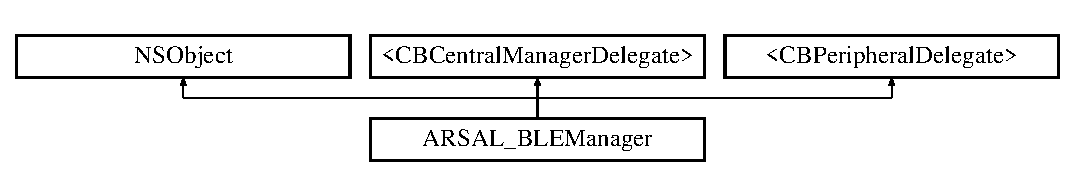
\includegraphics[height=1.934370cm]{interfaceARSAL__BLEManager}
\end{center}
\end{figure}
\subsection*{Instance Methods}
\begin{DoxyCompactItemize}
\item 
(\hyperlink{ARSAL__Error_8h_a95978608019620b9d7e573ad874e5889}{e\+A\+R\+S\+A\+L\+\_\+\+E\+R\+R\+OR}) -\/ \hyperlink{interfaceARSAL__BLEManager_ad4f53997e9972a69ea5d33907f58a08c}{connect\+To\+Peripheral\+:with\+Central\+Manager\+:}
\item 
(void) -\/ \hyperlink{interfaceARSAL__BLEManager_a4bbebe90b27a85c42c2e24496b3ef87a}{disconnect\+Peripheral\+:with\+Central\+Manager\+:}
\item 
(\hyperlink{ARSAL__Error_8h_a95978608019620b9d7e573ad874e5889}{e\+A\+R\+S\+A\+L\+\_\+\+E\+R\+R\+OR}) -\/ \hyperlink{interfaceARSAL__BLEManager_afe64e431550c1a417f8c4bba8725e5cd}{discover\+Network\+Services\+:}
\item 
(\hyperlink{ARSAL__Error_8h_a95978608019620b9d7e573ad874e5889}{e\+A\+R\+S\+A\+L\+\_\+\+E\+R\+R\+OR}) -\/ \hyperlink{interfaceARSAL__BLEManager_ae0cdcbf690a6b37b5aa440338eedea3d}{discover\+Network\+Characteristics\+:for\+Service\+:}
\item 
(\hyperlink{ARSAL__Error_8h_a95978608019620b9d7e573ad874e5889}{e\+A\+R\+S\+A\+L\+\_\+\+E\+R\+R\+OR}) -\/ \hyperlink{interfaceARSAL__BLEManager_aff5bd57546b8e2e337d0d890749be942}{set\+Notification\+Characteristic\+:}
\item 
(B\+O\+OL) -\/ \hyperlink{interfaceARSAL__BLEManager_ae708dcfc73ba14001397bd7a9fabdef5}{write\+Data\+:to\+Characteristic\+:}
\item 
(\hyperlink{ARSAL__Error_8h_a95978608019620b9d7e573ad874e5889}{e\+A\+R\+S\+A\+L\+\_\+\+E\+R\+R\+OR}) -\/ \hyperlink{interfaceARSAL__BLEManager_a9215414f0744c885157a4f705469e482}{write\+Data\+With\+Response\+:to\+Characteristic\+:}
\item 
(B\+O\+OL) -\/ \hyperlink{interfaceARSAL__BLEManager_a456d597ceee1eb99c23ce9f8fe0b7fc1}{is\+Peripheral\+Connected}
\item 
(void) -\/ \hyperlink{interfaceARSAL__BLEManager_a2bfe42d81086019fc3f10c640a8ea14a}{register\+Notification\+Characteristics\+:to\+Key\+:}
\item 
(B\+O\+OL) -\/ \hyperlink{interfaceARSAL__BLEManager_a7ab976168376b677b14075f0d8f1d3cf}{unregister\+Notification\+Characteristics\+:}
\item 
(B\+O\+OL) -\/ \hyperlink{interfaceARSAL__BLEManager_ab9712e7ca6da641483664d1ebdfbc690}{cancel\+Read\+Notification\+:}
\item 
(B\+O\+OL) -\/ \hyperlink{interfaceARSAL__BLEManager_a35c00081083a3cf9716ebfc73adbaeec}{reset\+Read\+Notification\+:}
\item 
(\hyperlink{ARSAL__Error_8h_a95978608019620b9d7e573ad874e5889}{e\+A\+R\+S\+A\+L\+\_\+\+E\+R\+R\+OR}) -\/ \hyperlink{interfaceARSAL__BLEManager_a631ffa16a79854a57ebf744509038859}{read\+Notification\+Data\+:max\+Count\+:timeout\+:to\+Key\+:}
\item 
(void) -\/ \hyperlink{interfaceARSAL__BLEManager_aec8afef362675fb59e03aa2b81c39141}{read\+Data\+:}
\item 
(void) -\/ \hyperlink{interfaceARSAL__BLEManager_af90789b4d2eba4b84a886d689e9a0f56}{unlock}
\item 
(void) -\/ \hyperlink{interfaceARSAL__BLEManager_aa7bfd6655251871a975263ff249b2074}{reset}
\end{DoxyCompactItemize}
\subsection*{Protected Member Functions}
\begin{DoxyCompactItemize}
\item 
() -\/ \hyperlink{interfaceARSAL__BLEManager_aea5e1d03fac306f00ae920a87044020c}{D\+E\+C\+L\+A\+R\+E\+\_\+\+S\+I\+N\+G\+L\+E\+T\+O\+N\+\_\+\+F\+O\+R\+\_\+\+C\+L\+A\+SS}
\end{DoxyCompactItemize}
\subsection*{Protected Attributes}
\begin{DoxyCompactItemize}
\item 
\hyperlink{ARSAL__Sem_8h_a74eaf25f9acaab7ff185cb3c30ffda1c}{A\+R\+S\+A\+L\+\_\+\+Sem\+\_\+t} \hyperlink{interfaceARSAL__BLEManager_a48ce3c205ac6334199a7e0c264a2073d}{connection\+Sem}
\item 
\hyperlink{ARSAL__Sem_8h_a74eaf25f9acaab7ff185cb3c30ffda1c}{A\+R\+S\+A\+L\+\_\+\+Sem\+\_\+t} \hyperlink{interfaceARSAL__BLEManager_a57a0bed8439a2bac7c30f4ee3375daa4}{disconnection\+Sem}
\item 
\hyperlink{ARSAL__Sem_8h_a74eaf25f9acaab7ff185cb3c30ffda1c}{A\+R\+S\+A\+L\+\_\+\+Sem\+\_\+t} \hyperlink{interfaceARSAL__BLEManager_a088ad383094439d68a3c7b617f3e014b}{discover\+Services\+Sem}
\item 
\hyperlink{ARSAL__Sem_8h_a74eaf25f9acaab7ff185cb3c30ffda1c}{A\+R\+S\+A\+L\+\_\+\+Sem\+\_\+t} \hyperlink{interfaceARSAL__BLEManager_a5b4ed96218b90c022292e20047d90628}{discover\+Characteristics\+Sem}
\item 
\hyperlink{ARSAL__Sem_8h_a74eaf25f9acaab7ff185cb3c30ffda1c}{A\+R\+S\+A\+L\+\_\+\+Sem\+\_\+t} \hyperlink{interfaceARSAL__BLEManager_aa6c61e4bd4aba9777de160f538f28850}{write\+Characteristic\+Sem}
\item 
\hyperlink{ARSAL__Sem_8h_a74eaf25f9acaab7ff185cb3c30ffda1c}{A\+R\+S\+A\+L\+\_\+\+Sem\+\_\+t} \hyperlink{interfaceARSAL__BLEManager_ae3c5e30776574be97aa83842636f33f4}{configuration\+Sem}
\end{DoxyCompactItemize}
\subsection*{Properties}
\begin{DoxyCompactItemize}
\item 
id$<$ A\+R\+S\+A\+L\+B\+L\+E\+Manager\+Delegate $>$ \hyperlink{interfaceARSAL__BLEManager_aead3a29e0e0fc9a1dff3bb3f9474dca3}{delegate}
\item 
C\+B\+Peripheral $\ast$ \hyperlink{interfaceARSAL__BLEManager_a2f71424c0b4e400656bdde9be78ad741}{active\+Peripheral}
\item 
N\+S\+Mutable\+Array $\ast$ \hyperlink{interfaceARSAL__BLEManager_ae326962fee96bf58f374fb7d4f3d2260}{characteristics\+Notifications}
\end{DoxyCompactItemize}


\subsection{Method Documentation}
\hypertarget{interfaceARSAL__BLEManager_ab9712e7ca6da641483664d1ebdfbc690}{}\label{interfaceARSAL__BLEManager_ab9712e7ca6da641483664d1ebdfbc690} 
\index{A\+R\+S\+A\+L\+\_\+\+B\+L\+E\+Manager@{A\+R\+S\+A\+L\+\_\+\+B\+L\+E\+Manager}!cancel\+Read\+Notification\+:@{cancel\+Read\+Notification\+:}}
\index{cancel\+Read\+Notification\+:@{cancel\+Read\+Notification\+:}!A\+R\+S\+A\+L\+\_\+\+B\+L\+E\+Manager@{A\+R\+S\+A\+L\+\_\+\+B\+L\+E\+Manager}}
\subsubsection{\texorpdfstring{cancel\+Read\+Notification\+:()}{cancelReadNotification:()}}
{\footnotesize\ttfamily -\/ (B\+O\+OL) cancel\+Read\+Notification\+: \begin{DoxyParamCaption}\item[{(N\+S\+String $\ast$)}]{read\+Characteristics\+Key }\end{DoxyParamCaption}}

\hypertarget{interfaceARSAL__BLEManager_ad4f53997e9972a69ea5d33907f58a08c}{}\label{interfaceARSAL__BLEManager_ad4f53997e9972a69ea5d33907f58a08c} 
\index{A\+R\+S\+A\+L\+\_\+\+B\+L\+E\+Manager@{A\+R\+S\+A\+L\+\_\+\+B\+L\+E\+Manager}!connect\+To\+Peripheral\+:with\+Central\+Manager\+:@{connect\+To\+Peripheral\+:with\+Central\+Manager\+:}}
\index{connect\+To\+Peripheral\+:with\+Central\+Manager\+:@{connect\+To\+Peripheral\+:with\+Central\+Manager\+:}!A\+R\+S\+A\+L\+\_\+\+B\+L\+E\+Manager@{A\+R\+S\+A\+L\+\_\+\+B\+L\+E\+Manager}}
\subsubsection{\texorpdfstring{connect\+To\+Peripheral\+:with\+Central\+Manager\+:()}{connectToPeripheral:withCentralManager:()}}
{\footnotesize\ttfamily -\/ (\hyperlink{ARSAL__Error_8h_a95978608019620b9d7e573ad874e5889}{e\+A\+R\+S\+A\+L\+\_\+\+E\+R\+R\+OR}) connect\+To\+Peripheral\+: \begin{DoxyParamCaption}\item[{(C\+B\+Peripheral $\ast$)}]{peripheral }\item[{withCentralManager:(\hyperlink{interfaceARSAL__CentralManager}{A\+R\+S\+A\+L\+\_\+\+Central\+Manager} $\ast$)}]{central\+Manager }\end{DoxyParamCaption}}

\hypertarget{interfaceARSAL__BLEManager_aea5e1d03fac306f00ae920a87044020c}{}\label{interfaceARSAL__BLEManager_aea5e1d03fac306f00ae920a87044020c} 
\index{A\+R\+S\+A\+L\+\_\+\+B\+L\+E\+Manager@{A\+R\+S\+A\+L\+\_\+\+B\+L\+E\+Manager}!D\+E\+C\+L\+A\+R\+E\+\_\+\+S\+I\+N\+G\+L\+E\+T\+O\+N\+\_\+\+F\+O\+R\+\_\+\+C\+L\+A\+SS@{D\+E\+C\+L\+A\+R\+E\+\_\+\+S\+I\+N\+G\+L\+E\+T\+O\+N\+\_\+\+F\+O\+R\+\_\+\+C\+L\+A\+SS}}
\index{D\+E\+C\+L\+A\+R\+E\+\_\+\+S\+I\+N\+G\+L\+E\+T\+O\+N\+\_\+\+F\+O\+R\+\_\+\+C\+L\+A\+SS@{D\+E\+C\+L\+A\+R\+E\+\_\+\+S\+I\+N\+G\+L\+E\+T\+O\+N\+\_\+\+F\+O\+R\+\_\+\+C\+L\+A\+SS}!A\+R\+S\+A\+L\+\_\+\+B\+L\+E\+Manager@{A\+R\+S\+A\+L\+\_\+\+B\+L\+E\+Manager}}
\subsubsection{\texorpdfstring{D\+E\+C\+L\+A\+R\+E\+\_\+\+S\+I\+N\+G\+L\+E\+T\+O\+N\+\_\+\+F\+O\+R\+\_\+\+C\+L\+A\+S\+S()}{DECLARE\_SINGLETON\_FOR\_CLASS()}}
{\footnotesize\ttfamily -\/ D\+E\+C\+L\+A\+R\+E\+\_\+\+S\+I\+N\+G\+L\+E\+T\+O\+N\+\_\+\+F\+O\+R\+\_\+\+C\+L\+A\+SS \begin{DoxyParamCaption}\item[{(\hyperlink{interfaceARSAL__BLEManager}{A\+R\+S\+A\+L\+\_\+\+B\+L\+E\+Manager})}]{ }\end{DoxyParamCaption}}

\hypertarget{interfaceARSAL__BLEManager_a4bbebe90b27a85c42c2e24496b3ef87a}{}\label{interfaceARSAL__BLEManager_a4bbebe90b27a85c42c2e24496b3ef87a} 
\index{A\+R\+S\+A\+L\+\_\+\+B\+L\+E\+Manager@{A\+R\+S\+A\+L\+\_\+\+B\+L\+E\+Manager}!disconnect\+Peripheral\+:with\+Central\+Manager\+:@{disconnect\+Peripheral\+:with\+Central\+Manager\+:}}
\index{disconnect\+Peripheral\+:with\+Central\+Manager\+:@{disconnect\+Peripheral\+:with\+Central\+Manager\+:}!A\+R\+S\+A\+L\+\_\+\+B\+L\+E\+Manager@{A\+R\+S\+A\+L\+\_\+\+B\+L\+E\+Manager}}
\subsubsection{\texorpdfstring{disconnect\+Peripheral\+:with\+Central\+Manager\+:()}{disconnectPeripheral:withCentralManager:()}}
{\footnotesize\ttfamily -\/ (void) disconnect\+Peripheral\+: \begin{DoxyParamCaption}\item[{(C\+B\+Peripheral $\ast$)}]{peripheral }\item[{withCentralManager:(\hyperlink{interfaceARSAL__CentralManager}{A\+R\+S\+A\+L\+\_\+\+Central\+Manager} $\ast$)}]{central\+Manager }\end{DoxyParamCaption}}

\hypertarget{interfaceARSAL__BLEManager_ae0cdcbf690a6b37b5aa440338eedea3d}{}\label{interfaceARSAL__BLEManager_ae0cdcbf690a6b37b5aa440338eedea3d} 
\index{A\+R\+S\+A\+L\+\_\+\+B\+L\+E\+Manager@{A\+R\+S\+A\+L\+\_\+\+B\+L\+E\+Manager}!discover\+Network\+Characteristics\+:for\+Service\+:@{discover\+Network\+Characteristics\+:for\+Service\+:}}
\index{discover\+Network\+Characteristics\+:for\+Service\+:@{discover\+Network\+Characteristics\+:for\+Service\+:}!A\+R\+S\+A\+L\+\_\+\+B\+L\+E\+Manager@{A\+R\+S\+A\+L\+\_\+\+B\+L\+E\+Manager}}
\subsubsection{\texorpdfstring{discover\+Network\+Characteristics\+:for\+Service\+:()}{discoverNetworkCharacteristics:forService:()}}
{\footnotesize\ttfamily -\/ (\hyperlink{ARSAL__Error_8h_a95978608019620b9d7e573ad874e5889}{e\+A\+R\+S\+A\+L\+\_\+\+E\+R\+R\+OR}) discover\+Network\+Characteristics\+: \begin{DoxyParamCaption}\item[{(N\+S\+Array $\ast$)}]{characteristics\+U\+U\+I\+Ds }\item[{forService:(C\+B\+Service $\ast$)}]{service }\end{DoxyParamCaption}}

\hypertarget{interfaceARSAL__BLEManager_afe64e431550c1a417f8c4bba8725e5cd}{}\label{interfaceARSAL__BLEManager_afe64e431550c1a417f8c4bba8725e5cd} 
\index{A\+R\+S\+A\+L\+\_\+\+B\+L\+E\+Manager@{A\+R\+S\+A\+L\+\_\+\+B\+L\+E\+Manager}!discover\+Network\+Services\+:@{discover\+Network\+Services\+:}}
\index{discover\+Network\+Services\+:@{discover\+Network\+Services\+:}!A\+R\+S\+A\+L\+\_\+\+B\+L\+E\+Manager@{A\+R\+S\+A\+L\+\_\+\+B\+L\+E\+Manager}}
\subsubsection{\texorpdfstring{discover\+Network\+Services\+:()}{discoverNetworkServices:()}}
{\footnotesize\ttfamily -\/ (\hyperlink{ARSAL__Error_8h_a95978608019620b9d7e573ad874e5889}{e\+A\+R\+S\+A\+L\+\_\+\+E\+R\+R\+OR}) discover\+Network\+Services\+: \begin{DoxyParamCaption}\item[{(N\+S\+Array $\ast$)}]{services\+U\+U\+I\+Ds }\end{DoxyParamCaption}}

\hypertarget{interfaceARSAL__BLEManager_a456d597ceee1eb99c23ce9f8fe0b7fc1}{}\label{interfaceARSAL__BLEManager_a456d597ceee1eb99c23ce9f8fe0b7fc1} 
\index{A\+R\+S\+A\+L\+\_\+\+B\+L\+E\+Manager@{A\+R\+S\+A\+L\+\_\+\+B\+L\+E\+Manager}!is\+Peripheral\+Connected@{is\+Peripheral\+Connected}}
\index{is\+Peripheral\+Connected@{is\+Peripheral\+Connected}!A\+R\+S\+A\+L\+\_\+\+B\+L\+E\+Manager@{A\+R\+S\+A\+L\+\_\+\+B\+L\+E\+Manager}}
\subsubsection{\texorpdfstring{is\+Peripheral\+Connected()}{isPeripheralConnected()}}
{\footnotesize\ttfamily -\/ (B\+O\+OL) is\+Peripheral\+Connected \begin{DoxyParamCaption}{ }\end{DoxyParamCaption}}

\hypertarget{interfaceARSAL__BLEManager_aec8afef362675fb59e03aa2b81c39141}{}\label{interfaceARSAL__BLEManager_aec8afef362675fb59e03aa2b81c39141} 
\index{A\+R\+S\+A\+L\+\_\+\+B\+L\+E\+Manager@{A\+R\+S\+A\+L\+\_\+\+B\+L\+E\+Manager}!read\+Data\+:@{read\+Data\+:}}
\index{read\+Data\+:@{read\+Data\+:}!A\+R\+S\+A\+L\+\_\+\+B\+L\+E\+Manager@{A\+R\+S\+A\+L\+\_\+\+B\+L\+E\+Manager}}
\subsubsection{\texorpdfstring{read\+Data\+:()}{readData:()}}
{\footnotesize\ttfamily -\/ (void) read\+Data\+: \begin{DoxyParamCaption}\item[{(C\+B\+Characteristic $\ast$)}]{characteristic }\end{DoxyParamCaption}}

\hypertarget{interfaceARSAL__BLEManager_a631ffa16a79854a57ebf744509038859}{}\label{interfaceARSAL__BLEManager_a631ffa16a79854a57ebf744509038859} 
\index{A\+R\+S\+A\+L\+\_\+\+B\+L\+E\+Manager@{A\+R\+S\+A\+L\+\_\+\+B\+L\+E\+Manager}!read\+Notification\+Data\+:max\+Count\+:timeout\+:to\+Key\+:@{read\+Notification\+Data\+:max\+Count\+:timeout\+:to\+Key\+:}}
\index{read\+Notification\+Data\+:max\+Count\+:timeout\+:to\+Key\+:@{read\+Notification\+Data\+:max\+Count\+:timeout\+:to\+Key\+:}!A\+R\+S\+A\+L\+\_\+\+B\+L\+E\+Manager@{A\+R\+S\+A\+L\+\_\+\+B\+L\+E\+Manager}}
\subsubsection{\texorpdfstring{read\+Notification\+Data\+:max\+Count\+:timeout\+:to\+Key\+:()}{readNotificationData:maxCount:timeout:toKey:()}}
{\footnotesize\ttfamily -\/ (\hyperlink{ARSAL__Error_8h_a95978608019620b9d7e573ad874e5889}{e\+A\+R\+S\+A\+L\+\_\+\+E\+R\+R\+OR}) read\+Notification\+Data\+: \begin{DoxyParamCaption}\item[{(N\+S\+Mutable\+Array $\ast$)}]{notification\+Array }\item[{maxCount:(int)}]{max\+Count }\item[{timeout:(N\+S\+Number $\ast$)}]{timeout }\item[{toKey:(N\+S\+String $\ast$)}]{read\+Characteristics\+Key }\end{DoxyParamCaption}}

\hypertarget{interfaceARSAL__BLEManager_a2bfe42d81086019fc3f10c640a8ea14a}{}\label{interfaceARSAL__BLEManager_a2bfe42d81086019fc3f10c640a8ea14a} 
\index{A\+R\+S\+A\+L\+\_\+\+B\+L\+E\+Manager@{A\+R\+S\+A\+L\+\_\+\+B\+L\+E\+Manager}!register\+Notification\+Characteristics\+:to\+Key\+:@{register\+Notification\+Characteristics\+:to\+Key\+:}}
\index{register\+Notification\+Characteristics\+:to\+Key\+:@{register\+Notification\+Characteristics\+:to\+Key\+:}!A\+R\+S\+A\+L\+\_\+\+B\+L\+E\+Manager@{A\+R\+S\+A\+L\+\_\+\+B\+L\+E\+Manager}}
\subsubsection{\texorpdfstring{register\+Notification\+Characteristics\+:to\+Key\+:()}{registerNotificationCharacteristics:toKey:()}}
{\footnotesize\ttfamily -\/ (void) register\+Notification\+Characteristics\+: \begin{DoxyParamCaption}\item[{(N\+S\+Array $\ast$)}]{characteristics\+Array }\item[{toKey:(N\+S\+String $\ast$)}]{read\+Characteristics\+Key }\end{DoxyParamCaption}}

\hypertarget{interfaceARSAL__BLEManager_aa7bfd6655251871a975263ff249b2074}{}\label{interfaceARSAL__BLEManager_aa7bfd6655251871a975263ff249b2074} 
\index{A\+R\+S\+A\+L\+\_\+\+B\+L\+E\+Manager@{A\+R\+S\+A\+L\+\_\+\+B\+L\+E\+Manager}!reset@{reset}}
\index{reset@{reset}!A\+R\+S\+A\+L\+\_\+\+B\+L\+E\+Manager@{A\+R\+S\+A\+L\+\_\+\+B\+L\+E\+Manager}}
\subsubsection{\texorpdfstring{reset()}{reset()}}
{\footnotesize\ttfamily -\/ (void) reset \begin{DoxyParamCaption}{ }\end{DoxyParamCaption}}

\hypertarget{interfaceARSAL__BLEManager_a35c00081083a3cf9716ebfc73adbaeec}{}\label{interfaceARSAL__BLEManager_a35c00081083a3cf9716ebfc73adbaeec} 
\index{A\+R\+S\+A\+L\+\_\+\+B\+L\+E\+Manager@{A\+R\+S\+A\+L\+\_\+\+B\+L\+E\+Manager}!reset\+Read\+Notification\+:@{reset\+Read\+Notification\+:}}
\index{reset\+Read\+Notification\+:@{reset\+Read\+Notification\+:}!A\+R\+S\+A\+L\+\_\+\+B\+L\+E\+Manager@{A\+R\+S\+A\+L\+\_\+\+B\+L\+E\+Manager}}
\subsubsection{\texorpdfstring{reset\+Read\+Notification\+:()}{resetReadNotification:()}}
{\footnotesize\ttfamily -\/ (B\+O\+OL) reset\+Read\+Notification\+: \begin{DoxyParamCaption}\item[{(N\+S\+String $\ast$)}]{read\+Characteristics\+Key }\end{DoxyParamCaption}}

\hypertarget{interfaceARSAL__BLEManager_aff5bd57546b8e2e337d0d890749be942}{}\label{interfaceARSAL__BLEManager_aff5bd57546b8e2e337d0d890749be942} 
\index{A\+R\+S\+A\+L\+\_\+\+B\+L\+E\+Manager@{A\+R\+S\+A\+L\+\_\+\+B\+L\+E\+Manager}!set\+Notification\+Characteristic\+:@{set\+Notification\+Characteristic\+:}}
\index{set\+Notification\+Characteristic\+:@{set\+Notification\+Characteristic\+:}!A\+R\+S\+A\+L\+\_\+\+B\+L\+E\+Manager@{A\+R\+S\+A\+L\+\_\+\+B\+L\+E\+Manager}}
\subsubsection{\texorpdfstring{set\+Notification\+Characteristic\+:()}{setNotificationCharacteristic:()}}
{\footnotesize\ttfamily -\/ (\hyperlink{ARSAL__Error_8h_a95978608019620b9d7e573ad874e5889}{e\+A\+R\+S\+A\+L\+\_\+\+E\+R\+R\+OR}) set\+Notification\+Characteristic\+: \begin{DoxyParamCaption}\item[{(C\+B\+Characteristic $\ast$)}]{characteristic }\end{DoxyParamCaption}}

\hypertarget{interfaceARSAL__BLEManager_af90789b4d2eba4b84a886d689e9a0f56}{}\label{interfaceARSAL__BLEManager_af90789b4d2eba4b84a886d689e9a0f56} 
\index{A\+R\+S\+A\+L\+\_\+\+B\+L\+E\+Manager@{A\+R\+S\+A\+L\+\_\+\+B\+L\+E\+Manager}!unlock@{unlock}}
\index{unlock@{unlock}!A\+R\+S\+A\+L\+\_\+\+B\+L\+E\+Manager@{A\+R\+S\+A\+L\+\_\+\+B\+L\+E\+Manager}}
\subsubsection{\texorpdfstring{unlock()}{unlock()}}
{\footnotesize\ttfamily -\/ (void) unlock \begin{DoxyParamCaption}{ }\end{DoxyParamCaption}}

\hypertarget{interfaceARSAL__BLEManager_a7ab976168376b677b14075f0d8f1d3cf}{}\label{interfaceARSAL__BLEManager_a7ab976168376b677b14075f0d8f1d3cf} 
\index{A\+R\+S\+A\+L\+\_\+\+B\+L\+E\+Manager@{A\+R\+S\+A\+L\+\_\+\+B\+L\+E\+Manager}!unregister\+Notification\+Characteristics\+:@{unregister\+Notification\+Characteristics\+:}}
\index{unregister\+Notification\+Characteristics\+:@{unregister\+Notification\+Characteristics\+:}!A\+R\+S\+A\+L\+\_\+\+B\+L\+E\+Manager@{A\+R\+S\+A\+L\+\_\+\+B\+L\+E\+Manager}}
\subsubsection{\texorpdfstring{unregister\+Notification\+Characteristics\+:()}{unregisterNotificationCharacteristics:()}}
{\footnotesize\ttfamily -\/ (B\+O\+OL) unregister\+Notification\+Characteristics\+: \begin{DoxyParamCaption}\item[{(N\+S\+String $\ast$)}]{read\+Characteristics\+Key }\end{DoxyParamCaption}}

\hypertarget{interfaceARSAL__BLEManager_ae708dcfc73ba14001397bd7a9fabdef5}{}\label{interfaceARSAL__BLEManager_ae708dcfc73ba14001397bd7a9fabdef5} 
\index{A\+R\+S\+A\+L\+\_\+\+B\+L\+E\+Manager@{A\+R\+S\+A\+L\+\_\+\+B\+L\+E\+Manager}!write\+Data\+:to\+Characteristic\+:@{write\+Data\+:to\+Characteristic\+:}}
\index{write\+Data\+:to\+Characteristic\+:@{write\+Data\+:to\+Characteristic\+:}!A\+R\+S\+A\+L\+\_\+\+B\+L\+E\+Manager@{A\+R\+S\+A\+L\+\_\+\+B\+L\+E\+Manager}}
\subsubsection{\texorpdfstring{write\+Data\+:to\+Characteristic\+:()}{writeData:toCharacteristic:()}}
{\footnotesize\ttfamily -\/ (B\+O\+OL) write\+Data\+: \begin{DoxyParamCaption}\item[{(N\+S\+Data $\ast$)}]{data }\item[{toCharacteristic:(C\+B\+Characteristic $\ast$)}]{characteristic }\end{DoxyParamCaption}}

\hypertarget{interfaceARSAL__BLEManager_a9215414f0744c885157a4f705469e482}{}\label{interfaceARSAL__BLEManager_a9215414f0744c885157a4f705469e482} 
\index{A\+R\+S\+A\+L\+\_\+\+B\+L\+E\+Manager@{A\+R\+S\+A\+L\+\_\+\+B\+L\+E\+Manager}!write\+Data\+With\+Response\+:to\+Characteristic\+:@{write\+Data\+With\+Response\+:to\+Characteristic\+:}}
\index{write\+Data\+With\+Response\+:to\+Characteristic\+:@{write\+Data\+With\+Response\+:to\+Characteristic\+:}!A\+R\+S\+A\+L\+\_\+\+B\+L\+E\+Manager@{A\+R\+S\+A\+L\+\_\+\+B\+L\+E\+Manager}}
\subsubsection{\texorpdfstring{write\+Data\+With\+Response\+:to\+Characteristic\+:()}{writeDataWithResponse:toCharacteristic:()}}
{\footnotesize\ttfamily -\/ (\hyperlink{ARSAL__Error_8h_a95978608019620b9d7e573ad874e5889}{e\+A\+R\+S\+A\+L\+\_\+\+E\+R\+R\+OR}) write\+Data\+With\+Response\+: \begin{DoxyParamCaption}\item[{(N\+S\+Data $\ast$)}]{data }\item[{toCharacteristic:(C\+B\+Characteristic $\ast$)}]{characteristic }\end{DoxyParamCaption}}



\subsection{Member Data Documentation}
\hypertarget{interfaceARSAL__BLEManager_ae3c5e30776574be97aa83842636f33f4}{}\label{interfaceARSAL__BLEManager_ae3c5e30776574be97aa83842636f33f4} 
\index{A\+R\+S\+A\+L\+\_\+\+B\+L\+E\+Manager@{A\+R\+S\+A\+L\+\_\+\+B\+L\+E\+Manager}!configuration\+Sem@{configuration\+Sem}}
\index{configuration\+Sem@{configuration\+Sem}!A\+R\+S\+A\+L\+\_\+\+B\+L\+E\+Manager@{A\+R\+S\+A\+L\+\_\+\+B\+L\+E\+Manager}}
\subsubsection{\texorpdfstring{configuration\+Sem}{configurationSem}}
{\footnotesize\ttfamily -\/ (\hyperlink{ARSAL__Sem_8h_a74eaf25f9acaab7ff185cb3c30ffda1c}{A\+R\+S\+A\+L\+\_\+\+Sem\+\_\+t}) configuration\+Sem\hspace{0.3cm}{\ttfamily [protected]}}

\hypertarget{interfaceARSAL__BLEManager_a48ce3c205ac6334199a7e0c264a2073d}{}\label{interfaceARSAL__BLEManager_a48ce3c205ac6334199a7e0c264a2073d} 
\index{A\+R\+S\+A\+L\+\_\+\+B\+L\+E\+Manager@{A\+R\+S\+A\+L\+\_\+\+B\+L\+E\+Manager}!connection\+Sem@{connection\+Sem}}
\index{connection\+Sem@{connection\+Sem}!A\+R\+S\+A\+L\+\_\+\+B\+L\+E\+Manager@{A\+R\+S\+A\+L\+\_\+\+B\+L\+E\+Manager}}
\subsubsection{\texorpdfstring{connection\+Sem}{connectionSem}}
{\footnotesize\ttfamily -\/ (\hyperlink{ARSAL__Sem_8h_a74eaf25f9acaab7ff185cb3c30ffda1c}{A\+R\+S\+A\+L\+\_\+\+Sem\+\_\+t}) connection\+Sem\hspace{0.3cm}{\ttfamily [protected]}}

\hypertarget{interfaceARSAL__BLEManager_a57a0bed8439a2bac7c30f4ee3375daa4}{}\label{interfaceARSAL__BLEManager_a57a0bed8439a2bac7c30f4ee3375daa4} 
\index{A\+R\+S\+A\+L\+\_\+\+B\+L\+E\+Manager@{A\+R\+S\+A\+L\+\_\+\+B\+L\+E\+Manager}!disconnection\+Sem@{disconnection\+Sem}}
\index{disconnection\+Sem@{disconnection\+Sem}!A\+R\+S\+A\+L\+\_\+\+B\+L\+E\+Manager@{A\+R\+S\+A\+L\+\_\+\+B\+L\+E\+Manager}}
\subsubsection{\texorpdfstring{disconnection\+Sem}{disconnectionSem}}
{\footnotesize\ttfamily -\/ (\hyperlink{ARSAL__Sem_8h_a74eaf25f9acaab7ff185cb3c30ffda1c}{A\+R\+S\+A\+L\+\_\+\+Sem\+\_\+t}) disconnection\+Sem\hspace{0.3cm}{\ttfamily [protected]}}

\hypertarget{interfaceARSAL__BLEManager_a5b4ed96218b90c022292e20047d90628}{}\label{interfaceARSAL__BLEManager_a5b4ed96218b90c022292e20047d90628} 
\index{A\+R\+S\+A\+L\+\_\+\+B\+L\+E\+Manager@{A\+R\+S\+A\+L\+\_\+\+B\+L\+E\+Manager}!discover\+Characteristics\+Sem@{discover\+Characteristics\+Sem}}
\index{discover\+Characteristics\+Sem@{discover\+Characteristics\+Sem}!A\+R\+S\+A\+L\+\_\+\+B\+L\+E\+Manager@{A\+R\+S\+A\+L\+\_\+\+B\+L\+E\+Manager}}
\subsubsection{\texorpdfstring{discover\+Characteristics\+Sem}{discoverCharacteristicsSem}}
{\footnotesize\ttfamily -\/ (\hyperlink{ARSAL__Sem_8h_a74eaf25f9acaab7ff185cb3c30ffda1c}{A\+R\+S\+A\+L\+\_\+\+Sem\+\_\+t}) discover\+Characteristics\+Sem\hspace{0.3cm}{\ttfamily [protected]}}

\hypertarget{interfaceARSAL__BLEManager_a088ad383094439d68a3c7b617f3e014b}{}\label{interfaceARSAL__BLEManager_a088ad383094439d68a3c7b617f3e014b} 
\index{A\+R\+S\+A\+L\+\_\+\+B\+L\+E\+Manager@{A\+R\+S\+A\+L\+\_\+\+B\+L\+E\+Manager}!discover\+Services\+Sem@{discover\+Services\+Sem}}
\index{discover\+Services\+Sem@{discover\+Services\+Sem}!A\+R\+S\+A\+L\+\_\+\+B\+L\+E\+Manager@{A\+R\+S\+A\+L\+\_\+\+B\+L\+E\+Manager}}
\subsubsection{\texorpdfstring{discover\+Services\+Sem}{discoverServicesSem}}
{\footnotesize\ttfamily -\/ (\hyperlink{ARSAL__Sem_8h_a74eaf25f9acaab7ff185cb3c30ffda1c}{A\+R\+S\+A\+L\+\_\+\+Sem\+\_\+t}) discover\+Services\+Sem\hspace{0.3cm}{\ttfamily [protected]}}

\hypertarget{interfaceARSAL__BLEManager_aa6c61e4bd4aba9777de160f538f28850}{}\label{interfaceARSAL__BLEManager_aa6c61e4bd4aba9777de160f538f28850} 
\index{A\+R\+S\+A\+L\+\_\+\+B\+L\+E\+Manager@{A\+R\+S\+A\+L\+\_\+\+B\+L\+E\+Manager}!write\+Characteristic\+Sem@{write\+Characteristic\+Sem}}
\index{write\+Characteristic\+Sem@{write\+Characteristic\+Sem}!A\+R\+S\+A\+L\+\_\+\+B\+L\+E\+Manager@{A\+R\+S\+A\+L\+\_\+\+B\+L\+E\+Manager}}
\subsubsection{\texorpdfstring{write\+Characteristic\+Sem}{writeCharacteristicSem}}
{\footnotesize\ttfamily -\/ (\hyperlink{ARSAL__Sem_8h_a74eaf25f9acaab7ff185cb3c30ffda1c}{A\+R\+S\+A\+L\+\_\+\+Sem\+\_\+t}) write\+Characteristic\+Sem\hspace{0.3cm}{\ttfamily [protected]}}



\subsection{Property Documentation}
\hypertarget{interfaceARSAL__BLEManager_a2f71424c0b4e400656bdde9be78ad741}{}\label{interfaceARSAL__BLEManager_a2f71424c0b4e400656bdde9be78ad741} 
\index{A\+R\+S\+A\+L\+\_\+\+B\+L\+E\+Manager@{A\+R\+S\+A\+L\+\_\+\+B\+L\+E\+Manager}!active\+Peripheral@{active\+Peripheral}}
\index{active\+Peripheral@{active\+Peripheral}!A\+R\+S\+A\+L\+\_\+\+B\+L\+E\+Manager@{A\+R\+S\+A\+L\+\_\+\+B\+L\+E\+Manager}}
\subsubsection{\texorpdfstring{active\+Peripheral}{activePeripheral}}
{\footnotesize\ttfamily -\/ (C\+B\+Peripheral$\ast$) active\+Peripheral\hspace{0.3cm}{\ttfamily [read]}, {\ttfamily [write]}, {\ttfamily [nonatomic]}, {\ttfamily [retain]}}

\hypertarget{interfaceARSAL__BLEManager_ae326962fee96bf58f374fb7d4f3d2260}{}\label{interfaceARSAL__BLEManager_ae326962fee96bf58f374fb7d4f3d2260} 
\index{A\+R\+S\+A\+L\+\_\+\+B\+L\+E\+Manager@{A\+R\+S\+A\+L\+\_\+\+B\+L\+E\+Manager}!characteristics\+Notifications@{characteristics\+Notifications}}
\index{characteristics\+Notifications@{characteristics\+Notifications}!A\+R\+S\+A\+L\+\_\+\+B\+L\+E\+Manager@{A\+R\+S\+A\+L\+\_\+\+B\+L\+E\+Manager}}
\subsubsection{\texorpdfstring{characteristics\+Notifications}{characteristicsNotifications}}
{\footnotesize\ttfamily -\/ (N\+S\+Mutable\+Array$\ast$) characteristics\+Notifications\hspace{0.3cm}{\ttfamily [read]}, {\ttfamily [write]}, {\ttfamily [nonatomic]}, {\ttfamily [retain]}}

\hypertarget{interfaceARSAL__BLEManager_aead3a29e0e0fc9a1dff3bb3f9474dca3}{}\label{interfaceARSAL__BLEManager_aead3a29e0e0fc9a1dff3bb3f9474dca3} 
\index{A\+R\+S\+A\+L\+\_\+\+B\+L\+E\+Manager@{A\+R\+S\+A\+L\+\_\+\+B\+L\+E\+Manager}!delegate@{delegate}}
\index{delegate@{delegate}!A\+R\+S\+A\+L\+\_\+\+B\+L\+E\+Manager@{A\+R\+S\+A\+L\+\_\+\+B\+L\+E\+Manager}}
\subsubsection{\texorpdfstring{delegate}{delegate}}
{\footnotesize\ttfamily -\/ (id$<$A\+R\+S\+A\+L\+B\+L\+E\+Manager\+Delegate$>$) delegate\hspace{0.3cm}{\ttfamily [read]}, {\ttfamily [write]}, {\ttfamily [nonatomic]}, {\ttfamily [assign]}}



The documentation for this class was generated from the following file\+:\begin{DoxyCompactItemize}
\item 
\hyperlink{ARSAL__BLEManager_8h}{A\+R\+S\+A\+L\+\_\+\+B\+L\+E\+Manager.\+h}\end{DoxyCompactItemize}

\hypertarget{interfaceARSAL__CentralManager}{}\section{A\+R\+S\+A\+L\+\_\+\+Central\+Manager Class Reference}
\label{interfaceARSAL__CentralManager}\index{A\+R\+S\+A\+L\+\_\+\+Central\+Manager@{A\+R\+S\+A\+L\+\_\+\+Central\+Manager}}


{\ttfamily \#import $<$A\+R\+S\+A\+L\+\_\+\+Central\+Manager.\+h$>$}

Inheritance diagram for A\+R\+S\+A\+L\+\_\+\+Central\+Manager\+:\begin{figure}[H]
\begin{center}
\leavevmode
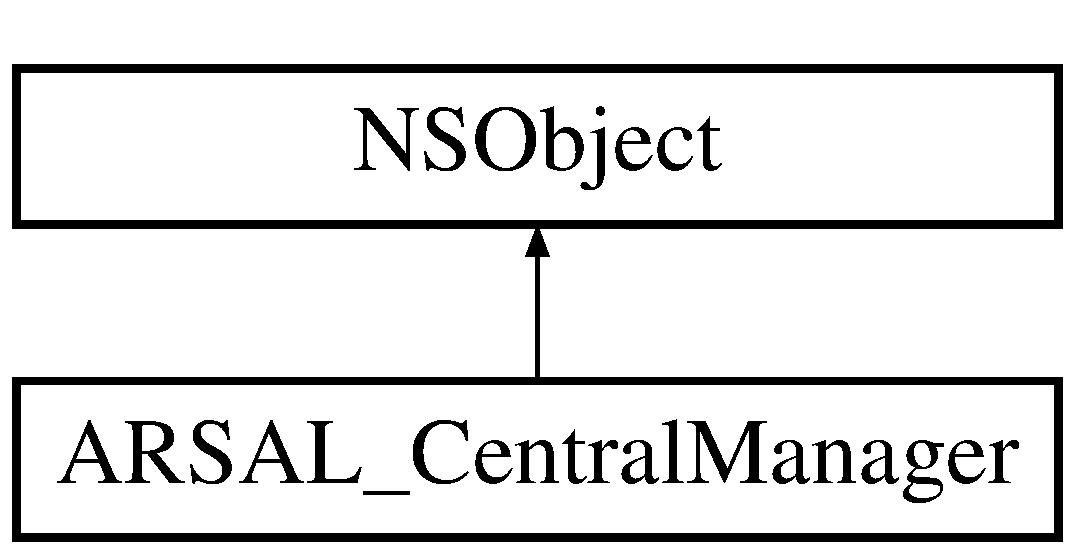
\includegraphics[height=2.000000cm]{interfaceARSAL__CentralManager}
\end{center}
\end{figure}
\subsection*{Instance Methods}
\begin{DoxyCompactItemize}
\item 
(void) -\/ \hyperlink{interfaceARSAL__CentralManager_a33777e4ba7350c283985eb1543f66618}{init\+A\+R\+C\+B\+Central\+Manager\+:options\+:}
\item 
(id) -\/ \hyperlink{interfaceARSAL__CentralManager_a5f8453573494c372cf620f45a77aa3d4}{init\+With\+Queue\+:}
\item 
(id) -\/ \hyperlink{interfaceARSAL__CentralManager_a210798b430593e8dda10b720d05d0804}{init\+With\+Delegate\+:queue\+:options\+:}
\item 
(void) -\/ \hyperlink{interfaceARSAL__CentralManager_aa5f722e581a7b704675dacdca5f9bd5e}{add\+Delegate\+:}
\item 
(void) -\/ \hyperlink{interfaceARSAL__CentralManager_a8cf717c255f5228ced0c72c3b0c20ff9}{remove\+Delegate\+:}
\item 
(void) -\/ \hyperlink{interfaceARSAL__CentralManager_a4902ef59666d20f7964179a184435be8}{connect\+Peripheral\+:options\+:}
\item 
(void) -\/ \hyperlink{interfaceARSAL__CentralManager_a9e0a82a9de4683aab71c38aade16a2c2}{cancel\+Peripheral\+Connection\+:}
\item 
(void) -\/ \hyperlink{interfaceARSAL__CentralManager_a2db3036b3d65aee5d4d5c971685142ef}{scan\+For\+Peripherals\+With\+Services\+:options\+:}
\item 
(void) -\/ \hyperlink{interfaceARSAL__CentralManager_af249376b57f0da90f621e2218c649aa5}{stop\+Scan}
\item 
(N\+S\+Array $\ast$) -\/ \hyperlink{interfaceARSAL__CentralManager_ae7e88c2aefe924068d9930e560716559}{retrieve\+Connected\+Peripherals\+With\+Services\+:}
\item 
(N\+S\+Array $\ast$) -\/ \hyperlink{interfaceARSAL__CentralManager_a75908f30d71bc7cae87dbfdac97d1396}{retrieve\+Peripherals\+With\+Identifiers\+:}
\end{DoxyCompactItemize}


\subsection{Method Documentation}
\hypertarget{interfaceARSAL__CentralManager_aa5f722e581a7b704675dacdca5f9bd5e}{}\label{interfaceARSAL__CentralManager_aa5f722e581a7b704675dacdca5f9bd5e} 
\index{A\+R\+S\+A\+L\+\_\+\+Central\+Manager@{A\+R\+S\+A\+L\+\_\+\+Central\+Manager}!add\+Delegate\+:@{add\+Delegate\+:}}
\index{add\+Delegate\+:@{add\+Delegate\+:}!A\+R\+S\+A\+L\+\_\+\+Central\+Manager@{A\+R\+S\+A\+L\+\_\+\+Central\+Manager}}
\subsubsection{\texorpdfstring{add\+Delegate\+:()}{addDelegate:()}}
{\footnotesize\ttfamily -\/ (void) add\+Delegate\+: \begin{DoxyParamCaption}\item[{(id$<$ C\+B\+Central\+Manager\+Delegate $>$)}]{delegate }\end{DoxyParamCaption}}

\hypertarget{interfaceARSAL__CentralManager_a9e0a82a9de4683aab71c38aade16a2c2}{}\label{interfaceARSAL__CentralManager_a9e0a82a9de4683aab71c38aade16a2c2} 
\index{A\+R\+S\+A\+L\+\_\+\+Central\+Manager@{A\+R\+S\+A\+L\+\_\+\+Central\+Manager}!cancel\+Peripheral\+Connection\+:@{cancel\+Peripheral\+Connection\+:}}
\index{cancel\+Peripheral\+Connection\+:@{cancel\+Peripheral\+Connection\+:}!A\+R\+S\+A\+L\+\_\+\+Central\+Manager@{A\+R\+S\+A\+L\+\_\+\+Central\+Manager}}
\subsubsection{\texorpdfstring{cancel\+Peripheral\+Connection\+:()}{cancelPeripheralConnection:()}}
{\footnotesize\ttfamily -\/ (void) cancel\+Peripheral\+Connection\+: \begin{DoxyParamCaption}\item[{(C\+B\+Peripheral $\ast$)}]{peripheral }\end{DoxyParamCaption}}

\hypertarget{interfaceARSAL__CentralManager_a4902ef59666d20f7964179a184435be8}{}\label{interfaceARSAL__CentralManager_a4902ef59666d20f7964179a184435be8} 
\index{A\+R\+S\+A\+L\+\_\+\+Central\+Manager@{A\+R\+S\+A\+L\+\_\+\+Central\+Manager}!connect\+Peripheral\+:options\+:@{connect\+Peripheral\+:options\+:}}
\index{connect\+Peripheral\+:options\+:@{connect\+Peripheral\+:options\+:}!A\+R\+S\+A\+L\+\_\+\+Central\+Manager@{A\+R\+S\+A\+L\+\_\+\+Central\+Manager}}
\subsubsection{\texorpdfstring{connect\+Peripheral\+:options\+:()}{connectPeripheral:options:()}}
{\footnotesize\ttfamily -\/ (void) connect\+Peripheral\+: \begin{DoxyParamCaption}\item[{(C\+B\+Peripheral $\ast$)}]{peripheral }\item[{options:(N\+S\+Dictionary $\ast$)}]{options }\end{DoxyParamCaption}}

\hypertarget{interfaceARSAL__CentralManager_a33777e4ba7350c283985eb1543f66618}{}\label{interfaceARSAL__CentralManager_a33777e4ba7350c283985eb1543f66618} 
\index{A\+R\+S\+A\+L\+\_\+\+Central\+Manager@{A\+R\+S\+A\+L\+\_\+\+Central\+Manager}!init\+A\+R\+C\+B\+Central\+Manager\+:options\+:@{init\+A\+R\+C\+B\+Central\+Manager\+:options\+:}}
\index{init\+A\+R\+C\+B\+Central\+Manager\+:options\+:@{init\+A\+R\+C\+B\+Central\+Manager\+:options\+:}!A\+R\+S\+A\+L\+\_\+\+Central\+Manager@{A\+R\+S\+A\+L\+\_\+\+Central\+Manager}}
\subsubsection{\texorpdfstring{init\+A\+R\+C\+B\+Central\+Manager\+:options\+:()}{initARCBCentralManager:options:()}}
{\footnotesize\ttfamily -\/ (void) init\+A\+R\+C\+B\+Central\+Manager\+: \begin{DoxyParamCaption}\item[{(dispatch\+\_\+queue\+\_\+t)}]{queue }\item[{options:(N\+S\+Dictionary $\ast$)}]{options }\end{DoxyParamCaption}}

\hypertarget{interfaceARSAL__CentralManager_a210798b430593e8dda10b720d05d0804}{}\label{interfaceARSAL__CentralManager_a210798b430593e8dda10b720d05d0804} 
\index{A\+R\+S\+A\+L\+\_\+\+Central\+Manager@{A\+R\+S\+A\+L\+\_\+\+Central\+Manager}!init\+With\+Delegate\+:queue\+:options\+:@{init\+With\+Delegate\+:queue\+:options\+:}}
\index{init\+With\+Delegate\+:queue\+:options\+:@{init\+With\+Delegate\+:queue\+:options\+:}!A\+R\+S\+A\+L\+\_\+\+Central\+Manager@{A\+R\+S\+A\+L\+\_\+\+Central\+Manager}}
\subsubsection{\texorpdfstring{init\+With\+Delegate\+:queue\+:options\+:()}{initWithDelegate:queue:options:()}}
{\footnotesize\ttfamily -\/ (id) init\+With\+Delegate\+: \begin{DoxyParamCaption}\item[{(id$<$ C\+B\+Central\+Manager\+Delegate $>$)}]{delegate }\item[{queue:(dispatch\+\_\+queue\+\_\+t)}]{queue }\item[{options:(N\+S\+Dictionary $\ast$)}]{options }\end{DoxyParamCaption}}

\hypertarget{interfaceARSAL__CentralManager_a5f8453573494c372cf620f45a77aa3d4}{}\label{interfaceARSAL__CentralManager_a5f8453573494c372cf620f45a77aa3d4} 
\index{A\+R\+S\+A\+L\+\_\+\+Central\+Manager@{A\+R\+S\+A\+L\+\_\+\+Central\+Manager}!init\+With\+Queue\+:@{init\+With\+Queue\+:}}
\index{init\+With\+Queue\+:@{init\+With\+Queue\+:}!A\+R\+S\+A\+L\+\_\+\+Central\+Manager@{A\+R\+S\+A\+L\+\_\+\+Central\+Manager}}
\subsubsection{\texorpdfstring{init\+With\+Queue\+:()}{initWithQueue:()}}
{\footnotesize\ttfamily -\/ (id) init\+With\+Queue\+: \begin{DoxyParamCaption}\item[{(dispatch\+\_\+queue\+\_\+t)}]{queue }\end{DoxyParamCaption}}

\hypertarget{interfaceARSAL__CentralManager_a8cf717c255f5228ced0c72c3b0c20ff9}{}\label{interfaceARSAL__CentralManager_a8cf717c255f5228ced0c72c3b0c20ff9} 
\index{A\+R\+S\+A\+L\+\_\+\+Central\+Manager@{A\+R\+S\+A\+L\+\_\+\+Central\+Manager}!remove\+Delegate\+:@{remove\+Delegate\+:}}
\index{remove\+Delegate\+:@{remove\+Delegate\+:}!A\+R\+S\+A\+L\+\_\+\+Central\+Manager@{A\+R\+S\+A\+L\+\_\+\+Central\+Manager}}
\subsubsection{\texorpdfstring{remove\+Delegate\+:()}{removeDelegate:()}}
{\footnotesize\ttfamily -\/ (void) remove\+Delegate\+: \begin{DoxyParamCaption}\item[{(id$<$ C\+B\+Central\+Manager\+Delegate $>$)}]{delegate }\end{DoxyParamCaption}}

\hypertarget{interfaceARSAL__CentralManager_ae7e88c2aefe924068d9930e560716559}{}\label{interfaceARSAL__CentralManager_ae7e88c2aefe924068d9930e560716559} 
\index{A\+R\+S\+A\+L\+\_\+\+Central\+Manager@{A\+R\+S\+A\+L\+\_\+\+Central\+Manager}!retrieve\+Connected\+Peripherals\+With\+Services\+:@{retrieve\+Connected\+Peripherals\+With\+Services\+:}}
\index{retrieve\+Connected\+Peripherals\+With\+Services\+:@{retrieve\+Connected\+Peripherals\+With\+Services\+:}!A\+R\+S\+A\+L\+\_\+\+Central\+Manager@{A\+R\+S\+A\+L\+\_\+\+Central\+Manager}}
\subsubsection{\texorpdfstring{retrieve\+Connected\+Peripherals\+With\+Services\+:()}{retrieveConnectedPeripheralsWithServices:()}}
{\footnotesize\ttfamily -\/ (N\+S\+Array $\ast$) retrieve\+Connected\+Peripherals\+With\+Services\+: \begin{DoxyParamCaption}\item[{(N\+S\+Array $\ast$)}]{service\+U\+U\+I\+Ds }\end{DoxyParamCaption}}

\hypertarget{interfaceARSAL__CentralManager_a75908f30d71bc7cae87dbfdac97d1396}{}\label{interfaceARSAL__CentralManager_a75908f30d71bc7cae87dbfdac97d1396} 
\index{A\+R\+S\+A\+L\+\_\+\+Central\+Manager@{A\+R\+S\+A\+L\+\_\+\+Central\+Manager}!retrieve\+Peripherals\+With\+Identifiers\+:@{retrieve\+Peripherals\+With\+Identifiers\+:}}
\index{retrieve\+Peripherals\+With\+Identifiers\+:@{retrieve\+Peripherals\+With\+Identifiers\+:}!A\+R\+S\+A\+L\+\_\+\+Central\+Manager@{A\+R\+S\+A\+L\+\_\+\+Central\+Manager}}
\subsubsection{\texorpdfstring{retrieve\+Peripherals\+With\+Identifiers\+:()}{retrievePeripheralsWithIdentifiers:()}}
{\footnotesize\ttfamily -\/ (N\+S\+Array $\ast$) retrieve\+Peripherals\+With\+Identifiers\+: \begin{DoxyParamCaption}\item[{(N\+S\+Array $\ast$)}]{identifiers }\end{DoxyParamCaption}}

\hypertarget{interfaceARSAL__CentralManager_a2db3036b3d65aee5d4d5c971685142ef}{}\label{interfaceARSAL__CentralManager_a2db3036b3d65aee5d4d5c971685142ef} 
\index{A\+R\+S\+A\+L\+\_\+\+Central\+Manager@{A\+R\+S\+A\+L\+\_\+\+Central\+Manager}!scan\+For\+Peripherals\+With\+Services\+:options\+:@{scan\+For\+Peripherals\+With\+Services\+:options\+:}}
\index{scan\+For\+Peripherals\+With\+Services\+:options\+:@{scan\+For\+Peripherals\+With\+Services\+:options\+:}!A\+R\+S\+A\+L\+\_\+\+Central\+Manager@{A\+R\+S\+A\+L\+\_\+\+Central\+Manager}}
\subsubsection{\texorpdfstring{scan\+For\+Peripherals\+With\+Services\+:options\+:()}{scanForPeripheralsWithServices:options:()}}
{\footnotesize\ttfamily -\/ (void) scan\+For\+Peripherals\+With\+Services\+: \begin{DoxyParamCaption}\item[{(N\+S\+Array $\ast$)}]{service\+U\+U\+I\+Ds }\item[{options:(N\+S\+Dictionary $\ast$)}]{options }\end{DoxyParamCaption}}

\hypertarget{interfaceARSAL__CentralManager_af249376b57f0da90f621e2218c649aa5}{}\label{interfaceARSAL__CentralManager_af249376b57f0da90f621e2218c649aa5} 
\index{A\+R\+S\+A\+L\+\_\+\+Central\+Manager@{A\+R\+S\+A\+L\+\_\+\+Central\+Manager}!stop\+Scan@{stop\+Scan}}
\index{stop\+Scan@{stop\+Scan}!A\+R\+S\+A\+L\+\_\+\+Central\+Manager@{A\+R\+S\+A\+L\+\_\+\+Central\+Manager}}
\subsubsection{\texorpdfstring{stop\+Scan()}{stopScan()}}
{\footnotesize\ttfamily -\/ (void) stop\+Scan \begin{DoxyParamCaption}{ }\end{DoxyParamCaption}}



The documentation for this class was generated from the following file\+:\begin{DoxyCompactItemize}
\item 
\hyperlink{ARSAL__CentralManager_8h}{A\+R\+S\+A\+L\+\_\+\+Central\+Manager.\+h}\end{DoxyCompactItemize}

\hypertarget{protocolARSALBLEManagerDelegate_01-p}{}\section{$<$A\+R\+S\+A\+L\+B\+L\+E\+Manager\+Delegate $>$ Protocol Reference}
\label{protocolARSALBLEManagerDelegate_01-p}\index{$<$\+A\+R\+S\+A\+L\+B\+L\+E\+Manager\+Delegate $>$@{$<$\+A\+R\+S\+A\+L\+B\+L\+E\+Manager\+Delegate $>$}}


{\ttfamily \#import $<$A\+R\+S\+A\+L\+\_\+\+B\+L\+E\+Manager.\+h$>$}

Inheritance diagram for $<$A\+R\+S\+A\+L\+B\+L\+E\+Manager\+Delegate $>$\+:\begin{figure}[H]
\begin{center}
\leavevmode
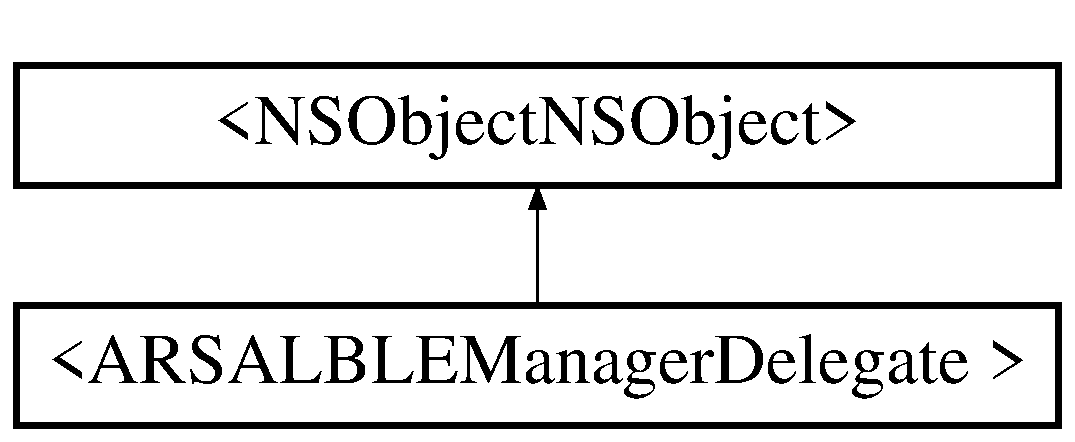
\includegraphics[height=2.000000cm]{protocolARSALBLEManagerDelegate_01-p}
\end{center}
\end{figure}
\subsection*{Instance Methods}
\begin{DoxyCompactItemize}
\item 
(void) -\/ \hyperlink{protocolARSALBLEManagerDelegate_01-p_aaf4b420056f1e8f8808c110f426e61d1}{on\+B\+L\+E\+Disconnect}
\end{DoxyCompactItemize}


\subsection{Method Documentation}
\hypertarget{protocolARSALBLEManagerDelegate_01-p_aaf4b420056f1e8f8808c110f426e61d1}{}\label{protocolARSALBLEManagerDelegate_01-p_aaf4b420056f1e8f8808c110f426e61d1} 
\index{A\+R\+S\+A\+L\+B\+L\+E\+Manager\+Delegate -\/p@{A\+R\+S\+A\+L\+B\+L\+E\+Manager\+Delegate -\/p}!on\+B\+L\+E\+Disconnect@{on\+B\+L\+E\+Disconnect}}
\index{on\+B\+L\+E\+Disconnect@{on\+B\+L\+E\+Disconnect}!A\+R\+S\+A\+L\+B\+L\+E\+Manager\+Delegate -\/p@{A\+R\+S\+A\+L\+B\+L\+E\+Manager\+Delegate -\/p}}
\subsubsection{\texorpdfstring{on\+B\+L\+E\+Disconnect()}{onBLEDisconnect()}}
{\footnotesize\ttfamily -\/ (void A\+R\+S\+A\+L\+B\+L\+E\+Manager\+Delegate) on\+B\+L\+E\+Disconnect \begin{DoxyParamCaption}{ }\end{DoxyParamCaption}\hspace{0.3cm}{\ttfamily [required]}}



The documentation for this protocol was generated from the following file\+:\begin{DoxyCompactItemize}
\item 
\hyperlink{ARSAL__BLEManager_8h}{A\+R\+S\+A\+L\+\_\+\+B\+L\+E\+Manager.\+h}\end{DoxyCompactItemize}

\hypertarget{interfaceARSALBLEManagerNotification}{}\section{A\+R\+S\+A\+L\+B\+L\+E\+Manager\+Notification Class Reference}
\label{interfaceARSALBLEManagerNotification}\index{A\+R\+S\+A\+L\+B\+L\+E\+Manager\+Notification@{A\+R\+S\+A\+L\+B\+L\+E\+Manager\+Notification}}


{\ttfamily \#import $<$A\+R\+S\+A\+L\+\_\+\+B\+L\+E\+Manager.\+h$>$}

Inheritance diagram for A\+R\+S\+A\+L\+B\+L\+E\+Manager\+Notification\+:\begin{figure}[H]
\begin{center}
\leavevmode
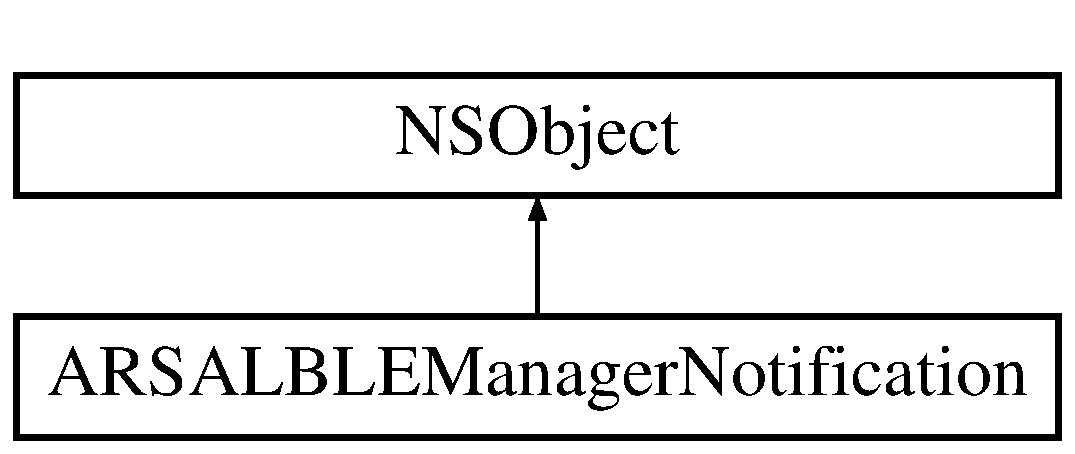
\includegraphics[height=2.000000cm]{interfaceARSALBLEManagerNotification}
\end{center}
\end{figure}
\subsection*{Protected Attributes}
\begin{DoxyCompactItemize}
\item 
\hyperlink{ARSAL__Sem_8h_a74eaf25f9acaab7ff185cb3c30ffda1c}{A\+R\+S\+A\+L\+\_\+\+Sem\+\_\+t} \hyperlink{interfaceARSALBLEManagerNotification_a3aee56e9a10b2d50f2302ab6470bd355}{read\+Characteristics\+Sem}
\item 
\hyperlink{ARSAL__Mutex_8h_a6ad002456ab5e96d6bd51a0df06f0f57}{A\+R\+S\+A\+L\+\_\+\+Mutex\+\_\+t} \hyperlink{interfaceARSALBLEManagerNotification_a687c5dd539262acf0b31ab485dcb885d}{read\+Characteristic\+Mutex}
\end{DoxyCompactItemize}
\subsection*{Properties}
\begin{DoxyCompactItemize}
\item 
N\+S\+Array $\ast$ \hyperlink{interfaceARSALBLEManagerNotification_a8f917b047e82a91e94467bfe22f35ff4}{characteristics}
\item 
N\+S\+Mutable\+Array $\ast$ \hyperlink{interfaceARSALBLEManagerNotification_a8584e955f261031e6e713dbe7d1a1879}{notifications\+Array}
\end{DoxyCompactItemize}


\subsection{Member Data Documentation}
\hypertarget{interfaceARSALBLEManagerNotification_a687c5dd539262acf0b31ab485dcb885d}{}\label{interfaceARSALBLEManagerNotification_a687c5dd539262acf0b31ab485dcb885d} 
\index{A\+R\+S\+A\+L\+B\+L\+E\+Manager\+Notification@{A\+R\+S\+A\+L\+B\+L\+E\+Manager\+Notification}!read\+Characteristic\+Mutex@{read\+Characteristic\+Mutex}}
\index{read\+Characteristic\+Mutex@{read\+Characteristic\+Mutex}!A\+R\+S\+A\+L\+B\+L\+E\+Manager\+Notification@{A\+R\+S\+A\+L\+B\+L\+E\+Manager\+Notification}}
\subsubsection{\texorpdfstring{read\+Characteristic\+Mutex}{readCharacteristicMutex}}
{\footnotesize\ttfamily -\/ (\hyperlink{ARSAL__Mutex_8h_a6ad002456ab5e96d6bd51a0df06f0f57}{A\+R\+S\+A\+L\+\_\+\+Mutex\+\_\+t}) read\+Characteristic\+Mutex\hspace{0.3cm}{\ttfamily [protected]}}

\hypertarget{interfaceARSALBLEManagerNotification_a3aee56e9a10b2d50f2302ab6470bd355}{}\label{interfaceARSALBLEManagerNotification_a3aee56e9a10b2d50f2302ab6470bd355} 
\index{A\+R\+S\+A\+L\+B\+L\+E\+Manager\+Notification@{A\+R\+S\+A\+L\+B\+L\+E\+Manager\+Notification}!read\+Characteristics\+Sem@{read\+Characteristics\+Sem}}
\index{read\+Characteristics\+Sem@{read\+Characteristics\+Sem}!A\+R\+S\+A\+L\+B\+L\+E\+Manager\+Notification@{A\+R\+S\+A\+L\+B\+L\+E\+Manager\+Notification}}
\subsubsection{\texorpdfstring{read\+Characteristics\+Sem}{readCharacteristicsSem}}
{\footnotesize\ttfamily -\/ (\hyperlink{ARSAL__Sem_8h_a74eaf25f9acaab7ff185cb3c30ffda1c}{A\+R\+S\+A\+L\+\_\+\+Sem\+\_\+t}) read\+Characteristics\+Sem\hspace{0.3cm}{\ttfamily [protected]}}



\subsection{Property Documentation}
\hypertarget{interfaceARSALBLEManagerNotification_a8f917b047e82a91e94467bfe22f35ff4}{}\label{interfaceARSALBLEManagerNotification_a8f917b047e82a91e94467bfe22f35ff4} 
\index{A\+R\+S\+A\+L\+B\+L\+E\+Manager\+Notification@{A\+R\+S\+A\+L\+B\+L\+E\+Manager\+Notification}!characteristics@{characteristics}}
\index{characteristics@{characteristics}!A\+R\+S\+A\+L\+B\+L\+E\+Manager\+Notification@{A\+R\+S\+A\+L\+B\+L\+E\+Manager\+Notification}}
\subsubsection{\texorpdfstring{characteristics}{characteristics}}
{\footnotesize\ttfamily -\/ (N\+S\+Array$\ast$) characteristics\hspace{0.3cm}{\ttfamily [read]}, {\ttfamily [write]}, {\ttfamily [nonatomic]}, {\ttfamily [retain]}}

\hypertarget{interfaceARSALBLEManagerNotification_a8584e955f261031e6e713dbe7d1a1879}{}\label{interfaceARSALBLEManagerNotification_a8584e955f261031e6e713dbe7d1a1879} 
\index{A\+R\+S\+A\+L\+B\+L\+E\+Manager\+Notification@{A\+R\+S\+A\+L\+B\+L\+E\+Manager\+Notification}!notifications\+Array@{notifications\+Array}}
\index{notifications\+Array@{notifications\+Array}!A\+R\+S\+A\+L\+B\+L\+E\+Manager\+Notification@{A\+R\+S\+A\+L\+B\+L\+E\+Manager\+Notification}}
\subsubsection{\texorpdfstring{notifications\+Array}{notificationsArray}}
{\footnotesize\ttfamily -\/ (N\+S\+Mutable\+Array$\ast$) notifications\+Array\hspace{0.3cm}{\ttfamily [read]}, {\ttfamily [write]}, {\ttfamily [nonatomic]}, {\ttfamily [retain]}}



The documentation for this class was generated from the following file\+:\begin{DoxyCompactItemize}
\item 
\hyperlink{ARSAL__BLEManager_8h}{A\+R\+S\+A\+L\+\_\+\+B\+L\+E\+Manager.\+h}\end{DoxyCompactItemize}

\hypertarget{interfaceARSALBLEManagerNotificationData}{}\section{A\+R\+S\+A\+L\+B\+L\+E\+Manager\+Notification\+Data Class Reference}
\label{interfaceARSALBLEManagerNotificationData}\index{A\+R\+S\+A\+L\+B\+L\+E\+Manager\+Notification\+Data@{A\+R\+S\+A\+L\+B\+L\+E\+Manager\+Notification\+Data}}


{\ttfamily \#import $<$A\+R\+S\+A\+L\+\_\+\+B\+L\+E\+Manager.\+h$>$}

Inheritance diagram for A\+R\+S\+A\+L\+B\+L\+E\+Manager\+Notification\+Data\+:\begin{figure}[H]
\begin{center}
\leavevmode
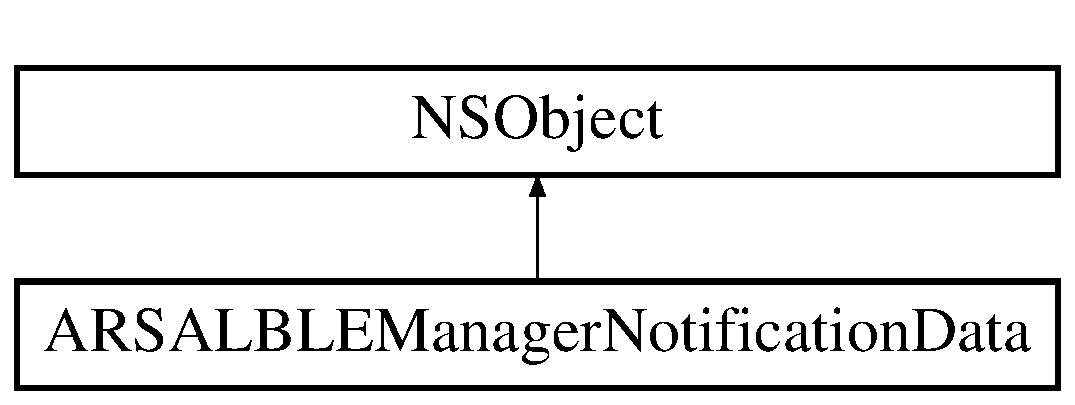
\includegraphics[height=2.000000cm]{interfaceARSALBLEManagerNotificationData}
\end{center}
\end{figure}
\subsection*{Properties}
\begin{DoxyCompactItemize}
\item 
C\+B\+Characteristic $\ast$ \hyperlink{interfaceARSALBLEManagerNotificationData_a2a13532ac913be87b8e8c708859d96ea}{characteristic}
\item 
N\+S\+Data $\ast$ \hyperlink{interfaceARSALBLEManagerNotificationData_ad946383fc336fd155e1a1a087ee230f4}{value}
\end{DoxyCompactItemize}


\subsection{Property Documentation}
\hypertarget{interfaceARSALBLEManagerNotificationData_a2a13532ac913be87b8e8c708859d96ea}{}\label{interfaceARSALBLEManagerNotificationData_a2a13532ac913be87b8e8c708859d96ea} 
\index{A\+R\+S\+A\+L\+B\+L\+E\+Manager\+Notification\+Data@{A\+R\+S\+A\+L\+B\+L\+E\+Manager\+Notification\+Data}!characteristic@{characteristic}}
\index{characteristic@{characteristic}!A\+R\+S\+A\+L\+B\+L\+E\+Manager\+Notification\+Data@{A\+R\+S\+A\+L\+B\+L\+E\+Manager\+Notification\+Data}}
\subsubsection{\texorpdfstring{characteristic}{characteristic}}
{\footnotesize\ttfamily -\/ (C\+B\+Characteristic$\ast$) characteristic\hspace{0.3cm}{\ttfamily [read]}, {\ttfamily [write]}, {\ttfamily [nonatomic]}, {\ttfamily [retain]}}

\hypertarget{interfaceARSALBLEManagerNotificationData_ad946383fc336fd155e1a1a087ee230f4}{}\label{interfaceARSALBLEManagerNotificationData_ad946383fc336fd155e1a1a087ee230f4} 
\index{A\+R\+S\+A\+L\+B\+L\+E\+Manager\+Notification\+Data@{A\+R\+S\+A\+L\+B\+L\+E\+Manager\+Notification\+Data}!value@{value}}
\index{value@{value}!A\+R\+S\+A\+L\+B\+L\+E\+Manager\+Notification\+Data@{A\+R\+S\+A\+L\+B\+L\+E\+Manager\+Notification\+Data}}
\subsubsection{\texorpdfstring{value}{value}}
{\footnotesize\ttfamily -\/ (N\+S\+Data$\ast$) value\hspace{0.3cm}{\ttfamily [read]}, {\ttfamily [write]}, {\ttfamily [nonatomic]}, {\ttfamily [retain]}}



The documentation for this class was generated from the following file\+:\begin{DoxyCompactItemize}
\item 
\hyperlink{ARSAL__BLEManager_8h}{A\+R\+S\+A\+L\+\_\+\+B\+L\+E\+Manager.\+h}\end{DoxyCompactItemize}

\hypertarget{categoryCBUUID_07StringExtraction_08}{}\section{C\+B\+U\+U\+ID(String\+Extraction) Category Reference}
\label{categoryCBUUID_07StringExtraction_08}\index{C\+B\+U\+U\+I\+D(\+String\+Extraction)@{C\+B\+U\+U\+I\+D(\+String\+Extraction)}}


{\ttfamily \#import $<$A\+R\+S\+A\+L\+\_\+\+B\+L\+E\+Manager.\+h$>$}

\subsection*{Instance Methods}
\begin{DoxyCompactItemize}
\item 
(N\+S\+String $\ast$) -\/ \hyperlink{categoryCBUUID_07StringExtraction_08_a5cba828d2015525ed0742841842f0418}{representative\+String}
\item 
(N\+S\+String $\ast$) -\/ \hyperlink{categoryCBUUID_07StringExtraction_08_a98d5f8fb2e5033d0024b604fd9bc8781}{short\+U\+U\+ID}
\end{DoxyCompactItemize}


\subsection{Method Documentation}
\hypertarget{categoryCBUUID_07StringExtraction_08_a5cba828d2015525ed0742841842f0418}{}\label{categoryCBUUID_07StringExtraction_08_a5cba828d2015525ed0742841842f0418} 
\index{C\+B\+U\+U\+I\+D(\+String\+Extraction)@{C\+B\+U\+U\+I\+D(\+String\+Extraction)}!representative\+String@{representative\+String}}
\index{representative\+String@{representative\+String}!C\+B\+U\+U\+I\+D(\+String\+Extraction)@{C\+B\+U\+U\+I\+D(\+String\+Extraction)}}
\subsubsection{\texorpdfstring{representative\+String()}{representativeString()}}
{\footnotesize\ttfamily -\/ (N\+S\+String $\ast$) representative\+String \begin{DoxyParamCaption}{ }\end{DoxyParamCaption}}

\hypertarget{categoryCBUUID_07StringExtraction_08_a98d5f8fb2e5033d0024b604fd9bc8781}{}\label{categoryCBUUID_07StringExtraction_08_a98d5f8fb2e5033d0024b604fd9bc8781} 
\index{C\+B\+U\+U\+I\+D(\+String\+Extraction)@{C\+B\+U\+U\+I\+D(\+String\+Extraction)}!short\+U\+U\+ID@{short\+U\+U\+ID}}
\index{short\+U\+U\+ID@{short\+U\+U\+ID}!C\+B\+U\+U\+I\+D(\+String\+Extraction)@{C\+B\+U\+U\+I\+D(\+String\+Extraction)}}
\subsubsection{\texorpdfstring{short\+U\+U\+I\+D()}{shortUUID()}}
{\footnotesize\ttfamily -\/ (N\+S\+String $\ast$) short\+U\+U\+ID \begin{DoxyParamCaption}{ }\end{DoxyParamCaption}}



The documentation for this category was generated from the following file\+:\begin{DoxyCompactItemize}
\item 
\hyperlink{ARSAL__BLEManager_8h}{A\+R\+S\+A\+L\+\_\+\+B\+L\+E\+Manager.\+h}\end{DoxyCompactItemize}

\chapter{File Documentation}
\hypertarget{ARSAL_8h}{}\section{A\+R\+S\+A\+L.\+h File Reference}
\label{ARSAL_8h}\index{A\+R\+S\+A\+L.\+h@{A\+R\+S\+A\+L.\+h}}


Library global header for lib\+A\+R\+S\+AL.  


{\ttfamily \#include $<$lib\+A\+R\+S\+A\+L/\+A\+R\+S\+A\+L\+\_\+\+Endianness.\+h$>$}\newline
{\ttfamily \#include $<$lib\+A\+R\+S\+A\+L/\+A\+R\+S\+A\+L\+\_\+\+Ftw.\+h$>$}\newline
{\ttfamily \#include $<$lib\+A\+R\+S\+A\+L/\+A\+R\+S\+A\+L\+\_\+\+Mutex.\+h$>$}\newline
{\ttfamily \#include $<$lib\+A\+R\+S\+A\+L/\+A\+R\+S\+A\+L\+\_\+\+Print.\+h$>$}\newline
{\ttfamily \#include $<$lib\+A\+R\+S\+A\+L/\+A\+R\+S\+A\+L\+\_\+\+Sem.\+h$>$}\newline
{\ttfamily \#include $<$lib\+A\+R\+S\+A\+L/\+A\+R\+S\+A\+L\+\_\+\+Socket.\+h$>$}\newline
{\ttfamily \#include $<$lib\+A\+R\+S\+A\+L/\+A\+R\+S\+A\+L\+\_\+\+Thread.\+h$>$}\newline
{\ttfamily \#include $<$lib\+A\+R\+S\+A\+L/\+A\+R\+S\+A\+L\+\_\+\+Time.\+h$>$}\newline


\subsection{Detailed Description}
Library global header for lib\+A\+R\+S\+AL. 

\begin{DoxyDate}{Date}
04/12/2013 
\end{DoxyDate}
\begin{DoxyAuthor}{Author}
\href{mailto:nicolas.brulez@parrot.com}{\tt nicolas.\+brulez@parrot.\+com} 
\end{DoxyAuthor}

\hypertarget{ARSAL__BLEManager_8h}{}\section{A\+R\+S\+A\+L\+\_\+\+B\+L\+E\+Manager.\+h File Reference}
\label{ARSAL__BLEManager_8h}\index{A\+R\+S\+A\+L\+\_\+\+B\+L\+E\+Manager.\+h@{A\+R\+S\+A\+L\+\_\+\+B\+L\+E\+Manager.\+h}}


private headers of B\+LE manager allow to use Bluetooth low energy api\textquotesingle{}s  


{\ttfamily \#import $<$Foundation/\+Foundation.\+h$>$}\newline
{\ttfamily \#import $<$Core\+Bluetooth/\+Core\+Bluetooth.\+h$>$}\newline
{\ttfamily \#include \char`\"{}lib\+A\+R\+S\+A\+L/\+A\+R\+S\+A\+L\+\_\+\+Print.\+h\char`\"{}}\newline
{\ttfamily \#include \char`\"{}lib\+A\+R\+S\+A\+L/\+A\+R\+S\+A\+L\+\_\+\+Mutex.\+h\char`\"{}}\newline
{\ttfamily \#include \char`\"{}lib\+A\+R\+S\+A\+L/\+A\+R\+S\+A\+L\+\_\+\+Sem.\+h\char`\"{}}\newline
{\ttfamily \#include \char`\"{}lib\+A\+R\+S\+A\+L/\+A\+R\+S\+A\+L\+\_\+\+Central\+Manager.\+h\char`\"{}}\newline
{\ttfamily \#include \char`\"{}lib\+A\+R\+S\+A\+L/\+A\+R\+S\+A\+L\+\_\+\+Error.\+h\char`\"{}}\newline
{\ttfamily \#include \char`\"{}A\+R\+S\+A\+L\+\_\+\+Singleton.\+h\char`\"{}}\newline
\subsection*{Classes}
\begin{DoxyCompactItemize}
\item 
category \hyperlink{categoryCBUUID_07StringExtraction_08}{C\+B\+U\+U\+I\+D(\+String\+Extraction)}
\item 
class \hyperlink{interfaceARSALBLEManagerNotificationData}{A\+R\+S\+A\+L\+B\+L\+E\+Manager\+Notification\+Data}
\item 
class \hyperlink{interfaceARSALBLEManagerNotification}{A\+R\+S\+A\+L\+B\+L\+E\+Manager\+Notification}
\item 
protocol \hyperlink{protocolARSALBLEManagerDelegate_01-p}{$<$\+A\+R\+S\+A\+L\+B\+L\+E\+Manager\+Delegate $>$}
\item 
class \hyperlink{interfaceARSAL__BLEManager}{A\+R\+S\+A\+L\+\_\+\+B\+L\+E\+Manager}
\end{DoxyCompactItemize}


\subsection{Detailed Description}
private headers of B\+LE manager allow to use Bluetooth low energy api\textquotesingle{}s 

\begin{DoxyDate}{Date}
06/11/2013 
\end{DoxyDate}
\begin{DoxyAuthor}{Author}
\href{mailto:frederic.dhaeyer@parrot.com}{\tt frederic.\+dhaeyer@parrot.\+com} 
\end{DoxyAuthor}

\hypertarget{ARSAL__CentralManager_8h}{}\section{A\+R\+S\+A\+L\+\_\+\+Central\+Manager.\+h File Reference}
\label{ARSAL__CentralManager_8h}\index{A\+R\+S\+A\+L\+\_\+\+Central\+Manager.\+h@{A\+R\+S\+A\+L\+\_\+\+Central\+Manager.\+h}}
{\ttfamily \#import $<$Core\+Bluetooth/\+Core\+Bluetooth.\+h$>$}\newline
\subsection*{Classes}
\begin{DoxyCompactItemize}
\item 
class \hyperlink{interfaceARSAL__CentralManager}{A\+R\+S\+A\+L\+\_\+\+Central\+Manager}
\end{DoxyCompactItemize}

\hypertarget{ARSAL__Endianness_8h}{}\section{A\+R\+S\+A\+L\+\_\+\+Endianness.\+h File Reference}
\label{ARSAL__Endianness_8h}\index{A\+R\+S\+A\+L\+\_\+\+Endianness.\+h@{A\+R\+S\+A\+L\+\_\+\+Endianness.\+h}}


This file contains headers about endianness abstraction layer.  


{\ttfamily \#include $<$inttypes.\+h$>$}\newline
{\ttfamily \#include $<$endian.\+h$>$}\newline
\subsection*{Macros}
\begin{DoxyCompactItemize}
\item 
\#define \hyperlink{ARSAL__Endianness_8h_aca23385fbed0ac1f92bf63a4544befc8}{\+\_\+\+\_\+\+D\+E\+V\+I\+C\+E\+\_\+\+E\+N\+D\+I\+AN}~\+\_\+\+\_\+\+L\+I\+T\+T\+L\+E\+\_\+\+E\+N\+D\+I\+AN
\begin{DoxyCompactList}\small\item\em Device endianness. \end{DoxyCompactList}\item 
\#define \hyperlink{ARSAL__Endianness_8h_a1265df7506488840c3347884bf8fa123}{\+\_\+\+\_\+\+I\+N\+V\+E\+R\+\_\+\+E\+N\+D\+I\+AN}~\+\_\+\+\_\+\+B\+I\+G\+\_\+\+E\+N\+D\+I\+AN
\begin{DoxyCompactList}\small\item\em Opposite endiannes. \end{DoxyCompactList}\item 
\#define \hyperlink{ARSAL__Endianness_8h_ac7beb99d5071e786fb91b66757f60c92}{htods}(v)~(v)
\begin{DoxyCompactList}\small\item\em Convert a short int (2 bytes) to device endianness. \end{DoxyCompactList}\item 
\#define \hyperlink{ARSAL__Endianness_8h_a79d4095664c7e26e6d1ae7d3d5194307}{htodl}(v)~(v)
\begin{DoxyCompactList}\small\item\em Convert a long int (4 bytes) to device endianness. \end{DoxyCompactList}\item 
\#define \hyperlink{ARSAL__Endianness_8h_a922c50637fb9e840d292918b621f7689}{htodll}(v)~(v)
\begin{DoxyCompactList}\small\item\em Convert a long long int (8 bytes) to device endianness. \end{DoxyCompactList}\item 
\#define \hyperlink{ARSAL__Endianness_8h_aa86df99d3d413929f8528a342abe9c53}{htodf}(v)~(v)
\begin{DoxyCompactList}\small\item\em Convert a I\+E\+E\+E-\/754 float (4 bytes) to device endianness. \end{DoxyCompactList}\item 
\#define \hyperlink{ARSAL__Endianness_8h_a01fe3a5f9b60e15145ab5c532851f261}{htodd}(v)~(v)
\begin{DoxyCompactList}\small\item\em Convert a I\+E\+E\+E-\/754 double (8 bytes) to device endianness. \end{DoxyCompactList}\item 
\#define \hyperlink{ARSAL__Endianness_8h_a39f53995baa8b852f10c5e3973581243}{dtohs}(v)~(v)
\begin{DoxyCompactList}\small\item\em Convert a short int (2 bytes) from device endianness. \end{DoxyCompactList}\item 
\#define \hyperlink{ARSAL__Endianness_8h_a6e12bca84d66e29901b1a672d11053d5}{dtohl}(v)~(v)
\begin{DoxyCompactList}\small\item\em Convert a long int (4 bytes) from device endianness. \end{DoxyCompactList}\item 
\#define \hyperlink{ARSAL__Endianness_8h_a76b447fd9e6707ffd8e1190715cf9c7b}{dtohll}(v)~(v)
\begin{DoxyCompactList}\small\item\em Convert a long long int (8 bytes) from device endianness. \end{DoxyCompactList}\item 
\#define \hyperlink{ARSAL__Endianness_8h_aebdd3a8aee39b9451de41dc2900d4b71}{dtohf}(v)~(v)
\begin{DoxyCompactList}\small\item\em Convert a I\+E\+E\+E-\/754 float (4 bytes) from device endianness. \end{DoxyCompactList}\item 
\#define \hyperlink{ARSAL__Endianness_8h_a4662a6ec29eab9aa3b2b7513e86b42ee}{dtohd}(v)~(v)
\begin{DoxyCompactList}\small\item\em Convert a I\+E\+E\+E-\/754 double (8 bytes) from device endianness. \end{DoxyCompactList}\end{DoxyCompactItemize}


\subsection{Detailed Description}
This file contains headers about endianness abstraction layer. 

\begin{DoxyDate}{Date}
11/14/2012 
\end{DoxyDate}
\begin{DoxyAuthor}{Author}
\href{mailto:nicolas.brulez@parrot.com}{\tt nicolas.\+brulez@parrot.\+com} 
\end{DoxyAuthor}


\subsection{Macro Definition Documentation}
\hypertarget{ARSAL__Endianness_8h_aca23385fbed0ac1f92bf63a4544befc8}{}\label{ARSAL__Endianness_8h_aca23385fbed0ac1f92bf63a4544befc8} 
\index{A\+R\+S\+A\+L\+\_\+\+Endianness.\+h@{A\+R\+S\+A\+L\+\_\+\+Endianness.\+h}!\+\_\+\+\_\+\+D\+E\+V\+I\+C\+E\+\_\+\+E\+N\+D\+I\+AN@{\+\_\+\+\_\+\+D\+E\+V\+I\+C\+E\+\_\+\+E\+N\+D\+I\+AN}}
\index{\+\_\+\+\_\+\+D\+E\+V\+I\+C\+E\+\_\+\+E\+N\+D\+I\+AN@{\+\_\+\+\_\+\+D\+E\+V\+I\+C\+E\+\_\+\+E\+N\+D\+I\+AN}!A\+R\+S\+A\+L\+\_\+\+Endianness.\+h@{A\+R\+S\+A\+L\+\_\+\+Endianness.\+h}}
\subsubsection{\texorpdfstring{\+\_\+\+\_\+\+D\+E\+V\+I\+C\+E\+\_\+\+E\+N\+D\+I\+AN}{\_\_DEVICE\_ENDIAN}}
{\footnotesize\ttfamily \#define \+\_\+\+\_\+\+D\+E\+V\+I\+C\+E\+\_\+\+E\+N\+D\+I\+AN~\+\_\+\+\_\+\+L\+I\+T\+T\+L\+E\+\_\+\+E\+N\+D\+I\+AN}



Device endianness. 

\hypertarget{ARSAL__Endianness_8h_a1265df7506488840c3347884bf8fa123}{}\label{ARSAL__Endianness_8h_a1265df7506488840c3347884bf8fa123} 
\index{A\+R\+S\+A\+L\+\_\+\+Endianness.\+h@{A\+R\+S\+A\+L\+\_\+\+Endianness.\+h}!\+\_\+\+\_\+\+I\+N\+V\+E\+R\+\_\+\+E\+N\+D\+I\+AN@{\+\_\+\+\_\+\+I\+N\+V\+E\+R\+\_\+\+E\+N\+D\+I\+AN}}
\index{\+\_\+\+\_\+\+I\+N\+V\+E\+R\+\_\+\+E\+N\+D\+I\+AN@{\+\_\+\+\_\+\+I\+N\+V\+E\+R\+\_\+\+E\+N\+D\+I\+AN}!A\+R\+S\+A\+L\+\_\+\+Endianness.\+h@{A\+R\+S\+A\+L\+\_\+\+Endianness.\+h}}
\subsubsection{\texorpdfstring{\+\_\+\+\_\+\+I\+N\+V\+E\+R\+\_\+\+E\+N\+D\+I\+AN}{\_\_INVER\_ENDIAN}}
{\footnotesize\ttfamily \#define \+\_\+\+\_\+\+I\+N\+V\+E\+R\+\_\+\+E\+N\+D\+I\+AN~\+\_\+\+\_\+\+B\+I\+G\+\_\+\+E\+N\+D\+I\+AN}



Opposite endiannes. 

\hypertarget{ARSAL__Endianness_8h_a4662a6ec29eab9aa3b2b7513e86b42ee}{}\label{ARSAL__Endianness_8h_a4662a6ec29eab9aa3b2b7513e86b42ee} 
\index{A\+R\+S\+A\+L\+\_\+\+Endianness.\+h@{A\+R\+S\+A\+L\+\_\+\+Endianness.\+h}!dtohd@{dtohd}}
\index{dtohd@{dtohd}!A\+R\+S\+A\+L\+\_\+\+Endianness.\+h@{A\+R\+S\+A\+L\+\_\+\+Endianness.\+h}}
\subsubsection{\texorpdfstring{dtohd}{dtohd}}
{\footnotesize\ttfamily \#define dtohd(\begin{DoxyParamCaption}\item[{}]{v }\end{DoxyParamCaption})~(v)}



Convert a I\+E\+E\+E-\/754 double (8 bytes) from device endianness. 

\hypertarget{ARSAL__Endianness_8h_aebdd3a8aee39b9451de41dc2900d4b71}{}\label{ARSAL__Endianness_8h_aebdd3a8aee39b9451de41dc2900d4b71} 
\index{A\+R\+S\+A\+L\+\_\+\+Endianness.\+h@{A\+R\+S\+A\+L\+\_\+\+Endianness.\+h}!dtohf@{dtohf}}
\index{dtohf@{dtohf}!A\+R\+S\+A\+L\+\_\+\+Endianness.\+h@{A\+R\+S\+A\+L\+\_\+\+Endianness.\+h}}
\subsubsection{\texorpdfstring{dtohf}{dtohf}}
{\footnotesize\ttfamily \#define dtohf(\begin{DoxyParamCaption}\item[{}]{v }\end{DoxyParamCaption})~(v)}



Convert a I\+E\+E\+E-\/754 float (4 bytes) from device endianness. 

\hypertarget{ARSAL__Endianness_8h_a6e12bca84d66e29901b1a672d11053d5}{}\label{ARSAL__Endianness_8h_a6e12bca84d66e29901b1a672d11053d5} 
\index{A\+R\+S\+A\+L\+\_\+\+Endianness.\+h@{A\+R\+S\+A\+L\+\_\+\+Endianness.\+h}!dtohl@{dtohl}}
\index{dtohl@{dtohl}!A\+R\+S\+A\+L\+\_\+\+Endianness.\+h@{A\+R\+S\+A\+L\+\_\+\+Endianness.\+h}}
\subsubsection{\texorpdfstring{dtohl}{dtohl}}
{\footnotesize\ttfamily \#define dtohl(\begin{DoxyParamCaption}\item[{}]{v }\end{DoxyParamCaption})~(v)}



Convert a long int (4 bytes) from device endianness. 

\hypertarget{ARSAL__Endianness_8h_a76b447fd9e6707ffd8e1190715cf9c7b}{}\label{ARSAL__Endianness_8h_a76b447fd9e6707ffd8e1190715cf9c7b} 
\index{A\+R\+S\+A\+L\+\_\+\+Endianness.\+h@{A\+R\+S\+A\+L\+\_\+\+Endianness.\+h}!dtohll@{dtohll}}
\index{dtohll@{dtohll}!A\+R\+S\+A\+L\+\_\+\+Endianness.\+h@{A\+R\+S\+A\+L\+\_\+\+Endianness.\+h}}
\subsubsection{\texorpdfstring{dtohll}{dtohll}}
{\footnotesize\ttfamily \#define dtohll(\begin{DoxyParamCaption}\item[{}]{v }\end{DoxyParamCaption})~(v)}



Convert a long long int (8 bytes) from device endianness. 

\hypertarget{ARSAL__Endianness_8h_a39f53995baa8b852f10c5e3973581243}{}\label{ARSAL__Endianness_8h_a39f53995baa8b852f10c5e3973581243} 
\index{A\+R\+S\+A\+L\+\_\+\+Endianness.\+h@{A\+R\+S\+A\+L\+\_\+\+Endianness.\+h}!dtohs@{dtohs}}
\index{dtohs@{dtohs}!A\+R\+S\+A\+L\+\_\+\+Endianness.\+h@{A\+R\+S\+A\+L\+\_\+\+Endianness.\+h}}
\subsubsection{\texorpdfstring{dtohs}{dtohs}}
{\footnotesize\ttfamily \#define dtohs(\begin{DoxyParamCaption}\item[{}]{v }\end{DoxyParamCaption})~(v)}



Convert a short int (2 bytes) from device endianness. 

\hypertarget{ARSAL__Endianness_8h_a01fe3a5f9b60e15145ab5c532851f261}{}\label{ARSAL__Endianness_8h_a01fe3a5f9b60e15145ab5c532851f261} 
\index{A\+R\+S\+A\+L\+\_\+\+Endianness.\+h@{A\+R\+S\+A\+L\+\_\+\+Endianness.\+h}!htodd@{htodd}}
\index{htodd@{htodd}!A\+R\+S\+A\+L\+\_\+\+Endianness.\+h@{A\+R\+S\+A\+L\+\_\+\+Endianness.\+h}}
\subsubsection{\texorpdfstring{htodd}{htodd}}
{\footnotesize\ttfamily \#define htodd(\begin{DoxyParamCaption}\item[{}]{v }\end{DoxyParamCaption})~(v)}



Convert a I\+E\+E\+E-\/754 double (8 bytes) to device endianness. 

\hypertarget{ARSAL__Endianness_8h_aa86df99d3d413929f8528a342abe9c53}{}\label{ARSAL__Endianness_8h_aa86df99d3d413929f8528a342abe9c53} 
\index{A\+R\+S\+A\+L\+\_\+\+Endianness.\+h@{A\+R\+S\+A\+L\+\_\+\+Endianness.\+h}!htodf@{htodf}}
\index{htodf@{htodf}!A\+R\+S\+A\+L\+\_\+\+Endianness.\+h@{A\+R\+S\+A\+L\+\_\+\+Endianness.\+h}}
\subsubsection{\texorpdfstring{htodf}{htodf}}
{\footnotesize\ttfamily \#define htodf(\begin{DoxyParamCaption}\item[{}]{v }\end{DoxyParamCaption})~(v)}



Convert a I\+E\+E\+E-\/754 float (4 bytes) to device endianness. 

\hypertarget{ARSAL__Endianness_8h_a79d4095664c7e26e6d1ae7d3d5194307}{}\label{ARSAL__Endianness_8h_a79d4095664c7e26e6d1ae7d3d5194307} 
\index{A\+R\+S\+A\+L\+\_\+\+Endianness.\+h@{A\+R\+S\+A\+L\+\_\+\+Endianness.\+h}!htodl@{htodl}}
\index{htodl@{htodl}!A\+R\+S\+A\+L\+\_\+\+Endianness.\+h@{A\+R\+S\+A\+L\+\_\+\+Endianness.\+h}}
\subsubsection{\texorpdfstring{htodl}{htodl}}
{\footnotesize\ttfamily \#define htodl(\begin{DoxyParamCaption}\item[{}]{v }\end{DoxyParamCaption})~(v)}



Convert a long int (4 bytes) to device endianness. 

\hypertarget{ARSAL__Endianness_8h_a922c50637fb9e840d292918b621f7689}{}\label{ARSAL__Endianness_8h_a922c50637fb9e840d292918b621f7689} 
\index{A\+R\+S\+A\+L\+\_\+\+Endianness.\+h@{A\+R\+S\+A\+L\+\_\+\+Endianness.\+h}!htodll@{htodll}}
\index{htodll@{htodll}!A\+R\+S\+A\+L\+\_\+\+Endianness.\+h@{A\+R\+S\+A\+L\+\_\+\+Endianness.\+h}}
\subsubsection{\texorpdfstring{htodll}{htodll}}
{\footnotesize\ttfamily \#define htodll(\begin{DoxyParamCaption}\item[{}]{v }\end{DoxyParamCaption})~(v)}



Convert a long long int (8 bytes) to device endianness. 

\hypertarget{ARSAL__Endianness_8h_ac7beb99d5071e786fb91b66757f60c92}{}\label{ARSAL__Endianness_8h_ac7beb99d5071e786fb91b66757f60c92} 
\index{A\+R\+S\+A\+L\+\_\+\+Endianness.\+h@{A\+R\+S\+A\+L\+\_\+\+Endianness.\+h}!htods@{htods}}
\index{htods@{htods}!A\+R\+S\+A\+L\+\_\+\+Endianness.\+h@{A\+R\+S\+A\+L\+\_\+\+Endianness.\+h}}
\subsubsection{\texorpdfstring{htods}{htods}}
{\footnotesize\ttfamily \#define htods(\begin{DoxyParamCaption}\item[{}]{v }\end{DoxyParamCaption})~(v)}



Convert a short int (2 bytes) to device endianness. 


\hypertarget{ARSAL__Error_8h}{}\section{A\+R\+S\+A\+L\+\_\+\+Error.\+h File Reference}
\label{ARSAL__Error_8h}\index{A\+R\+S\+A\+L\+\_\+\+Error.\+h@{A\+R\+S\+A\+L\+\_\+\+Error.\+h}}
\subsection*{Enumerations}
\begin{DoxyCompactItemize}
\item 
enum \hyperlink{ARSAL__Error_8h_a95978608019620b9d7e573ad874e5889}{e\+A\+R\+S\+A\+L\+\_\+\+E\+R\+R\+OR} \{ \newline
\hyperlink{ARSAL__Error_8h_a95978608019620b9d7e573ad874e5889a4cefb5603637f64587650954eb4bdc3b}{A\+R\+S\+A\+L\+\_\+\+OK} = 0, 
\hyperlink{ARSAL__Error_8h_a95978608019620b9d7e573ad874e5889ada91f257311c0c10eff2a44fb06c2bfb}{A\+R\+S\+A\+L\+\_\+\+E\+R\+R\+OR} = -\/1000, 
\hyperlink{ARSAL__Error_8h_a95978608019620b9d7e573ad874e5889a2dad58750ab8d31b2fbbe5c429732aee}{A\+R\+S\+A\+L\+\_\+\+E\+R\+R\+O\+R\+\_\+\+A\+L\+L\+OC}, 
\hyperlink{ARSAL__Error_8h_a95978608019620b9d7e573ad874e5889a7e6345aa48d71cbffb064a96b2490f2b}{A\+R\+S\+A\+L\+\_\+\+E\+R\+R\+O\+R\+\_\+\+S\+Y\+S\+T\+EM}, 
\newline
\hyperlink{ARSAL__Error_8h_a95978608019620b9d7e573ad874e5889a796a1d6e5d9d00db03146ee488b87fe8}{A\+R\+S\+A\+L\+\_\+\+E\+R\+R\+O\+R\+\_\+\+B\+A\+D\+\_\+\+P\+A\+R\+A\+M\+E\+T\+ER}, 
\hyperlink{ARSAL__Error_8h_a95978608019620b9d7e573ad874e5889adfb883d08a2979b3149f8ff20897287e}{A\+R\+S\+A\+L\+\_\+\+E\+R\+R\+O\+R\+\_\+\+F\+I\+LE}, 
\hyperlink{ARSAL__Error_8h_a95978608019620b9d7e573ad874e5889a9fd64a973d3ec03eff293ac74f96dc36}{A\+R\+S\+A\+L\+\_\+\+E\+R\+R\+O\+R\+\_\+\+M\+D5} = -\/2000, 
\hyperlink{ARSAL__Error_8h_a95978608019620b9d7e573ad874e5889a6909f6f7fa18d632d52e3554b91495de}{A\+R\+S\+A\+L\+\_\+\+E\+R\+R\+O\+R\+\_\+\+B\+L\+E\+\_\+\+C\+O\+N\+N\+E\+C\+T\+I\+ON} = -\/5000, 
\newline
\hyperlink{ARSAL__Error_8h_a95978608019620b9d7e573ad874e5889a5a67af0a588a61ba1883e8e4ce687326}{A\+R\+S\+A\+L\+\_\+\+E\+R\+R\+O\+R\+\_\+\+B\+L\+E\+\_\+\+N\+O\+T\+\_\+\+C\+O\+N\+N\+E\+C\+T\+ED}, 
\hyperlink{ARSAL__Error_8h_a95978608019620b9d7e573ad874e5889a5158b2b5ef0985fe4da8cd26fe704663}{A\+R\+S\+A\+L\+\_\+\+E\+R\+R\+O\+R\+\_\+\+B\+L\+E\+\_\+\+D\+I\+S\+C\+O\+N\+N\+E\+C\+T\+I\+ON}, 
\hyperlink{ARSAL__Error_8h_a95978608019620b9d7e573ad874e5889a5d534d2c8a76b7010a19a147b3ab24ef}{A\+R\+S\+A\+L\+\_\+\+E\+R\+R\+O\+R\+\_\+\+B\+L\+E\+\_\+\+S\+E\+R\+V\+I\+C\+E\+S\+\_\+\+D\+I\+S\+C\+O\+V\+E\+R\+I\+NG}, 
\hyperlink{ARSAL__Error_8h_a95978608019620b9d7e573ad874e5889ac34172090284ec850ba1a8e67213266a}{A\+R\+S\+A\+L\+\_\+\+E\+R\+R\+O\+R\+\_\+\+B\+L\+E\+\_\+\+C\+H\+A\+R\+A\+C\+T\+E\+R\+I\+S\+T\+I\+C\+S\+\_\+\+D\+I\+S\+C\+O\+V\+E\+R\+I\+NG}, 
\newline
\hyperlink{ARSAL__Error_8h_a95978608019620b9d7e573ad874e5889a945a18e5596ea9c3ec1235c3fed6df18}{A\+R\+S\+A\+L\+\_\+\+E\+R\+R\+O\+R\+\_\+\+B\+L\+E\+\_\+\+C\+H\+A\+R\+A\+C\+T\+E\+R\+I\+S\+T\+I\+C\+\_\+\+C\+O\+N\+F\+I\+G\+U\+R\+I\+NG}, 
\hyperlink{ARSAL__Error_8h_a95978608019620b9d7e573ad874e5889a646ff538ddf91d3406fdcbc26e512cbc}{A\+R\+S\+A\+L\+\_\+\+E\+R\+R\+O\+R\+\_\+\+B\+L\+E\+\_\+\+S\+T\+A\+CK}, 
\hyperlink{ARSAL__Error_8h_a95978608019620b9d7e573ad874e5889a326342518cb08bb937e723d585023ede}{A\+R\+S\+A\+L\+\_\+\+E\+R\+R\+O\+R\+\_\+\+B\+L\+E\+\_\+\+T\+I\+M\+E\+O\+UT}, 
\hyperlink{ARSAL__Error_8h_a95978608019620b9d7e573ad874e5889a676c4be3ab4143f6e7d8f7193a422f0e}{A\+R\+S\+A\+L\+\_\+\+E\+R\+R\+O\+R\+\_\+\+B\+L\+E\+\_\+\+N\+O\+\_\+\+D\+A\+TA}
 \}\begin{DoxyCompactList}\small\item\em lib\+A\+R\+S\+AL errors known. \end{DoxyCompactList}
\end{DoxyCompactItemize}
\subsection*{Functions}
\begin{DoxyCompactItemize}
\item 
const char $\ast$ \hyperlink{ARSAL__Error_8h_ae88fbcd2abb13035f70f513fe418658b}{A\+R\+S\+A\+L\+\_\+\+Error\+\_\+\+To\+String} (\hyperlink{ARSAL__Error_8h_a95978608019620b9d7e573ad874e5889}{e\+A\+R\+S\+A\+L\+\_\+\+E\+R\+R\+OR} error)
\begin{DoxyCompactList}\small\item\em Gets the error string associated with an e\+A\+R\+S\+A\+L\+\_\+\+E\+R\+R\+OR. \end{DoxyCompactList}\end{DoxyCompactItemize}


\subsection{Enumeration Type Documentation}
\hypertarget{ARSAL__Error_8h_a95978608019620b9d7e573ad874e5889}{}\label{ARSAL__Error_8h_a95978608019620b9d7e573ad874e5889} 
\index{A\+R\+S\+A\+L\+\_\+\+Error.\+h@{A\+R\+S\+A\+L\+\_\+\+Error.\+h}!e\+A\+R\+S\+A\+L\+\_\+\+E\+R\+R\+OR@{e\+A\+R\+S\+A\+L\+\_\+\+E\+R\+R\+OR}}
\index{e\+A\+R\+S\+A\+L\+\_\+\+E\+R\+R\+OR@{e\+A\+R\+S\+A\+L\+\_\+\+E\+R\+R\+OR}!A\+R\+S\+A\+L\+\_\+\+Error.\+h@{A\+R\+S\+A\+L\+\_\+\+Error.\+h}}
\subsubsection{\texorpdfstring{e\+A\+R\+S\+A\+L\+\_\+\+E\+R\+R\+OR}{eARSAL\_ERROR}}
{\footnotesize\ttfamily enum \hyperlink{ARSAL__Error_8h_a95978608019620b9d7e573ad874e5889}{e\+A\+R\+S\+A\+L\+\_\+\+E\+R\+R\+OR}}



lib\+A\+R\+S\+AL errors known. 

\begin{DoxyEnumFields}{Enumerator}
\raisebox{\heightof{T}}[0pt][0pt]{\index{A\+R\+S\+A\+L\+\_\+\+OK@{A\+R\+S\+A\+L\+\_\+\+OK}!A\+R\+S\+A\+L\+\_\+\+Error.\+h@{A\+R\+S\+A\+L\+\_\+\+Error.\+h}}\index{A\+R\+S\+A\+L\+\_\+\+Error.\+h@{A\+R\+S\+A\+L\+\_\+\+Error.\+h}!A\+R\+S\+A\+L\+\_\+\+OK@{A\+R\+S\+A\+L\+\_\+\+OK}}}\hypertarget{ARSAL__Error_8h_a95978608019620b9d7e573ad874e5889a4cefb5603637f64587650954eb4bdc3b}{}\label{ARSAL__Error_8h_a95978608019620b9d7e573ad874e5889a4cefb5603637f64587650954eb4bdc3b} 
A\+R\+S\+A\+L\+\_\+\+OK&No error \\
\hline

\raisebox{\heightof{T}}[0pt][0pt]{\index{A\+R\+S\+A\+L\+\_\+\+E\+R\+R\+OR@{A\+R\+S\+A\+L\+\_\+\+E\+R\+R\+OR}!A\+R\+S\+A\+L\+\_\+\+Error.\+h@{A\+R\+S\+A\+L\+\_\+\+Error.\+h}}\index{A\+R\+S\+A\+L\+\_\+\+Error.\+h@{A\+R\+S\+A\+L\+\_\+\+Error.\+h}!A\+R\+S\+A\+L\+\_\+\+E\+R\+R\+OR@{A\+R\+S\+A\+L\+\_\+\+E\+R\+R\+OR}}}\hypertarget{ARSAL__Error_8h_a95978608019620b9d7e573ad874e5889ada91f257311c0c10eff2a44fb06c2bfb}{}\label{ARSAL__Error_8h_a95978608019620b9d7e573ad874e5889ada91f257311c0c10eff2a44fb06c2bfb} 
A\+R\+S\+A\+L\+\_\+\+E\+R\+R\+OR&A\+R\+S\+AL Generic error \\
\hline

\raisebox{\heightof{T}}[0pt][0pt]{\index{A\+R\+S\+A\+L\+\_\+\+E\+R\+R\+O\+R\+\_\+\+A\+L\+L\+OC@{A\+R\+S\+A\+L\+\_\+\+E\+R\+R\+O\+R\+\_\+\+A\+L\+L\+OC}!A\+R\+S\+A\+L\+\_\+\+Error.\+h@{A\+R\+S\+A\+L\+\_\+\+Error.\+h}}\index{A\+R\+S\+A\+L\+\_\+\+Error.\+h@{A\+R\+S\+A\+L\+\_\+\+Error.\+h}!A\+R\+S\+A\+L\+\_\+\+E\+R\+R\+O\+R\+\_\+\+A\+L\+L\+OC@{A\+R\+S\+A\+L\+\_\+\+E\+R\+R\+O\+R\+\_\+\+A\+L\+L\+OC}}}\hypertarget{ARSAL__Error_8h_a95978608019620b9d7e573ad874e5889a2dad58750ab8d31b2fbbe5c429732aee}{}\label{ARSAL__Error_8h_a95978608019620b9d7e573ad874e5889a2dad58750ab8d31b2fbbe5c429732aee} 
A\+R\+S\+A\+L\+\_\+\+E\+R\+R\+O\+R\+\_\+\+A\+L\+L\+OC&A\+R\+S\+AL alloc error \\
\hline

\raisebox{\heightof{T}}[0pt][0pt]{\index{A\+R\+S\+A\+L\+\_\+\+E\+R\+R\+O\+R\+\_\+\+S\+Y\+S\+T\+EM@{A\+R\+S\+A\+L\+\_\+\+E\+R\+R\+O\+R\+\_\+\+S\+Y\+S\+T\+EM}!A\+R\+S\+A\+L\+\_\+\+Error.\+h@{A\+R\+S\+A\+L\+\_\+\+Error.\+h}}\index{A\+R\+S\+A\+L\+\_\+\+Error.\+h@{A\+R\+S\+A\+L\+\_\+\+Error.\+h}!A\+R\+S\+A\+L\+\_\+\+E\+R\+R\+O\+R\+\_\+\+S\+Y\+S\+T\+EM@{A\+R\+S\+A\+L\+\_\+\+E\+R\+R\+O\+R\+\_\+\+S\+Y\+S\+T\+EM}}}\hypertarget{ARSAL__Error_8h_a95978608019620b9d7e573ad874e5889a7e6345aa48d71cbffb064a96b2490f2b}{}\label{ARSAL__Error_8h_a95978608019620b9d7e573ad874e5889a7e6345aa48d71cbffb064a96b2490f2b} 
A\+R\+S\+A\+L\+\_\+\+E\+R\+R\+O\+R\+\_\+\+S\+Y\+S\+T\+EM&A\+R\+S\+AL system error \\
\hline

\raisebox{\heightof{T}}[0pt][0pt]{\index{A\+R\+S\+A\+L\+\_\+\+E\+R\+R\+O\+R\+\_\+\+B\+A\+D\+\_\+\+P\+A\+R\+A\+M\+E\+T\+ER@{A\+R\+S\+A\+L\+\_\+\+E\+R\+R\+O\+R\+\_\+\+B\+A\+D\+\_\+\+P\+A\+R\+A\+M\+E\+T\+ER}!A\+R\+S\+A\+L\+\_\+\+Error.\+h@{A\+R\+S\+A\+L\+\_\+\+Error.\+h}}\index{A\+R\+S\+A\+L\+\_\+\+Error.\+h@{A\+R\+S\+A\+L\+\_\+\+Error.\+h}!A\+R\+S\+A\+L\+\_\+\+E\+R\+R\+O\+R\+\_\+\+B\+A\+D\+\_\+\+P\+A\+R\+A\+M\+E\+T\+ER@{A\+R\+S\+A\+L\+\_\+\+E\+R\+R\+O\+R\+\_\+\+B\+A\+D\+\_\+\+P\+A\+R\+A\+M\+E\+T\+ER}}}\hypertarget{ARSAL__Error_8h_a95978608019620b9d7e573ad874e5889a796a1d6e5d9d00db03146ee488b87fe8}{}\label{ARSAL__Error_8h_a95978608019620b9d7e573ad874e5889a796a1d6e5d9d00db03146ee488b87fe8} 
A\+R\+S\+A\+L\+\_\+\+E\+R\+R\+O\+R\+\_\+\+B\+A\+D\+\_\+\+P\+A\+R\+A\+M\+E\+T\+ER&A\+R\+S\+AL bad parameter error \\
\hline

\raisebox{\heightof{T}}[0pt][0pt]{\index{A\+R\+S\+A\+L\+\_\+\+E\+R\+R\+O\+R\+\_\+\+F\+I\+LE@{A\+R\+S\+A\+L\+\_\+\+E\+R\+R\+O\+R\+\_\+\+F\+I\+LE}!A\+R\+S\+A\+L\+\_\+\+Error.\+h@{A\+R\+S\+A\+L\+\_\+\+Error.\+h}}\index{A\+R\+S\+A\+L\+\_\+\+Error.\+h@{A\+R\+S\+A\+L\+\_\+\+Error.\+h}!A\+R\+S\+A\+L\+\_\+\+E\+R\+R\+O\+R\+\_\+\+F\+I\+LE@{A\+R\+S\+A\+L\+\_\+\+E\+R\+R\+O\+R\+\_\+\+F\+I\+LE}}}\hypertarget{ARSAL__Error_8h_a95978608019620b9d7e573ad874e5889adfb883d08a2979b3149f8ff20897287e}{}\label{ARSAL__Error_8h_a95978608019620b9d7e573ad874e5889adfb883d08a2979b3149f8ff20897287e} 
A\+R\+S\+A\+L\+\_\+\+E\+R\+R\+O\+R\+\_\+\+F\+I\+LE&A\+R\+S\+AL file error \\
\hline

\raisebox{\heightof{T}}[0pt][0pt]{\index{A\+R\+S\+A\+L\+\_\+\+E\+R\+R\+O\+R\+\_\+\+M\+D5@{A\+R\+S\+A\+L\+\_\+\+E\+R\+R\+O\+R\+\_\+\+M\+D5}!A\+R\+S\+A\+L\+\_\+\+Error.\+h@{A\+R\+S\+A\+L\+\_\+\+Error.\+h}}\index{A\+R\+S\+A\+L\+\_\+\+Error.\+h@{A\+R\+S\+A\+L\+\_\+\+Error.\+h}!A\+R\+S\+A\+L\+\_\+\+E\+R\+R\+O\+R\+\_\+\+M\+D5@{A\+R\+S\+A\+L\+\_\+\+E\+R\+R\+O\+R\+\_\+\+M\+D5}}}\hypertarget{ARSAL__Error_8h_a95978608019620b9d7e573ad874e5889a9fd64a973d3ec03eff293ac74f96dc36}{}\label{ARSAL__Error_8h_a95978608019620b9d7e573ad874e5889a9fd64a973d3ec03eff293ac74f96dc36} 
A\+R\+S\+A\+L\+\_\+\+E\+R\+R\+O\+R\+\_\+\+M\+D5&A\+R\+S\+AL md5 error \\
\hline

\raisebox{\heightof{T}}[0pt][0pt]{\index{A\+R\+S\+A\+L\+\_\+\+E\+R\+R\+O\+R\+\_\+\+B\+L\+E\+\_\+\+C\+O\+N\+N\+E\+C\+T\+I\+ON@{A\+R\+S\+A\+L\+\_\+\+E\+R\+R\+O\+R\+\_\+\+B\+L\+E\+\_\+\+C\+O\+N\+N\+E\+C\+T\+I\+ON}!A\+R\+S\+A\+L\+\_\+\+Error.\+h@{A\+R\+S\+A\+L\+\_\+\+Error.\+h}}\index{A\+R\+S\+A\+L\+\_\+\+Error.\+h@{A\+R\+S\+A\+L\+\_\+\+Error.\+h}!A\+R\+S\+A\+L\+\_\+\+E\+R\+R\+O\+R\+\_\+\+B\+L\+E\+\_\+\+C\+O\+N\+N\+E\+C\+T\+I\+ON@{A\+R\+S\+A\+L\+\_\+\+E\+R\+R\+O\+R\+\_\+\+B\+L\+E\+\_\+\+C\+O\+N\+N\+E\+C\+T\+I\+ON}}}\hypertarget{ARSAL__Error_8h_a95978608019620b9d7e573ad874e5889a6909f6f7fa18d632d52e3554b91495de}{}\label{ARSAL__Error_8h_a95978608019620b9d7e573ad874e5889a6909f6f7fa18d632d52e3554b91495de} 
A\+R\+S\+A\+L\+\_\+\+E\+R\+R\+O\+R\+\_\+\+B\+L\+E\+\_\+\+C\+O\+N\+N\+E\+C\+T\+I\+ON&B\+LE connection generic error \\
\hline

\raisebox{\heightof{T}}[0pt][0pt]{\index{A\+R\+S\+A\+L\+\_\+\+E\+R\+R\+O\+R\+\_\+\+B\+L\+E\+\_\+\+N\+O\+T\+\_\+\+C\+O\+N\+N\+E\+C\+T\+ED@{A\+R\+S\+A\+L\+\_\+\+E\+R\+R\+O\+R\+\_\+\+B\+L\+E\+\_\+\+N\+O\+T\+\_\+\+C\+O\+N\+N\+E\+C\+T\+ED}!A\+R\+S\+A\+L\+\_\+\+Error.\+h@{A\+R\+S\+A\+L\+\_\+\+Error.\+h}}\index{A\+R\+S\+A\+L\+\_\+\+Error.\+h@{A\+R\+S\+A\+L\+\_\+\+Error.\+h}!A\+R\+S\+A\+L\+\_\+\+E\+R\+R\+O\+R\+\_\+\+B\+L\+E\+\_\+\+N\+O\+T\+\_\+\+C\+O\+N\+N\+E\+C\+T\+ED@{A\+R\+S\+A\+L\+\_\+\+E\+R\+R\+O\+R\+\_\+\+B\+L\+E\+\_\+\+N\+O\+T\+\_\+\+C\+O\+N\+N\+E\+C\+T\+ED}}}\hypertarget{ARSAL__Error_8h_a95978608019620b9d7e573ad874e5889a5a67af0a588a61ba1883e8e4ce687326}{}\label{ARSAL__Error_8h_a95978608019620b9d7e573ad874e5889a5a67af0a588a61ba1883e8e4ce687326} 
A\+R\+S\+A\+L\+\_\+\+E\+R\+R\+O\+R\+\_\+\+B\+L\+E\+\_\+\+N\+O\+T\+\_\+\+C\+O\+N\+N\+E\+C\+T\+ED&B\+LE is not connected \\
\hline

\raisebox{\heightof{T}}[0pt][0pt]{\index{A\+R\+S\+A\+L\+\_\+\+E\+R\+R\+O\+R\+\_\+\+B\+L\+E\+\_\+\+D\+I\+S\+C\+O\+N\+N\+E\+C\+T\+I\+ON@{A\+R\+S\+A\+L\+\_\+\+E\+R\+R\+O\+R\+\_\+\+B\+L\+E\+\_\+\+D\+I\+S\+C\+O\+N\+N\+E\+C\+T\+I\+ON}!A\+R\+S\+A\+L\+\_\+\+Error.\+h@{A\+R\+S\+A\+L\+\_\+\+Error.\+h}}\index{A\+R\+S\+A\+L\+\_\+\+Error.\+h@{A\+R\+S\+A\+L\+\_\+\+Error.\+h}!A\+R\+S\+A\+L\+\_\+\+E\+R\+R\+O\+R\+\_\+\+B\+L\+E\+\_\+\+D\+I\+S\+C\+O\+N\+N\+E\+C\+T\+I\+ON@{A\+R\+S\+A\+L\+\_\+\+E\+R\+R\+O\+R\+\_\+\+B\+L\+E\+\_\+\+D\+I\+S\+C\+O\+N\+N\+E\+C\+T\+I\+ON}}}\hypertarget{ARSAL__Error_8h_a95978608019620b9d7e573ad874e5889a5158b2b5ef0985fe4da8cd26fe704663}{}\label{ARSAL__Error_8h_a95978608019620b9d7e573ad874e5889a5158b2b5ef0985fe4da8cd26fe704663} 
A\+R\+S\+A\+L\+\_\+\+E\+R\+R\+O\+R\+\_\+\+B\+L\+E\+\_\+\+D\+I\+S\+C\+O\+N\+N\+E\+C\+T\+I\+ON&B\+LE disconnection error \\
\hline

\raisebox{\heightof{T}}[0pt][0pt]{\index{A\+R\+S\+A\+L\+\_\+\+E\+R\+R\+O\+R\+\_\+\+B\+L\+E\+\_\+\+S\+E\+R\+V\+I\+C\+E\+S\+\_\+\+D\+I\+S\+C\+O\+V\+E\+R\+I\+NG@{A\+R\+S\+A\+L\+\_\+\+E\+R\+R\+O\+R\+\_\+\+B\+L\+E\+\_\+\+S\+E\+R\+V\+I\+C\+E\+S\+\_\+\+D\+I\+S\+C\+O\+V\+E\+R\+I\+NG}!A\+R\+S\+A\+L\+\_\+\+Error.\+h@{A\+R\+S\+A\+L\+\_\+\+Error.\+h}}\index{A\+R\+S\+A\+L\+\_\+\+Error.\+h@{A\+R\+S\+A\+L\+\_\+\+Error.\+h}!A\+R\+S\+A\+L\+\_\+\+E\+R\+R\+O\+R\+\_\+\+B\+L\+E\+\_\+\+S\+E\+R\+V\+I\+C\+E\+S\+\_\+\+D\+I\+S\+C\+O\+V\+E\+R\+I\+NG@{A\+R\+S\+A\+L\+\_\+\+E\+R\+R\+O\+R\+\_\+\+B\+L\+E\+\_\+\+S\+E\+R\+V\+I\+C\+E\+S\+\_\+\+D\+I\+S\+C\+O\+V\+E\+R\+I\+NG}}}\hypertarget{ARSAL__Error_8h_a95978608019620b9d7e573ad874e5889a5d534d2c8a76b7010a19a147b3ab24ef}{}\label{ARSAL__Error_8h_a95978608019620b9d7e573ad874e5889a5d534d2c8a76b7010a19a147b3ab24ef} 
A\+R\+S\+A\+L\+\_\+\+E\+R\+R\+O\+R\+\_\+\+B\+L\+E\+\_\+\+S\+E\+R\+V\+I\+C\+E\+S\+\_\+\+D\+I\+S\+C\+O\+V\+E\+R\+I\+NG&B\+LE network services discovering error \\
\hline

\raisebox{\heightof{T}}[0pt][0pt]{\index{A\+R\+S\+A\+L\+\_\+\+E\+R\+R\+O\+R\+\_\+\+B\+L\+E\+\_\+\+C\+H\+A\+R\+A\+C\+T\+E\+R\+I\+S\+T\+I\+C\+S\+\_\+\+D\+I\+S\+C\+O\+V\+E\+R\+I\+NG@{A\+R\+S\+A\+L\+\_\+\+E\+R\+R\+O\+R\+\_\+\+B\+L\+E\+\_\+\+C\+H\+A\+R\+A\+C\+T\+E\+R\+I\+S\+T\+I\+C\+S\+\_\+\+D\+I\+S\+C\+O\+V\+E\+R\+I\+NG}!A\+R\+S\+A\+L\+\_\+\+Error.\+h@{A\+R\+S\+A\+L\+\_\+\+Error.\+h}}\index{A\+R\+S\+A\+L\+\_\+\+Error.\+h@{A\+R\+S\+A\+L\+\_\+\+Error.\+h}!A\+R\+S\+A\+L\+\_\+\+E\+R\+R\+O\+R\+\_\+\+B\+L\+E\+\_\+\+C\+H\+A\+R\+A\+C\+T\+E\+R\+I\+S\+T\+I\+C\+S\+\_\+\+D\+I\+S\+C\+O\+V\+E\+R\+I\+NG@{A\+R\+S\+A\+L\+\_\+\+E\+R\+R\+O\+R\+\_\+\+B\+L\+E\+\_\+\+C\+H\+A\+R\+A\+C\+T\+E\+R\+I\+S\+T\+I\+C\+S\+\_\+\+D\+I\+S\+C\+O\+V\+E\+R\+I\+NG}}}\hypertarget{ARSAL__Error_8h_a95978608019620b9d7e573ad874e5889ac34172090284ec850ba1a8e67213266a}{}\label{ARSAL__Error_8h_a95978608019620b9d7e573ad874e5889ac34172090284ec850ba1a8e67213266a} 
A\+R\+S\+A\+L\+\_\+\+E\+R\+R\+O\+R\+\_\+\+B\+L\+E\+\_\+\+C\+H\+A\+R\+A\+C\+T\+E\+R\+I\+S\+T\+I\+C\+S\+\_\+\+D\+I\+S\+C\+O\+V\+E\+R\+I\+NG&B\+LE network characteristics discovering error \\
\hline

\raisebox{\heightof{T}}[0pt][0pt]{\index{A\+R\+S\+A\+L\+\_\+\+E\+R\+R\+O\+R\+\_\+\+B\+L\+E\+\_\+\+C\+H\+A\+R\+A\+C\+T\+E\+R\+I\+S\+T\+I\+C\+\_\+\+C\+O\+N\+F\+I\+G\+U\+R\+I\+NG@{A\+R\+S\+A\+L\+\_\+\+E\+R\+R\+O\+R\+\_\+\+B\+L\+E\+\_\+\+C\+H\+A\+R\+A\+C\+T\+E\+R\+I\+S\+T\+I\+C\+\_\+\+C\+O\+N\+F\+I\+G\+U\+R\+I\+NG}!A\+R\+S\+A\+L\+\_\+\+Error.\+h@{A\+R\+S\+A\+L\+\_\+\+Error.\+h}}\index{A\+R\+S\+A\+L\+\_\+\+Error.\+h@{A\+R\+S\+A\+L\+\_\+\+Error.\+h}!A\+R\+S\+A\+L\+\_\+\+E\+R\+R\+O\+R\+\_\+\+B\+L\+E\+\_\+\+C\+H\+A\+R\+A\+C\+T\+E\+R\+I\+S\+T\+I\+C\+\_\+\+C\+O\+N\+F\+I\+G\+U\+R\+I\+NG@{A\+R\+S\+A\+L\+\_\+\+E\+R\+R\+O\+R\+\_\+\+B\+L\+E\+\_\+\+C\+H\+A\+R\+A\+C\+T\+E\+R\+I\+S\+T\+I\+C\+\_\+\+C\+O\+N\+F\+I\+G\+U\+R\+I\+NG}}}\hypertarget{ARSAL__Error_8h_a95978608019620b9d7e573ad874e5889a945a18e5596ea9c3ec1235c3fed6df18}{}\label{ARSAL__Error_8h_a95978608019620b9d7e573ad874e5889a945a18e5596ea9c3ec1235c3fed6df18} 
A\+R\+S\+A\+L\+\_\+\+E\+R\+R\+O\+R\+\_\+\+B\+L\+E\+\_\+\+C\+H\+A\+R\+A\+C\+T\+E\+R\+I\+S\+T\+I\+C\+\_\+\+C\+O\+N\+F\+I\+G\+U\+R\+I\+NG&B\+LE network characteristic configuring error \\
\hline

\raisebox{\heightof{T}}[0pt][0pt]{\index{A\+R\+S\+A\+L\+\_\+\+E\+R\+R\+O\+R\+\_\+\+B\+L\+E\+\_\+\+S\+T\+A\+CK@{A\+R\+S\+A\+L\+\_\+\+E\+R\+R\+O\+R\+\_\+\+B\+L\+E\+\_\+\+S\+T\+A\+CK}!A\+R\+S\+A\+L\+\_\+\+Error.\+h@{A\+R\+S\+A\+L\+\_\+\+Error.\+h}}\index{A\+R\+S\+A\+L\+\_\+\+Error.\+h@{A\+R\+S\+A\+L\+\_\+\+Error.\+h}!A\+R\+S\+A\+L\+\_\+\+E\+R\+R\+O\+R\+\_\+\+B\+L\+E\+\_\+\+S\+T\+A\+CK@{A\+R\+S\+A\+L\+\_\+\+E\+R\+R\+O\+R\+\_\+\+B\+L\+E\+\_\+\+S\+T\+A\+CK}}}\hypertarget{ARSAL__Error_8h_a95978608019620b9d7e573ad874e5889a646ff538ddf91d3406fdcbc26e512cbc}{}\label{ARSAL__Error_8h_a95978608019620b9d7e573ad874e5889a646ff538ddf91d3406fdcbc26e512cbc} 
A\+R\+S\+A\+L\+\_\+\+E\+R\+R\+O\+R\+\_\+\+B\+L\+E\+\_\+\+S\+T\+A\+CK&B\+LE stack generic error \\
\hline

\raisebox{\heightof{T}}[0pt][0pt]{\index{A\+R\+S\+A\+L\+\_\+\+E\+R\+R\+O\+R\+\_\+\+B\+L\+E\+\_\+\+T\+I\+M\+E\+O\+UT@{A\+R\+S\+A\+L\+\_\+\+E\+R\+R\+O\+R\+\_\+\+B\+L\+E\+\_\+\+T\+I\+M\+E\+O\+UT}!A\+R\+S\+A\+L\+\_\+\+Error.\+h@{A\+R\+S\+A\+L\+\_\+\+Error.\+h}}\index{A\+R\+S\+A\+L\+\_\+\+Error.\+h@{A\+R\+S\+A\+L\+\_\+\+Error.\+h}!A\+R\+S\+A\+L\+\_\+\+E\+R\+R\+O\+R\+\_\+\+B\+L\+E\+\_\+\+T\+I\+M\+E\+O\+UT@{A\+R\+S\+A\+L\+\_\+\+E\+R\+R\+O\+R\+\_\+\+B\+L\+E\+\_\+\+T\+I\+M\+E\+O\+UT}}}\hypertarget{ARSAL__Error_8h_a95978608019620b9d7e573ad874e5889a326342518cb08bb937e723d585023ede}{}\label{ARSAL__Error_8h_a95978608019620b9d7e573ad874e5889a326342518cb08bb937e723d585023ede} 
A\+R\+S\+A\+L\+\_\+\+E\+R\+R\+O\+R\+\_\+\+B\+L\+E\+\_\+\+T\+I\+M\+E\+O\+UT&B\+LE timeout \\
\hline

\raisebox{\heightof{T}}[0pt][0pt]{\index{A\+R\+S\+A\+L\+\_\+\+E\+R\+R\+O\+R\+\_\+\+B\+L\+E\+\_\+\+N\+O\+\_\+\+D\+A\+TA@{A\+R\+S\+A\+L\+\_\+\+E\+R\+R\+O\+R\+\_\+\+B\+L\+E\+\_\+\+N\+O\+\_\+\+D\+A\+TA}!A\+R\+S\+A\+L\+\_\+\+Error.\+h@{A\+R\+S\+A\+L\+\_\+\+Error.\+h}}\index{A\+R\+S\+A\+L\+\_\+\+Error.\+h@{A\+R\+S\+A\+L\+\_\+\+Error.\+h}!A\+R\+S\+A\+L\+\_\+\+E\+R\+R\+O\+R\+\_\+\+B\+L\+E\+\_\+\+N\+O\+\_\+\+D\+A\+TA@{A\+R\+S\+A\+L\+\_\+\+E\+R\+R\+O\+R\+\_\+\+B\+L\+E\+\_\+\+N\+O\+\_\+\+D\+A\+TA}}}\hypertarget{ARSAL__Error_8h_a95978608019620b9d7e573ad874e5889a676c4be3ab4143f6e7d8f7193a422f0e}{}\label{ARSAL__Error_8h_a95978608019620b9d7e573ad874e5889a676c4be3ab4143f6e7d8f7193a422f0e} 
A\+R\+S\+A\+L\+\_\+\+E\+R\+R\+O\+R\+\_\+\+B\+L\+E\+\_\+\+N\+O\+\_\+\+D\+A\+TA&B\+LE no data \\
\hline

\end{DoxyEnumFields}


\subsection{Function Documentation}
\hypertarget{ARSAL__Error_8h_ae88fbcd2abb13035f70f513fe418658b}{}\label{ARSAL__Error_8h_ae88fbcd2abb13035f70f513fe418658b} 
\index{A\+R\+S\+A\+L\+\_\+\+Error.\+h@{A\+R\+S\+A\+L\+\_\+\+Error.\+h}!A\+R\+S\+A\+L\+\_\+\+Error\+\_\+\+To\+String@{A\+R\+S\+A\+L\+\_\+\+Error\+\_\+\+To\+String}}
\index{A\+R\+S\+A\+L\+\_\+\+Error\+\_\+\+To\+String@{A\+R\+S\+A\+L\+\_\+\+Error\+\_\+\+To\+String}!A\+R\+S\+A\+L\+\_\+\+Error.\+h@{A\+R\+S\+A\+L\+\_\+\+Error.\+h}}
\subsubsection{\texorpdfstring{A\+R\+S\+A\+L\+\_\+\+Error\+\_\+\+To\+String()}{ARSAL\_Error\_ToString()}}
{\footnotesize\ttfamily const char$\ast$ A\+R\+S\+A\+L\+\_\+\+Error\+\_\+\+To\+String (\begin{DoxyParamCaption}\item[{\hyperlink{ARSAL__Error_8h_a95978608019620b9d7e573ad874e5889}{e\+A\+R\+S\+A\+L\+\_\+\+E\+R\+R\+OR}}]{error }\end{DoxyParamCaption})}



Gets the error string associated with an e\+A\+R\+S\+A\+L\+\_\+\+E\+R\+R\+OR. 


\begin{DoxyParams}{Parameters}
{\em error} & The error to describe \\
\hline
\end{DoxyParams}
\begin{DoxyReturn}{Returns}
A static string describing the error
\end{DoxyReturn}
\begin{DoxyNote}{Note}
User should N\+E\+V\+ER try to modify a returned string 
\end{DoxyNote}

\hypertarget{ARSAL__Ftw_8h}{}\section{A\+R\+S\+A\+L\+\_\+\+Ftw.\+h File Reference}
\label{ARSAL__Ftw_8h}\index{A\+R\+S\+A\+L\+\_\+\+Ftw.\+h@{A\+R\+S\+A\+L\+\_\+\+Ftw.\+h}}


lib\+A\+R\+S\+AL Ftw header file.  


\subsection*{Enumerations}
\begin{DoxyCompactItemize}
\item 
enum \hyperlink{ARSAL__Ftw_8h_a0b7606fe246b0ca2fa31ae93ba796f34}{e\+A\+R\+S\+A\+L\+\_\+\+F\+T\+W\+\_\+\+R\+E\+S\+U\+LT} \{ \hyperlink{ARSAL__Ftw_8h_a0b7606fe246b0ca2fa31ae93ba796f34a26ecc27b14bdc0a312d718dee6833680}{A\+R\+S\+A\+L\+\_\+\+F\+T\+W\+\_\+\+F\+A\+IL} = 0, 
\hyperlink{ARSAL__Ftw_8h_a0b7606fe246b0ca2fa31ae93ba796f34ac462bf82940791a2783cf6af36104229}{A\+R\+S\+A\+L\+\_\+\+F\+T\+W\+\_\+\+OK}
 \}
\end{DoxyCompactItemize}
\subsection*{Functions}
\begin{DoxyCompactItemize}
\item 
int \hyperlink{ARSAL__Ftw_8h_a912a8e5f1e0943dbcbd0409f085f23d8}{A\+R\+S\+A\+L\+\_\+\+Ftw\+\_\+internal} (const char $\ast$dir\+Path, A\+R\+S\+A\+L\+\_\+\+Ftw\+Callback cb, int nopenfd)
\begin{DoxyCompactList}\small\item\em ftw-\/like function legacy support implementation, Recursively descends the directory hierarchy \end{DoxyCompactList}\item 
int \hyperlink{ARSAL__Ftw_8h_a63f832f62c5d379678db44ab81b601c3}{A\+R\+S\+A\+L\+\_\+\+Nftw\+\_\+internal} (const char $\ast$dir\+Path, A\+R\+S\+A\+L\+\_\+\+Nftw\+Callback cb, int nopenfd, e\+A\+R\+S\+A\+L\+\_\+\+F\+T\+W\+\_\+\+F\+L\+AG flags, int current\+Level, int current\+Base)
\begin{DoxyCompactList}\small\item\em nftw-\/like function legacy support implementation, recursively descends the directory hierarchy \end{DoxyCompactList}\end{DoxyCompactItemize}


\subsection{Detailed Description}
lib\+A\+R\+S\+AL Ftw header file. 

\begin{DoxyDate}{Date}
19/12/2013 
\end{DoxyDate}
\begin{DoxyAuthor}{Author}
\href{mailto:david.flattin.ext@parrot.com}{\tt david.\+flattin.\+ext@parrot.\+com} 
\end{DoxyAuthor}


\subsection{Enumeration Type Documentation}
\hypertarget{ARSAL__Ftw_8h_a0b7606fe246b0ca2fa31ae93ba796f34}{}\label{ARSAL__Ftw_8h_a0b7606fe246b0ca2fa31ae93ba796f34} 
\index{A\+R\+S\+A\+L\+\_\+\+Ftw.\+h@{A\+R\+S\+A\+L\+\_\+\+Ftw.\+h}!e\+A\+R\+S\+A\+L\+\_\+\+F\+T\+W\+\_\+\+R\+E\+S\+U\+LT@{e\+A\+R\+S\+A\+L\+\_\+\+F\+T\+W\+\_\+\+R\+E\+S\+U\+LT}}
\index{e\+A\+R\+S\+A\+L\+\_\+\+F\+T\+W\+\_\+\+R\+E\+S\+U\+LT@{e\+A\+R\+S\+A\+L\+\_\+\+F\+T\+W\+\_\+\+R\+E\+S\+U\+LT}!A\+R\+S\+A\+L\+\_\+\+Ftw.\+h@{A\+R\+S\+A\+L\+\_\+\+Ftw.\+h}}
\subsubsection{\texorpdfstring{e\+A\+R\+S\+A\+L\+\_\+\+F\+T\+W\+\_\+\+R\+E\+S\+U\+LT}{eARSAL\_FTW\_RESULT}}
{\footnotesize\ttfamily enum \hyperlink{ARSAL__Ftw_8h_a0b7606fe246b0ca2fa31ae93ba796f34}{e\+A\+R\+S\+A\+L\+\_\+\+F\+T\+W\+\_\+\+R\+E\+S\+U\+LT}}

Custom incomplete ftw/nftw implementation for system without support (Android as of ndk r7, r8, r9) Internal result values get from A\+R\+S\+A\+L\+\_\+\+Nftw\+Callback return analyse \begin{DoxyEnumFields}{Enumerator}
\raisebox{\heightof{T}}[0pt][0pt]{\index{A\+R\+S\+A\+L\+\_\+\+F\+T\+W\+\_\+\+F\+A\+IL@{A\+R\+S\+A\+L\+\_\+\+F\+T\+W\+\_\+\+F\+A\+IL}!A\+R\+S\+A\+L\+\_\+\+Ftw.\+h@{A\+R\+S\+A\+L\+\_\+\+Ftw.\+h}}\index{A\+R\+S\+A\+L\+\_\+\+Ftw.\+h@{A\+R\+S\+A\+L\+\_\+\+Ftw.\+h}!A\+R\+S\+A\+L\+\_\+\+F\+T\+W\+\_\+\+F\+A\+IL@{A\+R\+S\+A\+L\+\_\+\+F\+T\+W\+\_\+\+F\+A\+IL}}}\hypertarget{ARSAL__Ftw_8h_a0b7606fe246b0ca2fa31ae93ba796f34a26ecc27b14bdc0a312d718dee6833680}{}\label{ARSAL__Ftw_8h_a0b7606fe246b0ca2fa31ae93ba796f34a26ecc27b14bdc0a312d718dee6833680} 
A\+R\+S\+A\+L\+\_\+\+F\+T\+W\+\_\+\+F\+A\+IL&\\
\hline

\raisebox{\heightof{T}}[0pt][0pt]{\index{A\+R\+S\+A\+L\+\_\+\+F\+T\+W\+\_\+\+OK@{A\+R\+S\+A\+L\+\_\+\+F\+T\+W\+\_\+\+OK}!A\+R\+S\+A\+L\+\_\+\+Ftw.\+h@{A\+R\+S\+A\+L\+\_\+\+Ftw.\+h}}\index{A\+R\+S\+A\+L\+\_\+\+Ftw.\+h@{A\+R\+S\+A\+L\+\_\+\+Ftw.\+h}!A\+R\+S\+A\+L\+\_\+\+F\+T\+W\+\_\+\+OK@{A\+R\+S\+A\+L\+\_\+\+F\+T\+W\+\_\+\+OK}}}\hypertarget{ARSAL__Ftw_8h_a0b7606fe246b0ca2fa31ae93ba796f34ac462bf82940791a2783cf6af36104229}{}\label{ARSAL__Ftw_8h_a0b7606fe246b0ca2fa31ae93ba796f34ac462bf82940791a2783cf6af36104229} 
A\+R\+S\+A\+L\+\_\+\+F\+T\+W\+\_\+\+OK&\\
\hline

\end{DoxyEnumFields}


\subsection{Function Documentation}
\hypertarget{ARSAL__Ftw_8h_a912a8e5f1e0943dbcbd0409f085f23d8}{}\label{ARSAL__Ftw_8h_a912a8e5f1e0943dbcbd0409f085f23d8} 
\index{A\+R\+S\+A\+L\+\_\+\+Ftw.\+h@{A\+R\+S\+A\+L\+\_\+\+Ftw.\+h}!A\+R\+S\+A\+L\+\_\+\+Ftw\+\_\+internal@{A\+R\+S\+A\+L\+\_\+\+Ftw\+\_\+internal}}
\index{A\+R\+S\+A\+L\+\_\+\+Ftw\+\_\+internal@{A\+R\+S\+A\+L\+\_\+\+Ftw\+\_\+internal}!A\+R\+S\+A\+L\+\_\+\+Ftw.\+h@{A\+R\+S\+A\+L\+\_\+\+Ftw.\+h}}
\subsubsection{\texorpdfstring{A\+R\+S\+A\+L\+\_\+\+Ftw\+\_\+internal()}{ARSAL\_Ftw\_internal()}}
{\footnotesize\ttfamily int A\+R\+S\+A\+L\+\_\+\+Ftw\+\_\+internal (\begin{DoxyParamCaption}\item[{const char $\ast$}]{dir\+Path,  }\item[{A\+R\+S\+A\+L\+\_\+\+Ftw\+Callback}]{cb,  }\item[{int}]{nopenfd }\end{DoxyParamCaption})}



ftw-\/like function legacy support implementation, Recursively descends the directory hierarchy 


\begin{DoxyParams}{Parameters}
{\em dirpath} & The directory to descend \\
\hline
{\em cb} & The callback recursively on each element of run through the directories \\
\hline
{\em nopenfd} & The maximum number of directories depth \\
\hline
\end{DoxyParams}

\begin{DoxyRetVals}{Return values}
{\em On} & success, returns 0. Otherwise, it returns -\/1, or callack user value \\
\hline
\end{DoxyRetVals}
\begin{DoxySeeAlso}{See also}
ftw standard documentation
\end{DoxySeeAlso}
fwt-\/like function \hypertarget{ARSAL__Ftw_8h_a63f832f62c5d379678db44ab81b601c3}{}\label{ARSAL__Ftw_8h_a63f832f62c5d379678db44ab81b601c3} 
\index{A\+R\+S\+A\+L\+\_\+\+Ftw.\+h@{A\+R\+S\+A\+L\+\_\+\+Ftw.\+h}!A\+R\+S\+A\+L\+\_\+\+Nftw\+\_\+internal@{A\+R\+S\+A\+L\+\_\+\+Nftw\+\_\+internal}}
\index{A\+R\+S\+A\+L\+\_\+\+Nftw\+\_\+internal@{A\+R\+S\+A\+L\+\_\+\+Nftw\+\_\+internal}!A\+R\+S\+A\+L\+\_\+\+Ftw.\+h@{A\+R\+S\+A\+L\+\_\+\+Ftw.\+h}}
\subsubsection{\texorpdfstring{A\+R\+S\+A\+L\+\_\+\+Nftw\+\_\+internal()}{ARSAL\_Nftw\_internal()}}
{\footnotesize\ttfamily int A\+R\+S\+A\+L\+\_\+\+Nftw\+\_\+internal (\begin{DoxyParamCaption}\item[{const char $\ast$}]{dir\+Path,  }\item[{A\+R\+S\+A\+L\+\_\+\+Nftw\+Callback}]{cb,  }\item[{int}]{nopenfd,  }\item[{e\+A\+R\+S\+A\+L\+\_\+\+F\+T\+W\+\_\+\+F\+L\+AG}]{flags,  }\item[{int}]{current\+Level,  }\item[{int}]{current\+Base }\end{DoxyParamCaption})}



nftw-\/like function legacy support implementation, recursively descends the directory hierarchy 


\begin{DoxyParams}{Parameters}
{\em dirpath} & The directory to descend \\
\hline
{\em cb} & The callback recursively on each element of run through the directories \\
\hline
{\em nopenfd} & The maximum number of directories depth \\
\hline
{\em flags} & The flag of the type of tree explore \\
\hline
{\em current\+Level} & The current depth level, should be 0 \\
\hline
{\em current\+Base} & The base depth level, should be 0 \\
\hline
\end{DoxyParams}

\begin{DoxyRetVals}{Return values}
{\em On} & success, returns 0. Otherwise, it returns -\/1, or callack user value \\
\hline
\end{DoxyRetVals}
\begin{DoxySeeAlso}{See also}
nftw standard documentation
\end{DoxySeeAlso}
nftw-\/like function 
\hypertarget{ARSAL__MD5__Manager_8h}{}\section{A\+R\+S\+A\+L\+\_\+\+M\+D5\+\_\+\+Manager.\+h File Reference}
\label{ARSAL__MD5__Manager_8h}\index{A\+R\+S\+A\+L\+\_\+\+M\+D5\+\_\+\+Manager.\+h@{A\+R\+S\+A\+L\+\_\+\+M\+D5\+\_\+\+Manager.\+h}}
{\ttfamily \#include \char`\"{}lib\+A\+R\+S\+A\+L/\+A\+R\+S\+A\+L\+\_\+\+Error.\+h\char`\"{}}\newline
\subsection*{Classes}
\begin{DoxyCompactItemize}
\item 
struct \hyperlink{struct__ARSAL__MD5__Manager__t}{\+\_\+\+A\+R\+S\+A\+L\+\_\+\+M\+D5\+\_\+\+Manager\+\_\+t}
\begin{DoxyCompactList}\small\item\em M\+D5 Manager structure. \end{DoxyCompactList}\end{DoxyCompactItemize}
\subsection*{Macros}
\begin{DoxyCompactItemize}
\item 
\#define \hyperlink{ARSAL__MD5__Manager_8h_a20cd5e7cc3a4c909d31c1675f17d63c2}{A\+R\+S\+A\+L\+\_\+\+M\+D5\+\_\+\+L\+E\+N\+G\+TH}~16
\end{DoxyCompactItemize}
\subsection*{Typedefs}
\begin{DoxyCompactItemize}
\item 
typedef \hyperlink{ARSAL__Error_8h_a95978608019620b9d7e573ad874e5889}{e\+A\+R\+S\+A\+L\+\_\+\+E\+R\+R\+OR}($\ast$ \hyperlink{ARSAL__MD5__Manager_8h_a9d339be5253d570951ae10577a025ffb}{A\+R\+S\+A\+L\+\_\+\+M\+D5\+\_\+\+Check\+\_\+t}) (void $\ast$md5\+Object, const char $\ast$file\+Path, const char $\ast$md5)
\begin{DoxyCompactList}\small\item\em Check an M\+D5. \end{DoxyCompactList}\item 
typedef \hyperlink{ARSAL__Error_8h_a95978608019620b9d7e573ad874e5889}{e\+A\+R\+S\+A\+L\+\_\+\+E\+R\+R\+OR}($\ast$ \hyperlink{ARSAL__MD5__Manager_8h_a00c03c049421c441ea68281f98638c15}{A\+R\+S\+A\+L\+\_\+\+M\+D5\+\_\+\+Compute\+\_\+t}) (void $\ast$md5\+Object, const char $\ast$file\+Path, uint8\+\_\+t $\ast$md5, int md5\+Len)
\begin{DoxyCompactList}\small\item\em Compute an M\+D5. \end{DoxyCompactList}\item 
typedef struct \hyperlink{struct__ARSAL__MD5__Manager__t}{\+\_\+\+A\+R\+S\+A\+L\+\_\+\+M\+D5\+\_\+\+Manager\+\_\+t} \hyperlink{ARSAL__MD5__Manager_8h_a016766b406c58d2b7f2d6eff4bbeb65c}{A\+R\+S\+A\+L\+\_\+\+M\+D5\+\_\+\+Manager\+\_\+t}
\begin{DoxyCompactList}\small\item\em M\+D5 Manager structure. \end{DoxyCompactList}\end{DoxyCompactItemize}
\subsection*{Functions}
\begin{DoxyCompactItemize}
\item 
\hyperlink{ARSAL__MD5__Manager_8h_a016766b406c58d2b7f2d6eff4bbeb65c}{A\+R\+S\+A\+L\+\_\+\+M\+D5\+\_\+\+Manager\+\_\+t} $\ast$ \hyperlink{ARSAL__MD5__Manager_8h_a0655574844475019002ec7a10c0d68be}{A\+R\+S\+A\+L\+\_\+\+M\+D5\+\_\+\+Manager\+\_\+\+New} (\hyperlink{ARSAL__Error_8h_a95978608019620b9d7e573ad874e5889}{e\+A\+R\+S\+A\+L\+\_\+\+E\+R\+R\+OR} $\ast$error)
\begin{DoxyCompactList}\small\item\em Create a new A\+R\+S\+AL M\+D5 Manager. \end{DoxyCompactList}\item 
void \hyperlink{ARSAL__MD5__Manager_8h_ac906a6578240163ff7db6c3a90d65814}{A\+R\+S\+A\+L\+\_\+\+M\+D5\+\_\+\+Manager\+\_\+\+Delete} (\hyperlink{ARSAL__MD5__Manager_8h_a016766b406c58d2b7f2d6eff4bbeb65c}{A\+R\+S\+A\+L\+\_\+\+M\+D5\+\_\+\+Manager\+\_\+t} $\ast$$\ast$manager\+Addr)
\begin{DoxyCompactList}\small\item\em Delete an A\+R\+S\+AL M\+D5 Manager. \end{DoxyCompactList}\item 
\hyperlink{ARSAL__Error_8h_a95978608019620b9d7e573ad874e5889}{e\+A\+R\+S\+A\+L\+\_\+\+E\+R\+R\+OR} \hyperlink{ARSAL__MD5__Manager_8h_ad1dfea64c506a9687561d4086e78570a}{A\+R\+S\+A\+L\+\_\+\+M\+D5\+\_\+\+Manager\+\_\+\+Init} (\hyperlink{ARSAL__MD5__Manager_8h_a016766b406c58d2b7f2d6eff4bbeb65c}{A\+R\+S\+A\+L\+\_\+\+M\+D5\+\_\+\+Manager\+\_\+t} $\ast$manager)
\begin{DoxyCompactList}\small\item\em Initialize an A\+R\+S\+AL M\+D5 Manager. \end{DoxyCompactList}\item 
void \hyperlink{ARSAL__MD5__Manager_8h_a8f4ef6da24327f4032e7d24c934dfc8d}{A\+R\+S\+A\+L\+\_\+\+M\+D5\+\_\+\+Manager\+\_\+\+Close} (\hyperlink{ARSAL__MD5__Manager_8h_a016766b406c58d2b7f2d6eff4bbeb65c}{A\+R\+S\+A\+L\+\_\+\+M\+D5\+\_\+\+Manager\+\_\+t} $\ast$manager)
\begin{DoxyCompactList}\small\item\em Close an A\+R\+S\+AL M\+D5 Manager. \end{DoxyCompactList}\item 
\hyperlink{ARSAL__Error_8h_a95978608019620b9d7e573ad874e5889}{e\+A\+R\+S\+A\+L\+\_\+\+E\+R\+R\+OR} \hyperlink{ARSAL__MD5__Manager_8h_afe090d4e2a7a6a0fdb86fb983f10951e}{A\+R\+S\+A\+L\+\_\+\+M\+D5\+\_\+\+Manager\+\_\+\+Check} (\hyperlink{ARSAL__MD5__Manager_8h_a016766b406c58d2b7f2d6eff4bbeb65c}{A\+R\+S\+A\+L\+\_\+\+M\+D5\+\_\+\+Manager\+\_\+t} $\ast$manager, const char $\ast$file\+Path, const char $\ast$md5\+Txt)
\begin{DoxyCompactList}\small\item\em Check an M\+D5. \end{DoxyCompactList}\item 
\hyperlink{ARSAL__Error_8h_a95978608019620b9d7e573ad874e5889}{e\+A\+R\+S\+A\+L\+\_\+\+E\+R\+R\+OR} \hyperlink{ARSAL__MD5__Manager_8h_aa1d1296941d28380f3c60d53ec5ef112}{A\+R\+S\+A\+L\+\_\+\+M\+D5\+\_\+\+Manager\+\_\+\+Compute} (\hyperlink{ARSAL__MD5__Manager_8h_a016766b406c58d2b7f2d6eff4bbeb65c}{A\+R\+S\+A\+L\+\_\+\+M\+D5\+\_\+\+Manager\+\_\+t} $\ast$manager, const char $\ast$file\+Path, uint8\+\_\+t $\ast$md5, int md5\+Size)
\begin{DoxyCompactList}\small\item\em Compute an M\+D5. \end{DoxyCompactList}\end{DoxyCompactItemize}


\subsection{Macro Definition Documentation}
\hypertarget{ARSAL__MD5__Manager_8h_a20cd5e7cc3a4c909d31c1675f17d63c2}{}\label{ARSAL__MD5__Manager_8h_a20cd5e7cc3a4c909d31c1675f17d63c2} 
\index{A\+R\+S\+A\+L\+\_\+\+M\+D5\+\_\+\+Manager.\+h@{A\+R\+S\+A\+L\+\_\+\+M\+D5\+\_\+\+Manager.\+h}!A\+R\+S\+A\+L\+\_\+\+M\+D5\+\_\+\+L\+E\+N\+G\+TH@{A\+R\+S\+A\+L\+\_\+\+M\+D5\+\_\+\+L\+E\+N\+G\+TH}}
\index{A\+R\+S\+A\+L\+\_\+\+M\+D5\+\_\+\+L\+E\+N\+G\+TH@{A\+R\+S\+A\+L\+\_\+\+M\+D5\+\_\+\+L\+E\+N\+G\+TH}!A\+R\+S\+A\+L\+\_\+\+M\+D5\+\_\+\+Manager.\+h@{A\+R\+S\+A\+L\+\_\+\+M\+D5\+\_\+\+Manager.\+h}}
\subsubsection{\texorpdfstring{A\+R\+S\+A\+L\+\_\+\+M\+D5\+\_\+\+L\+E\+N\+G\+TH}{ARSAL\_MD5\_LENGTH}}
{\footnotesize\ttfamily \#define A\+R\+S\+A\+L\+\_\+\+M\+D5\+\_\+\+L\+E\+N\+G\+TH~16}



\subsection{Typedef Documentation}
\hypertarget{ARSAL__MD5__Manager_8h_a9d339be5253d570951ae10577a025ffb}{}\label{ARSAL__MD5__Manager_8h_a9d339be5253d570951ae10577a025ffb} 
\index{A\+R\+S\+A\+L\+\_\+\+M\+D5\+\_\+\+Manager.\+h@{A\+R\+S\+A\+L\+\_\+\+M\+D5\+\_\+\+Manager.\+h}!A\+R\+S\+A\+L\+\_\+\+M\+D5\+\_\+\+Check\+\_\+t@{A\+R\+S\+A\+L\+\_\+\+M\+D5\+\_\+\+Check\+\_\+t}}
\index{A\+R\+S\+A\+L\+\_\+\+M\+D5\+\_\+\+Check\+\_\+t@{A\+R\+S\+A\+L\+\_\+\+M\+D5\+\_\+\+Check\+\_\+t}!A\+R\+S\+A\+L\+\_\+\+M\+D5\+\_\+\+Manager.\+h@{A\+R\+S\+A\+L\+\_\+\+M\+D5\+\_\+\+Manager.\+h}}
\subsubsection{\texorpdfstring{A\+R\+S\+A\+L\+\_\+\+M\+D5\+\_\+\+Check\+\_\+t}{ARSAL\_MD5\_Check\_t}}
{\footnotesize\ttfamily typedef \hyperlink{ARSAL__Error_8h_a95978608019620b9d7e573ad874e5889}{e\+A\+R\+S\+A\+L\+\_\+\+E\+R\+R\+OR}($\ast$ A\+R\+S\+A\+L\+\_\+\+M\+D5\+\_\+\+Check\+\_\+t) (void $\ast$md5\+Object, const char $\ast$file\+Path, const char $\ast$md5)}



Check an M\+D5. 


\begin{DoxyParams}{Parameters}
{\em file\+Path} & The file path onto check its md5 \\
\hline
{\em md5} & The md5 string \\
\hline
{\em md5\+Len} & md5 string length \\
\hline
\end{DoxyParams}

\begin{DoxyRetVals}{Return values}
{\em On} & success, returns A\+R\+S\+A\+L\+\_\+\+OK. Otherwise, it returns an error number of e\+A\+R\+S\+A\+L\+\_\+\+E\+R\+R\+OR \\
\hline
\end{DoxyRetVals}
\begin{DoxySeeAlso}{See also}
\hyperlink{ARSAL__MD5__Manager_8h_ad1dfea64c506a9687561d4086e78570a}{A\+R\+S\+A\+L\+\_\+\+M\+D5\+\_\+\+Manager\+\_\+\+Init} () 
\end{DoxySeeAlso}
\hypertarget{ARSAL__MD5__Manager_8h_a00c03c049421c441ea68281f98638c15}{}\label{ARSAL__MD5__Manager_8h_a00c03c049421c441ea68281f98638c15} 
\index{A\+R\+S\+A\+L\+\_\+\+M\+D5\+\_\+\+Manager.\+h@{A\+R\+S\+A\+L\+\_\+\+M\+D5\+\_\+\+Manager.\+h}!A\+R\+S\+A\+L\+\_\+\+M\+D5\+\_\+\+Compute\+\_\+t@{A\+R\+S\+A\+L\+\_\+\+M\+D5\+\_\+\+Compute\+\_\+t}}
\index{A\+R\+S\+A\+L\+\_\+\+M\+D5\+\_\+\+Compute\+\_\+t@{A\+R\+S\+A\+L\+\_\+\+M\+D5\+\_\+\+Compute\+\_\+t}!A\+R\+S\+A\+L\+\_\+\+M\+D5\+\_\+\+Manager.\+h@{A\+R\+S\+A\+L\+\_\+\+M\+D5\+\_\+\+Manager.\+h}}
\subsubsection{\texorpdfstring{A\+R\+S\+A\+L\+\_\+\+M\+D5\+\_\+\+Compute\+\_\+t}{ARSAL\_MD5\_Compute\_t}}
{\footnotesize\ttfamily typedef \hyperlink{ARSAL__Error_8h_a95978608019620b9d7e573ad874e5889}{e\+A\+R\+S\+A\+L\+\_\+\+E\+R\+R\+OR}($\ast$ A\+R\+S\+A\+L\+\_\+\+M\+D5\+\_\+\+Compute\+\_\+t) (void $\ast$md5\+Object, const char $\ast$file\+Path, uint8\+\_\+t $\ast$md5, int md5\+Len)}



Compute an M\+D5. 


\begin{DoxyParams}[1]{Parameters}
 & {\em file\+Path} & The file path onto check its md5 \\
\hline
\mbox{\tt out}  & {\em md5} & The md5 string to receive the md5 \\
\hline
 & {\em md5\+Len} & md5 string buffer length \\
\hline
\end{DoxyParams}

\begin{DoxyRetVals}{Return values}
{\em On} & success, returns A\+R\+S\+A\+L\+\_\+\+OK. Otherwise, it returns an error number of e\+A\+R\+S\+A\+L\+\_\+\+E\+R\+R\+OR \\
\hline
\end{DoxyRetVals}
\begin{DoxySeeAlso}{See also}
\hyperlink{ARSAL__MD5__Manager_8h_ad1dfea64c506a9687561d4086e78570a}{A\+R\+S\+A\+L\+\_\+\+M\+D5\+\_\+\+Manager\+\_\+\+Init} () 
\end{DoxySeeAlso}
\hypertarget{ARSAL__MD5__Manager_8h_a016766b406c58d2b7f2d6eff4bbeb65c}{}\label{ARSAL__MD5__Manager_8h_a016766b406c58d2b7f2d6eff4bbeb65c} 
\index{A\+R\+S\+A\+L\+\_\+\+M\+D5\+\_\+\+Manager.\+h@{A\+R\+S\+A\+L\+\_\+\+M\+D5\+\_\+\+Manager.\+h}!A\+R\+S\+A\+L\+\_\+\+M\+D5\+\_\+\+Manager\+\_\+t@{A\+R\+S\+A\+L\+\_\+\+M\+D5\+\_\+\+Manager\+\_\+t}}
\index{A\+R\+S\+A\+L\+\_\+\+M\+D5\+\_\+\+Manager\+\_\+t@{A\+R\+S\+A\+L\+\_\+\+M\+D5\+\_\+\+Manager\+\_\+t}!A\+R\+S\+A\+L\+\_\+\+M\+D5\+\_\+\+Manager.\+h@{A\+R\+S\+A\+L\+\_\+\+M\+D5\+\_\+\+Manager.\+h}}
\subsubsection{\texorpdfstring{A\+R\+S\+A\+L\+\_\+\+M\+D5\+\_\+\+Manager\+\_\+t}{ARSAL\_MD5\_Manager\_t}}
{\footnotesize\ttfamily typedef struct \hyperlink{struct__ARSAL__MD5__Manager__t}{\+\_\+\+A\+R\+S\+A\+L\+\_\+\+M\+D5\+\_\+\+Manager\+\_\+t}  \hyperlink{ARSAL__MD5__Manager_8h_a016766b406c58d2b7f2d6eff4bbeb65c}{A\+R\+S\+A\+L\+\_\+\+M\+D5\+\_\+\+Manager\+\_\+t}}



M\+D5 Manager structure. 


\begin{DoxyRetVals}{Return values}
{\em md5\+Check} & The Check function \\
\hline
{\em md5\+Compute} & The Compute function \\
\hline
{\em md5\+Object} & The md5 object \\
\hline
\end{DoxyRetVals}
\begin{DoxySeeAlso}{See also}
\hyperlink{ARSAL__MD5__Manager_8h_a0655574844475019002ec7a10c0d68be}{A\+R\+S\+A\+L\+\_\+\+M\+D5\+\_\+\+Manager\+\_\+\+New} 
\end{DoxySeeAlso}


\subsection{Function Documentation}
\hypertarget{ARSAL__MD5__Manager_8h_afe090d4e2a7a6a0fdb86fb983f10951e}{}\label{ARSAL__MD5__Manager_8h_afe090d4e2a7a6a0fdb86fb983f10951e} 
\index{A\+R\+S\+A\+L\+\_\+\+M\+D5\+\_\+\+Manager.\+h@{A\+R\+S\+A\+L\+\_\+\+M\+D5\+\_\+\+Manager.\+h}!A\+R\+S\+A\+L\+\_\+\+M\+D5\+\_\+\+Manager\+\_\+\+Check@{A\+R\+S\+A\+L\+\_\+\+M\+D5\+\_\+\+Manager\+\_\+\+Check}}
\index{A\+R\+S\+A\+L\+\_\+\+M\+D5\+\_\+\+Manager\+\_\+\+Check@{A\+R\+S\+A\+L\+\_\+\+M\+D5\+\_\+\+Manager\+\_\+\+Check}!A\+R\+S\+A\+L\+\_\+\+M\+D5\+\_\+\+Manager.\+h@{A\+R\+S\+A\+L\+\_\+\+M\+D5\+\_\+\+Manager.\+h}}
\subsubsection{\texorpdfstring{A\+R\+S\+A\+L\+\_\+\+M\+D5\+\_\+\+Manager\+\_\+\+Check()}{ARSAL\_MD5\_Manager\_Check()}}
{\footnotesize\ttfamily \hyperlink{ARSAL__Error_8h_a95978608019620b9d7e573ad874e5889}{e\+A\+R\+S\+A\+L\+\_\+\+E\+R\+R\+OR} A\+R\+S\+A\+L\+\_\+\+M\+D5\+\_\+\+Manager\+\_\+\+Check (\begin{DoxyParamCaption}\item[{\hyperlink{ARSAL__MD5__Manager_8h_a016766b406c58d2b7f2d6eff4bbeb65c}{A\+R\+S\+A\+L\+\_\+\+M\+D5\+\_\+\+Manager\+\_\+t} $\ast$}]{manager,  }\item[{const char $\ast$}]{file\+Path,  }\item[{const char $\ast$}]{md5\+Txt }\end{DoxyParamCaption})}



Check an M\+D5. 


\begin{DoxyParams}{Parameters}
{\em manager} & The M\+D5 Manager \\
\hline
{\em file\+Path} & The file path onto check its md5 \\
\hline
{\em md5} & The md5 string \\
\hline
{\em md5\+Len} & md5 string length \\
\hline
\end{DoxyParams}

\begin{DoxyRetVals}{Return values}
{\em On} & success, returns A\+R\+S\+A\+L\+\_\+\+OK. Otherwise, it returns an error number of e\+A\+R\+S\+A\+L\+\_\+\+E\+R\+R\+OR \\
\hline
\end{DoxyRetVals}
\begin{DoxySeeAlso}{See also}
\hyperlink{ARSAL__MD5__Manager_8h_a0655574844475019002ec7a10c0d68be}{A\+R\+S\+A\+L\+\_\+\+M\+D5\+\_\+\+Manager\+\_\+\+New} () 
\end{DoxySeeAlso}
\hypertarget{ARSAL__MD5__Manager_8h_a8f4ef6da24327f4032e7d24c934dfc8d}{}\label{ARSAL__MD5__Manager_8h_a8f4ef6da24327f4032e7d24c934dfc8d} 
\index{A\+R\+S\+A\+L\+\_\+\+M\+D5\+\_\+\+Manager.\+h@{A\+R\+S\+A\+L\+\_\+\+M\+D5\+\_\+\+Manager.\+h}!A\+R\+S\+A\+L\+\_\+\+M\+D5\+\_\+\+Manager\+\_\+\+Close@{A\+R\+S\+A\+L\+\_\+\+M\+D5\+\_\+\+Manager\+\_\+\+Close}}
\index{A\+R\+S\+A\+L\+\_\+\+M\+D5\+\_\+\+Manager\+\_\+\+Close@{A\+R\+S\+A\+L\+\_\+\+M\+D5\+\_\+\+Manager\+\_\+\+Close}!A\+R\+S\+A\+L\+\_\+\+M\+D5\+\_\+\+Manager.\+h@{A\+R\+S\+A\+L\+\_\+\+M\+D5\+\_\+\+Manager.\+h}}
\subsubsection{\texorpdfstring{A\+R\+S\+A\+L\+\_\+\+M\+D5\+\_\+\+Manager\+\_\+\+Close()}{ARSAL\_MD5\_Manager\_Close()}}
{\footnotesize\ttfamily void A\+R\+S\+A\+L\+\_\+\+M\+D5\+\_\+\+Manager\+\_\+\+Close (\begin{DoxyParamCaption}\item[{\hyperlink{ARSAL__MD5__Manager_8h_a016766b406c58d2b7f2d6eff4bbeb65c}{A\+R\+S\+A\+L\+\_\+\+M\+D5\+\_\+\+Manager\+\_\+t} $\ast$}]{manager }\end{DoxyParamCaption})}



Close an A\+R\+S\+AL M\+D5 Manager. 


\begin{DoxyParams}{Parameters}
{\em manager} & The M\+D5 Manager \\
\hline
\end{DoxyParams}

\begin{DoxyRetVals}{Return values}
{\em On} & success, returns A\+R\+S\+A\+L\+\_\+\+OK. Otherwise, it returns an error number of e\+A\+R\+S\+A\+L\+\_\+\+E\+R\+R\+OR \\
\hline
\end{DoxyRetVals}
\begin{DoxySeeAlso}{See also}
\hyperlink{ARSAL__MD5__Manager_8h_ad1dfea64c506a9687561d4086e78570a}{A\+R\+S\+A\+L\+\_\+\+M\+D5\+\_\+\+Manager\+\_\+\+Init} () 
\end{DoxySeeAlso}
\hypertarget{ARSAL__MD5__Manager_8h_aa1d1296941d28380f3c60d53ec5ef112}{}\label{ARSAL__MD5__Manager_8h_aa1d1296941d28380f3c60d53ec5ef112} 
\index{A\+R\+S\+A\+L\+\_\+\+M\+D5\+\_\+\+Manager.\+h@{A\+R\+S\+A\+L\+\_\+\+M\+D5\+\_\+\+Manager.\+h}!A\+R\+S\+A\+L\+\_\+\+M\+D5\+\_\+\+Manager\+\_\+\+Compute@{A\+R\+S\+A\+L\+\_\+\+M\+D5\+\_\+\+Manager\+\_\+\+Compute}}
\index{A\+R\+S\+A\+L\+\_\+\+M\+D5\+\_\+\+Manager\+\_\+\+Compute@{A\+R\+S\+A\+L\+\_\+\+M\+D5\+\_\+\+Manager\+\_\+\+Compute}!A\+R\+S\+A\+L\+\_\+\+M\+D5\+\_\+\+Manager.\+h@{A\+R\+S\+A\+L\+\_\+\+M\+D5\+\_\+\+Manager.\+h}}
\subsubsection{\texorpdfstring{A\+R\+S\+A\+L\+\_\+\+M\+D5\+\_\+\+Manager\+\_\+\+Compute()}{ARSAL\_MD5\_Manager\_Compute()}}
{\footnotesize\ttfamily \hyperlink{ARSAL__Error_8h_a95978608019620b9d7e573ad874e5889}{e\+A\+R\+S\+A\+L\+\_\+\+E\+R\+R\+OR} A\+R\+S\+A\+L\+\_\+\+M\+D5\+\_\+\+Manager\+\_\+\+Compute (\begin{DoxyParamCaption}\item[{\hyperlink{ARSAL__MD5__Manager_8h_a016766b406c58d2b7f2d6eff4bbeb65c}{A\+R\+S\+A\+L\+\_\+\+M\+D5\+\_\+\+Manager\+\_\+t} $\ast$}]{manager,  }\item[{const char $\ast$}]{file\+Path,  }\item[{uint8\+\_\+t $\ast$}]{md5,  }\item[{int}]{md5\+Size }\end{DoxyParamCaption})}



Compute an M\+D5. 


\begin{DoxyParams}[1]{Parameters}
 & {\em manager} & The M\+D5 Manager \\
\hline
 & {\em file\+Path} & The file path onto check its md5 \\
\hline
\mbox{\tt out}  & {\em md5} & The md5 string to receive the md5 \\
\hline
 & {\em md5\+Len} & md5 string buffer length \\
\hline
\end{DoxyParams}

\begin{DoxyRetVals}{Return values}
{\em On} & success, returns A\+R\+S\+A\+L\+\_\+\+OK. Otherwise, it returns an error number of e\+A\+R\+S\+A\+L\+\_\+\+E\+R\+R\+OR \\
\hline
\end{DoxyRetVals}
\begin{DoxySeeAlso}{See also}
\hyperlink{ARSAL__MD5__Manager_8h_a0655574844475019002ec7a10c0d68be}{A\+R\+S\+A\+L\+\_\+\+M\+D5\+\_\+\+Manager\+\_\+\+New} () 
\end{DoxySeeAlso}
\hypertarget{ARSAL__MD5__Manager_8h_ac906a6578240163ff7db6c3a90d65814}{}\label{ARSAL__MD5__Manager_8h_ac906a6578240163ff7db6c3a90d65814} 
\index{A\+R\+S\+A\+L\+\_\+\+M\+D5\+\_\+\+Manager.\+h@{A\+R\+S\+A\+L\+\_\+\+M\+D5\+\_\+\+Manager.\+h}!A\+R\+S\+A\+L\+\_\+\+M\+D5\+\_\+\+Manager\+\_\+\+Delete@{A\+R\+S\+A\+L\+\_\+\+M\+D5\+\_\+\+Manager\+\_\+\+Delete}}
\index{A\+R\+S\+A\+L\+\_\+\+M\+D5\+\_\+\+Manager\+\_\+\+Delete@{A\+R\+S\+A\+L\+\_\+\+M\+D5\+\_\+\+Manager\+\_\+\+Delete}!A\+R\+S\+A\+L\+\_\+\+M\+D5\+\_\+\+Manager.\+h@{A\+R\+S\+A\+L\+\_\+\+M\+D5\+\_\+\+Manager.\+h}}
\subsubsection{\texorpdfstring{A\+R\+S\+A\+L\+\_\+\+M\+D5\+\_\+\+Manager\+\_\+\+Delete()}{ARSAL\_MD5\_Manager\_Delete()}}
{\footnotesize\ttfamily void A\+R\+S\+A\+L\+\_\+\+M\+D5\+\_\+\+Manager\+\_\+\+Delete (\begin{DoxyParamCaption}\item[{\hyperlink{ARSAL__MD5__Manager_8h_a016766b406c58d2b7f2d6eff4bbeb65c}{A\+R\+S\+A\+L\+\_\+\+M\+D5\+\_\+\+Manager\+\_\+t} $\ast$$\ast$}]{manager\+Addr }\end{DoxyParamCaption})}



Delete an A\+R\+S\+AL M\+D5 Manager. 

\begin{DoxyWarning}{Warning}
This function frees memory 
\end{DoxyWarning}

\begin{DoxyParams}{Parameters}
{\em manager} & The address of the pointer on the A\+R\+S\+AL M\+D5 Manager \\
\hline
\end{DoxyParams}
\begin{DoxySeeAlso}{See also}
\hyperlink{ARSAL__MD5__Manager_8h_a0655574844475019002ec7a10c0d68be}{A\+R\+S\+A\+L\+\_\+\+M\+D5\+\_\+\+Manager\+\_\+\+New} () 
\end{DoxySeeAlso}
\hypertarget{ARSAL__MD5__Manager_8h_ad1dfea64c506a9687561d4086e78570a}{}\label{ARSAL__MD5__Manager_8h_ad1dfea64c506a9687561d4086e78570a} 
\index{A\+R\+S\+A\+L\+\_\+\+M\+D5\+\_\+\+Manager.\+h@{A\+R\+S\+A\+L\+\_\+\+M\+D5\+\_\+\+Manager.\+h}!A\+R\+S\+A\+L\+\_\+\+M\+D5\+\_\+\+Manager\+\_\+\+Init@{A\+R\+S\+A\+L\+\_\+\+M\+D5\+\_\+\+Manager\+\_\+\+Init}}
\index{A\+R\+S\+A\+L\+\_\+\+M\+D5\+\_\+\+Manager\+\_\+\+Init@{A\+R\+S\+A\+L\+\_\+\+M\+D5\+\_\+\+Manager\+\_\+\+Init}!A\+R\+S\+A\+L\+\_\+\+M\+D5\+\_\+\+Manager.\+h@{A\+R\+S\+A\+L\+\_\+\+M\+D5\+\_\+\+Manager.\+h}}
\subsubsection{\texorpdfstring{A\+R\+S\+A\+L\+\_\+\+M\+D5\+\_\+\+Manager\+\_\+\+Init()}{ARSAL\_MD5\_Manager\_Init()}}
{\footnotesize\ttfamily \hyperlink{ARSAL__Error_8h_a95978608019620b9d7e573ad874e5889}{e\+A\+R\+S\+A\+L\+\_\+\+E\+R\+R\+OR} A\+R\+S\+A\+L\+\_\+\+M\+D5\+\_\+\+Manager\+\_\+\+Init (\begin{DoxyParamCaption}\item[{\hyperlink{ARSAL__MD5__Manager_8h_a016766b406c58d2b7f2d6eff4bbeb65c}{A\+R\+S\+A\+L\+\_\+\+M\+D5\+\_\+\+Manager\+\_\+t} $\ast$}]{manager }\end{DoxyParamCaption})}



Initialize an A\+R\+S\+AL M\+D5 Manager. 


\begin{DoxyParams}{Parameters}
{\em manager} & The M\+D5 Manager \\
\hline
\end{DoxyParams}

\begin{DoxyRetVals}{Return values}
{\em On} & success, returns A\+R\+S\+A\+L\+\_\+\+OK. Otherwise, it returns an error number of e\+A\+R\+S\+A\+L\+\_\+\+E\+R\+R\+OR \\
\hline
\end{DoxyRetVals}
\begin{DoxySeeAlso}{See also}
\hyperlink{ARSAL__MD5__Manager_8h_a8f4ef6da24327f4032e7d24c934dfc8d}{A\+R\+S\+A\+L\+\_\+\+M\+D5\+\_\+\+Manager\+\_\+\+Close} () 
\end{DoxySeeAlso}
\hypertarget{ARSAL__MD5__Manager_8h_a0655574844475019002ec7a10c0d68be}{}\label{ARSAL__MD5__Manager_8h_a0655574844475019002ec7a10c0d68be} 
\index{A\+R\+S\+A\+L\+\_\+\+M\+D5\+\_\+\+Manager.\+h@{A\+R\+S\+A\+L\+\_\+\+M\+D5\+\_\+\+Manager.\+h}!A\+R\+S\+A\+L\+\_\+\+M\+D5\+\_\+\+Manager\+\_\+\+New@{A\+R\+S\+A\+L\+\_\+\+M\+D5\+\_\+\+Manager\+\_\+\+New}}
\index{A\+R\+S\+A\+L\+\_\+\+M\+D5\+\_\+\+Manager\+\_\+\+New@{A\+R\+S\+A\+L\+\_\+\+M\+D5\+\_\+\+Manager\+\_\+\+New}!A\+R\+S\+A\+L\+\_\+\+M\+D5\+\_\+\+Manager.\+h@{A\+R\+S\+A\+L\+\_\+\+M\+D5\+\_\+\+Manager.\+h}}
\subsubsection{\texorpdfstring{A\+R\+S\+A\+L\+\_\+\+M\+D5\+\_\+\+Manager\+\_\+\+New()}{ARSAL\_MD5\_Manager\_New()}}
{\footnotesize\ttfamily \hyperlink{ARSAL__MD5__Manager_8h_a016766b406c58d2b7f2d6eff4bbeb65c}{A\+R\+S\+A\+L\+\_\+\+M\+D5\+\_\+\+Manager\+\_\+t}$\ast$ A\+R\+S\+A\+L\+\_\+\+M\+D5\+\_\+\+Manager\+\_\+\+New (\begin{DoxyParamCaption}\item[{\hyperlink{ARSAL__Error_8h_a95978608019620b9d7e573ad874e5889}{e\+A\+R\+S\+A\+L\+\_\+\+E\+R\+R\+OR} $\ast$}]{error }\end{DoxyParamCaption})}



Create a new A\+R\+S\+AL M\+D5 Manager. 

\begin{DoxyWarning}{Warning}
This function allocates memory 
\end{DoxyWarning}

\begin{DoxyParams}[1]{Parameters}
\mbox{\tt out}  & {\em error} & A pointer on the error output \\
\hline
\end{DoxyParams}
\begin{DoxyReturn}{Returns}
Pointer on the new A\+R\+S\+AL M\+D5 Manager 
\end{DoxyReturn}
\begin{DoxySeeAlso}{See also}
\hyperlink{ARSAL__MD5__Manager_8h_ac906a6578240163ff7db6c3a90d65814}{A\+R\+S\+A\+L\+\_\+\+M\+D5\+\_\+\+Manager\+\_\+\+Delete} () 
\end{DoxySeeAlso}

\hypertarget{ARSAL__Mutex_8h}{}\section{A\+R\+S\+A\+L\+\_\+\+Mutex.\+h File Reference}
\label{ARSAL__Mutex_8h}\index{A\+R\+S\+A\+L\+\_\+\+Mutex.\+h@{A\+R\+S\+A\+L\+\_\+\+Mutex.\+h}}


This file contains headers about mutex abstraction layer.  


\subsection*{Typedefs}
\begin{DoxyCompactItemize}
\item 
typedef void $\ast$ \hyperlink{ARSAL__Mutex_8h_a6ad002456ab5e96d6bd51a0df06f0f57}{A\+R\+S\+A\+L\+\_\+\+Mutex\+\_\+t}
\begin{DoxyCompactList}\small\item\em Define a mutex type. \end{DoxyCompactList}\item 
typedef void $\ast$ \hyperlink{ARSAL__Mutex_8h_a0d0f621bbb4e623b8e1467ff4607f734}{A\+R\+S\+A\+L\+\_\+\+Cond\+\_\+t}
\begin{DoxyCompactList}\small\item\em Define a condition type. \end{DoxyCompactList}\end{DoxyCompactItemize}
\subsection*{Functions}
\begin{DoxyCompactItemize}
\item 
int \hyperlink{ARSAL__Mutex_8h_a20102c2841bfd623ae82bfeff773aad8}{A\+R\+S\+A\+L\+\_\+\+Mutex\+\_\+\+Init} (\hyperlink{ARSAL__Mutex_8h_a6ad002456ab5e96d6bd51a0df06f0f57}{A\+R\+S\+A\+L\+\_\+\+Mutex\+\_\+t} $\ast$mutex)
\begin{DoxyCompactList}\small\item\em Initializes a mutex. \end{DoxyCompactList}\item 
int \hyperlink{ARSAL__Mutex_8h_a0ba14ee5d09fa1f94afb3cf2687054d3}{A\+R\+S\+A\+L\+\_\+\+Mutex\+\_\+\+Destroy} (\hyperlink{ARSAL__Mutex_8h_a6ad002456ab5e96d6bd51a0df06f0f57}{A\+R\+S\+A\+L\+\_\+\+Mutex\+\_\+t} $\ast$mutex)
\begin{DoxyCompactList}\small\item\em Destroys a mutex. \end{DoxyCompactList}\item 
int \hyperlink{ARSAL__Mutex_8h_a54f45e290c720122b8f03c031516331b}{A\+R\+S\+A\+L\+\_\+\+Mutex\+\_\+\+Lock} (\hyperlink{ARSAL__Mutex_8h_a6ad002456ab5e96d6bd51a0df06f0f57}{A\+R\+S\+A\+L\+\_\+\+Mutex\+\_\+t} $\ast$mutex)
\begin{DoxyCompactList}\small\item\em Locks a mutex. \end{DoxyCompactList}\item 
int \hyperlink{ARSAL__Mutex_8h_a18184a834c1c8ff35d0cfaea3fb73306}{A\+R\+S\+A\+L\+\_\+\+Mutex\+\_\+\+Trylock} (\hyperlink{ARSAL__Mutex_8h_a6ad002456ab5e96d6bd51a0df06f0f57}{A\+R\+S\+A\+L\+\_\+\+Mutex\+\_\+t} $\ast$mutex)
\begin{DoxyCompactList}\small\item\em Tries to lock a mutex. \end{DoxyCompactList}\item 
int \hyperlink{ARSAL__Mutex_8h_aa795b083cf278b074cb384aec40d7418}{A\+R\+S\+A\+L\+\_\+\+Mutex\+\_\+\+Unlock} (\hyperlink{ARSAL__Mutex_8h_a6ad002456ab5e96d6bd51a0df06f0f57}{A\+R\+S\+A\+L\+\_\+\+Mutex\+\_\+t} $\ast$mutex)
\begin{DoxyCompactList}\small\item\em Unlocks a mutex. \end{DoxyCompactList}\item 
int \hyperlink{ARSAL__Mutex_8h_ae3732c6f480579f909852cbca5ac9e24}{A\+R\+S\+A\+L\+\_\+\+Cond\+\_\+\+Init} (\hyperlink{ARSAL__Mutex_8h_a0d0f621bbb4e623b8e1467ff4607f734}{A\+R\+S\+A\+L\+\_\+\+Cond\+\_\+t} $\ast$cond)
\begin{DoxyCompactList}\small\item\em Initializes a condition. \end{DoxyCompactList}\item 
int \hyperlink{ARSAL__Mutex_8h_a5f82deeb44dfed9003084f005c7887d2}{A\+R\+S\+A\+L\+\_\+\+Cond\+\_\+\+Destroy} (\hyperlink{ARSAL__Mutex_8h_a0d0f621bbb4e623b8e1467ff4607f734}{A\+R\+S\+A\+L\+\_\+\+Cond\+\_\+t} $\ast$cond)
\begin{DoxyCompactList}\small\item\em Destroy a condition. \end{DoxyCompactList}\item 
int \hyperlink{ARSAL__Mutex_8h_a91528cdc3f4fe26e9964232ded2ad627}{A\+R\+S\+A\+L\+\_\+\+Cond\+\_\+\+Wait} (\hyperlink{ARSAL__Mutex_8h_a0d0f621bbb4e623b8e1467ff4607f734}{A\+R\+S\+A\+L\+\_\+\+Cond\+\_\+t} $\ast$cond, \hyperlink{ARSAL__Mutex_8h_a6ad002456ab5e96d6bd51a0df06f0f57}{A\+R\+S\+A\+L\+\_\+\+Mutex\+\_\+t} $\ast$mutex)
\begin{DoxyCompactList}\small\item\em Wait on a condition. \end{DoxyCompactList}\item 
int \hyperlink{ARSAL__Mutex_8h_a36b5832f3fbd279d3f584f230dab8c49}{A\+R\+S\+A\+L\+\_\+\+Cond\+\_\+\+Timedwait} (\hyperlink{ARSAL__Mutex_8h_a0d0f621bbb4e623b8e1467ff4607f734}{A\+R\+S\+A\+L\+\_\+\+Cond\+\_\+t} $\ast$cond, \hyperlink{ARSAL__Mutex_8h_a6ad002456ab5e96d6bd51a0df06f0f57}{A\+R\+S\+A\+L\+\_\+\+Mutex\+\_\+t} $\ast$mutex, int timeout)
\begin{DoxyCompactList}\small\item\em Wait on a condition and returns error. \end{DoxyCompactList}\item 
int \hyperlink{ARSAL__Mutex_8h_a2fdb9078301379ce852784db1e065025}{A\+R\+S\+A\+L\+\_\+\+Cond\+\_\+\+Signal} (\hyperlink{ARSAL__Mutex_8h_a0d0f621bbb4e623b8e1467ff4607f734}{A\+R\+S\+A\+L\+\_\+\+Cond\+\_\+t} $\ast$cond)
\begin{DoxyCompactList}\small\item\em Signal a condition. \end{DoxyCompactList}\item 
int \hyperlink{ARSAL__Mutex_8h_aabab4cabe677f1bcdbe19e1cc59130cc}{A\+R\+S\+A\+L\+\_\+\+Cond\+\_\+\+Broadcast} (\hyperlink{ARSAL__Mutex_8h_a0d0f621bbb4e623b8e1467ff4607f734}{A\+R\+S\+A\+L\+\_\+\+Cond\+\_\+t} $\ast$cond)
\begin{DoxyCompactList}\small\item\em Broadcast a condition. \end{DoxyCompactList}\end{DoxyCompactItemize}


\subsection{Detailed Description}
This file contains headers about mutex abstraction layer. 

\begin{DoxyDate}{Date}
05/18/2012 
\end{DoxyDate}
\begin{DoxyAuthor}{Author}
\href{mailto:frederic.dhaeyer@parrot.com}{\tt frederic.\+dhaeyer@parrot.\+com} 
\end{DoxyAuthor}


\subsection{Typedef Documentation}
\hypertarget{ARSAL__Mutex_8h_a0d0f621bbb4e623b8e1467ff4607f734}{}\label{ARSAL__Mutex_8h_a0d0f621bbb4e623b8e1467ff4607f734} 
\index{A\+R\+S\+A\+L\+\_\+\+Mutex.\+h@{A\+R\+S\+A\+L\+\_\+\+Mutex.\+h}!A\+R\+S\+A\+L\+\_\+\+Cond\+\_\+t@{A\+R\+S\+A\+L\+\_\+\+Cond\+\_\+t}}
\index{A\+R\+S\+A\+L\+\_\+\+Cond\+\_\+t@{A\+R\+S\+A\+L\+\_\+\+Cond\+\_\+t}!A\+R\+S\+A\+L\+\_\+\+Mutex.\+h@{A\+R\+S\+A\+L\+\_\+\+Mutex.\+h}}
\subsubsection{\texorpdfstring{A\+R\+S\+A\+L\+\_\+\+Cond\+\_\+t}{ARSAL\_Cond\_t}}
{\footnotesize\ttfamily typedef void$\ast$ \hyperlink{ARSAL__Mutex_8h_a0d0f621bbb4e623b8e1467ff4607f734}{A\+R\+S\+A\+L\+\_\+\+Cond\+\_\+t}}



Define a condition type. 

\hypertarget{ARSAL__Mutex_8h_a6ad002456ab5e96d6bd51a0df06f0f57}{}\label{ARSAL__Mutex_8h_a6ad002456ab5e96d6bd51a0df06f0f57} 
\index{A\+R\+S\+A\+L\+\_\+\+Mutex.\+h@{A\+R\+S\+A\+L\+\_\+\+Mutex.\+h}!A\+R\+S\+A\+L\+\_\+\+Mutex\+\_\+t@{A\+R\+S\+A\+L\+\_\+\+Mutex\+\_\+t}}
\index{A\+R\+S\+A\+L\+\_\+\+Mutex\+\_\+t@{A\+R\+S\+A\+L\+\_\+\+Mutex\+\_\+t}!A\+R\+S\+A\+L\+\_\+\+Mutex.\+h@{A\+R\+S\+A\+L\+\_\+\+Mutex.\+h}}
\subsubsection{\texorpdfstring{A\+R\+S\+A\+L\+\_\+\+Mutex\+\_\+t}{ARSAL\_Mutex\_t}}
{\footnotesize\ttfamily typedef void$\ast$ \hyperlink{ARSAL__Mutex_8h_a6ad002456ab5e96d6bd51a0df06f0f57}{A\+R\+S\+A\+L\+\_\+\+Mutex\+\_\+t}}



Define a mutex type. 



\subsection{Function Documentation}
\hypertarget{ARSAL__Mutex_8h_aabab4cabe677f1bcdbe19e1cc59130cc}{}\label{ARSAL__Mutex_8h_aabab4cabe677f1bcdbe19e1cc59130cc} 
\index{A\+R\+S\+A\+L\+\_\+\+Mutex.\+h@{A\+R\+S\+A\+L\+\_\+\+Mutex.\+h}!A\+R\+S\+A\+L\+\_\+\+Cond\+\_\+\+Broadcast@{A\+R\+S\+A\+L\+\_\+\+Cond\+\_\+\+Broadcast}}
\index{A\+R\+S\+A\+L\+\_\+\+Cond\+\_\+\+Broadcast@{A\+R\+S\+A\+L\+\_\+\+Cond\+\_\+\+Broadcast}!A\+R\+S\+A\+L\+\_\+\+Mutex.\+h@{A\+R\+S\+A\+L\+\_\+\+Mutex.\+h}}
\subsubsection{\texorpdfstring{A\+R\+S\+A\+L\+\_\+\+Cond\+\_\+\+Broadcast()}{ARSAL\_Cond\_Broadcast()}}
{\footnotesize\ttfamily int A\+R\+S\+A\+L\+\_\+\+Cond\+\_\+\+Broadcast (\begin{DoxyParamCaption}\item[{\hyperlink{ARSAL__Mutex_8h_a0d0f621bbb4e623b8e1467ff4607f734}{A\+R\+S\+A\+L\+\_\+\+Cond\+\_\+t} $\ast$}]{cond }\end{DoxyParamCaption})}



Broadcast a condition. 


\begin{DoxyParams}{Parameters}
{\em cond} & The condition to broadcast \\
\hline
\end{DoxyParams}

\begin{DoxyRetVals}{Return values}
{\em On} & success, \hyperlink{ARSAL__Mutex_8h_aabab4cabe677f1bcdbe19e1cc59130cc}{A\+R\+S\+A\+L\+\_\+\+Cond\+\_\+\+Broadcast()} returns 0. Otherwise, it returns an error number (See errno.\+h) \\
\hline
\end{DoxyRetVals}
\hypertarget{ARSAL__Mutex_8h_a5f82deeb44dfed9003084f005c7887d2}{}\label{ARSAL__Mutex_8h_a5f82deeb44dfed9003084f005c7887d2} 
\index{A\+R\+S\+A\+L\+\_\+\+Mutex.\+h@{A\+R\+S\+A\+L\+\_\+\+Mutex.\+h}!A\+R\+S\+A\+L\+\_\+\+Cond\+\_\+\+Destroy@{A\+R\+S\+A\+L\+\_\+\+Cond\+\_\+\+Destroy}}
\index{A\+R\+S\+A\+L\+\_\+\+Cond\+\_\+\+Destroy@{A\+R\+S\+A\+L\+\_\+\+Cond\+\_\+\+Destroy}!A\+R\+S\+A\+L\+\_\+\+Mutex.\+h@{A\+R\+S\+A\+L\+\_\+\+Mutex.\+h}}
\subsubsection{\texorpdfstring{A\+R\+S\+A\+L\+\_\+\+Cond\+\_\+\+Destroy()}{ARSAL\_Cond\_Destroy()}}
{\footnotesize\ttfamily int A\+R\+S\+A\+L\+\_\+\+Cond\+\_\+\+Destroy (\begin{DoxyParamCaption}\item[{\hyperlink{ARSAL__Mutex_8h_a0d0f621bbb4e623b8e1467ff4607f734}{A\+R\+S\+A\+L\+\_\+\+Cond\+\_\+t} $\ast$}]{cond }\end{DoxyParamCaption})}



Destroy a condition. 


\begin{DoxyParams}{Parameters}
{\em cond} & The condition to destroy \\
\hline
\end{DoxyParams}

\begin{DoxyRetVals}{Return values}
{\em On} & success, \hyperlink{ARSAL__Mutex_8h_a5f82deeb44dfed9003084f005c7887d2}{A\+R\+S\+A\+L\+\_\+\+Cond\+\_\+\+Destroy()} returns 0. Otherwise, it returns an error number (See errno.\+h) \\
\hline
\end{DoxyRetVals}
\hypertarget{ARSAL__Mutex_8h_ae3732c6f480579f909852cbca5ac9e24}{}\label{ARSAL__Mutex_8h_ae3732c6f480579f909852cbca5ac9e24} 
\index{A\+R\+S\+A\+L\+\_\+\+Mutex.\+h@{A\+R\+S\+A\+L\+\_\+\+Mutex.\+h}!A\+R\+S\+A\+L\+\_\+\+Cond\+\_\+\+Init@{A\+R\+S\+A\+L\+\_\+\+Cond\+\_\+\+Init}}
\index{A\+R\+S\+A\+L\+\_\+\+Cond\+\_\+\+Init@{A\+R\+S\+A\+L\+\_\+\+Cond\+\_\+\+Init}!A\+R\+S\+A\+L\+\_\+\+Mutex.\+h@{A\+R\+S\+A\+L\+\_\+\+Mutex.\+h}}
\subsubsection{\texorpdfstring{A\+R\+S\+A\+L\+\_\+\+Cond\+\_\+\+Init()}{ARSAL\_Cond\_Init()}}
{\footnotesize\ttfamily int A\+R\+S\+A\+L\+\_\+\+Cond\+\_\+\+Init (\begin{DoxyParamCaption}\item[{\hyperlink{ARSAL__Mutex_8h_a0d0f621bbb4e623b8e1467ff4607f734}{A\+R\+S\+A\+L\+\_\+\+Cond\+\_\+t} $\ast$}]{cond }\end{DoxyParamCaption})}



Initializes a condition. 


\begin{DoxyParams}{Parameters}
{\em cond} & The condition to initialize \\
\hline
\end{DoxyParams}

\begin{DoxyRetVals}{Return values}
{\em On} & success, \hyperlink{ARSAL__Mutex_8h_ae3732c6f480579f909852cbca5ac9e24}{A\+R\+S\+A\+L\+\_\+\+Cond\+\_\+\+Init()} returns 0. Otherwise, it returns an error number (See errno.\+h) \\
\hline
\end{DoxyRetVals}
\hypertarget{ARSAL__Mutex_8h_a2fdb9078301379ce852784db1e065025}{}\label{ARSAL__Mutex_8h_a2fdb9078301379ce852784db1e065025} 
\index{A\+R\+S\+A\+L\+\_\+\+Mutex.\+h@{A\+R\+S\+A\+L\+\_\+\+Mutex.\+h}!A\+R\+S\+A\+L\+\_\+\+Cond\+\_\+\+Signal@{A\+R\+S\+A\+L\+\_\+\+Cond\+\_\+\+Signal}}
\index{A\+R\+S\+A\+L\+\_\+\+Cond\+\_\+\+Signal@{A\+R\+S\+A\+L\+\_\+\+Cond\+\_\+\+Signal}!A\+R\+S\+A\+L\+\_\+\+Mutex.\+h@{A\+R\+S\+A\+L\+\_\+\+Mutex.\+h}}
\subsubsection{\texorpdfstring{A\+R\+S\+A\+L\+\_\+\+Cond\+\_\+\+Signal()}{ARSAL\_Cond\_Signal()}}
{\footnotesize\ttfamily int A\+R\+S\+A\+L\+\_\+\+Cond\+\_\+\+Signal (\begin{DoxyParamCaption}\item[{\hyperlink{ARSAL__Mutex_8h_a0d0f621bbb4e623b8e1467ff4607f734}{A\+R\+S\+A\+L\+\_\+\+Cond\+\_\+t} $\ast$}]{cond }\end{DoxyParamCaption})}



Signal a condition. 


\begin{DoxyParams}{Parameters}
{\em cond} & The condition to signal \\
\hline
\end{DoxyParams}

\begin{DoxyRetVals}{Return values}
{\em On} & success, \hyperlink{ARSAL__Mutex_8h_a2fdb9078301379ce852784db1e065025}{A\+R\+S\+A\+L\+\_\+\+Cond\+\_\+\+Signal()} returns 0. Otherwise, it returns an error number (See errno.\+h) \\
\hline
\end{DoxyRetVals}
\hypertarget{ARSAL__Mutex_8h_a36b5832f3fbd279d3f584f230dab8c49}{}\label{ARSAL__Mutex_8h_a36b5832f3fbd279d3f584f230dab8c49} 
\index{A\+R\+S\+A\+L\+\_\+\+Mutex.\+h@{A\+R\+S\+A\+L\+\_\+\+Mutex.\+h}!A\+R\+S\+A\+L\+\_\+\+Cond\+\_\+\+Timedwait@{A\+R\+S\+A\+L\+\_\+\+Cond\+\_\+\+Timedwait}}
\index{A\+R\+S\+A\+L\+\_\+\+Cond\+\_\+\+Timedwait@{A\+R\+S\+A\+L\+\_\+\+Cond\+\_\+\+Timedwait}!A\+R\+S\+A\+L\+\_\+\+Mutex.\+h@{A\+R\+S\+A\+L\+\_\+\+Mutex.\+h}}
\subsubsection{\texorpdfstring{A\+R\+S\+A\+L\+\_\+\+Cond\+\_\+\+Timedwait()}{ARSAL\_Cond\_Timedwait()}}
{\footnotesize\ttfamily int A\+R\+S\+A\+L\+\_\+\+Cond\+\_\+\+Timedwait (\begin{DoxyParamCaption}\item[{\hyperlink{ARSAL__Mutex_8h_a0d0f621bbb4e623b8e1467ff4607f734}{A\+R\+S\+A\+L\+\_\+\+Cond\+\_\+t} $\ast$}]{cond,  }\item[{\hyperlink{ARSAL__Mutex_8h_a6ad002456ab5e96d6bd51a0df06f0f57}{A\+R\+S\+A\+L\+\_\+\+Mutex\+\_\+t} $\ast$}]{mutex,  }\item[{int}]{timeout }\end{DoxyParamCaption})}



Wait on a condition and returns error. 


\begin{DoxyParams}{Parameters}
{\em cond} & The condition to wait \\
\hline
{\em mutex} & The mutex linked to condition. \\
\hline
{\em timeout} & The time (ms) to wait before \hyperlink{ARSAL__Mutex_8h_a36b5832f3fbd279d3f584f230dab8c49}{A\+R\+S\+A\+L\+\_\+\+Cond\+\_\+\+Timedwait()} returns E\+T\+I\+M\+E\+D\+O\+UT. \\
\hline
\end{DoxyParams}

\begin{DoxyRetVals}{Return values}
{\em On} & success, \hyperlink{ARSAL__Mutex_8h_a36b5832f3fbd279d3f584f230dab8c49}{A\+R\+S\+A\+L\+\_\+\+Cond\+\_\+\+Timedwait()} returns 0. If the time is specified by timeout has passed, \hyperlink{ARSAL__Mutex_8h_a36b5832f3fbd279d3f584f230dab8c49}{A\+R\+S\+A\+L\+\_\+\+Cond\+\_\+\+Timedwait()} returns E\+T\+I\+M\+E\+D\+O\+UT. Otherwise, it returns an error number (See errno.\+h) \\
\hline
\end{DoxyRetVals}
\hypertarget{ARSAL__Mutex_8h_a91528cdc3f4fe26e9964232ded2ad627}{}\label{ARSAL__Mutex_8h_a91528cdc3f4fe26e9964232ded2ad627} 
\index{A\+R\+S\+A\+L\+\_\+\+Mutex.\+h@{A\+R\+S\+A\+L\+\_\+\+Mutex.\+h}!A\+R\+S\+A\+L\+\_\+\+Cond\+\_\+\+Wait@{A\+R\+S\+A\+L\+\_\+\+Cond\+\_\+\+Wait}}
\index{A\+R\+S\+A\+L\+\_\+\+Cond\+\_\+\+Wait@{A\+R\+S\+A\+L\+\_\+\+Cond\+\_\+\+Wait}!A\+R\+S\+A\+L\+\_\+\+Mutex.\+h@{A\+R\+S\+A\+L\+\_\+\+Mutex.\+h}}
\subsubsection{\texorpdfstring{A\+R\+S\+A\+L\+\_\+\+Cond\+\_\+\+Wait()}{ARSAL\_Cond\_Wait()}}
{\footnotesize\ttfamily int A\+R\+S\+A\+L\+\_\+\+Cond\+\_\+\+Wait (\begin{DoxyParamCaption}\item[{\hyperlink{ARSAL__Mutex_8h_a0d0f621bbb4e623b8e1467ff4607f734}{A\+R\+S\+A\+L\+\_\+\+Cond\+\_\+t} $\ast$}]{cond,  }\item[{\hyperlink{ARSAL__Mutex_8h_a6ad002456ab5e96d6bd51a0df06f0f57}{A\+R\+S\+A\+L\+\_\+\+Mutex\+\_\+t} $\ast$}]{mutex }\end{DoxyParamCaption})}



Wait on a condition. 


\begin{DoxyParams}{Parameters}
{\em cond} & The condition to wait \\
\hline
{\em mutex} & The mutex link to condition. \\
\hline
\end{DoxyParams}

\begin{DoxyRetVals}{Return values}
{\em On} & success, \hyperlink{ARSAL__Mutex_8h_a91528cdc3f4fe26e9964232ded2ad627}{A\+R\+S\+A\+L\+\_\+\+Cond\+\_\+\+Wait()} returns 0. Otherwise, it returns an error number (See errno.\+h) \\
\hline
\end{DoxyRetVals}
\hypertarget{ARSAL__Mutex_8h_a0ba14ee5d09fa1f94afb3cf2687054d3}{}\label{ARSAL__Mutex_8h_a0ba14ee5d09fa1f94afb3cf2687054d3} 
\index{A\+R\+S\+A\+L\+\_\+\+Mutex.\+h@{A\+R\+S\+A\+L\+\_\+\+Mutex.\+h}!A\+R\+S\+A\+L\+\_\+\+Mutex\+\_\+\+Destroy@{A\+R\+S\+A\+L\+\_\+\+Mutex\+\_\+\+Destroy}}
\index{A\+R\+S\+A\+L\+\_\+\+Mutex\+\_\+\+Destroy@{A\+R\+S\+A\+L\+\_\+\+Mutex\+\_\+\+Destroy}!A\+R\+S\+A\+L\+\_\+\+Mutex.\+h@{A\+R\+S\+A\+L\+\_\+\+Mutex.\+h}}
\subsubsection{\texorpdfstring{A\+R\+S\+A\+L\+\_\+\+Mutex\+\_\+\+Destroy()}{ARSAL\_Mutex\_Destroy()}}
{\footnotesize\ttfamily int A\+R\+S\+A\+L\+\_\+\+Mutex\+\_\+\+Destroy (\begin{DoxyParamCaption}\item[{\hyperlink{ARSAL__Mutex_8h_a6ad002456ab5e96d6bd51a0df06f0f57}{A\+R\+S\+A\+L\+\_\+\+Mutex\+\_\+t} $\ast$}]{mutex }\end{DoxyParamCaption})}



Destroys a mutex. 


\begin{DoxyParams}{Parameters}
{\em mutex} & The mutex to destroy \\
\hline
\end{DoxyParams}

\begin{DoxyRetVals}{Return values}
{\em On} & success, \hyperlink{ARSAL__Mutex_8h_a0ba14ee5d09fa1f94afb3cf2687054d3}{A\+R\+S\+A\+L\+\_\+\+Mutex\+\_\+\+Destroy()} returns 0. Otherwise, it returns an error number (See errno.\+h) \\
\hline
\end{DoxyRetVals}
\hypertarget{ARSAL__Mutex_8h_a20102c2841bfd623ae82bfeff773aad8}{}\label{ARSAL__Mutex_8h_a20102c2841bfd623ae82bfeff773aad8} 
\index{A\+R\+S\+A\+L\+\_\+\+Mutex.\+h@{A\+R\+S\+A\+L\+\_\+\+Mutex.\+h}!A\+R\+S\+A\+L\+\_\+\+Mutex\+\_\+\+Init@{A\+R\+S\+A\+L\+\_\+\+Mutex\+\_\+\+Init}}
\index{A\+R\+S\+A\+L\+\_\+\+Mutex\+\_\+\+Init@{A\+R\+S\+A\+L\+\_\+\+Mutex\+\_\+\+Init}!A\+R\+S\+A\+L\+\_\+\+Mutex.\+h@{A\+R\+S\+A\+L\+\_\+\+Mutex.\+h}}
\subsubsection{\texorpdfstring{A\+R\+S\+A\+L\+\_\+\+Mutex\+\_\+\+Init()}{ARSAL\_Mutex\_Init()}}
{\footnotesize\ttfamily int A\+R\+S\+A\+L\+\_\+\+Mutex\+\_\+\+Init (\begin{DoxyParamCaption}\item[{\hyperlink{ARSAL__Mutex_8h_a6ad002456ab5e96d6bd51a0df06f0f57}{A\+R\+S\+A\+L\+\_\+\+Mutex\+\_\+t} $\ast$}]{mutex }\end{DoxyParamCaption})}



Initializes a mutex. 


\begin{DoxyParams}{Parameters}
{\em mutex} & The mutex to initialize \\
\hline
\end{DoxyParams}

\begin{DoxyRetVals}{Return values}
{\em On} & success, \hyperlink{ARSAL__Mutex_8h_a20102c2841bfd623ae82bfeff773aad8}{A\+R\+S\+A\+L\+\_\+\+Mutex\+\_\+\+Init()} returns 0. Otherwise, it returns an error number (See errno.\+h) \\
\hline
\end{DoxyRetVals}
\hypertarget{ARSAL__Mutex_8h_a54f45e290c720122b8f03c031516331b}{}\label{ARSAL__Mutex_8h_a54f45e290c720122b8f03c031516331b} 
\index{A\+R\+S\+A\+L\+\_\+\+Mutex.\+h@{A\+R\+S\+A\+L\+\_\+\+Mutex.\+h}!A\+R\+S\+A\+L\+\_\+\+Mutex\+\_\+\+Lock@{A\+R\+S\+A\+L\+\_\+\+Mutex\+\_\+\+Lock}}
\index{A\+R\+S\+A\+L\+\_\+\+Mutex\+\_\+\+Lock@{A\+R\+S\+A\+L\+\_\+\+Mutex\+\_\+\+Lock}!A\+R\+S\+A\+L\+\_\+\+Mutex.\+h@{A\+R\+S\+A\+L\+\_\+\+Mutex.\+h}}
\subsubsection{\texorpdfstring{A\+R\+S\+A\+L\+\_\+\+Mutex\+\_\+\+Lock()}{ARSAL\_Mutex\_Lock()}}
{\footnotesize\ttfamily int A\+R\+S\+A\+L\+\_\+\+Mutex\+\_\+\+Lock (\begin{DoxyParamCaption}\item[{\hyperlink{ARSAL__Mutex_8h_a6ad002456ab5e96d6bd51a0df06f0f57}{A\+R\+S\+A\+L\+\_\+\+Mutex\+\_\+t} $\ast$}]{mutex }\end{DoxyParamCaption})}



Locks a mutex. 


\begin{DoxyParams}{Parameters}
{\em mutex} & The mutex to lock \\
\hline
\end{DoxyParams}

\begin{DoxyRetVals}{Return values}
{\em On} & success, \hyperlink{ARSAL__Mutex_8h_a54f45e290c720122b8f03c031516331b}{A\+R\+S\+A\+L\+\_\+\+Mutex\+\_\+\+Lock()} returns 0. Otherwise, it returns an error number (See errno.\+h) \\
\hline
\end{DoxyRetVals}
\hypertarget{ARSAL__Mutex_8h_a18184a834c1c8ff35d0cfaea3fb73306}{}\label{ARSAL__Mutex_8h_a18184a834c1c8ff35d0cfaea3fb73306} 
\index{A\+R\+S\+A\+L\+\_\+\+Mutex.\+h@{A\+R\+S\+A\+L\+\_\+\+Mutex.\+h}!A\+R\+S\+A\+L\+\_\+\+Mutex\+\_\+\+Trylock@{A\+R\+S\+A\+L\+\_\+\+Mutex\+\_\+\+Trylock}}
\index{A\+R\+S\+A\+L\+\_\+\+Mutex\+\_\+\+Trylock@{A\+R\+S\+A\+L\+\_\+\+Mutex\+\_\+\+Trylock}!A\+R\+S\+A\+L\+\_\+\+Mutex.\+h@{A\+R\+S\+A\+L\+\_\+\+Mutex.\+h}}
\subsubsection{\texorpdfstring{A\+R\+S\+A\+L\+\_\+\+Mutex\+\_\+\+Trylock()}{ARSAL\_Mutex\_Trylock()}}
{\footnotesize\ttfamily int A\+R\+S\+A\+L\+\_\+\+Mutex\+\_\+\+Trylock (\begin{DoxyParamCaption}\item[{\hyperlink{ARSAL__Mutex_8h_a6ad002456ab5e96d6bd51a0df06f0f57}{A\+R\+S\+A\+L\+\_\+\+Mutex\+\_\+t} $\ast$}]{mutex }\end{DoxyParamCaption})}



Tries to lock a mutex. 


\begin{DoxyParams}{Parameters}
{\em mutex} & The mutex to lock \\
\hline
\end{DoxyParams}

\begin{DoxyRetVals}{Return values}
{\em On} & success, \hyperlink{ARSAL__Mutex_8h_a18184a834c1c8ff35d0cfaea3fb73306}{A\+R\+S\+A\+L\+\_\+\+Mutex\+\_\+\+Trylock()} returns 0. Otherwise, it returns an error number (See errno.\+h) \\
\hline
\end{DoxyRetVals}
\hypertarget{ARSAL__Mutex_8h_aa795b083cf278b074cb384aec40d7418}{}\label{ARSAL__Mutex_8h_aa795b083cf278b074cb384aec40d7418} 
\index{A\+R\+S\+A\+L\+\_\+\+Mutex.\+h@{A\+R\+S\+A\+L\+\_\+\+Mutex.\+h}!A\+R\+S\+A\+L\+\_\+\+Mutex\+\_\+\+Unlock@{A\+R\+S\+A\+L\+\_\+\+Mutex\+\_\+\+Unlock}}
\index{A\+R\+S\+A\+L\+\_\+\+Mutex\+\_\+\+Unlock@{A\+R\+S\+A\+L\+\_\+\+Mutex\+\_\+\+Unlock}!A\+R\+S\+A\+L\+\_\+\+Mutex.\+h@{A\+R\+S\+A\+L\+\_\+\+Mutex.\+h}}
\subsubsection{\texorpdfstring{A\+R\+S\+A\+L\+\_\+\+Mutex\+\_\+\+Unlock()}{ARSAL\_Mutex\_Unlock()}}
{\footnotesize\ttfamily int A\+R\+S\+A\+L\+\_\+\+Mutex\+\_\+\+Unlock (\begin{DoxyParamCaption}\item[{\hyperlink{ARSAL__Mutex_8h_a6ad002456ab5e96d6bd51a0df06f0f57}{A\+R\+S\+A\+L\+\_\+\+Mutex\+\_\+t} $\ast$}]{mutex }\end{DoxyParamCaption})}



Unlocks a mutex. 


\begin{DoxyParams}{Parameters}
{\em mutex} & The mutex to unlock \\
\hline
\end{DoxyParams}

\begin{DoxyRetVals}{Return values}
{\em On} & success, \hyperlink{ARSAL__Mutex_8h_aa795b083cf278b074cb384aec40d7418}{A\+R\+S\+A\+L\+\_\+\+Mutex\+\_\+\+Unlock()} returns 0. Otherwise, it returns an error number (See errno.\+h) \\
\hline
\end{DoxyRetVals}

\hypertarget{ARSAL__Print_8h}{}\section{A\+R\+S\+A\+L\+\_\+\+Print.\+h File Reference}
\label{ARSAL__Print_8h}\index{A\+R\+S\+A\+L\+\_\+\+Print.\+h@{A\+R\+S\+A\+L\+\_\+\+Print.\+h}}


This file contains headers about debug print abstraction layer.  


{\ttfamily \#include $<$time.\+h$>$}\newline
{\ttfamily \#include $<$string.\+h$>$}\newline
{\ttfamily \#include $<$stdio.\+h$>$}\newline
{\ttfamily \#include $<$lib\+A\+R\+S\+A\+L/\+A\+R\+S\+A\+L\+\_\+\+Time.\+h$>$}\newline
{\ttfamily \#include $<$stdarg.\+h$>$}\newline
\subsection*{Macros}
\begin{DoxyCompactItemize}
\item 
\#define \hyperlink{ARSAL__Print_8h_ab62abe39c6871968c96be623ccc77115}{A\+R\+S\+A\+L\+\_\+\+P\+R\+I\+N\+T\+\_\+\+D\+A\+T\+E\+\_\+\+S\+T\+R\+I\+N\+G\+\_\+\+L\+E\+N\+G\+TH}~9
\item 
\#define \hyperlink{ARSAL__Print_8h_a5d339bf42d3b1b0ebf1408922e7589a6}{A\+R\+S\+A\+L\+\_\+\+P\+R\+I\+NT}(level,  tag,  format, ...)
\begin{DoxyCompactList}\small\item\em Prints a specific output. \end{DoxyCompactList}\end{DoxyCompactItemize}
\subsection*{Typedefs}
\begin{DoxyCompactItemize}
\item 
typedef int($\ast$ \hyperlink{ARSAL__Print_8h_a38a0bb234aaee1cb734a8bbd281b0bbe}{A\+R\+S\+A\+L\+\_\+\+Print\+\_\+\+Callback\+\_\+t}) (\hyperlink{ARSAL__Print_8h_a76835f8946e9e2b870de3a5a41a84012}{e\+A\+R\+S\+A\+L\+\_\+\+P\+R\+I\+N\+T\+\_\+\+L\+E\+V\+EL} level, const char $\ast$tag, const char $\ast$format, va\+\_\+list va)
\end{DoxyCompactItemize}
\subsection*{Enumerations}
\begin{DoxyCompactItemize}
\item 
enum \hyperlink{ARSAL__Print_8h_a76835f8946e9e2b870de3a5a41a84012}{e\+A\+R\+S\+A\+L\+\_\+\+P\+R\+I\+N\+T\+\_\+\+L\+E\+V\+EL} \{ \newline
\hyperlink{ARSAL__Print_8h_a76835f8946e9e2b870de3a5a41a84012a954dd3284d9362ae4f06137e2c38f12f}{A\+R\+S\+A\+L\+\_\+\+P\+R\+I\+N\+T\+\_\+\+F\+A\+T\+AL}, 
\hyperlink{ARSAL__Print_8h_a76835f8946e9e2b870de3a5a41a84012ad8956a741311c9e7e9916bc66cbd1847}{A\+R\+S\+A\+L\+\_\+\+P\+R\+I\+N\+T\+\_\+\+E\+R\+R\+OR}, 
\hyperlink{ARSAL__Print_8h_a76835f8946e9e2b870de3a5a41a84012a935e4e46b95fe6a8b8192cf6938a88e1}{A\+R\+S\+A\+L\+\_\+\+P\+R\+I\+N\+T\+\_\+\+W\+A\+R\+N\+I\+NG}, 
\hyperlink{ARSAL__Print_8h_a76835f8946e9e2b870de3a5a41a84012af66f3f778998747f30a142cd85df2190}{A\+R\+S\+A\+L\+\_\+\+P\+R\+I\+N\+T\+\_\+\+I\+N\+FO}, 
\newline
\hyperlink{ARSAL__Print_8h_a76835f8946e9e2b870de3a5a41a84012aeef033176573555fff3ebf3f57859e58}{A\+R\+S\+A\+L\+\_\+\+P\+R\+I\+N\+T\+\_\+\+D\+E\+B\+UG}, 
\hyperlink{ARSAL__Print_8h_a76835f8946e9e2b870de3a5a41a84012a99d9519861ccff40a955ce46fab4007d}{A\+R\+S\+A\+L\+\_\+\+P\+R\+I\+N\+T\+\_\+\+V\+E\+R\+B\+O\+SE}, 
\hyperlink{ARSAL__Print_8h_a76835f8946e9e2b870de3a5a41a84012af6ec229aa2174e9322fe114eeef694b9}{A\+R\+S\+A\+L\+\_\+\+P\+R\+I\+N\+T\+\_\+\+M\+AX}
 \}\begin{DoxyCompactList}\small\item\em Output level. \end{DoxyCompactList}
\end{DoxyCompactItemize}
\subsection*{Functions}
\begin{DoxyCompactItemize}
\item 
int \hyperlink{ARSAL__Print_8h_a7fb90a4574c3756eb0329679c459dfd3}{A\+R\+S\+A\+L\+\_\+\+Print\+\_\+\+Set\+Minimum\+Level} (\hyperlink{ARSAL__Print_8h_a76835f8946e9e2b870de3a5a41a84012}{e\+A\+R\+S\+A\+L\+\_\+\+P\+R\+I\+N\+T\+\_\+\+L\+E\+V\+EL} level)
\begin{DoxyCompactList}\small\item\em Sets the minimum level of verbosity for logs. Logs with a lower level won\textquotesingle{}t appear. Default is \char`\"{}\+A\+R\+S\+A\+L\+\_\+\+P\+R\+I\+N\+T\+\_\+\+I\+N\+F\+O\char`\"{} for release builds, \char`\"{}\+A\+R\+S\+A\+L\+\_\+\+P\+R\+I\+N\+T\+\_\+\+V\+E\+R\+B\+O\+S\+E\char`\"{} for debug builds. \end{DoxyCompactList}\item 
\hyperlink{ARSAL__Print_8h_a76835f8946e9e2b870de3a5a41a84012}{e\+A\+R\+S\+A\+L\+\_\+\+P\+R\+I\+N\+T\+\_\+\+L\+E\+V\+EL} \hyperlink{ARSAL__Print_8h_a2c888ea761b4fe54113b0b79bee06580}{A\+R\+S\+A\+L\+\_\+\+Print\+\_\+\+Get\+Minimum\+Level} (void)
\begin{DoxyCompactList}\small\item\em Gets the minimum level of verbosity for logs. Logs with a level inferior to that will be ignored. \end{DoxyCompactList}\item 
int \hyperlink{ARSAL__Print_8h_af62fa8015a667e0da424af447a7d2ca6}{A\+R\+S\+A\+L\+\_\+\+Print\+\_\+\+Print\+Raw} (\hyperlink{ARSAL__Print_8h_a76835f8946e9e2b870de3a5a41a84012}{e\+A\+R\+S\+A\+L\+\_\+\+P\+R\+I\+N\+T\+\_\+\+L\+E\+V\+EL} level, const char $\ast$tag, const char $\ast$format,...)
\begin{DoxyCompactList}\small\item\em Prints a formatted output. \end{DoxyCompactList}\item 
const char $\ast$ \hyperlink{ARSAL__Print_8h_a0bd899e35b9e8f948d47e12bbc894d5e}{A\+R\+S\+A\+L\+\_\+\+Print\+\_\+\+Get\+Level\+Description} (\hyperlink{ARSAL__Print_8h_a76835f8946e9e2b870de3a5a41a84012}{e\+A\+R\+S\+A\+L\+\_\+\+P\+R\+I\+N\+T\+\_\+\+L\+E\+V\+EL} level)
\begin{DoxyCompactList}\small\item\em Transform a level into an intelligible string. \end{DoxyCompactList}\item 
void \hyperlink{ARSAL__Print_8h_a90419690c4af56e8290190f8d5c43181}{A\+R\+S\+A\+L\+\_\+\+Print\+\_\+\+Set\+Callback} (\hyperlink{ARSAL__Print_8h_a38a0bb234aaee1cb734a8bbd281b0bbe}{A\+R\+S\+A\+L\+\_\+\+Print\+\_\+\+Callback\+\_\+t} callback)
\item 
void \hyperlink{ARSAL__Print_8h_a327ee5d53e4b42d2b4f080a344cdcf8b}{A\+R\+S\+A\+L\+\_\+\+Print\+\_\+\+Dump\+Data} (F\+I\+LE $\ast$file, uint8\+\_\+t tag, const void $\ast$data, size\+\_\+t size, size\+\_\+t size\+Dump, const struct timespec $\ast$ts)
\begin{DoxyCompactList}\small\item\em Dump data in a file. \end{DoxyCompactList}\item 
void \hyperlink{ARSAL__Print_8h_afddac926b2cde0b6dda018ce8bf9afa6}{A\+R\+S\+A\+L\+\_\+\+Print\+\_\+\+Dump\+Rotate\+Files} (const char $\ast$base\+Path, int count)
\begin{DoxyCompactList}\small\item\em Do a rotation on files used as data dump. \end{DoxyCompactList}\end{DoxyCompactItemize}


\subsection{Detailed Description}
This file contains headers about debug print abstraction layer. 

\begin{DoxyDate}{Date}
06/01/2012 
\end{DoxyDate}
\begin{DoxyAuthor}{Author}
\href{mailto:frederic.dhaeyer@parrot.com}{\tt frederic.\+dhaeyer@parrot.\+com} 
\end{DoxyAuthor}


\subsection{Macro Definition Documentation}
\hypertarget{ARSAL__Print_8h_a5d339bf42d3b1b0ebf1408922e7589a6}{}\label{ARSAL__Print_8h_a5d339bf42d3b1b0ebf1408922e7589a6} 
\index{A\+R\+S\+A\+L\+\_\+\+Print.\+h@{A\+R\+S\+A\+L\+\_\+\+Print.\+h}!A\+R\+S\+A\+L\+\_\+\+P\+R\+I\+NT@{A\+R\+S\+A\+L\+\_\+\+P\+R\+I\+NT}}
\index{A\+R\+S\+A\+L\+\_\+\+P\+R\+I\+NT@{A\+R\+S\+A\+L\+\_\+\+P\+R\+I\+NT}!A\+R\+S\+A\+L\+\_\+\+Print.\+h@{A\+R\+S\+A\+L\+\_\+\+Print.\+h}}
\subsubsection{\texorpdfstring{A\+R\+S\+A\+L\+\_\+\+P\+R\+I\+NT}{ARSAL\_PRINT}}
{\footnotesize\ttfamily \#define A\+R\+S\+A\+L\+\_\+\+P\+R\+I\+NT(\begin{DoxyParamCaption}\item[{}]{level,  }\item[{}]{tag,  }\item[{}]{format,  }\item[{}]{... }\end{DoxyParamCaption})}

{\bfseries Value\+:}
\begin{DoxyCode}
\textcolor{keywordflow}{do}                                                                  \(\backslash\)
    \{                                                                   \(\backslash\)
        char \_\_nowTimeStr [\hyperlink{ARSAL__Print_8h_ab62abe39c6871968c96be623ccc77115}{ARSAL\_PRINT\_DATE\_STRING\_LENGTH}];             \(\backslash\)
        struct timespec \_\_ts;                                           \(\backslash\)
        struct tm \_\_tm;                                                 \(\backslash\)
        ARSAL\_Time\_GetLocalTime(&\_\_ts, &\_\_tm);                          \(\backslash\)
        strftime (\_\_nowTimeStr, \hyperlink{ARSAL__Print_8h_ab62abe39c6871968c96be623ccc77115}{ARSAL\_PRINT\_DATE\_STRING\_LENGTH}, \textcolor{stringliteral}{"%H:%M:%S"}, &
      \_\_tm); \(\backslash\)
        if (!strlen (format) || format[strlen (format)-1] != \textcolor{charliteral}{'\(\backslash\)n'})      \(\backslash\)
        \{                                                               \(\backslash\)
            ARSAL\_Print\_PrintRaw(level, tag, \textcolor{stringliteral}{"%s:%03d | %s:%d - "} format \textcolor{stringliteral}{"\(\backslash\)n"}, \_\_nowTimeStr, 
      \hyperlink{ARSAL__Time_8h_add05066e87b1cbe46282cd83dd5da34d}{NSEC\_TO\_MSEC}(\_\_ts.tv\_nsec), \_\_FUNCTION\_\_, \_\_LINE\_\_, ##\_\_VA\_ARGS\_\_); \(\backslash\)
        \}                                                               \(\backslash\)
        else                                                            \(\backslash\)
        \{                                                               \(\backslash\)
            ARSAL\_Print\_PrintRaw(level, tag, \textcolor{stringliteral}{"%s:%03d | %s:%d - "} format, \_\_nowTimeStr, 
      \hyperlink{ARSAL__Time_8h_add05066e87b1cbe46282cd83dd5da34d}{NSEC\_TO\_MSEC}(\_\_ts.tv\_nsec), \_\_FUNCTION\_\_, \_\_LINE\_\_, ##\_\_VA\_ARGS\_\_); \(\backslash\)
        \}                                                               \(\backslash\)
    \} \textcolor{keywordflow}{while} (0)
\end{DoxyCode}


Prints a specific output. 

This is the default entry point for printing. This function outputs a string of the following format\+: {\ttfamily \mbox{[}L\+E\+V\+EL\mbox{]} T\+AG $\vert$ H\+H\+:\+M\+M\+:\+SS\+:mmm $\vert$ function\+:line -\/ F\+O\+R\+M\+AT}


\begin{DoxyParams}{Parameters}
{\em level} & The print level (e\+A\+R\+S\+A\+L\+\_\+\+P\+R\+I\+N\+T\+\_\+\+L\+E\+V\+EL enum) \\
\hline
{\em tag} & A short tag which will prefix the log timestamp \\
\hline
{\em format} & The format string to print \\
\hline
{\em ...} & The format parameters \\
\hline
\end{DoxyParams}
\hypertarget{ARSAL__Print_8h_ab62abe39c6871968c96be623ccc77115}{}\label{ARSAL__Print_8h_ab62abe39c6871968c96be623ccc77115} 
\index{A\+R\+S\+A\+L\+\_\+\+Print.\+h@{A\+R\+S\+A\+L\+\_\+\+Print.\+h}!A\+R\+S\+A\+L\+\_\+\+P\+R\+I\+N\+T\+\_\+\+D\+A\+T\+E\+\_\+\+S\+T\+R\+I\+N\+G\+\_\+\+L\+E\+N\+G\+TH@{A\+R\+S\+A\+L\+\_\+\+P\+R\+I\+N\+T\+\_\+\+D\+A\+T\+E\+\_\+\+S\+T\+R\+I\+N\+G\+\_\+\+L\+E\+N\+G\+TH}}
\index{A\+R\+S\+A\+L\+\_\+\+P\+R\+I\+N\+T\+\_\+\+D\+A\+T\+E\+\_\+\+S\+T\+R\+I\+N\+G\+\_\+\+L\+E\+N\+G\+TH@{A\+R\+S\+A\+L\+\_\+\+P\+R\+I\+N\+T\+\_\+\+D\+A\+T\+E\+\_\+\+S\+T\+R\+I\+N\+G\+\_\+\+L\+E\+N\+G\+TH}!A\+R\+S\+A\+L\+\_\+\+Print.\+h@{A\+R\+S\+A\+L\+\_\+\+Print.\+h}}
\subsubsection{\texorpdfstring{A\+R\+S\+A\+L\+\_\+\+P\+R\+I\+N\+T\+\_\+\+D\+A\+T\+E\+\_\+\+S\+T\+R\+I\+N\+G\+\_\+\+L\+E\+N\+G\+TH}{ARSAL\_PRINT\_DATE\_STRING\_LENGTH}}
{\footnotesize\ttfamily \#define A\+R\+S\+A\+L\+\_\+\+P\+R\+I\+N\+T\+\_\+\+D\+A\+T\+E\+\_\+\+S\+T\+R\+I\+N\+G\+\_\+\+L\+E\+N\+G\+TH~9}



\subsection{Typedef Documentation}
\hypertarget{ARSAL__Print_8h_a38a0bb234aaee1cb734a8bbd281b0bbe}{}\label{ARSAL__Print_8h_a38a0bb234aaee1cb734a8bbd281b0bbe} 
\index{A\+R\+S\+A\+L\+\_\+\+Print.\+h@{A\+R\+S\+A\+L\+\_\+\+Print.\+h}!A\+R\+S\+A\+L\+\_\+\+Print\+\_\+\+Callback\+\_\+t@{A\+R\+S\+A\+L\+\_\+\+Print\+\_\+\+Callback\+\_\+t}}
\index{A\+R\+S\+A\+L\+\_\+\+Print\+\_\+\+Callback\+\_\+t@{A\+R\+S\+A\+L\+\_\+\+Print\+\_\+\+Callback\+\_\+t}!A\+R\+S\+A\+L\+\_\+\+Print.\+h@{A\+R\+S\+A\+L\+\_\+\+Print.\+h}}
\subsubsection{\texorpdfstring{A\+R\+S\+A\+L\+\_\+\+Print\+\_\+\+Callback\+\_\+t}{ARSAL\_Print\_Callback\_t}}
{\footnotesize\ttfamily typedef int($\ast$ A\+R\+S\+A\+L\+\_\+\+Print\+\_\+\+Callback\+\_\+t) (\hyperlink{ARSAL__Print_8h_a76835f8946e9e2b870de3a5a41a84012}{e\+A\+R\+S\+A\+L\+\_\+\+P\+R\+I\+N\+T\+\_\+\+L\+E\+V\+EL} level, const char $\ast$tag, const char $\ast$format, va\+\_\+list va)}



\subsection{Enumeration Type Documentation}
\hypertarget{ARSAL__Print_8h_a76835f8946e9e2b870de3a5a41a84012}{}\label{ARSAL__Print_8h_a76835f8946e9e2b870de3a5a41a84012} 
\index{A\+R\+S\+A\+L\+\_\+\+Print.\+h@{A\+R\+S\+A\+L\+\_\+\+Print.\+h}!e\+A\+R\+S\+A\+L\+\_\+\+P\+R\+I\+N\+T\+\_\+\+L\+E\+V\+EL@{e\+A\+R\+S\+A\+L\+\_\+\+P\+R\+I\+N\+T\+\_\+\+L\+E\+V\+EL}}
\index{e\+A\+R\+S\+A\+L\+\_\+\+P\+R\+I\+N\+T\+\_\+\+L\+E\+V\+EL@{e\+A\+R\+S\+A\+L\+\_\+\+P\+R\+I\+N\+T\+\_\+\+L\+E\+V\+EL}!A\+R\+S\+A\+L\+\_\+\+Print.\+h@{A\+R\+S\+A\+L\+\_\+\+Print.\+h}}
\subsubsection{\texorpdfstring{e\+A\+R\+S\+A\+L\+\_\+\+P\+R\+I\+N\+T\+\_\+\+L\+E\+V\+EL}{eARSAL\_PRINT\_LEVEL}}
{\footnotesize\ttfamily enum \hyperlink{ARSAL__Print_8h_a76835f8946e9e2b870de3a5a41a84012}{e\+A\+R\+S\+A\+L\+\_\+\+P\+R\+I\+N\+T\+\_\+\+L\+E\+V\+EL}}



Output level. 

\begin{DoxyEnumFields}{Enumerator}
\raisebox{\heightof{T}}[0pt][0pt]{\index{A\+R\+S\+A\+L\+\_\+\+P\+R\+I\+N\+T\+\_\+\+F\+A\+T\+AL@{A\+R\+S\+A\+L\+\_\+\+P\+R\+I\+N\+T\+\_\+\+F\+A\+T\+AL}!A\+R\+S\+A\+L\+\_\+\+Print.\+h@{A\+R\+S\+A\+L\+\_\+\+Print.\+h}}\index{A\+R\+S\+A\+L\+\_\+\+Print.\+h@{A\+R\+S\+A\+L\+\_\+\+Print.\+h}!A\+R\+S\+A\+L\+\_\+\+P\+R\+I\+N\+T\+\_\+\+F\+A\+T\+AL@{A\+R\+S\+A\+L\+\_\+\+P\+R\+I\+N\+T\+\_\+\+F\+A\+T\+AL}}}\hypertarget{ARSAL__Print_8h_a76835f8946e9e2b870de3a5a41a84012a954dd3284d9362ae4f06137e2c38f12f}{}\label{ARSAL__Print_8h_a76835f8946e9e2b870de3a5a41a84012a954dd3284d9362ae4f06137e2c38f12f} 
A\+R\+S\+A\+L\+\_\+\+P\+R\+I\+N\+T\+\_\+\+F\+A\+T\+AL&The fatal level. The highest level, always printed \\
\hline

\raisebox{\heightof{T}}[0pt][0pt]{\index{A\+R\+S\+A\+L\+\_\+\+P\+R\+I\+N\+T\+\_\+\+E\+R\+R\+OR@{A\+R\+S\+A\+L\+\_\+\+P\+R\+I\+N\+T\+\_\+\+E\+R\+R\+OR}!A\+R\+S\+A\+L\+\_\+\+Print.\+h@{A\+R\+S\+A\+L\+\_\+\+Print.\+h}}\index{A\+R\+S\+A\+L\+\_\+\+Print.\+h@{A\+R\+S\+A\+L\+\_\+\+Print.\+h}!A\+R\+S\+A\+L\+\_\+\+P\+R\+I\+N\+T\+\_\+\+E\+R\+R\+OR@{A\+R\+S\+A\+L\+\_\+\+P\+R\+I\+N\+T\+\_\+\+E\+R\+R\+OR}}}\hypertarget{ARSAL__Print_8h_a76835f8946e9e2b870de3a5a41a84012ad8956a741311c9e7e9916bc66cbd1847}{}\label{ARSAL__Print_8h_a76835f8946e9e2b870de3a5a41a84012ad8956a741311c9e7e9916bc66cbd1847} 
A\+R\+S\+A\+L\+\_\+\+P\+R\+I\+N\+T\+\_\+\+E\+R\+R\+OR&The error level. \\
\hline

\raisebox{\heightof{T}}[0pt][0pt]{\index{A\+R\+S\+A\+L\+\_\+\+P\+R\+I\+N\+T\+\_\+\+W\+A\+R\+N\+I\+NG@{A\+R\+S\+A\+L\+\_\+\+P\+R\+I\+N\+T\+\_\+\+W\+A\+R\+N\+I\+NG}!A\+R\+S\+A\+L\+\_\+\+Print.\+h@{A\+R\+S\+A\+L\+\_\+\+Print.\+h}}\index{A\+R\+S\+A\+L\+\_\+\+Print.\+h@{A\+R\+S\+A\+L\+\_\+\+Print.\+h}!A\+R\+S\+A\+L\+\_\+\+P\+R\+I\+N\+T\+\_\+\+W\+A\+R\+N\+I\+NG@{A\+R\+S\+A\+L\+\_\+\+P\+R\+I\+N\+T\+\_\+\+W\+A\+R\+N\+I\+NG}}}\hypertarget{ARSAL__Print_8h_a76835f8946e9e2b870de3a5a41a84012a935e4e46b95fe6a8b8192cf6938a88e1}{}\label{ARSAL__Print_8h_a76835f8946e9e2b870de3a5a41a84012a935e4e46b95fe6a8b8192cf6938a88e1} 
A\+R\+S\+A\+L\+\_\+\+P\+R\+I\+N\+T\+\_\+\+W\+A\+R\+N\+I\+NG&The warning level. \\
\hline

\raisebox{\heightof{T}}[0pt][0pt]{\index{A\+R\+S\+A\+L\+\_\+\+P\+R\+I\+N\+T\+\_\+\+I\+N\+FO@{A\+R\+S\+A\+L\+\_\+\+P\+R\+I\+N\+T\+\_\+\+I\+N\+FO}!A\+R\+S\+A\+L\+\_\+\+Print.\+h@{A\+R\+S\+A\+L\+\_\+\+Print.\+h}}\index{A\+R\+S\+A\+L\+\_\+\+Print.\+h@{A\+R\+S\+A\+L\+\_\+\+Print.\+h}!A\+R\+S\+A\+L\+\_\+\+P\+R\+I\+N\+T\+\_\+\+I\+N\+FO@{A\+R\+S\+A\+L\+\_\+\+P\+R\+I\+N\+T\+\_\+\+I\+N\+FO}}}\hypertarget{ARSAL__Print_8h_a76835f8946e9e2b870de3a5a41a84012af66f3f778998747f30a142cd85df2190}{}\label{ARSAL__Print_8h_a76835f8946e9e2b870de3a5a41a84012af66f3f778998747f30a142cd85df2190} 
A\+R\+S\+A\+L\+\_\+\+P\+R\+I\+N\+T\+\_\+\+I\+N\+FO&The info level. \\
\hline

\raisebox{\heightof{T}}[0pt][0pt]{\index{A\+R\+S\+A\+L\+\_\+\+P\+R\+I\+N\+T\+\_\+\+D\+E\+B\+UG@{A\+R\+S\+A\+L\+\_\+\+P\+R\+I\+N\+T\+\_\+\+D\+E\+B\+UG}!A\+R\+S\+A\+L\+\_\+\+Print.\+h@{A\+R\+S\+A\+L\+\_\+\+Print.\+h}}\index{A\+R\+S\+A\+L\+\_\+\+Print.\+h@{A\+R\+S\+A\+L\+\_\+\+Print.\+h}!A\+R\+S\+A\+L\+\_\+\+P\+R\+I\+N\+T\+\_\+\+D\+E\+B\+UG@{A\+R\+S\+A\+L\+\_\+\+P\+R\+I\+N\+T\+\_\+\+D\+E\+B\+UG}}}\hypertarget{ARSAL__Print_8h_a76835f8946e9e2b870de3a5a41a84012aeef033176573555fff3ebf3f57859e58}{}\label{ARSAL__Print_8h_a76835f8946e9e2b870de3a5a41a84012aeef033176573555fff3ebf3f57859e58} 
A\+R\+S\+A\+L\+\_\+\+P\+R\+I\+N\+T\+\_\+\+D\+E\+B\+UG&The debug level. \\
\hline

\raisebox{\heightof{T}}[0pt][0pt]{\index{A\+R\+S\+A\+L\+\_\+\+P\+R\+I\+N\+T\+\_\+\+V\+E\+R\+B\+O\+SE@{A\+R\+S\+A\+L\+\_\+\+P\+R\+I\+N\+T\+\_\+\+V\+E\+R\+B\+O\+SE}!A\+R\+S\+A\+L\+\_\+\+Print.\+h@{A\+R\+S\+A\+L\+\_\+\+Print.\+h}}\index{A\+R\+S\+A\+L\+\_\+\+Print.\+h@{A\+R\+S\+A\+L\+\_\+\+Print.\+h}!A\+R\+S\+A\+L\+\_\+\+P\+R\+I\+N\+T\+\_\+\+V\+E\+R\+B\+O\+SE@{A\+R\+S\+A\+L\+\_\+\+P\+R\+I\+N\+T\+\_\+\+V\+E\+R\+B\+O\+SE}}}\hypertarget{ARSAL__Print_8h_a76835f8946e9e2b870de3a5a41a84012a99d9519861ccff40a955ce46fab4007d}{}\label{ARSAL__Print_8h_a76835f8946e9e2b870de3a5a41a84012a99d9519861ccff40a955ce46fab4007d} 
A\+R\+S\+A\+L\+\_\+\+P\+R\+I\+N\+T\+\_\+\+V\+E\+R\+B\+O\+SE&The verbose level. The lowest usable level \\
\hline

\raisebox{\heightof{T}}[0pt][0pt]{\index{A\+R\+S\+A\+L\+\_\+\+P\+R\+I\+N\+T\+\_\+\+M\+AX@{A\+R\+S\+A\+L\+\_\+\+P\+R\+I\+N\+T\+\_\+\+M\+AX}!A\+R\+S\+A\+L\+\_\+\+Print.\+h@{A\+R\+S\+A\+L\+\_\+\+Print.\+h}}\index{A\+R\+S\+A\+L\+\_\+\+Print.\+h@{A\+R\+S\+A\+L\+\_\+\+Print.\+h}!A\+R\+S\+A\+L\+\_\+\+P\+R\+I\+N\+T\+\_\+\+M\+AX@{A\+R\+S\+A\+L\+\_\+\+P\+R\+I\+N\+T\+\_\+\+M\+AX}}}\hypertarget{ARSAL__Print_8h_a76835f8946e9e2b870de3a5a41a84012af6ec229aa2174e9322fe114eeef694b9}{}\label{ARSAL__Print_8h_a76835f8946e9e2b870de3a5a41a84012af6ec229aa2174e9322fe114eeef694b9} 
A\+R\+S\+A\+L\+\_\+\+P\+R\+I\+N\+T\+\_\+\+M\+AX&The maximum of enum, do not use ! \\
\hline

\end{DoxyEnumFields}


\subsection{Function Documentation}
\hypertarget{ARSAL__Print_8h_a327ee5d53e4b42d2b4f080a344cdcf8b}{}\label{ARSAL__Print_8h_a327ee5d53e4b42d2b4f080a344cdcf8b} 
\index{A\+R\+S\+A\+L\+\_\+\+Print.\+h@{A\+R\+S\+A\+L\+\_\+\+Print.\+h}!A\+R\+S\+A\+L\+\_\+\+Print\+\_\+\+Dump\+Data@{A\+R\+S\+A\+L\+\_\+\+Print\+\_\+\+Dump\+Data}}
\index{A\+R\+S\+A\+L\+\_\+\+Print\+\_\+\+Dump\+Data@{A\+R\+S\+A\+L\+\_\+\+Print\+\_\+\+Dump\+Data}!A\+R\+S\+A\+L\+\_\+\+Print.\+h@{A\+R\+S\+A\+L\+\_\+\+Print.\+h}}
\subsubsection{\texorpdfstring{A\+R\+S\+A\+L\+\_\+\+Print\+\_\+\+Dump\+Data()}{ARSAL\_Print\_DumpData()}}
{\footnotesize\ttfamily void A\+R\+S\+A\+L\+\_\+\+Print\+\_\+\+Dump\+Data (\begin{DoxyParamCaption}\item[{F\+I\+LE $\ast$}]{file,  }\item[{uint8\+\_\+t}]{tag,  }\item[{const void $\ast$}]{data,  }\item[{size\+\_\+t}]{size,  }\item[{size\+\_\+t}]{size\+Dump,  }\item[{const struct timespec $\ast$}]{ts }\end{DoxyParamCaption})}



Dump data in a file. 


\begin{DoxyParams}{Parameters}
{\em file} & output file \\
\hline
{\em tag} & 1-\/byte identifier of data. \\
\hline
{\em data} & data buffer. \\
\hline
{\em size} & size of data. \\
\hline
{\em size\+Dump} & size of data to actually dump. 0 to dump everything. \\
\hline
{\em ts} & timestamp of data. N\+U\+LL to use current time \\
\hline
\end{DoxyParams}
\hypertarget{ARSAL__Print_8h_afddac926b2cde0b6dda018ce8bf9afa6}{}\label{ARSAL__Print_8h_afddac926b2cde0b6dda018ce8bf9afa6} 
\index{A\+R\+S\+A\+L\+\_\+\+Print.\+h@{A\+R\+S\+A\+L\+\_\+\+Print.\+h}!A\+R\+S\+A\+L\+\_\+\+Print\+\_\+\+Dump\+Rotate\+Files@{A\+R\+S\+A\+L\+\_\+\+Print\+\_\+\+Dump\+Rotate\+Files}}
\index{A\+R\+S\+A\+L\+\_\+\+Print\+\_\+\+Dump\+Rotate\+Files@{A\+R\+S\+A\+L\+\_\+\+Print\+\_\+\+Dump\+Rotate\+Files}!A\+R\+S\+A\+L\+\_\+\+Print.\+h@{A\+R\+S\+A\+L\+\_\+\+Print.\+h}}
\subsubsection{\texorpdfstring{A\+R\+S\+A\+L\+\_\+\+Print\+\_\+\+Dump\+Rotate\+Files()}{ARSAL\_Print\_DumpRotateFiles()}}
{\footnotesize\ttfamily void A\+R\+S\+A\+L\+\_\+\+Print\+\_\+\+Dump\+Rotate\+Files (\begin{DoxyParamCaption}\item[{const char $\ast$}]{base\+Path,  }\item[{int}]{count }\end{DoxyParamCaption})}



Do a rotation on files used as data dump. 


\begin{DoxyParams}{Parameters}
{\em base\+Path} & base path of the dump. $<$base\+Path$>$ will be renamed in $<$base\+Path$>$.1, $<$base\+Path$>$.1 in $<$base\+Path$>$.2 and so on \\
\hline
{\em count} & number of files to keep. \\
\hline
\end{DoxyParams}
\hypertarget{ARSAL__Print_8h_a0bd899e35b9e8f948d47e12bbc894d5e}{}\label{ARSAL__Print_8h_a0bd899e35b9e8f948d47e12bbc894d5e} 
\index{A\+R\+S\+A\+L\+\_\+\+Print.\+h@{A\+R\+S\+A\+L\+\_\+\+Print.\+h}!A\+R\+S\+A\+L\+\_\+\+Print\+\_\+\+Get\+Level\+Description@{A\+R\+S\+A\+L\+\_\+\+Print\+\_\+\+Get\+Level\+Description}}
\index{A\+R\+S\+A\+L\+\_\+\+Print\+\_\+\+Get\+Level\+Description@{A\+R\+S\+A\+L\+\_\+\+Print\+\_\+\+Get\+Level\+Description}!A\+R\+S\+A\+L\+\_\+\+Print.\+h@{A\+R\+S\+A\+L\+\_\+\+Print.\+h}}
\subsubsection{\texorpdfstring{A\+R\+S\+A\+L\+\_\+\+Print\+\_\+\+Get\+Level\+Description()}{ARSAL\_Print\_GetLevelDescription()}}
{\footnotesize\ttfamily const char$\ast$ A\+R\+S\+A\+L\+\_\+\+Print\+\_\+\+Get\+Level\+Description (\begin{DoxyParamCaption}\item[{\hyperlink{ARSAL__Print_8h_a76835f8946e9e2b870de3a5a41a84012}{e\+A\+R\+S\+A\+L\+\_\+\+P\+R\+I\+N\+T\+\_\+\+L\+E\+V\+EL}}]{level }\end{DoxyParamCaption})}



Transform a level into an intelligible string. 


\begin{DoxyParams}{Parameters}
{\em level} & The level of output \\
\hline
\end{DoxyParams}

\begin{DoxyRetVals}{Return values}
{\em A} & const string describing the level. If level is not known, returns the description of the F\+A\+T\+AL level \\
\hline
\end{DoxyRetVals}
\hypertarget{ARSAL__Print_8h_a2c888ea761b4fe54113b0b79bee06580}{}\label{ARSAL__Print_8h_a2c888ea761b4fe54113b0b79bee06580} 
\index{A\+R\+S\+A\+L\+\_\+\+Print.\+h@{A\+R\+S\+A\+L\+\_\+\+Print.\+h}!A\+R\+S\+A\+L\+\_\+\+Print\+\_\+\+Get\+Minimum\+Level@{A\+R\+S\+A\+L\+\_\+\+Print\+\_\+\+Get\+Minimum\+Level}}
\index{A\+R\+S\+A\+L\+\_\+\+Print\+\_\+\+Get\+Minimum\+Level@{A\+R\+S\+A\+L\+\_\+\+Print\+\_\+\+Get\+Minimum\+Level}!A\+R\+S\+A\+L\+\_\+\+Print.\+h@{A\+R\+S\+A\+L\+\_\+\+Print.\+h}}
\subsubsection{\texorpdfstring{A\+R\+S\+A\+L\+\_\+\+Print\+\_\+\+Get\+Minimum\+Level()}{ARSAL\_Print\_GetMinimumLevel()}}
{\footnotesize\ttfamily \hyperlink{ARSAL__Print_8h_a76835f8946e9e2b870de3a5a41a84012}{e\+A\+R\+S\+A\+L\+\_\+\+P\+R\+I\+N\+T\+\_\+\+L\+E\+V\+EL} A\+R\+S\+A\+L\+\_\+\+Print\+\_\+\+Get\+Minimum\+Level (\begin{DoxyParamCaption}\item[{void}]{ }\end{DoxyParamCaption})}



Gets the minimum level of verbosity for logs. Logs with a level inferior to that will be ignored. 

\begin{DoxyReturn}{Returns}
The current minimum level. 
\end{DoxyReturn}
\hypertarget{ARSAL__Print_8h_af62fa8015a667e0da424af447a7d2ca6}{}\label{ARSAL__Print_8h_af62fa8015a667e0da424af447a7d2ca6} 
\index{A\+R\+S\+A\+L\+\_\+\+Print.\+h@{A\+R\+S\+A\+L\+\_\+\+Print.\+h}!A\+R\+S\+A\+L\+\_\+\+Print\+\_\+\+Print\+Raw@{A\+R\+S\+A\+L\+\_\+\+Print\+\_\+\+Print\+Raw}}
\index{A\+R\+S\+A\+L\+\_\+\+Print\+\_\+\+Print\+Raw@{A\+R\+S\+A\+L\+\_\+\+Print\+\_\+\+Print\+Raw}!A\+R\+S\+A\+L\+\_\+\+Print.\+h@{A\+R\+S\+A\+L\+\_\+\+Print.\+h}}
\subsubsection{\texorpdfstring{A\+R\+S\+A\+L\+\_\+\+Print\+\_\+\+Print\+Raw()}{ARSAL\_Print\_PrintRaw()}}
{\footnotesize\ttfamily int A\+R\+S\+A\+L\+\_\+\+Print\+\_\+\+Print\+Raw (\begin{DoxyParamCaption}\item[{\hyperlink{ARSAL__Print_8h_a76835f8946e9e2b870de3a5a41a84012}{e\+A\+R\+S\+A\+L\+\_\+\+P\+R\+I\+N\+T\+\_\+\+L\+E\+V\+EL}}]{level,  }\item[{const char $\ast$}]{tag,  }\item[{const char $\ast$}]{format,  }\item[{}]{... }\end{DoxyParamCaption})}



Prints a formatted output. 

\begin{DoxyWarning}{Warning}
This function should not be used directly 
\end{DoxyWarning}
\begin{DoxySeeAlso}{See also}
\hyperlink{ARSAL__Print_8h_a5d339bf42d3b1b0ebf1408922e7589a6}{A\+R\+S\+A\+L\+\_\+\+P\+R\+I\+N\+T()}
\end{DoxySeeAlso}

\begin{DoxyParams}{Parameters}
{\em level} & The level of output \\
\hline
{\em tag} & The tag of the output \\
\hline
{\em format} & output format \\
\hline
\end{DoxyParams}

\begin{DoxyRetVals}{Return values}
{\em On} & success, \hyperlink{ARSAL__Print_8h_af62fa8015a667e0da424af447a7d2ca6}{A\+R\+S\+A\+L\+\_\+\+Print\+\_\+\+Print\+Raw()} returns the number of characters printed. Otherwise, it returns a negative value. \\
\hline
\end{DoxyRetVals}
\hypertarget{ARSAL__Print_8h_a90419690c4af56e8290190f8d5c43181}{}\label{ARSAL__Print_8h_a90419690c4af56e8290190f8d5c43181} 
\index{A\+R\+S\+A\+L\+\_\+\+Print.\+h@{A\+R\+S\+A\+L\+\_\+\+Print.\+h}!A\+R\+S\+A\+L\+\_\+\+Print\+\_\+\+Set\+Callback@{A\+R\+S\+A\+L\+\_\+\+Print\+\_\+\+Set\+Callback}}
\index{A\+R\+S\+A\+L\+\_\+\+Print\+\_\+\+Set\+Callback@{A\+R\+S\+A\+L\+\_\+\+Print\+\_\+\+Set\+Callback}!A\+R\+S\+A\+L\+\_\+\+Print.\+h@{A\+R\+S\+A\+L\+\_\+\+Print.\+h}}
\subsubsection{\texorpdfstring{A\+R\+S\+A\+L\+\_\+\+Print\+\_\+\+Set\+Callback()}{ARSAL\_Print\_SetCallback()}}
{\footnotesize\ttfamily void A\+R\+S\+A\+L\+\_\+\+Print\+\_\+\+Set\+Callback (\begin{DoxyParamCaption}\item[{\hyperlink{ARSAL__Print_8h_a38a0bb234aaee1cb734a8bbd281b0bbe}{A\+R\+S\+A\+L\+\_\+\+Print\+\_\+\+Callback\+\_\+t}}]{callback }\end{DoxyParamCaption})}

\hypertarget{ARSAL__Print_8h_a7fb90a4574c3756eb0329679c459dfd3}{}\label{ARSAL__Print_8h_a7fb90a4574c3756eb0329679c459dfd3} 
\index{A\+R\+S\+A\+L\+\_\+\+Print.\+h@{A\+R\+S\+A\+L\+\_\+\+Print.\+h}!A\+R\+S\+A\+L\+\_\+\+Print\+\_\+\+Set\+Minimum\+Level@{A\+R\+S\+A\+L\+\_\+\+Print\+\_\+\+Set\+Minimum\+Level}}
\index{A\+R\+S\+A\+L\+\_\+\+Print\+\_\+\+Set\+Minimum\+Level@{A\+R\+S\+A\+L\+\_\+\+Print\+\_\+\+Set\+Minimum\+Level}!A\+R\+S\+A\+L\+\_\+\+Print.\+h@{A\+R\+S\+A\+L\+\_\+\+Print.\+h}}
\subsubsection{\texorpdfstring{A\+R\+S\+A\+L\+\_\+\+Print\+\_\+\+Set\+Minimum\+Level()}{ARSAL\_Print\_SetMinimumLevel()}}
{\footnotesize\ttfamily int A\+R\+S\+A\+L\+\_\+\+Print\+\_\+\+Set\+Minimum\+Level (\begin{DoxyParamCaption}\item[{\hyperlink{ARSAL__Print_8h_a76835f8946e9e2b870de3a5a41a84012}{e\+A\+R\+S\+A\+L\+\_\+\+P\+R\+I\+N\+T\+\_\+\+L\+E\+V\+EL}}]{level }\end{DoxyParamCaption})}



Sets the minimum level of verbosity for logs. Logs with a lower level won\textquotesingle{}t appear. Default is \char`\"{}\+A\+R\+S\+A\+L\+\_\+\+P\+R\+I\+N\+T\+\_\+\+I\+N\+F\+O\char`\"{} for release builds, \char`\"{}\+A\+R\+S\+A\+L\+\_\+\+P\+R\+I\+N\+T\+\_\+\+V\+E\+R\+B\+O\+S\+E\char`\"{} for debug builds. 


\begin{DoxyParams}{Parameters}
{\em level} & The minimum level for logs. \\
\hline
\end{DoxyParams}
\begin{DoxyReturn}{Returns}
0 If the minimum level was set, 1 Otherwise 
\end{DoxyReturn}

\hypertarget{ARSAL__Sem_8h}{}\section{A\+R\+S\+A\+L\+\_\+\+Sem.\+h File Reference}
\label{ARSAL__Sem_8h}\index{A\+R\+S\+A\+L\+\_\+\+Sem.\+h@{A\+R\+S\+A\+L\+\_\+\+Sem.\+h}}


This file contains headers about semaphore abstraction layer.  


{\ttfamily \#include $<$time.\+h$>$}\newline
\subsection*{Typedefs}
\begin{DoxyCompactItemize}
\item 
typedef void $\ast$ \hyperlink{ARSAL__Sem_8h_a74eaf25f9acaab7ff185cb3c30ffda1c}{A\+R\+S\+A\+L\+\_\+\+Sem\+\_\+t}
\begin{DoxyCompactList}\small\item\em Define a semaphore type. \end{DoxyCompactList}\end{DoxyCompactItemize}
\subsection*{Functions}
\begin{DoxyCompactItemize}
\item 
int \hyperlink{ARSAL__Sem_8h_a616218ffe9c315737e5c0208f0b3e4dc}{A\+R\+S\+A\+L\+\_\+\+Sem\+\_\+\+Init} (\hyperlink{ARSAL__Sem_8h_a74eaf25f9acaab7ff185cb3c30ffda1c}{A\+R\+S\+A\+L\+\_\+\+Sem\+\_\+t} $\ast$sem, int shared, int value)
\begin{DoxyCompactList}\small\item\em Initializes a semaphore. \end{DoxyCompactList}\item 
int \hyperlink{ARSAL__Sem_8h_a6ce2d52ebdf31b0f18b719ee7ff37a97}{A\+R\+S\+A\+L\+\_\+\+Sem\+\_\+\+Destroy} (\hyperlink{ARSAL__Sem_8h_a74eaf25f9acaab7ff185cb3c30ffda1c}{A\+R\+S\+A\+L\+\_\+\+Sem\+\_\+t} $\ast$sem)
\begin{DoxyCompactList}\small\item\em Destroys a semaphore. \end{DoxyCompactList}\item 
int \hyperlink{ARSAL__Sem_8h_a3990e2d59ff17a6d5ad6ddcbdd1fe572}{A\+R\+S\+A\+L\+\_\+\+Sem\+\_\+\+Wait} (\hyperlink{ARSAL__Sem_8h_a74eaf25f9acaab7ff185cb3c30ffda1c}{A\+R\+S\+A\+L\+\_\+\+Sem\+\_\+t} $\ast$sem)
\begin{DoxyCompactList}\small\item\em Wait for a semaphore. \end{DoxyCompactList}\item 
int \hyperlink{ARSAL__Sem_8h_ae2db4fc74b17a888fb12af993a555014}{A\+R\+S\+A\+L\+\_\+\+Sem\+\_\+\+Trywait} (\hyperlink{ARSAL__Sem_8h_a74eaf25f9acaab7ff185cb3c30ffda1c}{A\+R\+S\+A\+L\+\_\+\+Sem\+\_\+t} $\ast$sem)
\begin{DoxyCompactList}\small\item\em Non blocking wait for a semaphore. \end{DoxyCompactList}\item 
int \hyperlink{ARSAL__Sem_8h_a8c6049f3bd4329d13f3fd98cfcb069f4}{A\+R\+S\+A\+L\+\_\+\+Sem\+\_\+\+Timedwait} (\hyperlink{ARSAL__Sem_8h_a74eaf25f9acaab7ff185cb3c30ffda1c}{A\+R\+S\+A\+L\+\_\+\+Sem\+\_\+t} $\ast$sem, const struct timespec $\ast$timeout)
\begin{DoxyCompactList}\small\item\em Wait for a semaphore with a timeout. \end{DoxyCompactList}\item 
int \hyperlink{ARSAL__Sem_8h_ae8a433f4478098f6c75599a83ec646b0}{A\+R\+S\+A\+L\+\_\+\+Sem\+\_\+\+Post} (\hyperlink{ARSAL__Sem_8h_a74eaf25f9acaab7ff185cb3c30ffda1c}{A\+R\+S\+A\+L\+\_\+\+Sem\+\_\+t} $\ast$sem)
\begin{DoxyCompactList}\small\item\em Increment a semaphore. \end{DoxyCompactList}\item 
int \hyperlink{ARSAL__Sem_8h_a9da979bb317669a9d29f3e14cca806ef}{A\+R\+S\+A\+L\+\_\+\+Sem\+\_\+\+Getvalue} (\hyperlink{ARSAL__Sem_8h_a74eaf25f9acaab7ff185cb3c30ffda1c}{A\+R\+S\+A\+L\+\_\+\+Sem\+\_\+t} $\ast$sem, int $\ast$value)
\begin{DoxyCompactList}\small\item\em Get the current value of a semaphore. \end{DoxyCompactList}\end{DoxyCompactItemize}


\subsection{Detailed Description}
This file contains headers about semaphore abstraction layer. 

\begin{DoxyDate}{Date}
12/27/2012 
\end{DoxyDate}
\begin{DoxyAuthor}{Author}
\href{mailto:nicolas.brulez@parrot.com}{\tt nicolas.\+brulez@parrot.\+com} 
\end{DoxyAuthor}


\subsection{Typedef Documentation}
\hypertarget{ARSAL__Sem_8h_a74eaf25f9acaab7ff185cb3c30ffda1c}{}\label{ARSAL__Sem_8h_a74eaf25f9acaab7ff185cb3c30ffda1c} 
\index{A\+R\+S\+A\+L\+\_\+\+Sem.\+h@{A\+R\+S\+A\+L\+\_\+\+Sem.\+h}!A\+R\+S\+A\+L\+\_\+\+Sem\+\_\+t@{A\+R\+S\+A\+L\+\_\+\+Sem\+\_\+t}}
\index{A\+R\+S\+A\+L\+\_\+\+Sem\+\_\+t@{A\+R\+S\+A\+L\+\_\+\+Sem\+\_\+t}!A\+R\+S\+A\+L\+\_\+\+Sem.\+h@{A\+R\+S\+A\+L\+\_\+\+Sem.\+h}}
\subsubsection{\texorpdfstring{A\+R\+S\+A\+L\+\_\+\+Sem\+\_\+t}{ARSAL\_Sem\_t}}
{\footnotesize\ttfamily typedef void$\ast$ \hyperlink{ARSAL__Sem_8h_a74eaf25f9acaab7ff185cb3c30ffda1c}{A\+R\+S\+A\+L\+\_\+\+Sem\+\_\+t}}



Define a semaphore type. 



\subsection{Function Documentation}
\hypertarget{ARSAL__Sem_8h_a6ce2d52ebdf31b0f18b719ee7ff37a97}{}\label{ARSAL__Sem_8h_a6ce2d52ebdf31b0f18b719ee7ff37a97} 
\index{A\+R\+S\+A\+L\+\_\+\+Sem.\+h@{A\+R\+S\+A\+L\+\_\+\+Sem.\+h}!A\+R\+S\+A\+L\+\_\+\+Sem\+\_\+\+Destroy@{A\+R\+S\+A\+L\+\_\+\+Sem\+\_\+\+Destroy}}
\index{A\+R\+S\+A\+L\+\_\+\+Sem\+\_\+\+Destroy@{A\+R\+S\+A\+L\+\_\+\+Sem\+\_\+\+Destroy}!A\+R\+S\+A\+L\+\_\+\+Sem.\+h@{A\+R\+S\+A\+L\+\_\+\+Sem.\+h}}
\subsubsection{\texorpdfstring{A\+R\+S\+A\+L\+\_\+\+Sem\+\_\+\+Destroy()}{ARSAL\_Sem\_Destroy()}}
{\footnotesize\ttfamily int A\+R\+S\+A\+L\+\_\+\+Sem\+\_\+\+Destroy (\begin{DoxyParamCaption}\item[{\hyperlink{ARSAL__Sem_8h_a74eaf25f9acaab7ff185cb3c30ffda1c}{A\+R\+S\+A\+L\+\_\+\+Sem\+\_\+t} $\ast$}]{sem }\end{DoxyParamCaption})}



Destroys a semaphore. 


\begin{DoxyParams}{Parameters}
{\em sem} & The sem to destroy \\
\hline
\end{DoxyParams}

\begin{DoxyRetVals}{Return values}
{\em On} & success, A\+R\+S\+A\+L\+\_\+\+Sem\+\_\+destroy() returns 0. Otherwise, it returns -\/1 and set errno (See errno.\+h) \\
\hline
\end{DoxyRetVals}
\hypertarget{ARSAL__Sem_8h_a9da979bb317669a9d29f3e14cca806ef}{}\label{ARSAL__Sem_8h_a9da979bb317669a9d29f3e14cca806ef} 
\index{A\+R\+S\+A\+L\+\_\+\+Sem.\+h@{A\+R\+S\+A\+L\+\_\+\+Sem.\+h}!A\+R\+S\+A\+L\+\_\+\+Sem\+\_\+\+Getvalue@{A\+R\+S\+A\+L\+\_\+\+Sem\+\_\+\+Getvalue}}
\index{A\+R\+S\+A\+L\+\_\+\+Sem\+\_\+\+Getvalue@{A\+R\+S\+A\+L\+\_\+\+Sem\+\_\+\+Getvalue}!A\+R\+S\+A\+L\+\_\+\+Sem.\+h@{A\+R\+S\+A\+L\+\_\+\+Sem.\+h}}
\subsubsection{\texorpdfstring{A\+R\+S\+A\+L\+\_\+\+Sem\+\_\+\+Getvalue()}{ARSAL\_Sem\_Getvalue()}}
{\footnotesize\ttfamily int A\+R\+S\+A\+L\+\_\+\+Sem\+\_\+\+Getvalue (\begin{DoxyParamCaption}\item[{\hyperlink{ARSAL__Sem_8h_a74eaf25f9acaab7ff185cb3c30ffda1c}{A\+R\+S\+A\+L\+\_\+\+Sem\+\_\+t} $\ast$}]{sem,  }\item[{int $\ast$}]{value }\end{DoxyParamCaption})}



Get the current value of a semaphore. 


\begin{DoxyParams}{Parameters}
{\em sem} & The semaphore to get value from \\
\hline
{\em value} & Pointer which will hold the current value of the semaphore \\
\hline
\end{DoxyParams}

\begin{DoxyRetVals}{Return values}
{\em On} & success, A\+R\+S\+A\+L\+\_\+\+Sem\+\_\+getvalue() returns 0. Otherwise, it returns -\/1 and set errno (See errno.\+h) \\
\hline
\end{DoxyRetVals}
\hypertarget{ARSAL__Sem_8h_a616218ffe9c315737e5c0208f0b3e4dc}{}\label{ARSAL__Sem_8h_a616218ffe9c315737e5c0208f0b3e4dc} 
\index{A\+R\+S\+A\+L\+\_\+\+Sem.\+h@{A\+R\+S\+A\+L\+\_\+\+Sem.\+h}!A\+R\+S\+A\+L\+\_\+\+Sem\+\_\+\+Init@{A\+R\+S\+A\+L\+\_\+\+Sem\+\_\+\+Init}}
\index{A\+R\+S\+A\+L\+\_\+\+Sem\+\_\+\+Init@{A\+R\+S\+A\+L\+\_\+\+Sem\+\_\+\+Init}!A\+R\+S\+A\+L\+\_\+\+Sem.\+h@{A\+R\+S\+A\+L\+\_\+\+Sem.\+h}}
\subsubsection{\texorpdfstring{A\+R\+S\+A\+L\+\_\+\+Sem\+\_\+\+Init()}{ARSAL\_Sem\_Init()}}
{\footnotesize\ttfamily int A\+R\+S\+A\+L\+\_\+\+Sem\+\_\+\+Init (\begin{DoxyParamCaption}\item[{\hyperlink{ARSAL__Sem_8h_a74eaf25f9acaab7ff185cb3c30ffda1c}{A\+R\+S\+A\+L\+\_\+\+Sem\+\_\+t} $\ast$}]{sem,  }\item[{int}]{shared,  }\item[{int}]{value }\end{DoxyParamCaption})}



Initializes a semaphore. 


\begin{DoxyParams}{Parameters}
{\em sem} & The semaphore to initialize \\
\hline
{\em shared} & Flag asking for a multi-\/process shared semaphore \\
\hline
{\em value} & Initial value of the semaphore \\
\hline
\end{DoxyParams}

\begin{DoxyRetVals}{Return values}
{\em On} & success, A\+R\+S\+A\+L\+\_\+\+Sem\+\_\+init() returns 0. Otherwise, it returns -\/1 and set errno (See errno.\+h) \\
\hline
\end{DoxyRetVals}
\hypertarget{ARSAL__Sem_8h_ae8a433f4478098f6c75599a83ec646b0}{}\label{ARSAL__Sem_8h_ae8a433f4478098f6c75599a83ec646b0} 
\index{A\+R\+S\+A\+L\+\_\+\+Sem.\+h@{A\+R\+S\+A\+L\+\_\+\+Sem.\+h}!A\+R\+S\+A\+L\+\_\+\+Sem\+\_\+\+Post@{A\+R\+S\+A\+L\+\_\+\+Sem\+\_\+\+Post}}
\index{A\+R\+S\+A\+L\+\_\+\+Sem\+\_\+\+Post@{A\+R\+S\+A\+L\+\_\+\+Sem\+\_\+\+Post}!A\+R\+S\+A\+L\+\_\+\+Sem.\+h@{A\+R\+S\+A\+L\+\_\+\+Sem.\+h}}
\subsubsection{\texorpdfstring{A\+R\+S\+A\+L\+\_\+\+Sem\+\_\+\+Post()}{ARSAL\_Sem\_Post()}}
{\footnotesize\ttfamily int A\+R\+S\+A\+L\+\_\+\+Sem\+\_\+\+Post (\begin{DoxyParamCaption}\item[{\hyperlink{ARSAL__Sem_8h_a74eaf25f9acaab7ff185cb3c30ffda1c}{A\+R\+S\+A\+L\+\_\+\+Sem\+\_\+t} $\ast$}]{sem }\end{DoxyParamCaption})}



Increment a semaphore. 


\begin{DoxyParams}{Parameters}
{\em sem} & The semaphore to increment \\
\hline
\end{DoxyParams}

\begin{DoxyRetVals}{Return values}
{\em On} & success, A\+R\+S\+A\+L\+\_\+\+Sem\+\_\+post() returns 0. Otherwise, it returns -\/1 and set errno (See errno.\+h) \\
\hline
\end{DoxyRetVals}
\hypertarget{ARSAL__Sem_8h_a8c6049f3bd4329d13f3fd98cfcb069f4}{}\label{ARSAL__Sem_8h_a8c6049f3bd4329d13f3fd98cfcb069f4} 
\index{A\+R\+S\+A\+L\+\_\+\+Sem.\+h@{A\+R\+S\+A\+L\+\_\+\+Sem.\+h}!A\+R\+S\+A\+L\+\_\+\+Sem\+\_\+\+Timedwait@{A\+R\+S\+A\+L\+\_\+\+Sem\+\_\+\+Timedwait}}
\index{A\+R\+S\+A\+L\+\_\+\+Sem\+\_\+\+Timedwait@{A\+R\+S\+A\+L\+\_\+\+Sem\+\_\+\+Timedwait}!A\+R\+S\+A\+L\+\_\+\+Sem.\+h@{A\+R\+S\+A\+L\+\_\+\+Sem.\+h}}
\subsubsection{\texorpdfstring{A\+R\+S\+A\+L\+\_\+\+Sem\+\_\+\+Timedwait()}{ARSAL\_Sem\_Timedwait()}}
{\footnotesize\ttfamily int A\+R\+S\+A\+L\+\_\+\+Sem\+\_\+\+Timedwait (\begin{DoxyParamCaption}\item[{\hyperlink{ARSAL__Sem_8h_a74eaf25f9acaab7ff185cb3c30ffda1c}{A\+R\+S\+A\+L\+\_\+\+Sem\+\_\+t} $\ast$}]{sem,  }\item[{const struct timespec $\ast$}]{timeout }\end{DoxyParamCaption})}



Wait for a semaphore with a timeout. 


\begin{DoxyParams}{Parameters}
{\em sem} & The sem to wait for \\
\hline
{\em timeout} & Maximum time to wait \\
\hline
\end{DoxyParams}
\begin{DoxyWarning}{Warning}
P\+O\+S\+I\+X.\+1-\/2001 semaphore use an absolute time as timeout. Instead, lib\+S\+AL use a relative time ! 
\end{DoxyWarning}

\begin{DoxyRetVals}{Return values}
{\em If} & the semaphore was sucessfully decremented, A\+R\+S\+A\+L\+\_\+\+Sem\+\_\+timedwait() returns 0. If the call has timed-\/out, it returns -\/1 and sets errno to \char`\"{}\+E\+T\+I\+M\+E\+D\+O\+U\+T\char`\"{}. On any other error, return -\/1 and set errno (See errno.\+h) \\
\hline
\end{DoxyRetVals}
\hypertarget{ARSAL__Sem_8h_ae2db4fc74b17a888fb12af993a555014}{}\label{ARSAL__Sem_8h_ae2db4fc74b17a888fb12af993a555014} 
\index{A\+R\+S\+A\+L\+\_\+\+Sem.\+h@{A\+R\+S\+A\+L\+\_\+\+Sem.\+h}!A\+R\+S\+A\+L\+\_\+\+Sem\+\_\+\+Trywait@{A\+R\+S\+A\+L\+\_\+\+Sem\+\_\+\+Trywait}}
\index{A\+R\+S\+A\+L\+\_\+\+Sem\+\_\+\+Trywait@{A\+R\+S\+A\+L\+\_\+\+Sem\+\_\+\+Trywait}!A\+R\+S\+A\+L\+\_\+\+Sem.\+h@{A\+R\+S\+A\+L\+\_\+\+Sem.\+h}}
\subsubsection{\texorpdfstring{A\+R\+S\+A\+L\+\_\+\+Sem\+\_\+\+Trywait()}{ARSAL\_Sem\_Trywait()}}
{\footnotesize\ttfamily int A\+R\+S\+A\+L\+\_\+\+Sem\+\_\+\+Trywait (\begin{DoxyParamCaption}\item[{\hyperlink{ARSAL__Sem_8h_a74eaf25f9acaab7ff185cb3c30ffda1c}{A\+R\+S\+A\+L\+\_\+\+Sem\+\_\+t} $\ast$}]{sem }\end{DoxyParamCaption})}



Non blocking wait for a semaphore. 


\begin{DoxyParams}{Parameters}
{\em sem} & The sem to wait for \\
\hline
\end{DoxyParams}

\begin{DoxyRetVals}{Return values}
{\em If} & the semaphore was successfully decremented, A\+R\+S\+A\+L\+\_\+\+Sem\+\_\+trywait() returns 0. If the call would have blocked, it returns -\/1 and sets errno to \char`\"{}\+E\+A\+G\+A\+I\+N\char`\"{}. On any other error, return -\/1 and set errno (See errno.\+h) \\
\hline
\end{DoxyRetVals}
\hypertarget{ARSAL__Sem_8h_a3990e2d59ff17a6d5ad6ddcbdd1fe572}{}\label{ARSAL__Sem_8h_a3990e2d59ff17a6d5ad6ddcbdd1fe572} 
\index{A\+R\+S\+A\+L\+\_\+\+Sem.\+h@{A\+R\+S\+A\+L\+\_\+\+Sem.\+h}!A\+R\+S\+A\+L\+\_\+\+Sem\+\_\+\+Wait@{A\+R\+S\+A\+L\+\_\+\+Sem\+\_\+\+Wait}}
\index{A\+R\+S\+A\+L\+\_\+\+Sem\+\_\+\+Wait@{A\+R\+S\+A\+L\+\_\+\+Sem\+\_\+\+Wait}!A\+R\+S\+A\+L\+\_\+\+Sem.\+h@{A\+R\+S\+A\+L\+\_\+\+Sem.\+h}}
\subsubsection{\texorpdfstring{A\+R\+S\+A\+L\+\_\+\+Sem\+\_\+\+Wait()}{ARSAL\_Sem\_Wait()}}
{\footnotesize\ttfamily int A\+R\+S\+A\+L\+\_\+\+Sem\+\_\+\+Wait (\begin{DoxyParamCaption}\item[{\hyperlink{ARSAL__Sem_8h_a74eaf25f9acaab7ff185cb3c30ffda1c}{A\+R\+S\+A\+L\+\_\+\+Sem\+\_\+t} $\ast$}]{sem }\end{DoxyParamCaption})}



Wait for a semaphore. 


\begin{DoxyParams}{Parameters}
{\em sem} & The sem to wait for \\
\hline
\end{DoxyParams}

\begin{DoxyRetVals}{Return values}
{\em On} & success, A\+R\+S\+A\+L\+\_\+\+Sem\+\_\+wait() returns 0. Otherwise, it returns -\/1 and set errno (See errno.\+h) \\
\hline
\end{DoxyRetVals}

\hypertarget{ARSAL__Singleton_8h}{}\section{A\+R\+S\+A\+L\+\_\+\+Singleton.\+h File Reference}
\label{ARSAL__Singleton_8h}\index{A\+R\+S\+A\+L\+\_\+\+Singleton.\+h@{A\+R\+S\+A\+L\+\_\+\+Singleton.\+h}}


headers to define singletons.  


\subsection*{Macros}
\begin{DoxyCompactItemize}
\item 
\#define \hyperlink{ARSAL__Singleton_8h_a6a2f2f848a8db71e8722e1938612e30a}{S\+Y\+N\+T\+H\+E\+S\+I\+Z\+E\+\_\+\+S\+I\+N\+G\+L\+E\+T\+O\+N\+\_\+\+F\+O\+R\+\_\+\+C\+L\+A\+SS}(classname,  init\+Func)
\item 
\#define \hyperlink{ARSAL__Singleton_8h_a04c18d9c6ec948b7feea3a11ce9aad4f}{D\+E\+C\+L\+A\+R\+E\+\_\+\+S\+I\+N\+G\+L\+E\+T\+O\+N\+\_\+\+F\+O\+R\+\_\+\+C\+L\+A\+SS}(classname)~+ (classname $\ast$)shared\#\#classname;
\item 
\#define \hyperlink{ARSAL__Singleton_8h_a97477c26e6513c1d8df9f53f9033c96c}{S\+I\+N\+G\+L\+E\+T\+O\+N\+\_\+\+F\+O\+R\+\_\+\+C\+L\+A\+SS}(classname)~\mbox{[}classname shared\#\#classname\mbox{]}
\end{DoxyCompactItemize}


\subsection{Detailed Description}
headers to define singletons. 

\begin{DoxyDate}{Date}
06/11/2013 
\end{DoxyDate}
\begin{DoxyAuthor}{Author}
\href{mailto:frederic.dhaeyer@parrot.com}{\tt frederic.\+dhaeyer@parrot.\+com} 
\end{DoxyAuthor}


\subsection{Macro Definition Documentation}
\hypertarget{ARSAL__Singleton_8h_a04c18d9c6ec948b7feea3a11ce9aad4f}{}\label{ARSAL__Singleton_8h_a04c18d9c6ec948b7feea3a11ce9aad4f} 
\index{A\+R\+S\+A\+L\+\_\+\+Singleton.\+h@{A\+R\+S\+A\+L\+\_\+\+Singleton.\+h}!D\+E\+C\+L\+A\+R\+E\+\_\+\+S\+I\+N\+G\+L\+E\+T\+O\+N\+\_\+\+F\+O\+R\+\_\+\+C\+L\+A\+SS@{D\+E\+C\+L\+A\+R\+E\+\_\+\+S\+I\+N\+G\+L\+E\+T\+O\+N\+\_\+\+F\+O\+R\+\_\+\+C\+L\+A\+SS}}
\index{D\+E\+C\+L\+A\+R\+E\+\_\+\+S\+I\+N\+G\+L\+E\+T\+O\+N\+\_\+\+F\+O\+R\+\_\+\+C\+L\+A\+SS@{D\+E\+C\+L\+A\+R\+E\+\_\+\+S\+I\+N\+G\+L\+E\+T\+O\+N\+\_\+\+F\+O\+R\+\_\+\+C\+L\+A\+SS}!A\+R\+S\+A\+L\+\_\+\+Singleton.\+h@{A\+R\+S\+A\+L\+\_\+\+Singleton.\+h}}
\subsubsection{\texorpdfstring{D\+E\+C\+L\+A\+R\+E\+\_\+\+S\+I\+N\+G\+L\+E\+T\+O\+N\+\_\+\+F\+O\+R\+\_\+\+C\+L\+A\+SS}{DECLARE\_SINGLETON\_FOR\_CLASS}}
{\footnotesize\ttfamily \#define D\+E\+C\+L\+A\+R\+E\+\_\+\+S\+I\+N\+G\+L\+E\+T\+O\+N\+\_\+\+F\+O\+R\+\_\+\+C\+L\+A\+SS(\begin{DoxyParamCaption}\item[{}]{classname }\end{DoxyParamCaption})~+ (classname $\ast$)shared\#\#classname;}

\hypertarget{ARSAL__Singleton_8h_a97477c26e6513c1d8df9f53f9033c96c}{}\label{ARSAL__Singleton_8h_a97477c26e6513c1d8df9f53f9033c96c} 
\index{A\+R\+S\+A\+L\+\_\+\+Singleton.\+h@{A\+R\+S\+A\+L\+\_\+\+Singleton.\+h}!S\+I\+N\+G\+L\+E\+T\+O\+N\+\_\+\+F\+O\+R\+\_\+\+C\+L\+A\+SS@{S\+I\+N\+G\+L\+E\+T\+O\+N\+\_\+\+F\+O\+R\+\_\+\+C\+L\+A\+SS}}
\index{S\+I\+N\+G\+L\+E\+T\+O\+N\+\_\+\+F\+O\+R\+\_\+\+C\+L\+A\+SS@{S\+I\+N\+G\+L\+E\+T\+O\+N\+\_\+\+F\+O\+R\+\_\+\+C\+L\+A\+SS}!A\+R\+S\+A\+L\+\_\+\+Singleton.\+h@{A\+R\+S\+A\+L\+\_\+\+Singleton.\+h}}
\subsubsection{\texorpdfstring{S\+I\+N\+G\+L\+E\+T\+O\+N\+\_\+\+F\+O\+R\+\_\+\+C\+L\+A\+SS}{SINGLETON\_FOR\_CLASS}}
{\footnotesize\ttfamily \#define S\+I\+N\+G\+L\+E\+T\+O\+N\+\_\+\+F\+O\+R\+\_\+\+C\+L\+A\+SS(\begin{DoxyParamCaption}\item[{}]{classname }\end{DoxyParamCaption})~\mbox{[}classname shared\#\#classname\mbox{]}}

\hypertarget{ARSAL__Singleton_8h_a6a2f2f848a8db71e8722e1938612e30a}{}\label{ARSAL__Singleton_8h_a6a2f2f848a8db71e8722e1938612e30a} 
\index{A\+R\+S\+A\+L\+\_\+\+Singleton.\+h@{A\+R\+S\+A\+L\+\_\+\+Singleton.\+h}!S\+Y\+N\+T\+H\+E\+S\+I\+Z\+E\+\_\+\+S\+I\+N\+G\+L\+E\+T\+O\+N\+\_\+\+F\+O\+R\+\_\+\+C\+L\+A\+SS@{S\+Y\+N\+T\+H\+E\+S\+I\+Z\+E\+\_\+\+S\+I\+N\+G\+L\+E\+T\+O\+N\+\_\+\+F\+O\+R\+\_\+\+C\+L\+A\+SS}}
\index{S\+Y\+N\+T\+H\+E\+S\+I\+Z\+E\+\_\+\+S\+I\+N\+G\+L\+E\+T\+O\+N\+\_\+\+F\+O\+R\+\_\+\+C\+L\+A\+SS@{S\+Y\+N\+T\+H\+E\+S\+I\+Z\+E\+\_\+\+S\+I\+N\+G\+L\+E\+T\+O\+N\+\_\+\+F\+O\+R\+\_\+\+C\+L\+A\+SS}!A\+R\+S\+A\+L\+\_\+\+Singleton.\+h@{A\+R\+S\+A\+L\+\_\+\+Singleton.\+h}}
\subsubsection{\texorpdfstring{S\+Y\+N\+T\+H\+E\+S\+I\+Z\+E\+\_\+\+S\+I\+N\+G\+L\+E\+T\+O\+N\+\_\+\+F\+O\+R\+\_\+\+C\+L\+A\+SS}{SYNTHESIZE\_SINGLETON\_FOR\_CLASS}}
{\footnotesize\ttfamily \#define S\+Y\+N\+T\+H\+E\+S\+I\+Z\+E\+\_\+\+S\+I\+N\+G\+L\+E\+T\+O\+N\+\_\+\+F\+O\+R\+\_\+\+C\+L\+A\+SS(\begin{DoxyParamCaption}\item[{}]{classname,  }\item[{}]{init\+Func }\end{DoxyParamCaption})}

{\bfseries Value\+:}
\begin{DoxyCode}
+ (classname *)shared##classname                            \(\backslash\)
\{                                                           \(\backslash\)
    static classname *shared##classname = nil;              \(\backslash\)
    static dispatch\_once\_t onceToken;                       \(\backslash\)
    dispatch\_once(&onceToken, ^\{                            \(\backslash\)
        shared##classname = [[classname alloc] init];       \(\backslash\)
        [shared##classname initFunc];                       \(\backslash\)
    \});                                                     \(\backslash\)
                                                            \(\backslash\)
    return shared##classname;                               \(\backslash\)
\}
\end{DoxyCode}

\hypertarget{ARSAL__Socket_8h}{}\section{A\+R\+S\+A\+L\+\_\+\+Socket.\+h File Reference}
\label{ARSAL__Socket_8h}\index{A\+R\+S\+A\+L\+\_\+\+Socket.\+h@{A\+R\+S\+A\+L\+\_\+\+Socket.\+h}}


This file contains headers about socket abstraction layer.  


{\ttfamily \#include $<$sys/types.\+h$>$}\newline
{\ttfamily \#include $<$sys/socket.\+h$>$}\newline
{\ttfamily \#include $<$netinet/in.\+h$>$}\newline
{\ttfamily \#include $<$arpa/inet.\+h$>$}\newline
\subsection*{Enumerations}
\begin{DoxyCompactItemize}
\item 
enum \hyperlink{ARSAL__Socket_8h_a384a22e08e042073bccebf450786749b}{e\+A\+R\+S\+A\+L\+\_\+\+S\+O\+C\+K\+E\+T\+\_\+\+C\+L\+A\+S\+S\+\_\+\+S\+E\+L\+E\+C\+T\+OR} \{ \newline
\hyperlink{ARSAL__Socket_8h_a384a22e08e042073bccebf450786749ba4f9673ec52e02030c9820d46bc6c912b}{A\+R\+S\+A\+L\+\_\+\+S\+O\+C\+K\+E\+T\+\_\+\+C\+L\+A\+S\+S\+\_\+\+S\+E\+L\+E\+C\+T\+O\+R\+\_\+\+C\+S0} = 0, 
\hyperlink{ARSAL__Socket_8h_a384a22e08e042073bccebf450786749bac73bc63cab455f3f65c9aab75d744750}{A\+R\+S\+A\+L\+\_\+\+S\+O\+C\+K\+E\+T\+\_\+\+C\+L\+A\+S\+S\+\_\+\+S\+E\+L\+E\+C\+T\+O\+R\+\_\+\+U\+N\+S\+P\+E\+C\+I\+F\+I\+ED} = A\+R\+S\+A\+L\+\_\+\+S\+O\+C\+K\+E\+T\+\_\+\+C\+L\+A\+S\+S\+\_\+\+S\+E\+L\+E\+C\+T\+O\+R\+\_\+\+C\+S0, 
\hyperlink{ARSAL__Socket_8h_a384a22e08e042073bccebf450786749ba04c499dc187968b0293e04df709e80fc}{A\+R\+S\+A\+L\+\_\+\+S\+O\+C\+K\+E\+T\+\_\+\+C\+L\+A\+S\+S\+\_\+\+S\+E\+L\+E\+C\+T\+O\+R\+\_\+\+C\+S1} = 32, 
\hyperlink{ARSAL__Socket_8h_a384a22e08e042073bccebf450786749baceb967deb6b3739b36015982301dcf88}{A\+R\+S\+A\+L\+\_\+\+S\+O\+C\+K\+E\+T\+\_\+\+C\+L\+A\+S\+S\+\_\+\+S\+E\+L\+E\+C\+T\+O\+R\+\_\+\+C\+S2} = 64, 
\newline
\hyperlink{ARSAL__Socket_8h_a384a22e08e042073bccebf450786749baa6cb205b36b4a68246e2449bd7fc8866}{A\+R\+S\+A\+L\+\_\+\+S\+O\+C\+K\+E\+T\+\_\+\+C\+L\+A\+S\+S\+\_\+\+S\+E\+L\+E\+C\+T\+O\+R\+\_\+\+C\+S3} = 96, 
\hyperlink{ARSAL__Socket_8h_a384a22e08e042073bccebf450786749bac53b119d3aacb9b0e2f584e411dc149e}{A\+R\+S\+A\+L\+\_\+\+S\+O\+C\+K\+E\+T\+\_\+\+C\+L\+A\+S\+S\+\_\+\+S\+E\+L\+E\+C\+T\+O\+R\+\_\+\+C\+S4} = 128, 
\hyperlink{ARSAL__Socket_8h_a384a22e08e042073bccebf450786749bace6d540e9722396edd5f03f6a17e63a3}{A\+R\+S\+A\+L\+\_\+\+S\+O\+C\+K\+E\+T\+\_\+\+C\+L\+A\+S\+S\+\_\+\+S\+E\+L\+E\+C\+T\+O\+R\+\_\+\+C\+S5} = 160, 
\hyperlink{ARSAL__Socket_8h_a384a22e08e042073bccebf450786749ba99b60174b9d5672676f5776b25c7530e}{A\+R\+S\+A\+L\+\_\+\+S\+O\+C\+K\+E\+T\+\_\+\+C\+L\+A\+S\+S\+\_\+\+S\+E\+L\+E\+C\+T\+O\+R\+\_\+\+C\+S6} = 192, 
\newline
\hyperlink{ARSAL__Socket_8h_a384a22e08e042073bccebf450786749ba0a9f82efa57d87e2c7085ac2b1b10b03}{A\+R\+S\+A\+L\+\_\+\+S\+O\+C\+K\+E\+T\+\_\+\+C\+L\+A\+S\+S\+\_\+\+S\+E\+L\+E\+C\+T\+O\+R\+\_\+\+C\+S7} = 224
 \}\begin{DoxyCompactList}\small\item\em Type of Service class selector. \end{DoxyCompactList}
\end{DoxyCompactItemize}
\subsection*{Functions}
\begin{DoxyCompactItemize}
\item 
int \hyperlink{ARSAL__Socket_8h_ad9532f98f64eaec58788a6a37675cb0c}{A\+R\+S\+A\+L\+\_\+\+Socket\+\_\+\+Create} (int domain, int type, int protocol)
\begin{DoxyCompactList}\small\item\em Creates an endpoint for communication and returns a descriptor. \end{DoxyCompactList}\item 
int \hyperlink{ARSAL__Socket_8h_a8d5f5fa26d0ee0cf59dc47fdb4065fdd}{A\+R\+S\+A\+L\+\_\+\+Socket\+\_\+\+Connect} (int sockfd, const struct sockaddr $\ast$addr, socklen\+\_\+t addrlen)
\begin{DoxyCompactList}\small\item\em Initiate a connection on a socket, If the socket sock is of type S\+O\+C\+K\+\_\+\+D\+G\+R\+AM then addr is the address to which datagrams are sent by default, and the only address from which datagrams are received. If the socket is of type S\+O\+C\+K\+\_\+\+S\+T\+R\+E\+AM, this call attempts to make a connection to the socket that is bound to the address specified by addr. \end{DoxyCompactList}\item 
ssize\+\_\+t \hyperlink{ARSAL__Socket_8h_a3fc7ef7d25487cdbc6fe81f9d0431a33}{A\+R\+S\+A\+L\+\_\+\+Socket\+\_\+\+Sendto} (int sockfd, const void $\ast$buf, size\+\_\+t buflen, int flags, const struct sockaddr $\ast$dest\+\_\+addr, socklen\+\_\+t addrlen)
\begin{DoxyCompactList}\small\item\em Transmit a message on a socket If sal\+\_\+sendto() is used on a connection-\/mode (S\+O\+C\+K\+\_\+\+S\+T\+R\+E\+AM) socket, the arguments dest\+\_\+addr and addrlen are ignored (and the error E\+I\+S\+C\+O\+NN may be returned when they are not N\+U\+LL and 0) Otherwise, the target address is given by dest\+\_\+addr with addrlen specifying its size. \end{DoxyCompactList}\item 
ssize\+\_\+t \hyperlink{ARSAL__Socket_8h_a35293aeb26644ca5f885a665728a7594}{A\+R\+S\+A\+L\+\_\+\+Socket\+\_\+\+Send} (int sockfd, const void $\ast$buf, size\+\_\+t buflen, int flags)
\begin{DoxyCompactList}\small\item\em Transmit a message on a socket. \end{DoxyCompactList}\item 
ssize\+\_\+t \hyperlink{ARSAL__Socket_8h_a9bb477759e8ce12778c397946cde6b76}{A\+R\+S\+A\+L\+\_\+\+Socket\+\_\+\+Recvfrom} (int sockfd, void $\ast$buf, size\+\_\+t buflen, int flags, struct sockaddr $\ast$src\+\_\+addr, socklen\+\_\+t $\ast$addrlen)
\begin{DoxyCompactList}\small\item\em Receive a message on a socket. \end{DoxyCompactList}\item 
ssize\+\_\+t \hyperlink{ARSAL__Socket_8h_a163ef85a39b5459e316f8168f6810119}{A\+R\+S\+A\+L\+\_\+\+Socket\+\_\+\+Recv} (int sockfd, void $\ast$buf, size\+\_\+t buflen, int flags)
\begin{DoxyCompactList}\small\item\em Receive a message on a socket. \end{DoxyCompactList}\item 
ssize\+\_\+t \hyperlink{ARSAL__Socket_8h_a33c3d27532e01aa5c156c0a2565a313d}{A\+R\+S\+A\+L\+\_\+\+Socket\+\_\+\+Writev} (int sockfd, const struct iovec $\ast$iov, int iovcnt)
\begin{DoxyCompactList}\small\item\em Send multiple data on a socket. \end{DoxyCompactList}\item 
ssize\+\_\+t \hyperlink{ARSAL__Socket_8h_a0cc7d31885dd325552d2745d1d660afd}{A\+R\+S\+A\+L\+\_\+\+Socket\+\_\+\+Readv} (int sockfd, const struct iovec $\ast$iov, int iovcnt)
\begin{DoxyCompactList}\small\item\em Read multiple data from a socket. \end{DoxyCompactList}\item 
int \hyperlink{ARSAL__Socket_8h_ab4228ffc2dc06c8c31bf1af55ec8bd67}{A\+R\+S\+A\+L\+\_\+\+Socket\+\_\+\+Bind} (int sockfd, const struct sockaddr $\ast$addr, socklen\+\_\+t addrlen)
\begin{DoxyCompactList}\small\item\em Bind a name to a socket. \end{DoxyCompactList}\item 
int \hyperlink{ARSAL__Socket_8h_abff47f50470ffa31bee8e9215b7d45a9}{A\+R\+S\+A\+L\+\_\+\+Socket\+\_\+\+Listen} (int sockfd, int backlog)
\begin{DoxyCompactList}\small\item\em Listen for connections on a socket. \end{DoxyCompactList}\item 
int \hyperlink{ARSAL__Socket_8h_a312cec6c5c18c7b6bf4b60188dc6e372}{A\+R\+S\+A\+L\+\_\+\+Socket\+\_\+\+Accept} (int sockfd, struct sockaddr $\ast$addr, socklen\+\_\+t $\ast$addrlen)
\begin{DoxyCompactList}\small\item\em Accept a connection on a socket. \end{DoxyCompactList}\item 
int \hyperlink{ARSAL__Socket_8h_aa6a5622aaa72a57a1a89f4f259b9d8ca}{A\+R\+S\+A\+L\+\_\+\+Socket\+\_\+\+Close} (int sockfd)
\begin{DoxyCompactList}\small\item\em Close a socket. \end{DoxyCompactList}\item 
int \hyperlink{ARSAL__Socket_8h_a9bbace0fc8cfab34f989863da05f9809}{A\+R\+S\+A\+L\+\_\+\+Socket\+\_\+\+Setsockopt} (int sockfd, int level, int optname, const void $\ast$optval, socklen\+\_\+t optlen)
\begin{DoxyCompactList}\small\item\em Set the socket options. \end{DoxyCompactList}\item 
int \hyperlink{ARSAL__Socket_8h_a810778d5d5b1e90dec948eba2096de95}{A\+R\+S\+A\+L\+\_\+\+Socket\+\_\+\+Getsockopt} (int sockfd, int level, int optname, void $\ast$optval, socklen\+\_\+t $\ast$optlen)
\begin{DoxyCompactList}\small\item\em Get the socket options. \end{DoxyCompactList}\item 
int \hyperlink{ARSAL__Socket_8h_a2658c4a68ff90d76a81aaec41bdcad7c}{A\+R\+S\+A\+L\+\_\+\+Socket\+\_\+\+Getsockname} (int sockfd, struct sockaddr $\ast$addr, socklen\+\_\+t $\ast$addrlen)
\begin{DoxyCompactList}\small\item\em Get the socket name. \end{DoxyCompactList}\end{DoxyCompactItemize}


\subsection{Detailed Description}
This file contains headers about socket abstraction layer. 

\begin{DoxyDate}{Date}
06/06/2012 
\end{DoxyDate}
\begin{DoxyAuthor}{Author}
\href{mailto:frederic.dhaeyer@parrot.com}{\tt frederic.\+dhaeyer@parrot.\+com} 
\end{DoxyAuthor}


\subsection{Enumeration Type Documentation}
\hypertarget{ARSAL__Socket_8h_a384a22e08e042073bccebf450786749b}{}\label{ARSAL__Socket_8h_a384a22e08e042073bccebf450786749b} 
\index{A\+R\+S\+A\+L\+\_\+\+Socket.\+h@{A\+R\+S\+A\+L\+\_\+\+Socket.\+h}!e\+A\+R\+S\+A\+L\+\_\+\+S\+O\+C\+K\+E\+T\+\_\+\+C\+L\+A\+S\+S\+\_\+\+S\+E\+L\+E\+C\+T\+OR@{e\+A\+R\+S\+A\+L\+\_\+\+S\+O\+C\+K\+E\+T\+\_\+\+C\+L\+A\+S\+S\+\_\+\+S\+E\+L\+E\+C\+T\+OR}}
\index{e\+A\+R\+S\+A\+L\+\_\+\+S\+O\+C\+K\+E\+T\+\_\+\+C\+L\+A\+S\+S\+\_\+\+S\+E\+L\+E\+C\+T\+OR@{e\+A\+R\+S\+A\+L\+\_\+\+S\+O\+C\+K\+E\+T\+\_\+\+C\+L\+A\+S\+S\+\_\+\+S\+E\+L\+E\+C\+T\+OR}!A\+R\+S\+A\+L\+\_\+\+Socket.\+h@{A\+R\+S\+A\+L\+\_\+\+Socket.\+h}}
\subsubsection{\texorpdfstring{e\+A\+R\+S\+A\+L\+\_\+\+S\+O\+C\+K\+E\+T\+\_\+\+C\+L\+A\+S\+S\+\_\+\+S\+E\+L\+E\+C\+T\+OR}{eARSAL\_SOCKET\_CLASS\_SELECTOR}}
{\footnotesize\ttfamily enum \hyperlink{ARSAL__Socket_8h_a384a22e08e042073bccebf450786749b}{e\+A\+R\+S\+A\+L\+\_\+\+S\+O\+C\+K\+E\+T\+\_\+\+C\+L\+A\+S\+S\+\_\+\+S\+E\+L\+E\+C\+T\+OR}}



Type of Service class selector. 

\begin{DoxyEnumFields}{Enumerator}
\raisebox{\heightof{T}}[0pt][0pt]{\index{A\+R\+S\+A\+L\+\_\+\+S\+O\+C\+K\+E\+T\+\_\+\+C\+L\+A\+S\+S\+\_\+\+S\+E\+L\+E\+C\+T\+O\+R\+\_\+\+C\+S0@{A\+R\+S\+A\+L\+\_\+\+S\+O\+C\+K\+E\+T\+\_\+\+C\+L\+A\+S\+S\+\_\+\+S\+E\+L\+E\+C\+T\+O\+R\+\_\+\+C\+S0}!A\+R\+S\+A\+L\+\_\+\+Socket.\+h@{A\+R\+S\+A\+L\+\_\+\+Socket.\+h}}\index{A\+R\+S\+A\+L\+\_\+\+Socket.\+h@{A\+R\+S\+A\+L\+\_\+\+Socket.\+h}!A\+R\+S\+A\+L\+\_\+\+S\+O\+C\+K\+E\+T\+\_\+\+C\+L\+A\+S\+S\+\_\+\+S\+E\+L\+E\+C\+T\+O\+R\+\_\+\+C\+S0@{A\+R\+S\+A\+L\+\_\+\+S\+O\+C\+K\+E\+T\+\_\+\+C\+L\+A\+S\+S\+\_\+\+S\+E\+L\+E\+C\+T\+O\+R\+\_\+\+C\+S0}}}\hypertarget{ARSAL__Socket_8h_a384a22e08e042073bccebf450786749ba4f9673ec52e02030c9820d46bc6c912b}{}\label{ARSAL__Socket_8h_a384a22e08e042073bccebf450786749ba4f9673ec52e02030c9820d46bc6c912b} 
A\+R\+S\+A\+L\+\_\+\+S\+O\+C\+K\+E\+T\+\_\+\+C\+L\+A\+S\+S\+\_\+\+S\+E\+L\+E\+C\+T\+O\+R\+\_\+\+C\+S0&\\
\hline

\raisebox{\heightof{T}}[0pt][0pt]{\index{A\+R\+S\+A\+L\+\_\+\+S\+O\+C\+K\+E\+T\+\_\+\+C\+L\+A\+S\+S\+\_\+\+S\+E\+L\+E\+C\+T\+O\+R\+\_\+\+U\+N\+S\+P\+E\+C\+I\+F\+I\+ED@{A\+R\+S\+A\+L\+\_\+\+S\+O\+C\+K\+E\+T\+\_\+\+C\+L\+A\+S\+S\+\_\+\+S\+E\+L\+E\+C\+T\+O\+R\+\_\+\+U\+N\+S\+P\+E\+C\+I\+F\+I\+ED}!A\+R\+S\+A\+L\+\_\+\+Socket.\+h@{A\+R\+S\+A\+L\+\_\+\+Socket.\+h}}\index{A\+R\+S\+A\+L\+\_\+\+Socket.\+h@{A\+R\+S\+A\+L\+\_\+\+Socket.\+h}!A\+R\+S\+A\+L\+\_\+\+S\+O\+C\+K\+E\+T\+\_\+\+C\+L\+A\+S\+S\+\_\+\+S\+E\+L\+E\+C\+T\+O\+R\+\_\+\+U\+N\+S\+P\+E\+C\+I\+F\+I\+ED@{A\+R\+S\+A\+L\+\_\+\+S\+O\+C\+K\+E\+T\+\_\+\+C\+L\+A\+S\+S\+\_\+\+S\+E\+L\+E\+C\+T\+O\+R\+\_\+\+U\+N\+S\+P\+E\+C\+I\+F\+I\+ED}}}\hypertarget{ARSAL__Socket_8h_a384a22e08e042073bccebf450786749bac73bc63cab455f3f65c9aab75d744750}{}\label{ARSAL__Socket_8h_a384a22e08e042073bccebf450786749bac73bc63cab455f3f65c9aab75d744750} 
A\+R\+S\+A\+L\+\_\+\+S\+O\+C\+K\+E\+T\+\_\+\+C\+L\+A\+S\+S\+\_\+\+S\+E\+L\+E\+C\+T\+O\+R\+\_\+\+U\+N\+S\+P\+E\+C\+I\+F\+I\+ED&\\
\hline

\raisebox{\heightof{T}}[0pt][0pt]{\index{A\+R\+S\+A\+L\+\_\+\+S\+O\+C\+K\+E\+T\+\_\+\+C\+L\+A\+S\+S\+\_\+\+S\+E\+L\+E\+C\+T\+O\+R\+\_\+\+C\+S1@{A\+R\+S\+A\+L\+\_\+\+S\+O\+C\+K\+E\+T\+\_\+\+C\+L\+A\+S\+S\+\_\+\+S\+E\+L\+E\+C\+T\+O\+R\+\_\+\+C\+S1}!A\+R\+S\+A\+L\+\_\+\+Socket.\+h@{A\+R\+S\+A\+L\+\_\+\+Socket.\+h}}\index{A\+R\+S\+A\+L\+\_\+\+Socket.\+h@{A\+R\+S\+A\+L\+\_\+\+Socket.\+h}!A\+R\+S\+A\+L\+\_\+\+S\+O\+C\+K\+E\+T\+\_\+\+C\+L\+A\+S\+S\+\_\+\+S\+E\+L\+E\+C\+T\+O\+R\+\_\+\+C\+S1@{A\+R\+S\+A\+L\+\_\+\+S\+O\+C\+K\+E\+T\+\_\+\+C\+L\+A\+S\+S\+\_\+\+S\+E\+L\+E\+C\+T\+O\+R\+\_\+\+C\+S1}}}\hypertarget{ARSAL__Socket_8h_a384a22e08e042073bccebf450786749ba04c499dc187968b0293e04df709e80fc}{}\label{ARSAL__Socket_8h_a384a22e08e042073bccebf450786749ba04c499dc187968b0293e04df709e80fc} 
A\+R\+S\+A\+L\+\_\+\+S\+O\+C\+K\+E\+T\+\_\+\+C\+L\+A\+S\+S\+\_\+\+S\+E\+L\+E\+C\+T\+O\+R\+\_\+\+C\+S1&\\
\hline

\raisebox{\heightof{T}}[0pt][0pt]{\index{A\+R\+S\+A\+L\+\_\+\+S\+O\+C\+K\+E\+T\+\_\+\+C\+L\+A\+S\+S\+\_\+\+S\+E\+L\+E\+C\+T\+O\+R\+\_\+\+C\+S2@{A\+R\+S\+A\+L\+\_\+\+S\+O\+C\+K\+E\+T\+\_\+\+C\+L\+A\+S\+S\+\_\+\+S\+E\+L\+E\+C\+T\+O\+R\+\_\+\+C\+S2}!A\+R\+S\+A\+L\+\_\+\+Socket.\+h@{A\+R\+S\+A\+L\+\_\+\+Socket.\+h}}\index{A\+R\+S\+A\+L\+\_\+\+Socket.\+h@{A\+R\+S\+A\+L\+\_\+\+Socket.\+h}!A\+R\+S\+A\+L\+\_\+\+S\+O\+C\+K\+E\+T\+\_\+\+C\+L\+A\+S\+S\+\_\+\+S\+E\+L\+E\+C\+T\+O\+R\+\_\+\+C\+S2@{A\+R\+S\+A\+L\+\_\+\+S\+O\+C\+K\+E\+T\+\_\+\+C\+L\+A\+S\+S\+\_\+\+S\+E\+L\+E\+C\+T\+O\+R\+\_\+\+C\+S2}}}\hypertarget{ARSAL__Socket_8h_a384a22e08e042073bccebf450786749baceb967deb6b3739b36015982301dcf88}{}\label{ARSAL__Socket_8h_a384a22e08e042073bccebf450786749baceb967deb6b3739b36015982301dcf88} 
A\+R\+S\+A\+L\+\_\+\+S\+O\+C\+K\+E\+T\+\_\+\+C\+L\+A\+S\+S\+\_\+\+S\+E\+L\+E\+C\+T\+O\+R\+\_\+\+C\+S2&\\
\hline

\raisebox{\heightof{T}}[0pt][0pt]{\index{A\+R\+S\+A\+L\+\_\+\+S\+O\+C\+K\+E\+T\+\_\+\+C\+L\+A\+S\+S\+\_\+\+S\+E\+L\+E\+C\+T\+O\+R\+\_\+\+C\+S3@{A\+R\+S\+A\+L\+\_\+\+S\+O\+C\+K\+E\+T\+\_\+\+C\+L\+A\+S\+S\+\_\+\+S\+E\+L\+E\+C\+T\+O\+R\+\_\+\+C\+S3}!A\+R\+S\+A\+L\+\_\+\+Socket.\+h@{A\+R\+S\+A\+L\+\_\+\+Socket.\+h}}\index{A\+R\+S\+A\+L\+\_\+\+Socket.\+h@{A\+R\+S\+A\+L\+\_\+\+Socket.\+h}!A\+R\+S\+A\+L\+\_\+\+S\+O\+C\+K\+E\+T\+\_\+\+C\+L\+A\+S\+S\+\_\+\+S\+E\+L\+E\+C\+T\+O\+R\+\_\+\+C\+S3@{A\+R\+S\+A\+L\+\_\+\+S\+O\+C\+K\+E\+T\+\_\+\+C\+L\+A\+S\+S\+\_\+\+S\+E\+L\+E\+C\+T\+O\+R\+\_\+\+C\+S3}}}\hypertarget{ARSAL__Socket_8h_a384a22e08e042073bccebf450786749baa6cb205b36b4a68246e2449bd7fc8866}{}\label{ARSAL__Socket_8h_a384a22e08e042073bccebf450786749baa6cb205b36b4a68246e2449bd7fc8866} 
A\+R\+S\+A\+L\+\_\+\+S\+O\+C\+K\+E\+T\+\_\+\+C\+L\+A\+S\+S\+\_\+\+S\+E\+L\+E\+C\+T\+O\+R\+\_\+\+C\+S3&\\
\hline

\raisebox{\heightof{T}}[0pt][0pt]{\index{A\+R\+S\+A\+L\+\_\+\+S\+O\+C\+K\+E\+T\+\_\+\+C\+L\+A\+S\+S\+\_\+\+S\+E\+L\+E\+C\+T\+O\+R\+\_\+\+C\+S4@{A\+R\+S\+A\+L\+\_\+\+S\+O\+C\+K\+E\+T\+\_\+\+C\+L\+A\+S\+S\+\_\+\+S\+E\+L\+E\+C\+T\+O\+R\+\_\+\+C\+S4}!A\+R\+S\+A\+L\+\_\+\+Socket.\+h@{A\+R\+S\+A\+L\+\_\+\+Socket.\+h}}\index{A\+R\+S\+A\+L\+\_\+\+Socket.\+h@{A\+R\+S\+A\+L\+\_\+\+Socket.\+h}!A\+R\+S\+A\+L\+\_\+\+S\+O\+C\+K\+E\+T\+\_\+\+C\+L\+A\+S\+S\+\_\+\+S\+E\+L\+E\+C\+T\+O\+R\+\_\+\+C\+S4@{A\+R\+S\+A\+L\+\_\+\+S\+O\+C\+K\+E\+T\+\_\+\+C\+L\+A\+S\+S\+\_\+\+S\+E\+L\+E\+C\+T\+O\+R\+\_\+\+C\+S4}}}\hypertarget{ARSAL__Socket_8h_a384a22e08e042073bccebf450786749bac53b119d3aacb9b0e2f584e411dc149e}{}\label{ARSAL__Socket_8h_a384a22e08e042073bccebf450786749bac53b119d3aacb9b0e2f584e411dc149e} 
A\+R\+S\+A\+L\+\_\+\+S\+O\+C\+K\+E\+T\+\_\+\+C\+L\+A\+S\+S\+\_\+\+S\+E\+L\+E\+C\+T\+O\+R\+\_\+\+C\+S4&\\
\hline

\raisebox{\heightof{T}}[0pt][0pt]{\index{A\+R\+S\+A\+L\+\_\+\+S\+O\+C\+K\+E\+T\+\_\+\+C\+L\+A\+S\+S\+\_\+\+S\+E\+L\+E\+C\+T\+O\+R\+\_\+\+C\+S5@{A\+R\+S\+A\+L\+\_\+\+S\+O\+C\+K\+E\+T\+\_\+\+C\+L\+A\+S\+S\+\_\+\+S\+E\+L\+E\+C\+T\+O\+R\+\_\+\+C\+S5}!A\+R\+S\+A\+L\+\_\+\+Socket.\+h@{A\+R\+S\+A\+L\+\_\+\+Socket.\+h}}\index{A\+R\+S\+A\+L\+\_\+\+Socket.\+h@{A\+R\+S\+A\+L\+\_\+\+Socket.\+h}!A\+R\+S\+A\+L\+\_\+\+S\+O\+C\+K\+E\+T\+\_\+\+C\+L\+A\+S\+S\+\_\+\+S\+E\+L\+E\+C\+T\+O\+R\+\_\+\+C\+S5@{A\+R\+S\+A\+L\+\_\+\+S\+O\+C\+K\+E\+T\+\_\+\+C\+L\+A\+S\+S\+\_\+\+S\+E\+L\+E\+C\+T\+O\+R\+\_\+\+C\+S5}}}\hypertarget{ARSAL__Socket_8h_a384a22e08e042073bccebf450786749bace6d540e9722396edd5f03f6a17e63a3}{}\label{ARSAL__Socket_8h_a384a22e08e042073bccebf450786749bace6d540e9722396edd5f03f6a17e63a3} 
A\+R\+S\+A\+L\+\_\+\+S\+O\+C\+K\+E\+T\+\_\+\+C\+L\+A\+S\+S\+\_\+\+S\+E\+L\+E\+C\+T\+O\+R\+\_\+\+C\+S5&\\
\hline

\raisebox{\heightof{T}}[0pt][0pt]{\index{A\+R\+S\+A\+L\+\_\+\+S\+O\+C\+K\+E\+T\+\_\+\+C\+L\+A\+S\+S\+\_\+\+S\+E\+L\+E\+C\+T\+O\+R\+\_\+\+C\+S6@{A\+R\+S\+A\+L\+\_\+\+S\+O\+C\+K\+E\+T\+\_\+\+C\+L\+A\+S\+S\+\_\+\+S\+E\+L\+E\+C\+T\+O\+R\+\_\+\+C\+S6}!A\+R\+S\+A\+L\+\_\+\+Socket.\+h@{A\+R\+S\+A\+L\+\_\+\+Socket.\+h}}\index{A\+R\+S\+A\+L\+\_\+\+Socket.\+h@{A\+R\+S\+A\+L\+\_\+\+Socket.\+h}!A\+R\+S\+A\+L\+\_\+\+S\+O\+C\+K\+E\+T\+\_\+\+C\+L\+A\+S\+S\+\_\+\+S\+E\+L\+E\+C\+T\+O\+R\+\_\+\+C\+S6@{A\+R\+S\+A\+L\+\_\+\+S\+O\+C\+K\+E\+T\+\_\+\+C\+L\+A\+S\+S\+\_\+\+S\+E\+L\+E\+C\+T\+O\+R\+\_\+\+C\+S6}}}\hypertarget{ARSAL__Socket_8h_a384a22e08e042073bccebf450786749ba99b60174b9d5672676f5776b25c7530e}{}\label{ARSAL__Socket_8h_a384a22e08e042073bccebf450786749ba99b60174b9d5672676f5776b25c7530e} 
A\+R\+S\+A\+L\+\_\+\+S\+O\+C\+K\+E\+T\+\_\+\+C\+L\+A\+S\+S\+\_\+\+S\+E\+L\+E\+C\+T\+O\+R\+\_\+\+C\+S6&\\
\hline

\raisebox{\heightof{T}}[0pt][0pt]{\index{A\+R\+S\+A\+L\+\_\+\+S\+O\+C\+K\+E\+T\+\_\+\+C\+L\+A\+S\+S\+\_\+\+S\+E\+L\+E\+C\+T\+O\+R\+\_\+\+C\+S7@{A\+R\+S\+A\+L\+\_\+\+S\+O\+C\+K\+E\+T\+\_\+\+C\+L\+A\+S\+S\+\_\+\+S\+E\+L\+E\+C\+T\+O\+R\+\_\+\+C\+S7}!A\+R\+S\+A\+L\+\_\+\+Socket.\+h@{A\+R\+S\+A\+L\+\_\+\+Socket.\+h}}\index{A\+R\+S\+A\+L\+\_\+\+Socket.\+h@{A\+R\+S\+A\+L\+\_\+\+Socket.\+h}!A\+R\+S\+A\+L\+\_\+\+S\+O\+C\+K\+E\+T\+\_\+\+C\+L\+A\+S\+S\+\_\+\+S\+E\+L\+E\+C\+T\+O\+R\+\_\+\+C\+S7@{A\+R\+S\+A\+L\+\_\+\+S\+O\+C\+K\+E\+T\+\_\+\+C\+L\+A\+S\+S\+\_\+\+S\+E\+L\+E\+C\+T\+O\+R\+\_\+\+C\+S7}}}\hypertarget{ARSAL__Socket_8h_a384a22e08e042073bccebf450786749ba0a9f82efa57d87e2c7085ac2b1b10b03}{}\label{ARSAL__Socket_8h_a384a22e08e042073bccebf450786749ba0a9f82efa57d87e2c7085ac2b1b10b03} 
A\+R\+S\+A\+L\+\_\+\+S\+O\+C\+K\+E\+T\+\_\+\+C\+L\+A\+S\+S\+\_\+\+S\+E\+L\+E\+C\+T\+O\+R\+\_\+\+C\+S7&\\
\hline

\end{DoxyEnumFields}


\subsection{Function Documentation}
\hypertarget{ARSAL__Socket_8h_a312cec6c5c18c7b6bf4b60188dc6e372}{}\label{ARSAL__Socket_8h_a312cec6c5c18c7b6bf4b60188dc6e372} 
\index{A\+R\+S\+A\+L\+\_\+\+Socket.\+h@{A\+R\+S\+A\+L\+\_\+\+Socket.\+h}!A\+R\+S\+A\+L\+\_\+\+Socket\+\_\+\+Accept@{A\+R\+S\+A\+L\+\_\+\+Socket\+\_\+\+Accept}}
\index{A\+R\+S\+A\+L\+\_\+\+Socket\+\_\+\+Accept@{A\+R\+S\+A\+L\+\_\+\+Socket\+\_\+\+Accept}!A\+R\+S\+A\+L\+\_\+\+Socket.\+h@{A\+R\+S\+A\+L\+\_\+\+Socket.\+h}}
\subsubsection{\texorpdfstring{A\+R\+S\+A\+L\+\_\+\+Socket\+\_\+\+Accept()}{ARSAL\_Socket\_Accept()}}
{\footnotesize\ttfamily int A\+R\+S\+A\+L\+\_\+\+Socket\+\_\+\+Accept (\begin{DoxyParamCaption}\item[{int}]{sockfd,  }\item[{struct sockaddr $\ast$}]{addr,  }\item[{socklen\+\_\+t $\ast$}]{addrlen }\end{DoxyParamCaption})}



Accept a connection on a socket. 


\begin{DoxyParams}{Parameters}
{\em sockfd} & The socket descriptor used to send \\
\hline
{\em addr} & The address \\
\hline
{\em addrlen} & The size of address\\
\hline
\end{DoxyParams}

\begin{DoxyRetVals}{Return values}
{\em On} & succes, a nonnegative integer is returned. Otherwise -\/1 is returned if an error occurred and errno is set appropriately. (See errno.\+h). \\
\hline
\end{DoxyRetVals}
\hypertarget{ARSAL__Socket_8h_ab4228ffc2dc06c8c31bf1af55ec8bd67}{}\label{ARSAL__Socket_8h_ab4228ffc2dc06c8c31bf1af55ec8bd67} 
\index{A\+R\+S\+A\+L\+\_\+\+Socket.\+h@{A\+R\+S\+A\+L\+\_\+\+Socket.\+h}!A\+R\+S\+A\+L\+\_\+\+Socket\+\_\+\+Bind@{A\+R\+S\+A\+L\+\_\+\+Socket\+\_\+\+Bind}}
\index{A\+R\+S\+A\+L\+\_\+\+Socket\+\_\+\+Bind@{A\+R\+S\+A\+L\+\_\+\+Socket\+\_\+\+Bind}!A\+R\+S\+A\+L\+\_\+\+Socket.\+h@{A\+R\+S\+A\+L\+\_\+\+Socket.\+h}}
\subsubsection{\texorpdfstring{A\+R\+S\+A\+L\+\_\+\+Socket\+\_\+\+Bind()}{ARSAL\_Socket\_Bind()}}
{\footnotesize\ttfamily int A\+R\+S\+A\+L\+\_\+\+Socket\+\_\+\+Bind (\begin{DoxyParamCaption}\item[{int}]{sockfd,  }\item[{const struct sockaddr $\ast$}]{addr,  }\item[{socklen\+\_\+t}]{addrlen }\end{DoxyParamCaption})}



Bind a name to a socket. 


\begin{DoxyParams}{Parameters}
{\em sockfd} & The socket descriptor used to send \\
\hline
{\em addr} & The address \\
\hline
{\em addrlen} & The size of the address\\
\hline
\end{DoxyParams}

\begin{DoxyRetVals}{Return values}
{\em On} & succes, 0 is returned. Otherwise -\/1 is returned if an error occurred and errno is set appropriately. (See errno.\+h). \\
\hline
\end{DoxyRetVals}
\hypertarget{ARSAL__Socket_8h_aa6a5622aaa72a57a1a89f4f259b9d8ca}{}\label{ARSAL__Socket_8h_aa6a5622aaa72a57a1a89f4f259b9d8ca} 
\index{A\+R\+S\+A\+L\+\_\+\+Socket.\+h@{A\+R\+S\+A\+L\+\_\+\+Socket.\+h}!A\+R\+S\+A\+L\+\_\+\+Socket\+\_\+\+Close@{A\+R\+S\+A\+L\+\_\+\+Socket\+\_\+\+Close}}
\index{A\+R\+S\+A\+L\+\_\+\+Socket\+\_\+\+Close@{A\+R\+S\+A\+L\+\_\+\+Socket\+\_\+\+Close}!A\+R\+S\+A\+L\+\_\+\+Socket.\+h@{A\+R\+S\+A\+L\+\_\+\+Socket.\+h}}
\subsubsection{\texorpdfstring{A\+R\+S\+A\+L\+\_\+\+Socket\+\_\+\+Close()}{ARSAL\_Socket\_Close()}}
{\footnotesize\ttfamily int A\+R\+S\+A\+L\+\_\+\+Socket\+\_\+\+Close (\begin{DoxyParamCaption}\item[{int}]{sockfd }\end{DoxyParamCaption})}



Close a socket. 


\begin{DoxyParams}{Parameters}
{\em sockfd} & The socket to close \\
\hline
\end{DoxyParams}

\begin{DoxyRetVals}{Return values}
{\em On} & success, 0 is returned. Otherwise, -\/1 is returned, and errno is set appropriately. (See errno.\+h) \\
\hline
\end{DoxyRetVals}
\hypertarget{ARSAL__Socket_8h_a8d5f5fa26d0ee0cf59dc47fdb4065fdd}{}\label{ARSAL__Socket_8h_a8d5f5fa26d0ee0cf59dc47fdb4065fdd} 
\index{A\+R\+S\+A\+L\+\_\+\+Socket.\+h@{A\+R\+S\+A\+L\+\_\+\+Socket.\+h}!A\+R\+S\+A\+L\+\_\+\+Socket\+\_\+\+Connect@{A\+R\+S\+A\+L\+\_\+\+Socket\+\_\+\+Connect}}
\index{A\+R\+S\+A\+L\+\_\+\+Socket\+\_\+\+Connect@{A\+R\+S\+A\+L\+\_\+\+Socket\+\_\+\+Connect}!A\+R\+S\+A\+L\+\_\+\+Socket.\+h@{A\+R\+S\+A\+L\+\_\+\+Socket.\+h}}
\subsubsection{\texorpdfstring{A\+R\+S\+A\+L\+\_\+\+Socket\+\_\+\+Connect()}{ARSAL\_Socket\_Connect()}}
{\footnotesize\ttfamily int A\+R\+S\+A\+L\+\_\+\+Socket\+\_\+\+Connect (\begin{DoxyParamCaption}\item[{int}]{sockfd,  }\item[{const struct sockaddr $\ast$}]{addr,  }\item[{socklen\+\_\+t}]{addrlen }\end{DoxyParamCaption})}



Initiate a connection on a socket, If the socket sock is of type S\+O\+C\+K\+\_\+\+D\+G\+R\+AM then addr is the address to which datagrams are sent by default, and the only address from which datagrams are received. If the socket is of type S\+O\+C\+K\+\_\+\+S\+T\+R\+E\+AM, this call attempts to make a connection to the socket that is bound to the address specified by addr. 


\begin{DoxyParams}{Parameters}
{\em sockfd} & The socket descriptor used to connect \\
\hline
{\em addr} & The address to connect. \\
\hline
{\em addrlen} & The size of the addr \\
\hline
\end{DoxyParams}

\begin{DoxyRetVals}{Return values}
{\em On} & success, 0 is returned. Otherwise, -\/1 is returned and errno is set appropriately. (See errno.\+h) \\
\hline
\end{DoxyRetVals}
\hypertarget{ARSAL__Socket_8h_ad9532f98f64eaec58788a6a37675cb0c}{}\label{ARSAL__Socket_8h_ad9532f98f64eaec58788a6a37675cb0c} 
\index{A\+R\+S\+A\+L\+\_\+\+Socket.\+h@{A\+R\+S\+A\+L\+\_\+\+Socket.\+h}!A\+R\+S\+A\+L\+\_\+\+Socket\+\_\+\+Create@{A\+R\+S\+A\+L\+\_\+\+Socket\+\_\+\+Create}}
\index{A\+R\+S\+A\+L\+\_\+\+Socket\+\_\+\+Create@{A\+R\+S\+A\+L\+\_\+\+Socket\+\_\+\+Create}!A\+R\+S\+A\+L\+\_\+\+Socket.\+h@{A\+R\+S\+A\+L\+\_\+\+Socket.\+h}}
\subsubsection{\texorpdfstring{A\+R\+S\+A\+L\+\_\+\+Socket\+\_\+\+Create()}{ARSAL\_Socket\_Create()}}
{\footnotesize\ttfamily int A\+R\+S\+A\+L\+\_\+\+Socket\+\_\+\+Create (\begin{DoxyParamCaption}\item[{int}]{domain,  }\item[{int}]{type,  }\item[{int}]{protocol }\end{DoxyParamCaption})}



Creates an endpoint for communication and returns a descriptor. 


\begin{DoxyParams}{Parameters}
{\em domain} & The communication domain \\
\hline
{\em type} & The communication semantics. \\
\hline
{\em protocol} & A protocol to be used with the socket \\
\hline
\end{DoxyParams}

\begin{DoxyRetVals}{Return values}
{\em On} & success, a file descriptor for the new socket is returned. On error, -\/1 is returned, and errno is set appropriately. (See errno.\+h) \\
\hline
\end{DoxyRetVals}
\hypertarget{ARSAL__Socket_8h_a2658c4a68ff90d76a81aaec41bdcad7c}{}\label{ARSAL__Socket_8h_a2658c4a68ff90d76a81aaec41bdcad7c} 
\index{A\+R\+S\+A\+L\+\_\+\+Socket.\+h@{A\+R\+S\+A\+L\+\_\+\+Socket.\+h}!A\+R\+S\+A\+L\+\_\+\+Socket\+\_\+\+Getsockname@{A\+R\+S\+A\+L\+\_\+\+Socket\+\_\+\+Getsockname}}
\index{A\+R\+S\+A\+L\+\_\+\+Socket\+\_\+\+Getsockname@{A\+R\+S\+A\+L\+\_\+\+Socket\+\_\+\+Getsockname}!A\+R\+S\+A\+L\+\_\+\+Socket.\+h@{A\+R\+S\+A\+L\+\_\+\+Socket.\+h}}
\subsubsection{\texorpdfstring{A\+R\+S\+A\+L\+\_\+\+Socket\+\_\+\+Getsockname()}{ARSAL\_Socket\_Getsockname()}}
{\footnotesize\ttfamily int A\+R\+S\+A\+L\+\_\+\+Socket\+\_\+\+Getsockname (\begin{DoxyParamCaption}\item[{int}]{sockfd,  }\item[{struct sockaddr $\ast$}]{addr,  }\item[{socklen\+\_\+t $\ast$}]{addrlen }\end{DoxyParamCaption})}



Get the socket name. 


\begin{DoxyParams}{Parameters}
{\em sockfd} & The socket to get options \\
\hline
{\em addr} & current address to which the socket sockfd is bound, \\
\hline
{\em addrlen} & size of addr buffer \\
\hline
\end{DoxyParams}

\begin{DoxyRetVals}{Return values}
{\em On} & success, 0 is returned. Otherwise, -\/1 is returned, and errno is set appropriately. (See errno.\+h) \\
\hline
\end{DoxyRetVals}
\hypertarget{ARSAL__Socket_8h_a810778d5d5b1e90dec948eba2096de95}{}\label{ARSAL__Socket_8h_a810778d5d5b1e90dec948eba2096de95} 
\index{A\+R\+S\+A\+L\+\_\+\+Socket.\+h@{A\+R\+S\+A\+L\+\_\+\+Socket.\+h}!A\+R\+S\+A\+L\+\_\+\+Socket\+\_\+\+Getsockopt@{A\+R\+S\+A\+L\+\_\+\+Socket\+\_\+\+Getsockopt}}
\index{A\+R\+S\+A\+L\+\_\+\+Socket\+\_\+\+Getsockopt@{A\+R\+S\+A\+L\+\_\+\+Socket\+\_\+\+Getsockopt}!A\+R\+S\+A\+L\+\_\+\+Socket.\+h@{A\+R\+S\+A\+L\+\_\+\+Socket.\+h}}
\subsubsection{\texorpdfstring{A\+R\+S\+A\+L\+\_\+\+Socket\+\_\+\+Getsockopt()}{ARSAL\_Socket\_Getsockopt()}}
{\footnotesize\ttfamily int A\+R\+S\+A\+L\+\_\+\+Socket\+\_\+\+Getsockopt (\begin{DoxyParamCaption}\item[{int}]{sockfd,  }\item[{int}]{level,  }\item[{int}]{optname,  }\item[{void $\ast$}]{optval,  }\item[{socklen\+\_\+t $\ast$}]{optlen }\end{DoxyParamCaption})}



Get the socket options. 


\begin{DoxyParams}{Parameters}
{\em sockfd} & The socket to get options \\
\hline
{\em level} & the protocol level \\
\hline
{\em optname} & the option name \\
\hline
{\em optval} & the option value \\
\hline
{\em optlen} & the length of the option value \\
\hline
\end{DoxyParams}

\begin{DoxyRetVals}{Return values}
{\em On} & success, 0 is returned. Otherwise, -\/1 is returned, and errno is set appropriately. (See errno.\+h) \\
\hline
\end{DoxyRetVals}
\hypertarget{ARSAL__Socket_8h_abff47f50470ffa31bee8e9215b7d45a9}{}\label{ARSAL__Socket_8h_abff47f50470ffa31bee8e9215b7d45a9} 
\index{A\+R\+S\+A\+L\+\_\+\+Socket.\+h@{A\+R\+S\+A\+L\+\_\+\+Socket.\+h}!A\+R\+S\+A\+L\+\_\+\+Socket\+\_\+\+Listen@{A\+R\+S\+A\+L\+\_\+\+Socket\+\_\+\+Listen}}
\index{A\+R\+S\+A\+L\+\_\+\+Socket\+\_\+\+Listen@{A\+R\+S\+A\+L\+\_\+\+Socket\+\_\+\+Listen}!A\+R\+S\+A\+L\+\_\+\+Socket.\+h@{A\+R\+S\+A\+L\+\_\+\+Socket.\+h}}
\subsubsection{\texorpdfstring{A\+R\+S\+A\+L\+\_\+\+Socket\+\_\+\+Listen()}{ARSAL\_Socket\_Listen()}}
{\footnotesize\ttfamily int A\+R\+S\+A\+L\+\_\+\+Socket\+\_\+\+Listen (\begin{DoxyParamCaption}\item[{int}]{sockfd,  }\item[{int}]{backlog }\end{DoxyParamCaption})}



Listen for connections on a socket. 


\begin{DoxyParams}{Parameters}
{\em sockfd} & The socket descriptor used to send \\
\hline
{\em backlog} & The maximum length to which the queue of pending connections for sockfd may grow\\
\hline
\end{DoxyParams}

\begin{DoxyRetVals}{Return values}
{\em On} & succes, 0 is returned. Otherwise -\/1 is returned if an error occurred and errno is set appropriately. (See errno.\+h). \\
\hline
\end{DoxyRetVals}
\hypertarget{ARSAL__Socket_8h_a0cc7d31885dd325552d2745d1d660afd}{}\label{ARSAL__Socket_8h_a0cc7d31885dd325552d2745d1d660afd} 
\index{A\+R\+S\+A\+L\+\_\+\+Socket.\+h@{A\+R\+S\+A\+L\+\_\+\+Socket.\+h}!A\+R\+S\+A\+L\+\_\+\+Socket\+\_\+\+Readv@{A\+R\+S\+A\+L\+\_\+\+Socket\+\_\+\+Readv}}
\index{A\+R\+S\+A\+L\+\_\+\+Socket\+\_\+\+Readv@{A\+R\+S\+A\+L\+\_\+\+Socket\+\_\+\+Readv}!A\+R\+S\+A\+L\+\_\+\+Socket.\+h@{A\+R\+S\+A\+L\+\_\+\+Socket.\+h}}
\subsubsection{\texorpdfstring{A\+R\+S\+A\+L\+\_\+\+Socket\+\_\+\+Readv()}{ARSAL\_Socket\_Readv()}}
{\footnotesize\ttfamily ssize\+\_\+t A\+R\+S\+A\+L\+\_\+\+Socket\+\_\+\+Readv (\begin{DoxyParamCaption}\item[{int}]{sockfd,  }\item[{const struct iovec $\ast$}]{iov,  }\item[{int}]{iovcnt }\end{DoxyParamCaption})}



Read multiple data from a socket. 


\begin{DoxyParams}{Parameters}
{\em sockfd} & The socket descriptor used to read \\
\hline
{\em iov} & An array of struct iovec, which describes the data buffers \\
\hline
{\em iovcnt} & The number of data buffers in iov\\
\hline
\end{DoxyParams}
\begin{DoxyReturn}{Returns}
On success, the number of bytes read is returned. On error, -\/1 is returned, and errno is set 
\end{DoxyReturn}
\hypertarget{ARSAL__Socket_8h_a163ef85a39b5459e316f8168f6810119}{}\label{ARSAL__Socket_8h_a163ef85a39b5459e316f8168f6810119} 
\index{A\+R\+S\+A\+L\+\_\+\+Socket.\+h@{A\+R\+S\+A\+L\+\_\+\+Socket.\+h}!A\+R\+S\+A\+L\+\_\+\+Socket\+\_\+\+Recv@{A\+R\+S\+A\+L\+\_\+\+Socket\+\_\+\+Recv}}
\index{A\+R\+S\+A\+L\+\_\+\+Socket\+\_\+\+Recv@{A\+R\+S\+A\+L\+\_\+\+Socket\+\_\+\+Recv}!A\+R\+S\+A\+L\+\_\+\+Socket.\+h@{A\+R\+S\+A\+L\+\_\+\+Socket.\+h}}
\subsubsection{\texorpdfstring{A\+R\+S\+A\+L\+\_\+\+Socket\+\_\+\+Recv()}{ARSAL\_Socket\_Recv()}}
{\footnotesize\ttfamily ssize\+\_\+t A\+R\+S\+A\+L\+\_\+\+Socket\+\_\+\+Recv (\begin{DoxyParamCaption}\item[{int}]{sockfd,  }\item[{void $\ast$}]{buf,  }\item[{size\+\_\+t}]{buflen,  }\item[{int}]{flags }\end{DoxyParamCaption})}



Receive a message on a socket. 


\begin{DoxyParams}{Parameters}
{\em sockfd} & The socket descriptor used to send \\
\hline
{\em buf} & The buffer to fill with data received \\
\hline
{\em buflen} & The buffer size \\
\hline
{\em flags} & The bitwise OR of zero or more of the socket flags\\
\hline
\end{DoxyParams}

\begin{DoxyRetVals}{Return values}
{\em On} & success, the number of bytes received is returned. 0 is returned when the peer has performed an orderly shutdow. Otherwise -\/1 is returned if an error occurred and errno is set appropriately. (See errno.\+h). \\
\hline
\end{DoxyRetVals}
\hypertarget{ARSAL__Socket_8h_a9bb477759e8ce12778c397946cde6b76}{}\label{ARSAL__Socket_8h_a9bb477759e8ce12778c397946cde6b76} 
\index{A\+R\+S\+A\+L\+\_\+\+Socket.\+h@{A\+R\+S\+A\+L\+\_\+\+Socket.\+h}!A\+R\+S\+A\+L\+\_\+\+Socket\+\_\+\+Recvfrom@{A\+R\+S\+A\+L\+\_\+\+Socket\+\_\+\+Recvfrom}}
\index{A\+R\+S\+A\+L\+\_\+\+Socket\+\_\+\+Recvfrom@{A\+R\+S\+A\+L\+\_\+\+Socket\+\_\+\+Recvfrom}!A\+R\+S\+A\+L\+\_\+\+Socket.\+h@{A\+R\+S\+A\+L\+\_\+\+Socket.\+h}}
\subsubsection{\texorpdfstring{A\+R\+S\+A\+L\+\_\+\+Socket\+\_\+\+Recvfrom()}{ARSAL\_Socket\_Recvfrom()}}
{\footnotesize\ttfamily ssize\+\_\+t A\+R\+S\+A\+L\+\_\+\+Socket\+\_\+\+Recvfrom (\begin{DoxyParamCaption}\item[{int}]{sockfd,  }\item[{void $\ast$}]{buf,  }\item[{size\+\_\+t}]{buflen,  }\item[{int}]{flags,  }\item[{struct sockaddr $\ast$}]{src\+\_\+addr,  }\item[{socklen\+\_\+t $\ast$}]{addrlen }\end{DoxyParamCaption})}



Receive a message on a socket. 


\begin{DoxyParams}{Parameters}
{\em sockfd} & The socket descriptor used to send \\
\hline
{\em buf} & The buffer to fill with data received \\
\hline
{\em buflen} & The buffer size \\
\hline
{\em flags} & The bitwise OR of zero or more of the socket flags \\
\hline
{\em src\+\_\+addr} & The source address \\
\hline
{\em addrlen} & The size of the source address\\
\hline
\end{DoxyParams}

\begin{DoxyRetVals}{Return values}
{\em On} & success, the number of bytes received is returned. 0 is returned when the peer has performed an orderly shutdown. Otherwise -\/1 is returned if an error occurred and errno is set appropriately. (See errno.\+h). \\
\hline
\end{DoxyRetVals}
\hypertarget{ARSAL__Socket_8h_a35293aeb26644ca5f885a665728a7594}{}\label{ARSAL__Socket_8h_a35293aeb26644ca5f885a665728a7594} 
\index{A\+R\+S\+A\+L\+\_\+\+Socket.\+h@{A\+R\+S\+A\+L\+\_\+\+Socket.\+h}!A\+R\+S\+A\+L\+\_\+\+Socket\+\_\+\+Send@{A\+R\+S\+A\+L\+\_\+\+Socket\+\_\+\+Send}}
\index{A\+R\+S\+A\+L\+\_\+\+Socket\+\_\+\+Send@{A\+R\+S\+A\+L\+\_\+\+Socket\+\_\+\+Send}!A\+R\+S\+A\+L\+\_\+\+Socket.\+h@{A\+R\+S\+A\+L\+\_\+\+Socket.\+h}}
\subsubsection{\texorpdfstring{A\+R\+S\+A\+L\+\_\+\+Socket\+\_\+\+Send()}{ARSAL\_Socket\_Send()}}
{\footnotesize\ttfamily ssize\+\_\+t A\+R\+S\+A\+L\+\_\+\+Socket\+\_\+\+Send (\begin{DoxyParamCaption}\item[{int}]{sockfd,  }\item[{const void $\ast$}]{buf,  }\item[{size\+\_\+t}]{buflen,  }\item[{int}]{flags }\end{DoxyParamCaption})}



Transmit a message on a socket. 


\begin{DoxyParams}{Parameters}
{\em sockfd} & The socket descriptor used to send \\
\hline
{\em buf} & The buffer to send \\
\hline
{\em buflen} & The buffer size \\
\hline
{\em flags} & The bitwise OR of zero or more of the socket flags\\
\hline
\end{DoxyParams}

\begin{DoxyRetVals}{Return values}
{\em On} & success, 0 is returned. Otherwise, -\/1 is returned and errno is set appropriately. (See errno.\+h) \\
\hline
\end{DoxyRetVals}
\hypertarget{ARSAL__Socket_8h_a3fc7ef7d25487cdbc6fe81f9d0431a33}{}\label{ARSAL__Socket_8h_a3fc7ef7d25487cdbc6fe81f9d0431a33} 
\index{A\+R\+S\+A\+L\+\_\+\+Socket.\+h@{A\+R\+S\+A\+L\+\_\+\+Socket.\+h}!A\+R\+S\+A\+L\+\_\+\+Socket\+\_\+\+Sendto@{A\+R\+S\+A\+L\+\_\+\+Socket\+\_\+\+Sendto}}
\index{A\+R\+S\+A\+L\+\_\+\+Socket\+\_\+\+Sendto@{A\+R\+S\+A\+L\+\_\+\+Socket\+\_\+\+Sendto}!A\+R\+S\+A\+L\+\_\+\+Socket.\+h@{A\+R\+S\+A\+L\+\_\+\+Socket.\+h}}
\subsubsection{\texorpdfstring{A\+R\+S\+A\+L\+\_\+\+Socket\+\_\+\+Sendto()}{ARSAL\_Socket\_Sendto()}}
{\footnotesize\ttfamily ssize\+\_\+t A\+R\+S\+A\+L\+\_\+\+Socket\+\_\+\+Sendto (\begin{DoxyParamCaption}\item[{int}]{sockfd,  }\item[{const void $\ast$}]{buf,  }\item[{size\+\_\+t}]{buflen,  }\item[{int}]{flags,  }\item[{const struct sockaddr $\ast$}]{dest\+\_\+addr,  }\item[{socklen\+\_\+t}]{addrlen }\end{DoxyParamCaption})}



Transmit a message on a socket If sal\+\_\+sendto() is used on a connection-\/mode (S\+O\+C\+K\+\_\+\+S\+T\+R\+E\+AM) socket, the arguments dest\+\_\+addr and addrlen are ignored (and the error E\+I\+S\+C\+O\+NN may be returned when they are not N\+U\+LL and 0) Otherwise, the target address is given by dest\+\_\+addr with addrlen specifying its size. 


\begin{DoxyParams}{Parameters}
{\em sockfd} & The socket descriptor used to send \\
\hline
{\em buf} & The buffer to send \\
\hline
{\em buflen} & The buffer size \\
\hline
{\em flags} & The bitwise OR of zero or more of the socket flags. \\
\hline
{\em dest\+\_\+addr} & The target address \\
\hline
{\em addrlen} & The size of the target address\\
\hline
\end{DoxyParams}

\begin{DoxyRetVals}{Return values}
{\em On} & success, 0 is returned. Otherwise, -\/1 is returned and errno is set appropriately. (See errno.\+h) \\
\hline
\end{DoxyRetVals}
\hypertarget{ARSAL__Socket_8h_a9bbace0fc8cfab34f989863da05f9809}{}\label{ARSAL__Socket_8h_a9bbace0fc8cfab34f989863da05f9809} 
\index{A\+R\+S\+A\+L\+\_\+\+Socket.\+h@{A\+R\+S\+A\+L\+\_\+\+Socket.\+h}!A\+R\+S\+A\+L\+\_\+\+Socket\+\_\+\+Setsockopt@{A\+R\+S\+A\+L\+\_\+\+Socket\+\_\+\+Setsockopt}}
\index{A\+R\+S\+A\+L\+\_\+\+Socket\+\_\+\+Setsockopt@{A\+R\+S\+A\+L\+\_\+\+Socket\+\_\+\+Setsockopt}!A\+R\+S\+A\+L\+\_\+\+Socket.\+h@{A\+R\+S\+A\+L\+\_\+\+Socket.\+h}}
\subsubsection{\texorpdfstring{A\+R\+S\+A\+L\+\_\+\+Socket\+\_\+\+Setsockopt()}{ARSAL\_Socket\_Setsockopt()}}
{\footnotesize\ttfamily int A\+R\+S\+A\+L\+\_\+\+Socket\+\_\+\+Setsockopt (\begin{DoxyParamCaption}\item[{int}]{sockfd,  }\item[{int}]{level,  }\item[{int}]{optname,  }\item[{const void $\ast$}]{optval,  }\item[{socklen\+\_\+t}]{optlen }\end{DoxyParamCaption})}



Set the socket options. 


\begin{DoxyParams}{Parameters}
{\em sockfd} & The socket to set options \\
\hline
{\em level} & the protocol level \\
\hline
{\em optname} & the option name \\
\hline
{\em optval} & the option value \\
\hline
{\em optlen} & the length of the option value \\
\hline
\end{DoxyParams}

\begin{DoxyRetVals}{Return values}
{\em On} & success, 0 is returned. Otherwise, -\/1 is returned, and errno is set appropriately. (See errno.\+h) \\
\hline
\end{DoxyRetVals}
\hypertarget{ARSAL__Socket_8h_a33c3d27532e01aa5c156c0a2565a313d}{}\label{ARSAL__Socket_8h_a33c3d27532e01aa5c156c0a2565a313d} 
\index{A\+R\+S\+A\+L\+\_\+\+Socket.\+h@{A\+R\+S\+A\+L\+\_\+\+Socket.\+h}!A\+R\+S\+A\+L\+\_\+\+Socket\+\_\+\+Writev@{A\+R\+S\+A\+L\+\_\+\+Socket\+\_\+\+Writev}}
\index{A\+R\+S\+A\+L\+\_\+\+Socket\+\_\+\+Writev@{A\+R\+S\+A\+L\+\_\+\+Socket\+\_\+\+Writev}!A\+R\+S\+A\+L\+\_\+\+Socket.\+h@{A\+R\+S\+A\+L\+\_\+\+Socket.\+h}}
\subsubsection{\texorpdfstring{A\+R\+S\+A\+L\+\_\+\+Socket\+\_\+\+Writev()}{ARSAL\_Socket\_Writev()}}
{\footnotesize\ttfamily ssize\+\_\+t A\+R\+S\+A\+L\+\_\+\+Socket\+\_\+\+Writev (\begin{DoxyParamCaption}\item[{int}]{sockfd,  }\item[{const struct iovec $\ast$}]{iov,  }\item[{int}]{iovcnt }\end{DoxyParamCaption})}



Send multiple data on a socket. 


\begin{DoxyParams}{Parameters}
{\em sockfd} & The socket descriptor used to send \\
\hline
{\em iov} & An array of struct iovec, which describes the data buffers \\
\hline
{\em iovcnt} & The number of data buffers in iov\\
\hline
\end{DoxyParams}
\begin{DoxyReturn}{Returns}
On success, the number of written bytes is returned. On error, -\/1 is returned, and errno is set 
\end{DoxyReturn}

\hypertarget{ARSAL__Thread_8h}{}\section{A\+R\+S\+A\+L\+\_\+\+Thread.\+h File Reference}
\label{ARSAL__Thread_8h}\index{A\+R\+S\+A\+L\+\_\+\+Thread.\+h@{A\+R\+S\+A\+L\+\_\+\+Thread.\+h}}


This file contains headers about thread abstraction layer.  


\subsection*{Typedefs}
\begin{DoxyCompactItemize}
\item 
typedef void $\ast$ \hyperlink{ARSAL__Thread_8h_ad524f9877bf5529aa56381ceba82ec7c}{A\+R\+S\+A\+L\+\_\+\+Thread\+\_\+t}
\begin{DoxyCompactList}\small\item\em Define a thread type. \end{DoxyCompactList}\item 
typedef void $\ast$($\ast$ \hyperlink{ARSAL__Thread_8h_a24f93cc6d65249be67fbfbce3ef73f35}{A\+R\+S\+A\+L\+\_\+\+Thread\+\_\+\+Routine\+\_\+t}) (void $\ast$)
\begin{DoxyCompactList}\small\item\em Define a callback function type. \end{DoxyCompactList}\end{DoxyCompactItemize}
\subsection*{Functions}
\begin{DoxyCompactItemize}
\item 
int \hyperlink{ARSAL__Thread_8h_a7e4f3762ab35c320f07749f90937eb2b}{A\+R\+S\+A\+L\+\_\+\+Thread\+\_\+\+Create} (\hyperlink{ARSAL__Thread_8h_ad524f9877bf5529aa56381ceba82ec7c}{A\+R\+S\+A\+L\+\_\+\+Thread\+\_\+t} $\ast$thread, \hyperlink{ARSAL__Thread_8h_a24f93cc6d65249be67fbfbce3ef73f35}{A\+R\+S\+A\+L\+\_\+\+Thread\+\_\+\+Routine\+\_\+t} routine, void $\ast$arg)
\begin{DoxyCompactList}\small\item\em Create a new thread. \end{DoxyCompactList}\item 
int \hyperlink{ARSAL__Thread_8h_a29465be866d36a00974e9b890b782749}{A\+R\+S\+A\+L\+\_\+\+Thread\+\_\+\+Join} (\hyperlink{ARSAL__Thread_8h_ad524f9877bf5529aa56381ceba82ec7c}{A\+R\+S\+A\+L\+\_\+\+Thread\+\_\+t} thread, void $\ast$$\ast$retval)
\begin{DoxyCompactList}\small\item\em Join a thread. \end{DoxyCompactList}\item 
int \hyperlink{ARSAL__Thread_8h_af3f5228215c67354d58e6b5aa512771e}{A\+R\+S\+A\+L\+\_\+\+Thread\+\_\+\+Destroy} (\hyperlink{ARSAL__Thread_8h_ad524f9877bf5529aa56381ceba82ec7c}{A\+R\+S\+A\+L\+\_\+\+Thread\+\_\+t} $\ast$thread)
\begin{DoxyCompactList}\small\item\em Destroy a thread. \end{DoxyCompactList}\end{DoxyCompactItemize}


\subsection{Detailed Description}
This file contains headers about thread abstraction layer. 

\begin{DoxyDate}{Date}
05/18/2012 
\end{DoxyDate}
\begin{DoxyAuthor}{Author}
\href{mailto:frederic.dhaeyer@parrot.com}{\tt frederic.\+dhaeyer@parrot.\+com} 
\end{DoxyAuthor}


\subsection{Typedef Documentation}
\hypertarget{ARSAL__Thread_8h_a24f93cc6d65249be67fbfbce3ef73f35}{}\label{ARSAL__Thread_8h_a24f93cc6d65249be67fbfbce3ef73f35} 
\index{A\+R\+S\+A\+L\+\_\+\+Thread.\+h@{A\+R\+S\+A\+L\+\_\+\+Thread.\+h}!A\+R\+S\+A\+L\+\_\+\+Thread\+\_\+\+Routine\+\_\+t@{A\+R\+S\+A\+L\+\_\+\+Thread\+\_\+\+Routine\+\_\+t}}
\index{A\+R\+S\+A\+L\+\_\+\+Thread\+\_\+\+Routine\+\_\+t@{A\+R\+S\+A\+L\+\_\+\+Thread\+\_\+\+Routine\+\_\+t}!A\+R\+S\+A\+L\+\_\+\+Thread.\+h@{A\+R\+S\+A\+L\+\_\+\+Thread.\+h}}
\subsubsection{\texorpdfstring{A\+R\+S\+A\+L\+\_\+\+Thread\+\_\+\+Routine\+\_\+t}{ARSAL\_Thread\_Routine\_t}}
{\footnotesize\ttfamily typedef void$\ast$($\ast$ A\+R\+S\+A\+L\+\_\+\+Thread\+\_\+\+Routine\+\_\+t) (void $\ast$)}



Define a callback function type. 

\hypertarget{ARSAL__Thread_8h_ad524f9877bf5529aa56381ceba82ec7c}{}\label{ARSAL__Thread_8h_ad524f9877bf5529aa56381ceba82ec7c} 
\index{A\+R\+S\+A\+L\+\_\+\+Thread.\+h@{A\+R\+S\+A\+L\+\_\+\+Thread.\+h}!A\+R\+S\+A\+L\+\_\+\+Thread\+\_\+t@{A\+R\+S\+A\+L\+\_\+\+Thread\+\_\+t}}
\index{A\+R\+S\+A\+L\+\_\+\+Thread\+\_\+t@{A\+R\+S\+A\+L\+\_\+\+Thread\+\_\+t}!A\+R\+S\+A\+L\+\_\+\+Thread.\+h@{A\+R\+S\+A\+L\+\_\+\+Thread.\+h}}
\subsubsection{\texorpdfstring{A\+R\+S\+A\+L\+\_\+\+Thread\+\_\+t}{ARSAL\_Thread\_t}}
{\footnotesize\ttfamily typedef void$\ast$ \hyperlink{ARSAL__Thread_8h_ad524f9877bf5529aa56381ceba82ec7c}{A\+R\+S\+A\+L\+\_\+\+Thread\+\_\+t}}



Define a thread type. 



\subsection{Function Documentation}
\hypertarget{ARSAL__Thread_8h_a7e4f3762ab35c320f07749f90937eb2b}{}\label{ARSAL__Thread_8h_a7e4f3762ab35c320f07749f90937eb2b} 
\index{A\+R\+S\+A\+L\+\_\+\+Thread.\+h@{A\+R\+S\+A\+L\+\_\+\+Thread.\+h}!A\+R\+S\+A\+L\+\_\+\+Thread\+\_\+\+Create@{A\+R\+S\+A\+L\+\_\+\+Thread\+\_\+\+Create}}
\index{A\+R\+S\+A\+L\+\_\+\+Thread\+\_\+\+Create@{A\+R\+S\+A\+L\+\_\+\+Thread\+\_\+\+Create}!A\+R\+S\+A\+L\+\_\+\+Thread.\+h@{A\+R\+S\+A\+L\+\_\+\+Thread.\+h}}
\subsubsection{\texorpdfstring{A\+R\+S\+A\+L\+\_\+\+Thread\+\_\+\+Create()}{ARSAL\_Thread\_Create()}}
{\footnotesize\ttfamily int A\+R\+S\+A\+L\+\_\+\+Thread\+\_\+\+Create (\begin{DoxyParamCaption}\item[{\hyperlink{ARSAL__Thread_8h_ad524f9877bf5529aa56381ceba82ec7c}{A\+R\+S\+A\+L\+\_\+\+Thread\+\_\+t} $\ast$}]{thread,  }\item[{\hyperlink{ARSAL__Thread_8h_a24f93cc6d65249be67fbfbce3ef73f35}{A\+R\+S\+A\+L\+\_\+\+Thread\+\_\+\+Routine\+\_\+t}}]{routine,  }\item[{void $\ast$}]{arg }\end{DoxyParamCaption})}



Create a new thread. 


\begin{DoxyParams}{Parameters}
{\em thread} & The thread to create \\
\hline
{\em routine} & The routine to invoke by thread \\
\hline
{\em arg} & The argument passed to routine() \\
\hline
\end{DoxyParams}

\begin{DoxyRetVals}{Return values}
{\em On} & success, A\+R\+S\+A\+L\+\_\+\+Thread\+\_\+create() returns 0. Otherwise, it returns an error number (See errno.\+h) \\
\hline
\end{DoxyRetVals}
\hypertarget{ARSAL__Thread_8h_af3f5228215c67354d58e6b5aa512771e}{}\label{ARSAL__Thread_8h_af3f5228215c67354d58e6b5aa512771e} 
\index{A\+R\+S\+A\+L\+\_\+\+Thread.\+h@{A\+R\+S\+A\+L\+\_\+\+Thread.\+h}!A\+R\+S\+A\+L\+\_\+\+Thread\+\_\+\+Destroy@{A\+R\+S\+A\+L\+\_\+\+Thread\+\_\+\+Destroy}}
\index{A\+R\+S\+A\+L\+\_\+\+Thread\+\_\+\+Destroy@{A\+R\+S\+A\+L\+\_\+\+Thread\+\_\+\+Destroy}!A\+R\+S\+A\+L\+\_\+\+Thread.\+h@{A\+R\+S\+A\+L\+\_\+\+Thread.\+h}}
\subsubsection{\texorpdfstring{A\+R\+S\+A\+L\+\_\+\+Thread\+\_\+\+Destroy()}{ARSAL\_Thread\_Destroy()}}
{\footnotesize\ttfamily int A\+R\+S\+A\+L\+\_\+\+Thread\+\_\+\+Destroy (\begin{DoxyParamCaption}\item[{\hyperlink{ARSAL__Thread_8h_ad524f9877bf5529aa56381ceba82ec7c}{A\+R\+S\+A\+L\+\_\+\+Thread\+\_\+t} $\ast$}]{thread }\end{DoxyParamCaption})}



Destroy a thread. 


\begin{DoxyParams}{Parameters}
{\em thread} & The thread to destroy \\
\hline
\end{DoxyParams}

\begin{DoxyRetVals}{Return values}
{\em On} & success, A\+R\+S\+A\+L\+\_\+\+Thread\+\_\+create() returns 0. Otherwise, it returns an error number (See errno.\+h) \\
\hline
\end{DoxyRetVals}
\hypertarget{ARSAL__Thread_8h_a29465be866d36a00974e9b890b782749}{}\label{ARSAL__Thread_8h_a29465be866d36a00974e9b890b782749} 
\index{A\+R\+S\+A\+L\+\_\+\+Thread.\+h@{A\+R\+S\+A\+L\+\_\+\+Thread.\+h}!A\+R\+S\+A\+L\+\_\+\+Thread\+\_\+\+Join@{A\+R\+S\+A\+L\+\_\+\+Thread\+\_\+\+Join}}
\index{A\+R\+S\+A\+L\+\_\+\+Thread\+\_\+\+Join@{A\+R\+S\+A\+L\+\_\+\+Thread\+\_\+\+Join}!A\+R\+S\+A\+L\+\_\+\+Thread.\+h@{A\+R\+S\+A\+L\+\_\+\+Thread.\+h}}
\subsubsection{\texorpdfstring{A\+R\+S\+A\+L\+\_\+\+Thread\+\_\+\+Join()}{ARSAL\_Thread\_Join()}}
{\footnotesize\ttfamily int A\+R\+S\+A\+L\+\_\+\+Thread\+\_\+\+Join (\begin{DoxyParamCaption}\item[{\hyperlink{ARSAL__Thread_8h_ad524f9877bf5529aa56381ceba82ec7c}{A\+R\+S\+A\+L\+\_\+\+Thread\+\_\+t}}]{thread,  }\item[{void $\ast$$\ast$}]{retval }\end{DoxyParamCaption})}



Join a thread. 


\begin{DoxyParams}{Parameters}
{\em thread} & The thread to join \\
\hline
{\em retval} & If this pointer is not N\+U\+LL, the exit status is placed into $\ast$retval \\
\hline
\end{DoxyParams}

\begin{DoxyRetVals}{Return values}
{\em On} & success, A\+R\+S\+A\+L\+\_\+\+Thread\+\_\+join() returns 0. Otherwise, it returns an error number (See errno.\+h) \\
\hline
\end{DoxyRetVals}

\hypertarget{ARSAL__Time_8h}{}\section{A\+R\+S\+A\+L\+\_\+\+Time.\+h File Reference}
\label{ARSAL__Time_8h}\index{A\+R\+S\+A\+L\+\_\+\+Time.\+h@{A\+R\+S\+A\+L\+\_\+\+Time.\+h}}


This file contains headers about time abstraction layer.  


{\ttfamily \#include $<$inttypes.\+h$>$}\newline
{\ttfamily \#include $<$time.\+h$>$}\newline
{\ttfamily \#include $<$sys/time.\+h$>$}\newline
{\ttfamily \#include $<$unistd.\+h$>$}\newline
\subsection*{Macros}
\begin{DoxyCompactItemize}
\item 
\#define \hyperlink{ARSAL__Time_8h_ae74892147bd331be31e297310d8a226d}{S\+E\+C\+\_\+\+T\+O\+\_\+\+M\+S\+EC}(sec)~((sec) $\ast$ 1000)
\begin{DoxyCompactList}\small\item\em Convert second to millisecond. \end{DoxyCompactList}\item 
\#define \hyperlink{ARSAL__Time_8h_ae2bd25a37cd245d00430ffdd63c68afd}{S\+E\+C\+\_\+\+T\+O\+\_\+\+U\+S\+EC}(sec)~((sec) $\ast$ 1000000)
\begin{DoxyCompactList}\small\item\em Convert second to microsecond. \end{DoxyCompactList}\item 
\#define \hyperlink{ARSAL__Time_8h_a82daf02ca6a7280bb1a05080e3d3e16b}{S\+E\+C\+\_\+\+T\+O\+\_\+\+N\+S\+EC}(sec)~((sec) $\ast$ 1000000000)
\begin{DoxyCompactList}\small\item\em Convert second to nanosecond. \end{DoxyCompactList}\item 
\#define \hyperlink{ARSAL__Time_8h_a19288131d1f83e9e35b269efc44ed974}{M\+S\+E\+C\+\_\+\+T\+O\+\_\+\+S\+EC}(msec)~((msec) / 1000)
\begin{DoxyCompactList}\small\item\em Convert millisecond to second. \end{DoxyCompactList}\item 
\#define \hyperlink{ARSAL__Time_8h_a01b2e5ace2bc824059927003a96b29a8}{M\+S\+E\+C\+\_\+\+T\+O\+\_\+\+U\+S\+EC}(msec)~((msec) $\ast$ 1000)
\begin{DoxyCompactList}\small\item\em Convert millisecond to microsecond. \end{DoxyCompactList}\item 
\#define \hyperlink{ARSAL__Time_8h_aa38812c49d8b3aed518c15837c6a0f27}{M\+S\+E\+C\+\_\+\+T\+O\+\_\+\+N\+S\+EC}(msec)~((msec) $\ast$ 1000000)
\begin{DoxyCompactList}\small\item\em Convert millisecond to nanosecond. \end{DoxyCompactList}\item 
\#define \hyperlink{ARSAL__Time_8h_a45e1ddd2e7ffd3a95051181311b449b7}{U\+S\+E\+C\+\_\+\+T\+O\+\_\+\+S\+EC}(usec)~((usec) / 1000000)
\begin{DoxyCompactList}\small\item\em Convert microsecond to second. \end{DoxyCompactList}\item 
\#define \hyperlink{ARSAL__Time_8h_a86505459f306210fad0d4ecdce6f7146}{U\+S\+E\+C\+\_\+\+T\+O\+\_\+\+M\+S\+EC}(usec)~((usec) / 1000)
\begin{DoxyCompactList}\small\item\em Convert microsecond to millisecond. \end{DoxyCompactList}\item 
\#define \hyperlink{ARSAL__Time_8h_a2e0ba345ecfb51c3b119512c7e56dcdc}{U\+S\+E\+C\+\_\+\+T\+O\+\_\+\+N\+S\+EC}(usec)~((usec) $\ast$ 1000)
\begin{DoxyCompactList}\small\item\em Convert microsecond to nanosecond. \end{DoxyCompactList}\item 
\#define \hyperlink{ARSAL__Time_8h_a328474d0cf98a5db4f115fdc4afbc7da}{N\+S\+E\+C\+\_\+\+T\+O\+\_\+\+S\+EC}(nsec)~((nsec) / 1000000000)
\begin{DoxyCompactList}\small\item\em Convert nanosecond to second. \end{DoxyCompactList}\item 
\#define \hyperlink{ARSAL__Time_8h_add05066e87b1cbe46282cd83dd5da34d}{N\+S\+E\+C\+\_\+\+T\+O\+\_\+\+M\+S\+EC}(nsec)~((nsec) / 1000000)
\begin{DoxyCompactList}\small\item\em Convert nanosecond to millisecond. \end{DoxyCompactList}\item 
\#define \hyperlink{ARSAL__Time_8h_afaddfb5c433631e3488307b3fcfd8f24}{N\+S\+E\+C\+\_\+\+T\+O\+\_\+\+U\+S\+EC}(nsec)~((nsec) / 1000)
\begin{DoxyCompactList}\small\item\em Convert nanosecond to microsecond. \end{DoxyCompactList}\item 
\#define \hyperlink{ARSAL__Time_8h_a584277e2b3df9a5db0e93000b09df811}{T\+I\+M\+E\+V\+A\+L\+\_\+\+T\+O\+\_\+\+T\+I\+M\+E\+S\+P\+EC}(tv,  ts)
\begin{DoxyCompactList}\small\item\em Convert timeval structure to timespec structure. \end{DoxyCompactList}\item 
\#define \hyperlink{ARSAL__Time_8h_afc92eb02ef4fa20e3b1f1ecc1acc1349}{T\+I\+M\+E\+S\+P\+E\+C\+\_\+\+T\+O\+\_\+\+T\+I\+M\+E\+V\+AL}(ts,  tv)
\begin{DoxyCompactList}\small\item\em Convert timespec structure to timeval structure. \end{DoxyCompactList}\end{DoxyCompactItemize}
\subsection*{Functions}
\begin{DoxyCompactItemize}
\item 
int \hyperlink{ARSAL__Time_8h_a5b4bfc3cd791b1a878d971638e3dbe3a}{A\+R\+S\+A\+L\+\_\+\+Time\+\_\+\+Get\+Time} (struct timespec $\ast$res)
\begin{DoxyCompactList}\small\item\em Gets the current system time as a timespec. \end{DoxyCompactList}\item 
int \hyperlink{ARSAL__Time_8h_a5ccc8b762bf0433cfd0b419451d0a7ae}{A\+R\+S\+A\+L\+\_\+\+Time\+\_\+\+Get\+Local\+Time} (struct timespec $\ast$res, struct tm $\ast$local\+Time)
\begin{DoxyCompactList}\small\item\em Gets the current local time both as a struct timespec and as a struct tm. This function is typically used for displaying a date to the user, where A\+R\+S\+A\+L\+\_\+\+Time\+\_\+\+Get\+Time\} may yield a non meaningful date. \end{DoxyCompactList}\item 
int \hyperlink{ARSAL__Time_8h_a57d1d89d659fe8f604e17a38695a51f7}{A\+R\+S\+A\+L\+\_\+\+Time\+\_\+\+Timeval\+Equals} (struct timeval $\ast$t1, struct timeval $\ast$t2)
\begin{DoxyCompactList}\small\item\em Checks the equality of two timeval. \end{DoxyCompactList}\item 
int \hyperlink{ARSAL__Time_8h_a3508965d94a31d19c3481f4b165abe42}{A\+R\+S\+A\+L\+\_\+\+Time\+\_\+\+Timespec\+Equals} (struct timespec $\ast$t1, struct timespec $\ast$t2)
\begin{DoxyCompactList}\small\item\em Checks the equality of two timespec. \end{DoxyCompactList}\item 
int32\+\_\+t \hyperlink{ARSAL__Time_8h_a8254cd724b199c20c6b2cf2f516bf06d}{A\+R\+S\+A\+L\+\_\+\+Time\+\_\+\+Compute\+Timeval\+Ms\+Time\+Diff} (struct timeval $\ast$start, struct timeval $\ast$end)
\begin{DoxyCompactList}\small\item\em Computes the difference between two timeval. \end{DoxyCompactList}\item 
int32\+\_\+t \hyperlink{ARSAL__Time_8h_add8418b17bb2f2e441479b704c7fe18a}{A\+R\+S\+A\+L\+\_\+\+Time\+\_\+\+Compute\+Timespec\+Ms\+Time\+Diff} (struct timespec $\ast$start, struct timespec $\ast$end)
\begin{DoxyCompactList}\small\item\em Computes the difference between two timespec. \end{DoxyCompactList}\end{DoxyCompactItemize}


\subsection{Detailed Description}
This file contains headers about time abstraction layer. 

\begin{DoxyDate}{Date}
05/18/2012 
\end{DoxyDate}
\begin{DoxyAuthor}{Author}
\href{mailto:frederic.dhaeyer@parrot.com}{\tt frederic.\+dhaeyer@parrot.\+com} 
\end{DoxyAuthor}


\subsection{Macro Definition Documentation}
\hypertarget{ARSAL__Time_8h_aa38812c49d8b3aed518c15837c6a0f27}{}\label{ARSAL__Time_8h_aa38812c49d8b3aed518c15837c6a0f27} 
\index{A\+R\+S\+A\+L\+\_\+\+Time.\+h@{A\+R\+S\+A\+L\+\_\+\+Time.\+h}!M\+S\+E\+C\+\_\+\+T\+O\+\_\+\+N\+S\+EC@{M\+S\+E\+C\+\_\+\+T\+O\+\_\+\+N\+S\+EC}}
\index{M\+S\+E\+C\+\_\+\+T\+O\+\_\+\+N\+S\+EC@{M\+S\+E\+C\+\_\+\+T\+O\+\_\+\+N\+S\+EC}!A\+R\+S\+A\+L\+\_\+\+Time.\+h@{A\+R\+S\+A\+L\+\_\+\+Time.\+h}}
\subsubsection{\texorpdfstring{M\+S\+E\+C\+\_\+\+T\+O\+\_\+\+N\+S\+EC}{MSEC\_TO\_NSEC}}
{\footnotesize\ttfamily \#define M\+S\+E\+C\+\_\+\+T\+O\+\_\+\+N\+S\+EC(\begin{DoxyParamCaption}\item[{}]{msec }\end{DoxyParamCaption})~((msec) $\ast$ 1000000)}



Convert millisecond to nanosecond. 

\hypertarget{ARSAL__Time_8h_a19288131d1f83e9e35b269efc44ed974}{}\label{ARSAL__Time_8h_a19288131d1f83e9e35b269efc44ed974} 
\index{A\+R\+S\+A\+L\+\_\+\+Time.\+h@{A\+R\+S\+A\+L\+\_\+\+Time.\+h}!M\+S\+E\+C\+\_\+\+T\+O\+\_\+\+S\+EC@{M\+S\+E\+C\+\_\+\+T\+O\+\_\+\+S\+EC}}
\index{M\+S\+E\+C\+\_\+\+T\+O\+\_\+\+S\+EC@{M\+S\+E\+C\+\_\+\+T\+O\+\_\+\+S\+EC}!A\+R\+S\+A\+L\+\_\+\+Time.\+h@{A\+R\+S\+A\+L\+\_\+\+Time.\+h}}
\subsubsection{\texorpdfstring{M\+S\+E\+C\+\_\+\+T\+O\+\_\+\+S\+EC}{MSEC\_TO\_SEC}}
{\footnotesize\ttfamily \#define M\+S\+E\+C\+\_\+\+T\+O\+\_\+\+S\+EC(\begin{DoxyParamCaption}\item[{}]{msec }\end{DoxyParamCaption})~((msec) / 1000)}



Convert millisecond to second. 

\hypertarget{ARSAL__Time_8h_a01b2e5ace2bc824059927003a96b29a8}{}\label{ARSAL__Time_8h_a01b2e5ace2bc824059927003a96b29a8} 
\index{A\+R\+S\+A\+L\+\_\+\+Time.\+h@{A\+R\+S\+A\+L\+\_\+\+Time.\+h}!M\+S\+E\+C\+\_\+\+T\+O\+\_\+\+U\+S\+EC@{M\+S\+E\+C\+\_\+\+T\+O\+\_\+\+U\+S\+EC}}
\index{M\+S\+E\+C\+\_\+\+T\+O\+\_\+\+U\+S\+EC@{M\+S\+E\+C\+\_\+\+T\+O\+\_\+\+U\+S\+EC}!A\+R\+S\+A\+L\+\_\+\+Time.\+h@{A\+R\+S\+A\+L\+\_\+\+Time.\+h}}
\subsubsection{\texorpdfstring{M\+S\+E\+C\+\_\+\+T\+O\+\_\+\+U\+S\+EC}{MSEC\_TO\_USEC}}
{\footnotesize\ttfamily \#define M\+S\+E\+C\+\_\+\+T\+O\+\_\+\+U\+S\+EC(\begin{DoxyParamCaption}\item[{}]{msec }\end{DoxyParamCaption})~((msec) $\ast$ 1000)}



Convert millisecond to microsecond. 

\hypertarget{ARSAL__Time_8h_add05066e87b1cbe46282cd83dd5da34d}{}\label{ARSAL__Time_8h_add05066e87b1cbe46282cd83dd5da34d} 
\index{A\+R\+S\+A\+L\+\_\+\+Time.\+h@{A\+R\+S\+A\+L\+\_\+\+Time.\+h}!N\+S\+E\+C\+\_\+\+T\+O\+\_\+\+M\+S\+EC@{N\+S\+E\+C\+\_\+\+T\+O\+\_\+\+M\+S\+EC}}
\index{N\+S\+E\+C\+\_\+\+T\+O\+\_\+\+M\+S\+EC@{N\+S\+E\+C\+\_\+\+T\+O\+\_\+\+M\+S\+EC}!A\+R\+S\+A\+L\+\_\+\+Time.\+h@{A\+R\+S\+A\+L\+\_\+\+Time.\+h}}
\subsubsection{\texorpdfstring{N\+S\+E\+C\+\_\+\+T\+O\+\_\+\+M\+S\+EC}{NSEC\_TO\_MSEC}}
{\footnotesize\ttfamily \#define N\+S\+E\+C\+\_\+\+T\+O\+\_\+\+M\+S\+EC(\begin{DoxyParamCaption}\item[{}]{nsec }\end{DoxyParamCaption})~((nsec) / 1000000)}



Convert nanosecond to millisecond. 

\hypertarget{ARSAL__Time_8h_a328474d0cf98a5db4f115fdc4afbc7da}{}\label{ARSAL__Time_8h_a328474d0cf98a5db4f115fdc4afbc7da} 
\index{A\+R\+S\+A\+L\+\_\+\+Time.\+h@{A\+R\+S\+A\+L\+\_\+\+Time.\+h}!N\+S\+E\+C\+\_\+\+T\+O\+\_\+\+S\+EC@{N\+S\+E\+C\+\_\+\+T\+O\+\_\+\+S\+EC}}
\index{N\+S\+E\+C\+\_\+\+T\+O\+\_\+\+S\+EC@{N\+S\+E\+C\+\_\+\+T\+O\+\_\+\+S\+EC}!A\+R\+S\+A\+L\+\_\+\+Time.\+h@{A\+R\+S\+A\+L\+\_\+\+Time.\+h}}
\subsubsection{\texorpdfstring{N\+S\+E\+C\+\_\+\+T\+O\+\_\+\+S\+EC}{NSEC\_TO\_SEC}}
{\footnotesize\ttfamily \#define N\+S\+E\+C\+\_\+\+T\+O\+\_\+\+S\+EC(\begin{DoxyParamCaption}\item[{}]{nsec }\end{DoxyParamCaption})~((nsec) / 1000000000)}



Convert nanosecond to second. 

\hypertarget{ARSAL__Time_8h_afaddfb5c433631e3488307b3fcfd8f24}{}\label{ARSAL__Time_8h_afaddfb5c433631e3488307b3fcfd8f24} 
\index{A\+R\+S\+A\+L\+\_\+\+Time.\+h@{A\+R\+S\+A\+L\+\_\+\+Time.\+h}!N\+S\+E\+C\+\_\+\+T\+O\+\_\+\+U\+S\+EC@{N\+S\+E\+C\+\_\+\+T\+O\+\_\+\+U\+S\+EC}}
\index{N\+S\+E\+C\+\_\+\+T\+O\+\_\+\+U\+S\+EC@{N\+S\+E\+C\+\_\+\+T\+O\+\_\+\+U\+S\+EC}!A\+R\+S\+A\+L\+\_\+\+Time.\+h@{A\+R\+S\+A\+L\+\_\+\+Time.\+h}}
\subsubsection{\texorpdfstring{N\+S\+E\+C\+\_\+\+T\+O\+\_\+\+U\+S\+EC}{NSEC\_TO\_USEC}}
{\footnotesize\ttfamily \#define N\+S\+E\+C\+\_\+\+T\+O\+\_\+\+U\+S\+EC(\begin{DoxyParamCaption}\item[{}]{nsec }\end{DoxyParamCaption})~((nsec) / 1000)}



Convert nanosecond to microsecond. 

\hypertarget{ARSAL__Time_8h_ae74892147bd331be31e297310d8a226d}{}\label{ARSAL__Time_8h_ae74892147bd331be31e297310d8a226d} 
\index{A\+R\+S\+A\+L\+\_\+\+Time.\+h@{A\+R\+S\+A\+L\+\_\+\+Time.\+h}!S\+E\+C\+\_\+\+T\+O\+\_\+\+M\+S\+EC@{S\+E\+C\+\_\+\+T\+O\+\_\+\+M\+S\+EC}}
\index{S\+E\+C\+\_\+\+T\+O\+\_\+\+M\+S\+EC@{S\+E\+C\+\_\+\+T\+O\+\_\+\+M\+S\+EC}!A\+R\+S\+A\+L\+\_\+\+Time.\+h@{A\+R\+S\+A\+L\+\_\+\+Time.\+h}}
\subsubsection{\texorpdfstring{S\+E\+C\+\_\+\+T\+O\+\_\+\+M\+S\+EC}{SEC\_TO\_MSEC}}
{\footnotesize\ttfamily \#define S\+E\+C\+\_\+\+T\+O\+\_\+\+M\+S\+EC(\begin{DoxyParamCaption}\item[{}]{sec }\end{DoxyParamCaption})~((sec) $\ast$ 1000)}



Convert second to millisecond. 

\hypertarget{ARSAL__Time_8h_a82daf02ca6a7280bb1a05080e3d3e16b}{}\label{ARSAL__Time_8h_a82daf02ca6a7280bb1a05080e3d3e16b} 
\index{A\+R\+S\+A\+L\+\_\+\+Time.\+h@{A\+R\+S\+A\+L\+\_\+\+Time.\+h}!S\+E\+C\+\_\+\+T\+O\+\_\+\+N\+S\+EC@{S\+E\+C\+\_\+\+T\+O\+\_\+\+N\+S\+EC}}
\index{S\+E\+C\+\_\+\+T\+O\+\_\+\+N\+S\+EC@{S\+E\+C\+\_\+\+T\+O\+\_\+\+N\+S\+EC}!A\+R\+S\+A\+L\+\_\+\+Time.\+h@{A\+R\+S\+A\+L\+\_\+\+Time.\+h}}
\subsubsection{\texorpdfstring{S\+E\+C\+\_\+\+T\+O\+\_\+\+N\+S\+EC}{SEC\_TO\_NSEC}}
{\footnotesize\ttfamily \#define S\+E\+C\+\_\+\+T\+O\+\_\+\+N\+S\+EC(\begin{DoxyParamCaption}\item[{}]{sec }\end{DoxyParamCaption})~((sec) $\ast$ 1000000000)}



Convert second to nanosecond. 

\hypertarget{ARSAL__Time_8h_ae2bd25a37cd245d00430ffdd63c68afd}{}\label{ARSAL__Time_8h_ae2bd25a37cd245d00430ffdd63c68afd} 
\index{A\+R\+S\+A\+L\+\_\+\+Time.\+h@{A\+R\+S\+A\+L\+\_\+\+Time.\+h}!S\+E\+C\+\_\+\+T\+O\+\_\+\+U\+S\+EC@{S\+E\+C\+\_\+\+T\+O\+\_\+\+U\+S\+EC}}
\index{S\+E\+C\+\_\+\+T\+O\+\_\+\+U\+S\+EC@{S\+E\+C\+\_\+\+T\+O\+\_\+\+U\+S\+EC}!A\+R\+S\+A\+L\+\_\+\+Time.\+h@{A\+R\+S\+A\+L\+\_\+\+Time.\+h}}
\subsubsection{\texorpdfstring{S\+E\+C\+\_\+\+T\+O\+\_\+\+U\+S\+EC}{SEC\_TO\_USEC}}
{\footnotesize\ttfamily \#define S\+E\+C\+\_\+\+T\+O\+\_\+\+U\+S\+EC(\begin{DoxyParamCaption}\item[{}]{sec }\end{DoxyParamCaption})~((sec) $\ast$ 1000000)}



Convert second to microsecond. 

\hypertarget{ARSAL__Time_8h_afc92eb02ef4fa20e3b1f1ecc1acc1349}{}\label{ARSAL__Time_8h_afc92eb02ef4fa20e3b1f1ecc1acc1349} 
\index{A\+R\+S\+A\+L\+\_\+\+Time.\+h@{A\+R\+S\+A\+L\+\_\+\+Time.\+h}!T\+I\+M\+E\+S\+P\+E\+C\+\_\+\+T\+O\+\_\+\+T\+I\+M\+E\+V\+AL@{T\+I\+M\+E\+S\+P\+E\+C\+\_\+\+T\+O\+\_\+\+T\+I\+M\+E\+V\+AL}}
\index{T\+I\+M\+E\+S\+P\+E\+C\+\_\+\+T\+O\+\_\+\+T\+I\+M\+E\+V\+AL@{T\+I\+M\+E\+S\+P\+E\+C\+\_\+\+T\+O\+\_\+\+T\+I\+M\+E\+V\+AL}!A\+R\+S\+A\+L\+\_\+\+Time.\+h@{A\+R\+S\+A\+L\+\_\+\+Time.\+h}}
\subsubsection{\texorpdfstring{T\+I\+M\+E\+S\+P\+E\+C\+\_\+\+T\+O\+\_\+\+T\+I\+M\+E\+V\+AL}{TIMESPEC\_TO\_TIMEVAL}}
{\footnotesize\ttfamily \#define T\+I\+M\+E\+S\+P\+E\+C\+\_\+\+T\+O\+\_\+\+T\+I\+M\+E\+V\+AL(\begin{DoxyParamCaption}\item[{}]{ts,  }\item[{}]{tv }\end{DoxyParamCaption})}

{\bfseries Value\+:}
\begin{DoxyCode}
\textcolor{keywordflow}{do}                                              \(\backslash\)
    \{                                               \(\backslash\)
        (tv)->tv\_sec = (ts)->tv\_sec;                \(\backslash\)
        (tv)->tv\_usec = \hyperlink{ARSAL__Time_8h_afaddfb5c433631e3488307b3fcfd8f24}{NSEC\_TO\_USEC}((ts)->tv\_nsec);\(\backslash\)
    \} \textcolor{keywordflow}{while}(0)
\end{DoxyCode}


Convert timespec structure to timeval structure. 

\hypertarget{ARSAL__Time_8h_a584277e2b3df9a5db0e93000b09df811}{}\label{ARSAL__Time_8h_a584277e2b3df9a5db0e93000b09df811} 
\index{A\+R\+S\+A\+L\+\_\+\+Time.\+h@{A\+R\+S\+A\+L\+\_\+\+Time.\+h}!T\+I\+M\+E\+V\+A\+L\+\_\+\+T\+O\+\_\+\+T\+I\+M\+E\+S\+P\+EC@{T\+I\+M\+E\+V\+A\+L\+\_\+\+T\+O\+\_\+\+T\+I\+M\+E\+S\+P\+EC}}
\index{T\+I\+M\+E\+V\+A\+L\+\_\+\+T\+O\+\_\+\+T\+I\+M\+E\+S\+P\+EC@{T\+I\+M\+E\+V\+A\+L\+\_\+\+T\+O\+\_\+\+T\+I\+M\+E\+S\+P\+EC}!A\+R\+S\+A\+L\+\_\+\+Time.\+h@{A\+R\+S\+A\+L\+\_\+\+Time.\+h}}
\subsubsection{\texorpdfstring{T\+I\+M\+E\+V\+A\+L\+\_\+\+T\+O\+\_\+\+T\+I\+M\+E\+S\+P\+EC}{TIMEVAL\_TO\_TIMESPEC}}
{\footnotesize\ttfamily \#define T\+I\+M\+E\+V\+A\+L\+\_\+\+T\+O\+\_\+\+T\+I\+M\+E\+S\+P\+EC(\begin{DoxyParamCaption}\item[{}]{tv,  }\item[{}]{ts }\end{DoxyParamCaption})}

{\bfseries Value\+:}
\begin{DoxyCode}
\textcolor{keywordflow}{do}                                              \(\backslash\)
    \{                                               \(\backslash\)
        (ts)->tv\_sec = (tv)->tv\_sec;                \(\backslash\)
        (ts)->tv\_nsec = \hyperlink{ARSAL__Time_8h_a2e0ba345ecfb51c3b119512c7e56dcdc}{USEC\_TO\_NSEC}((tv)->tv\_usec);\(\backslash\)
    \} \textcolor{keywordflow}{while}(0)
\end{DoxyCode}


Convert timeval structure to timespec structure. 

\hypertarget{ARSAL__Time_8h_a86505459f306210fad0d4ecdce6f7146}{}\label{ARSAL__Time_8h_a86505459f306210fad0d4ecdce6f7146} 
\index{A\+R\+S\+A\+L\+\_\+\+Time.\+h@{A\+R\+S\+A\+L\+\_\+\+Time.\+h}!U\+S\+E\+C\+\_\+\+T\+O\+\_\+\+M\+S\+EC@{U\+S\+E\+C\+\_\+\+T\+O\+\_\+\+M\+S\+EC}}
\index{U\+S\+E\+C\+\_\+\+T\+O\+\_\+\+M\+S\+EC@{U\+S\+E\+C\+\_\+\+T\+O\+\_\+\+M\+S\+EC}!A\+R\+S\+A\+L\+\_\+\+Time.\+h@{A\+R\+S\+A\+L\+\_\+\+Time.\+h}}
\subsubsection{\texorpdfstring{U\+S\+E\+C\+\_\+\+T\+O\+\_\+\+M\+S\+EC}{USEC\_TO\_MSEC}}
{\footnotesize\ttfamily \#define U\+S\+E\+C\+\_\+\+T\+O\+\_\+\+M\+S\+EC(\begin{DoxyParamCaption}\item[{}]{usec }\end{DoxyParamCaption})~((usec) / 1000)}



Convert microsecond to millisecond. 

\hypertarget{ARSAL__Time_8h_a2e0ba345ecfb51c3b119512c7e56dcdc}{}\label{ARSAL__Time_8h_a2e0ba345ecfb51c3b119512c7e56dcdc} 
\index{A\+R\+S\+A\+L\+\_\+\+Time.\+h@{A\+R\+S\+A\+L\+\_\+\+Time.\+h}!U\+S\+E\+C\+\_\+\+T\+O\+\_\+\+N\+S\+EC@{U\+S\+E\+C\+\_\+\+T\+O\+\_\+\+N\+S\+EC}}
\index{U\+S\+E\+C\+\_\+\+T\+O\+\_\+\+N\+S\+EC@{U\+S\+E\+C\+\_\+\+T\+O\+\_\+\+N\+S\+EC}!A\+R\+S\+A\+L\+\_\+\+Time.\+h@{A\+R\+S\+A\+L\+\_\+\+Time.\+h}}
\subsubsection{\texorpdfstring{U\+S\+E\+C\+\_\+\+T\+O\+\_\+\+N\+S\+EC}{USEC\_TO\_NSEC}}
{\footnotesize\ttfamily \#define U\+S\+E\+C\+\_\+\+T\+O\+\_\+\+N\+S\+EC(\begin{DoxyParamCaption}\item[{}]{usec }\end{DoxyParamCaption})~((usec) $\ast$ 1000)}



Convert microsecond to nanosecond. 

\hypertarget{ARSAL__Time_8h_a45e1ddd2e7ffd3a95051181311b449b7}{}\label{ARSAL__Time_8h_a45e1ddd2e7ffd3a95051181311b449b7} 
\index{A\+R\+S\+A\+L\+\_\+\+Time.\+h@{A\+R\+S\+A\+L\+\_\+\+Time.\+h}!U\+S\+E\+C\+\_\+\+T\+O\+\_\+\+S\+EC@{U\+S\+E\+C\+\_\+\+T\+O\+\_\+\+S\+EC}}
\index{U\+S\+E\+C\+\_\+\+T\+O\+\_\+\+S\+EC@{U\+S\+E\+C\+\_\+\+T\+O\+\_\+\+S\+EC}!A\+R\+S\+A\+L\+\_\+\+Time.\+h@{A\+R\+S\+A\+L\+\_\+\+Time.\+h}}
\subsubsection{\texorpdfstring{U\+S\+E\+C\+\_\+\+T\+O\+\_\+\+S\+EC}{USEC\_TO\_SEC}}
{\footnotesize\ttfamily \#define U\+S\+E\+C\+\_\+\+T\+O\+\_\+\+S\+EC(\begin{DoxyParamCaption}\item[{}]{usec }\end{DoxyParamCaption})~((usec) / 1000000)}



Convert microsecond to second. 



\subsection{Function Documentation}
\hypertarget{ARSAL__Time_8h_add8418b17bb2f2e441479b704c7fe18a}{}\label{ARSAL__Time_8h_add8418b17bb2f2e441479b704c7fe18a} 
\index{A\+R\+S\+A\+L\+\_\+\+Time.\+h@{A\+R\+S\+A\+L\+\_\+\+Time.\+h}!A\+R\+S\+A\+L\+\_\+\+Time\+\_\+\+Compute\+Timespec\+Ms\+Time\+Diff@{A\+R\+S\+A\+L\+\_\+\+Time\+\_\+\+Compute\+Timespec\+Ms\+Time\+Diff}}
\index{A\+R\+S\+A\+L\+\_\+\+Time\+\_\+\+Compute\+Timespec\+Ms\+Time\+Diff@{A\+R\+S\+A\+L\+\_\+\+Time\+\_\+\+Compute\+Timespec\+Ms\+Time\+Diff}!A\+R\+S\+A\+L\+\_\+\+Time.\+h@{A\+R\+S\+A\+L\+\_\+\+Time.\+h}}
\subsubsection{\texorpdfstring{A\+R\+S\+A\+L\+\_\+\+Time\+\_\+\+Compute\+Timespec\+Ms\+Time\+Diff()}{ARSAL\_Time\_ComputeTimespecMsTimeDiff()}}
{\footnotesize\ttfamily int32\+\_\+t A\+R\+S\+A\+L\+\_\+\+Time\+\_\+\+Compute\+Timespec\+Ms\+Time\+Diff (\begin{DoxyParamCaption}\item[{struct timespec $\ast$}]{start,  }\item[{struct timespec $\ast$}]{end }\end{DoxyParamCaption})}



Computes the difference between two timespec. 

This function returns the time, in miliseconds, between the two given timespecs.


\begin{DoxyParams}{Parameters}
{\em start} & Start of the time interval to compute \\
\hline
{\em end} & End of the time interval to compute \\
\hline
\end{DoxyParams}
\begin{DoxyReturn}{Returns}
The number of ms between the two timespec. A negative number is an error 
\end{DoxyReturn}
\begin{DoxyWarning}{Warning}
Make sure that \char`\"{}end\char`\"{} is after \char`\"{}start\char`\"{} 
\end{DoxyWarning}
\hypertarget{ARSAL__Time_8h_a8254cd724b199c20c6b2cf2f516bf06d}{}\label{ARSAL__Time_8h_a8254cd724b199c20c6b2cf2f516bf06d} 
\index{A\+R\+S\+A\+L\+\_\+\+Time.\+h@{A\+R\+S\+A\+L\+\_\+\+Time.\+h}!A\+R\+S\+A\+L\+\_\+\+Time\+\_\+\+Compute\+Timeval\+Ms\+Time\+Diff@{A\+R\+S\+A\+L\+\_\+\+Time\+\_\+\+Compute\+Timeval\+Ms\+Time\+Diff}}
\index{A\+R\+S\+A\+L\+\_\+\+Time\+\_\+\+Compute\+Timeval\+Ms\+Time\+Diff@{A\+R\+S\+A\+L\+\_\+\+Time\+\_\+\+Compute\+Timeval\+Ms\+Time\+Diff}!A\+R\+S\+A\+L\+\_\+\+Time.\+h@{A\+R\+S\+A\+L\+\_\+\+Time.\+h}}
\subsubsection{\texorpdfstring{A\+R\+S\+A\+L\+\_\+\+Time\+\_\+\+Compute\+Timeval\+Ms\+Time\+Diff()}{ARSAL\_Time\_ComputeTimevalMsTimeDiff()}}
{\footnotesize\ttfamily int32\+\_\+t A\+R\+S\+A\+L\+\_\+\+Time\+\_\+\+Compute\+Timeval\+Ms\+Time\+Diff (\begin{DoxyParamCaption}\item[{struct timeval $\ast$}]{start,  }\item[{struct timeval $\ast$}]{end }\end{DoxyParamCaption})}



Computes the difference between two timeval. 

This function returns the time, in miliseconds, between the two given timevals.


\begin{DoxyParams}{Parameters}
{\em start} & Start of the time interval to compute \\
\hline
{\em end} & End of the time interval to compute \\
\hline
\end{DoxyParams}
\begin{DoxyReturn}{Returns}
The number of ms between the two timeval. A negative number is an error 
\end{DoxyReturn}
\begin{DoxyWarning}{Warning}
Make sure that \char`\"{}end\char`\"{} is after \char`\"{}start\char`\"{} 
\end{DoxyWarning}
\hypertarget{ARSAL__Time_8h_a5ccc8b762bf0433cfd0b419451d0a7ae}{}\label{ARSAL__Time_8h_a5ccc8b762bf0433cfd0b419451d0a7ae} 
\index{A\+R\+S\+A\+L\+\_\+\+Time.\+h@{A\+R\+S\+A\+L\+\_\+\+Time.\+h}!A\+R\+S\+A\+L\+\_\+\+Time\+\_\+\+Get\+Local\+Time@{A\+R\+S\+A\+L\+\_\+\+Time\+\_\+\+Get\+Local\+Time}}
\index{A\+R\+S\+A\+L\+\_\+\+Time\+\_\+\+Get\+Local\+Time@{A\+R\+S\+A\+L\+\_\+\+Time\+\_\+\+Get\+Local\+Time}!A\+R\+S\+A\+L\+\_\+\+Time.\+h@{A\+R\+S\+A\+L\+\_\+\+Time.\+h}}
\subsubsection{\texorpdfstring{A\+R\+S\+A\+L\+\_\+\+Time\+\_\+\+Get\+Local\+Time()}{ARSAL\_Time\_GetLocalTime()}}
{\footnotesize\ttfamily int A\+R\+S\+A\+L\+\_\+\+Time\+\_\+\+Get\+Local\+Time (\begin{DoxyParamCaption}\item[{struct timespec $\ast$}]{res,  }\item[{struct tm $\ast$}]{local\+Time }\end{DoxyParamCaption})}



Gets the current local time both as a struct timespec and as a struct tm. This function is typically used for displaying a date to the user, where A\+R\+S\+A\+L\+\_\+\+Time\+\_\+\+Get\+Time\} may yield a non meaningful date. 


\begin{DoxyParams}{Parameters}
{\em res} & Pointer to a timespec struct which will hold the local time (optionnal, may be N\+U\+LL) \\
\hline
{\em local\+Time} & Pointer to a tm struct which will hold the local time (optionnal, may be N\+U\+LL) \\
\hline
\end{DoxyParams}
\begin{DoxyWarning}{Warning}
The returned value is affected by discontinuous jumps in the system time (e.\+g., if the system administrator manually changes the clock), and by the incremental adjustments performed by adjtime(3) and N\+TP. 
\end{DoxyWarning}
\begin{DoxyReturn}{Returns}
0 if no error occures, -\/1 if any error occured 
\end{DoxyReturn}
\hypertarget{ARSAL__Time_8h_a5b4bfc3cd791b1a878d971638e3dbe3a}{}\label{ARSAL__Time_8h_a5b4bfc3cd791b1a878d971638e3dbe3a} 
\index{A\+R\+S\+A\+L\+\_\+\+Time.\+h@{A\+R\+S\+A\+L\+\_\+\+Time.\+h}!A\+R\+S\+A\+L\+\_\+\+Time\+\_\+\+Get\+Time@{A\+R\+S\+A\+L\+\_\+\+Time\+\_\+\+Get\+Time}}
\index{A\+R\+S\+A\+L\+\_\+\+Time\+\_\+\+Get\+Time@{A\+R\+S\+A\+L\+\_\+\+Time\+\_\+\+Get\+Time}!A\+R\+S\+A\+L\+\_\+\+Time.\+h@{A\+R\+S\+A\+L\+\_\+\+Time.\+h}}
\subsubsection{\texorpdfstring{A\+R\+S\+A\+L\+\_\+\+Time\+\_\+\+Get\+Time()}{ARSAL\_Time\_GetTime()}}
{\footnotesize\ttfamily int A\+R\+S\+A\+L\+\_\+\+Time\+\_\+\+Get\+Time (\begin{DoxyParamCaption}\item[{struct timespec $\ast$}]{res }\end{DoxyParamCaption})}



Gets the current system time as a timespec. 


\begin{DoxyParams}{Parameters}
{\em res} & Pointer to a timespec struct which will be filled with the current time\\
\hline
\end{DoxyParams}
\begin{DoxyNote}{Note}
This function may return a non meaningful date, but is suitable for time interval calculations
\end{DoxyNote}
\begin{DoxyReturn}{Returns}
0 if no error occured, -\/1 if any error occured 
\end{DoxyReturn}
\hypertarget{ARSAL__Time_8h_a3508965d94a31d19c3481f4b165abe42}{}\label{ARSAL__Time_8h_a3508965d94a31d19c3481f4b165abe42} 
\index{A\+R\+S\+A\+L\+\_\+\+Time.\+h@{A\+R\+S\+A\+L\+\_\+\+Time.\+h}!A\+R\+S\+A\+L\+\_\+\+Time\+\_\+\+Timespec\+Equals@{A\+R\+S\+A\+L\+\_\+\+Time\+\_\+\+Timespec\+Equals}}
\index{A\+R\+S\+A\+L\+\_\+\+Time\+\_\+\+Timespec\+Equals@{A\+R\+S\+A\+L\+\_\+\+Time\+\_\+\+Timespec\+Equals}!A\+R\+S\+A\+L\+\_\+\+Time.\+h@{A\+R\+S\+A\+L\+\_\+\+Time.\+h}}
\subsubsection{\texorpdfstring{A\+R\+S\+A\+L\+\_\+\+Time\+\_\+\+Timespec\+Equals()}{ARSAL\_Time\_TimespecEquals()}}
{\footnotesize\ttfamily int A\+R\+S\+A\+L\+\_\+\+Time\+\_\+\+Timespec\+Equals (\begin{DoxyParamCaption}\item[{struct timespec $\ast$}]{t1,  }\item[{struct timespec $\ast$}]{t2 }\end{DoxyParamCaption})}



Checks the equality of two timespec. 


\begin{DoxyParams}{Parameters}
{\em t1} & First time to compare \\
\hline
{\em t2} & Second time to compare\\
\hline
\end{DoxyParams}
\begin{DoxyReturn}{Returns}
1 if t1 and t2 represent the same value 

0 in all other cases 
\end{DoxyReturn}
\hypertarget{ARSAL__Time_8h_a57d1d89d659fe8f604e17a38695a51f7}{}\label{ARSAL__Time_8h_a57d1d89d659fe8f604e17a38695a51f7} 
\index{A\+R\+S\+A\+L\+\_\+\+Time.\+h@{A\+R\+S\+A\+L\+\_\+\+Time.\+h}!A\+R\+S\+A\+L\+\_\+\+Time\+\_\+\+Timeval\+Equals@{A\+R\+S\+A\+L\+\_\+\+Time\+\_\+\+Timeval\+Equals}}
\index{A\+R\+S\+A\+L\+\_\+\+Time\+\_\+\+Timeval\+Equals@{A\+R\+S\+A\+L\+\_\+\+Time\+\_\+\+Timeval\+Equals}!A\+R\+S\+A\+L\+\_\+\+Time.\+h@{A\+R\+S\+A\+L\+\_\+\+Time.\+h}}
\subsubsection{\texorpdfstring{A\+R\+S\+A\+L\+\_\+\+Time\+\_\+\+Timeval\+Equals()}{ARSAL\_Time\_TimevalEquals()}}
{\footnotesize\ttfamily int A\+R\+S\+A\+L\+\_\+\+Time\+\_\+\+Timeval\+Equals (\begin{DoxyParamCaption}\item[{struct timeval $\ast$}]{t1,  }\item[{struct timeval $\ast$}]{t2 }\end{DoxyParamCaption})}



Checks the equality of two timeval. 


\begin{DoxyParams}{Parameters}
{\em t1} & First time to compare \\
\hline
{\em t2} & Second time to compare\\
\hline
\end{DoxyParams}
\begin{DoxyReturn}{Returns}
1 if t1 and t2 represent the same value 

0 in all other cases 
\end{DoxyReturn}

%--- End generated contents ---

% Index
\backmatter
\newpage
\phantomsection
\clearemptydoublepage
\addcontentsline{toc}{chapter}{Index}
\printindex

\end{document}
